\subsection{Flujo 1 · Registrar un conflicto vecinal, con corte de conexión a mitad}
\begin{figure}[H]\centering
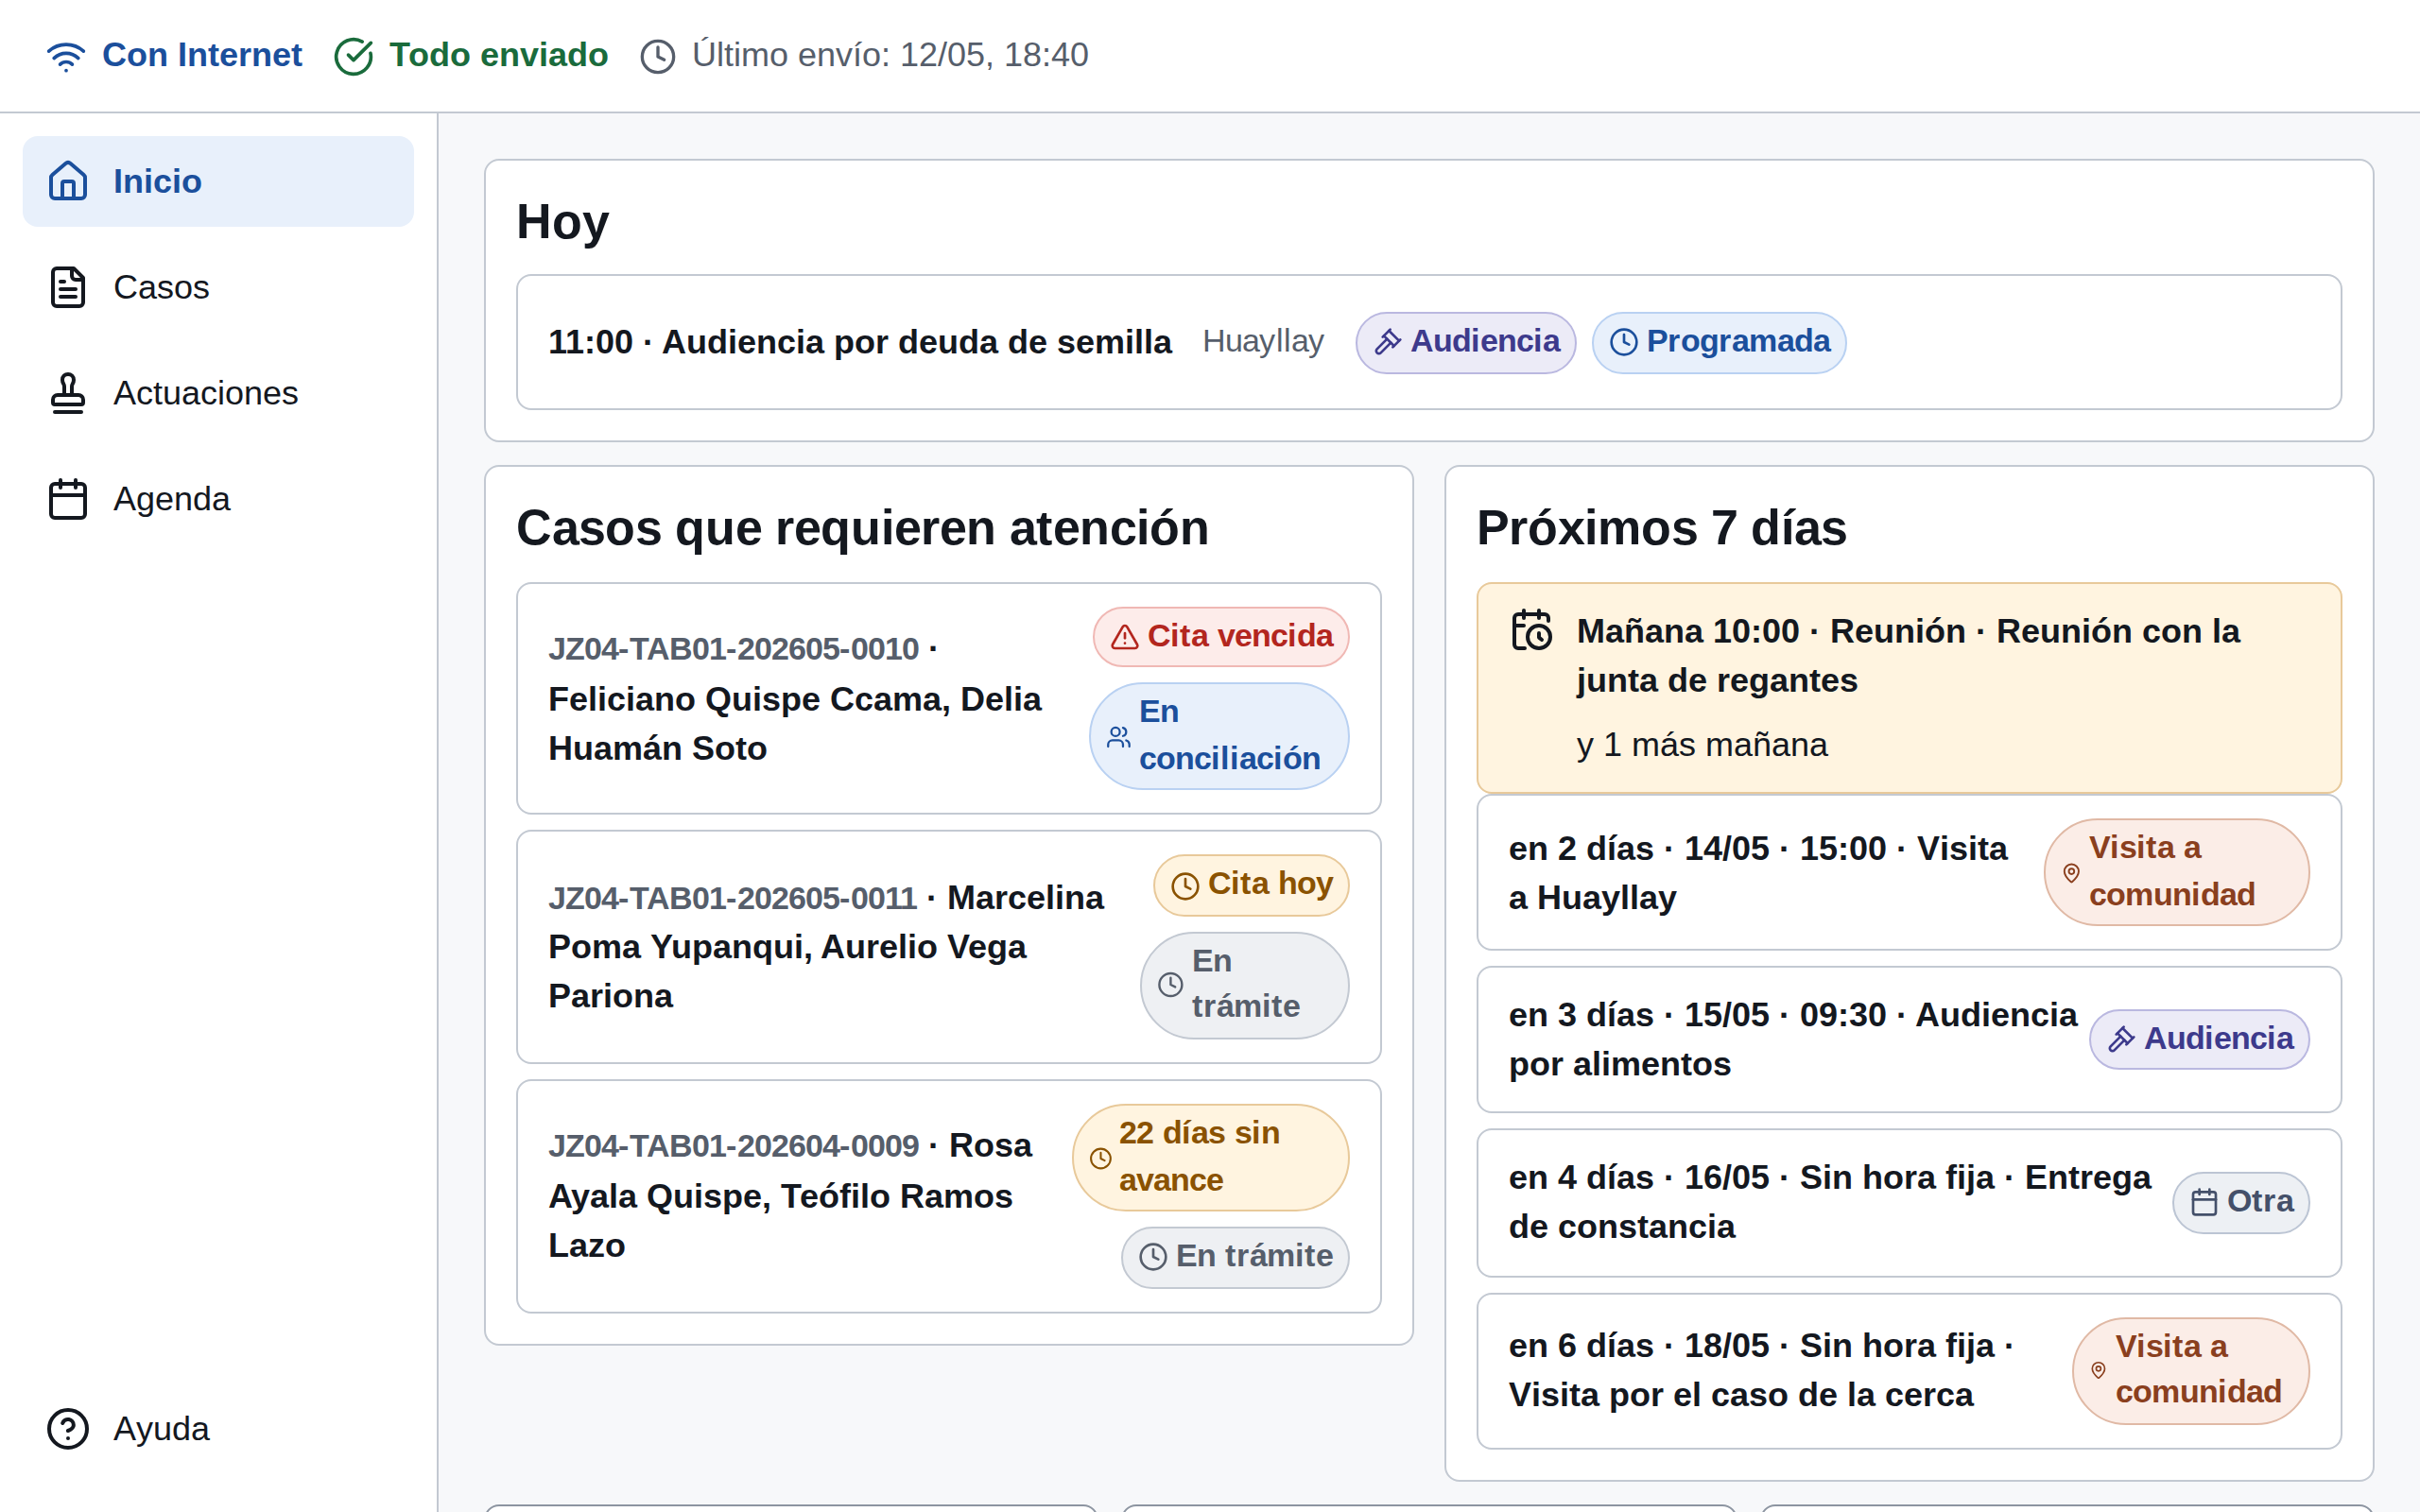
\includegraphics[width=0.82\linewidth]{capturas/F1-01_inicio.png}
\caption{P-01 · 1. Inicio con Internet y todo enviado. Punto de partida: barra en Con Internet y Todo enviado}
\end{figure}
\begin{figure}[H]\centering
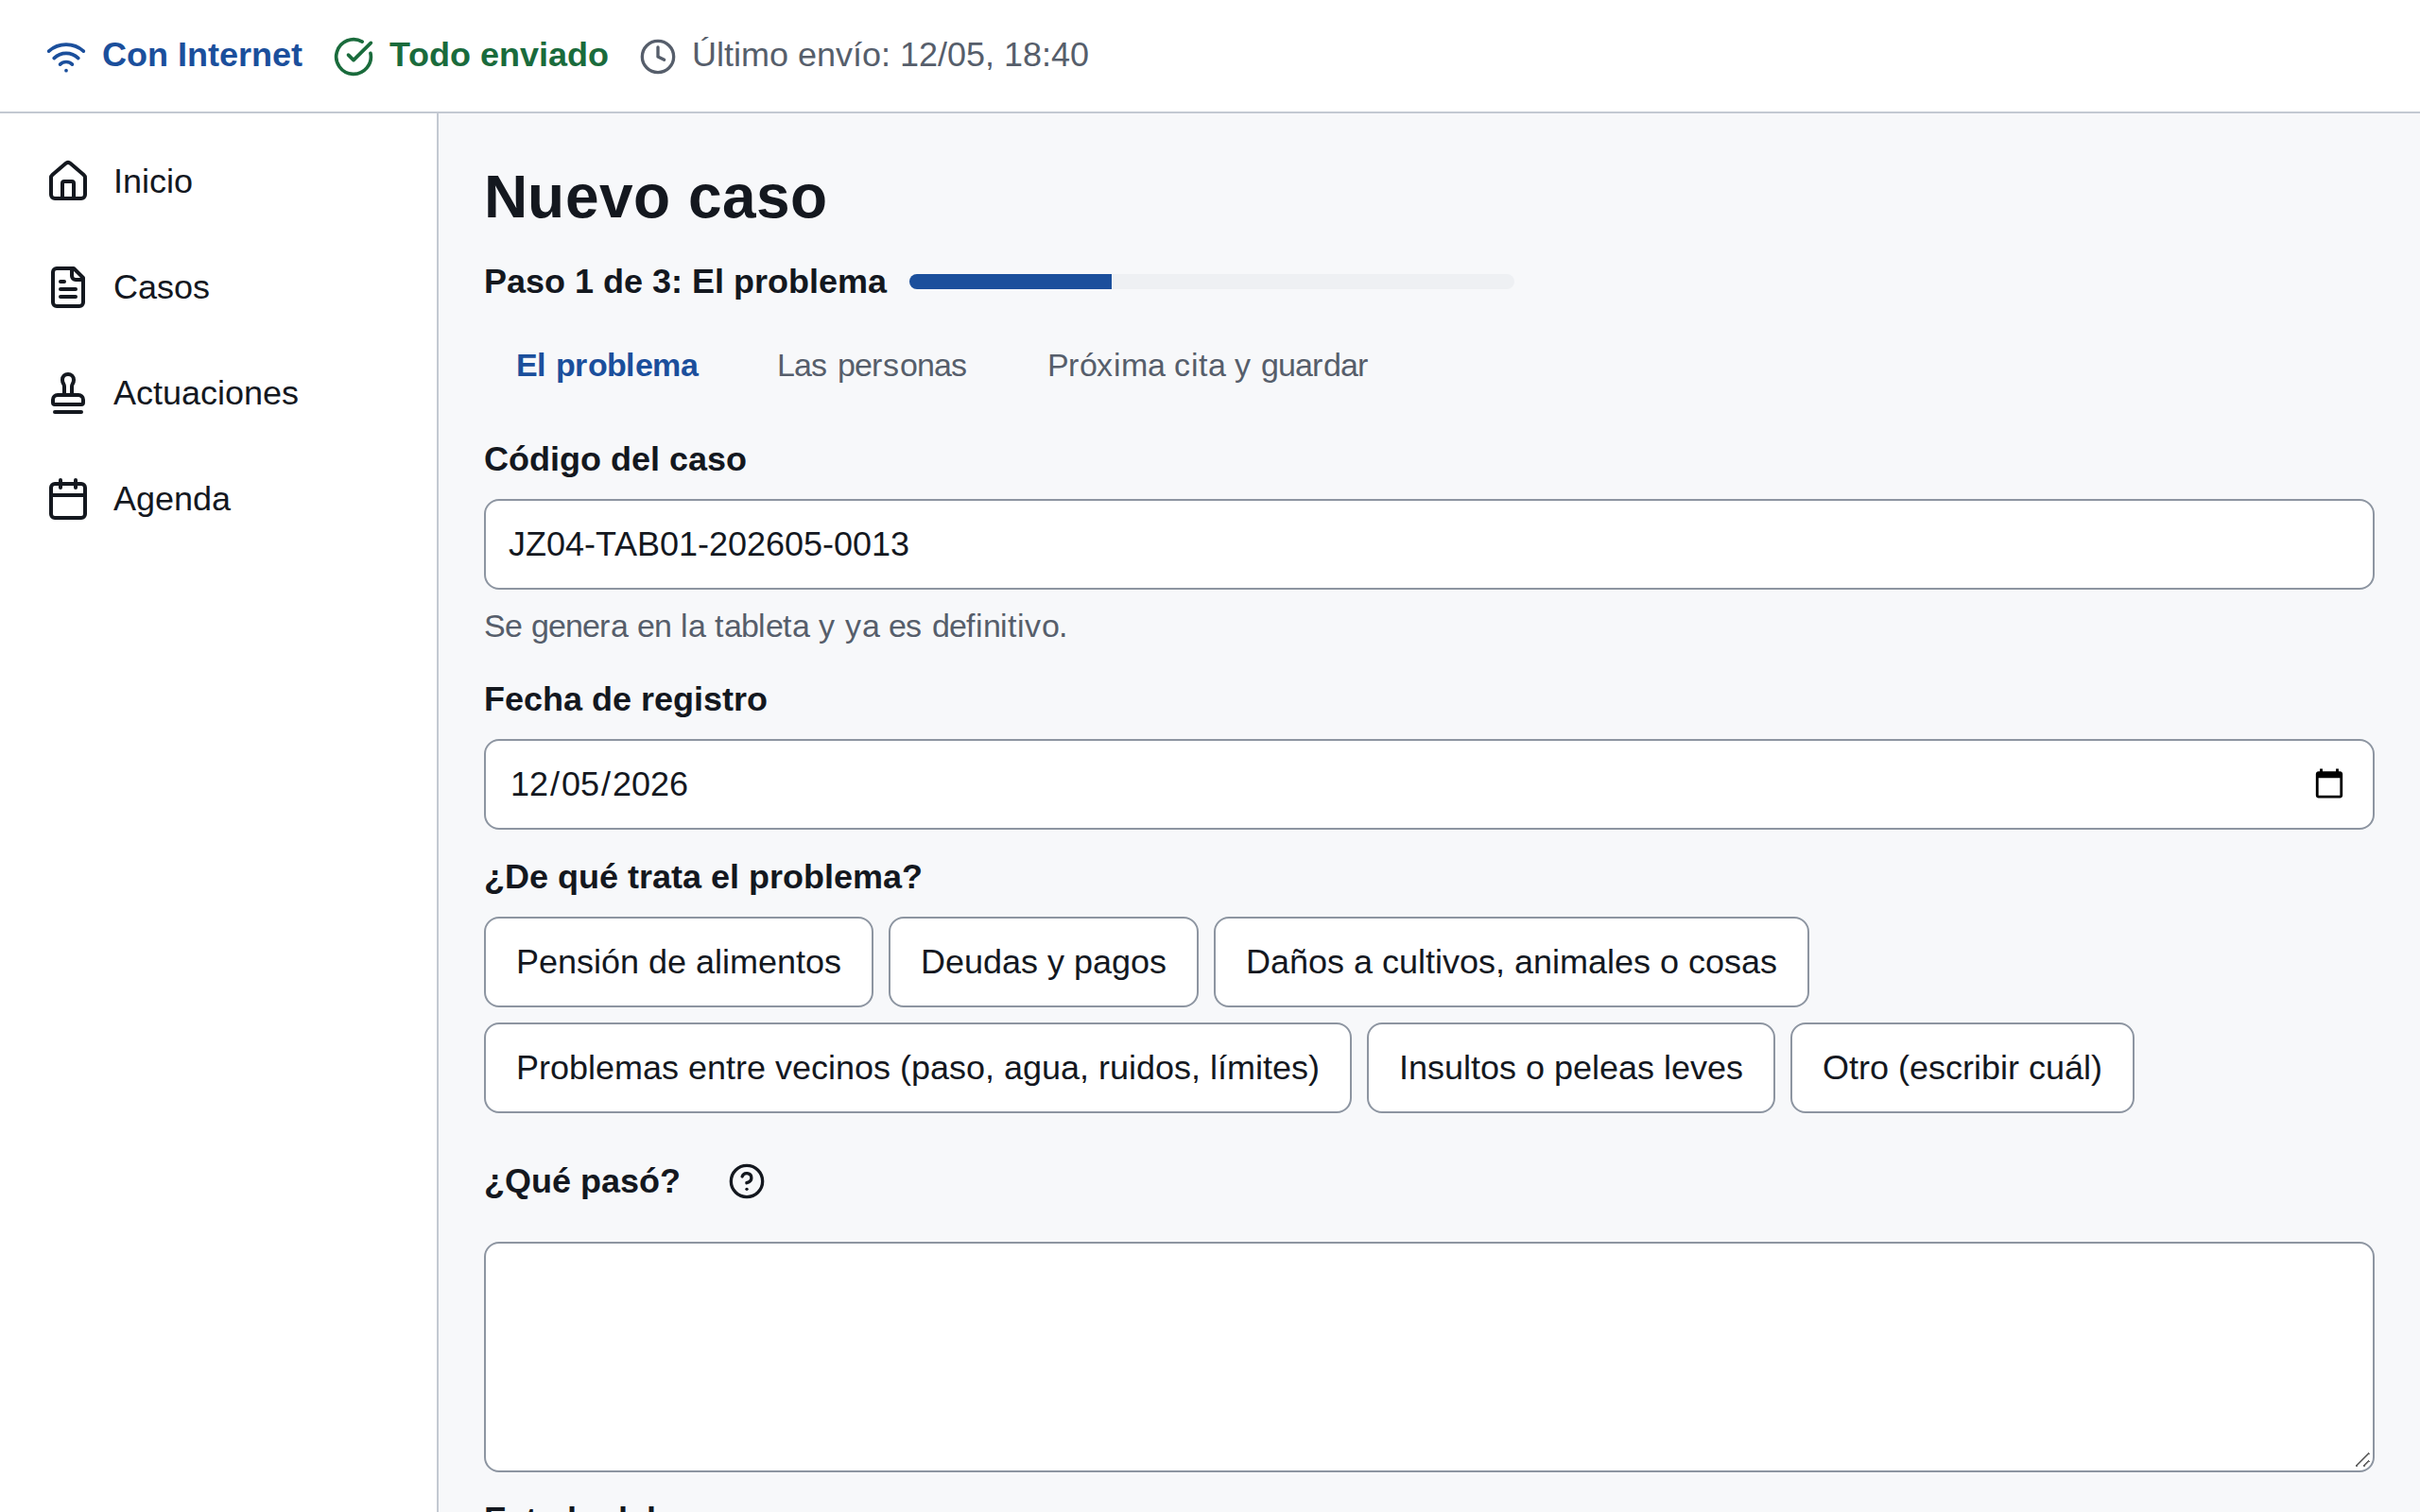
\includegraphics[width=0.82\linewidth]{capturas/F1-02_caso-paso1.png}
\caption{P-03 · 2. Paso 1, el problema. Código generado en la tableta y catálogo de tipos de problema en botones grandes}
\end{figure}
\begin{figure}[H]\centering
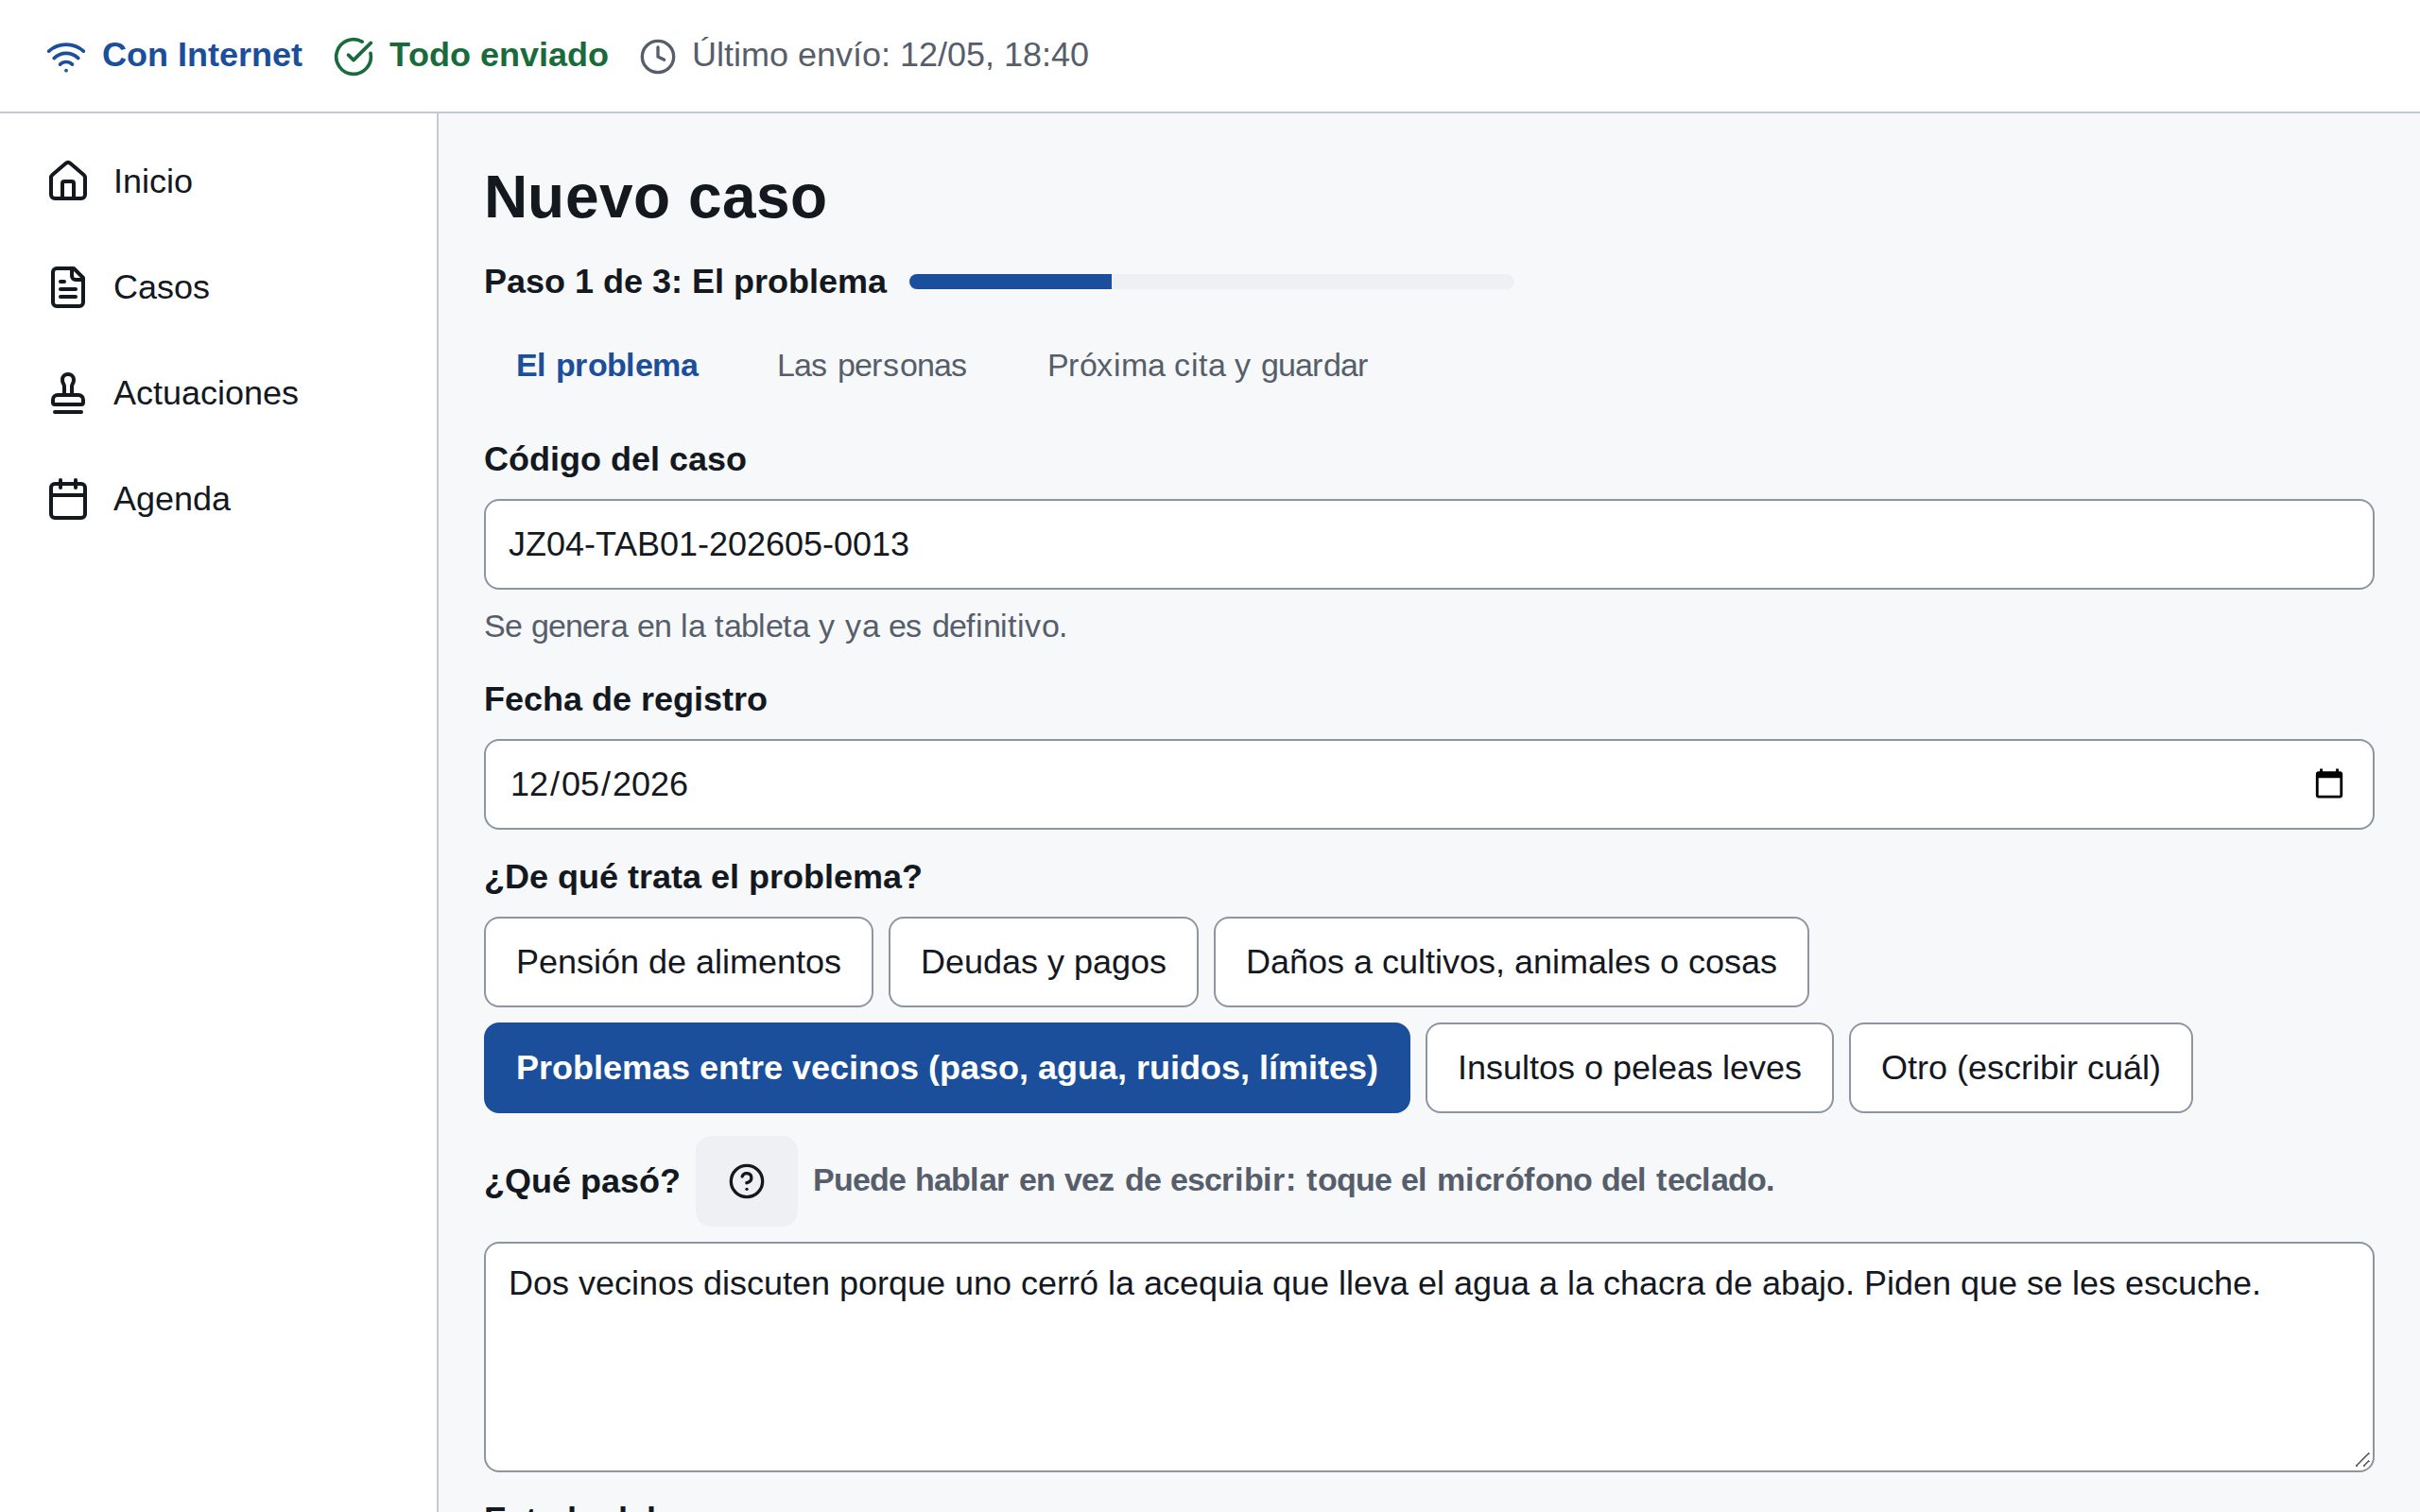
\includegraphics[width=0.82\linewidth]{capturas/F1-03_caso-paso1-lleno.png}
\caption{P-03 · 2. Paso 1 completo. Descripción con la ayuda para dictar desde el teclado, sin micrófono propio}
\end{figure}
\begin{figure}[H]\centering
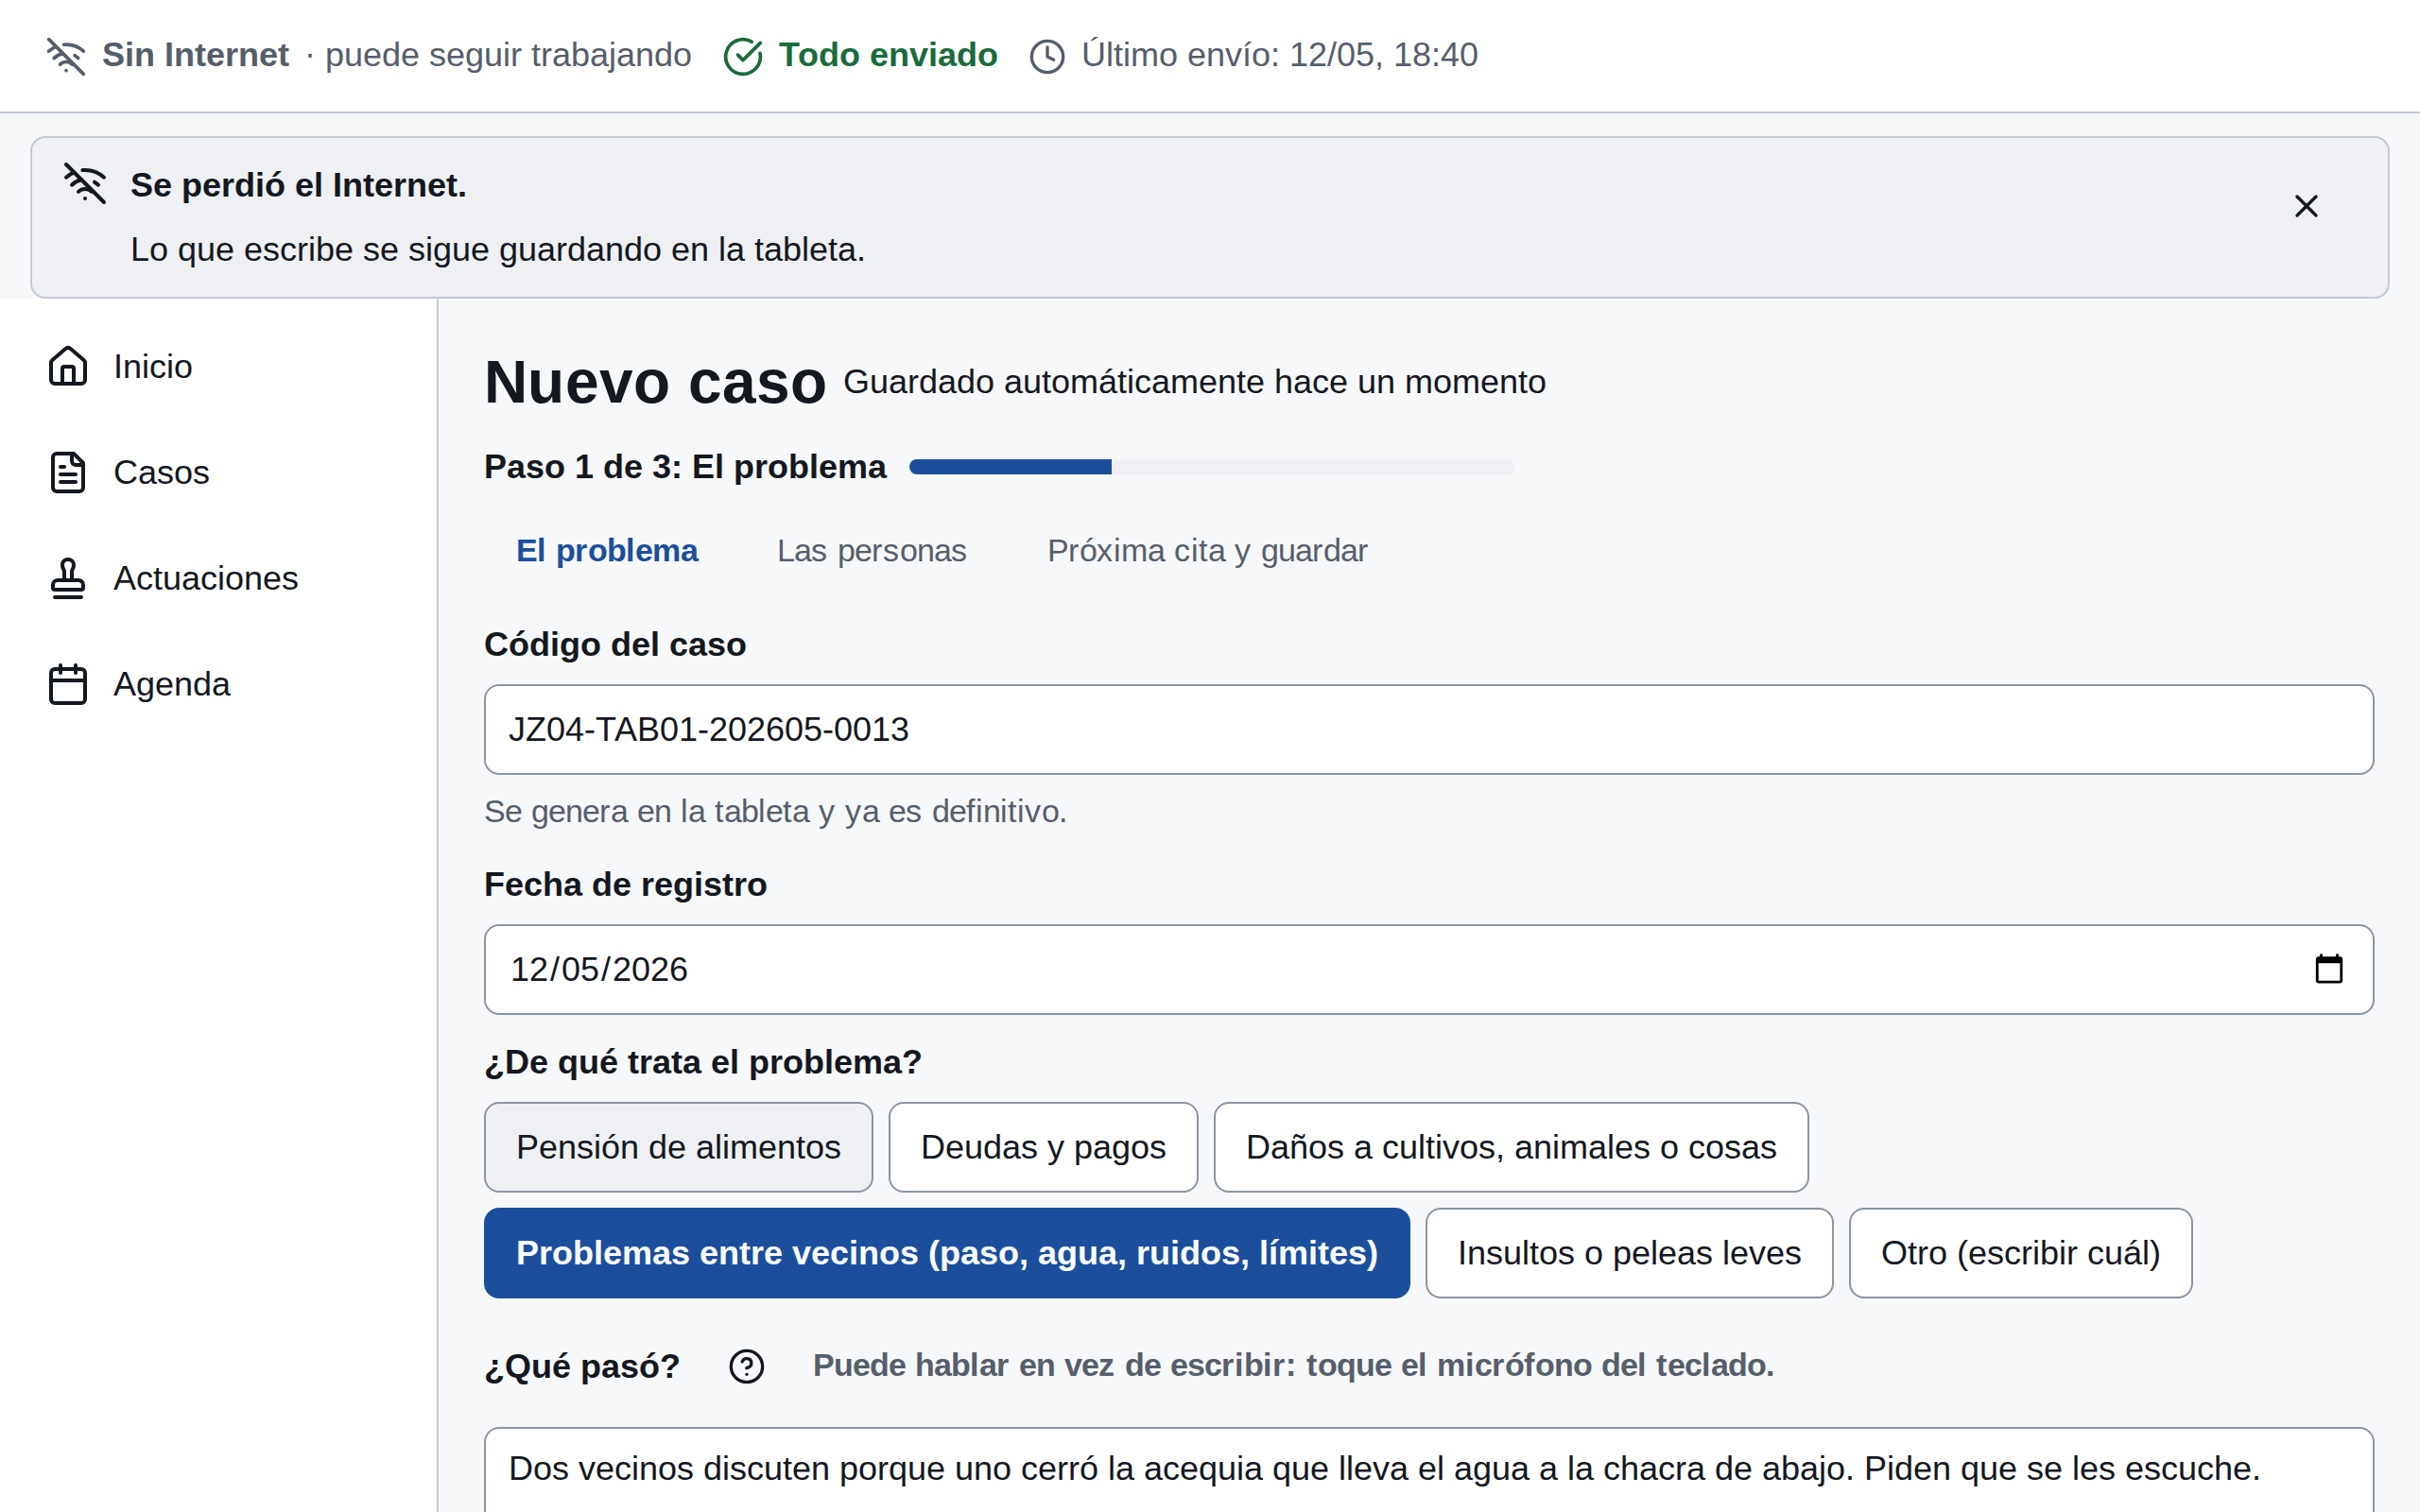
\includegraphics[width=0.82\linewidth]{capturas/F1-04_corte-internet.png}
\caption{P-03 · 3. Se corta el Internet a mitad del formulario. Aviso de corte sin alarma y barra en Sin Internet, en gris; el trabajo continúa}
\end{figure}
\begin{figure}[H]\centering
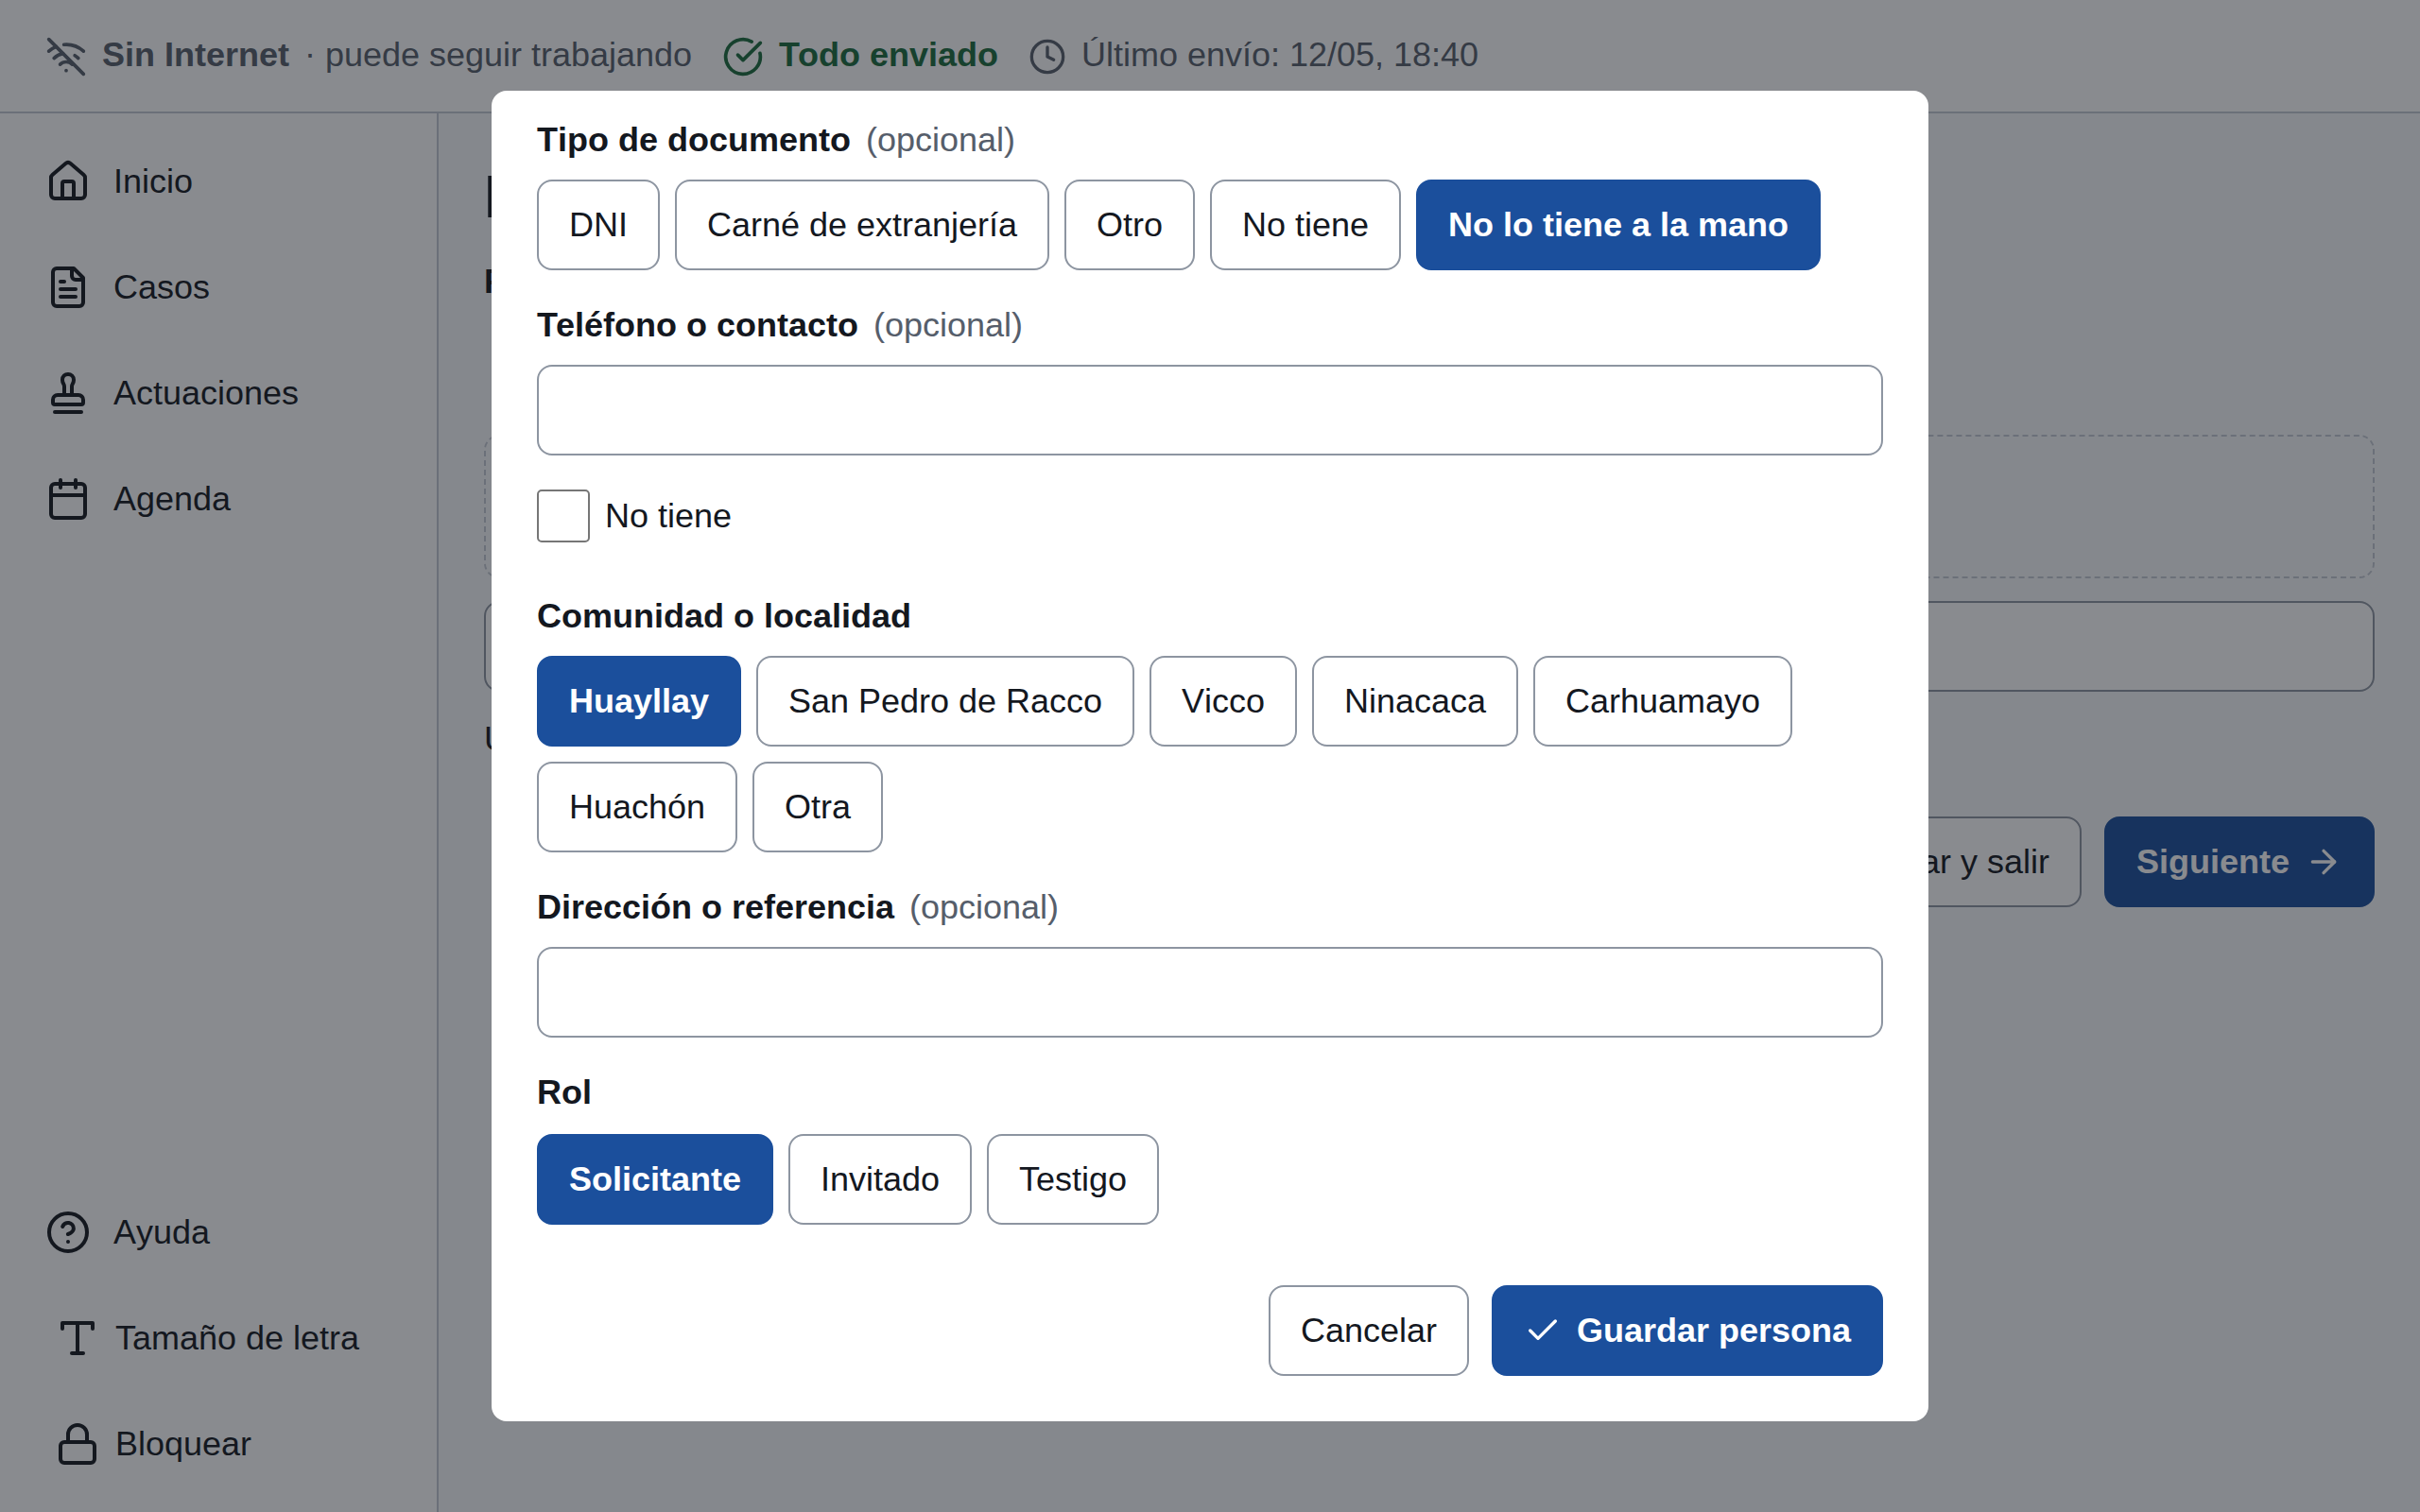
\includegraphics[width=0.82\linewidth]{capturas/F1-05_persona-1.png}
\caption{P-03 · 4. Primera parte, sin documento a la mano. Opción No lo tiene a la mano en vez de obligar un DNI inventado}
\end{figure}
\begin{figure}[H]\centering
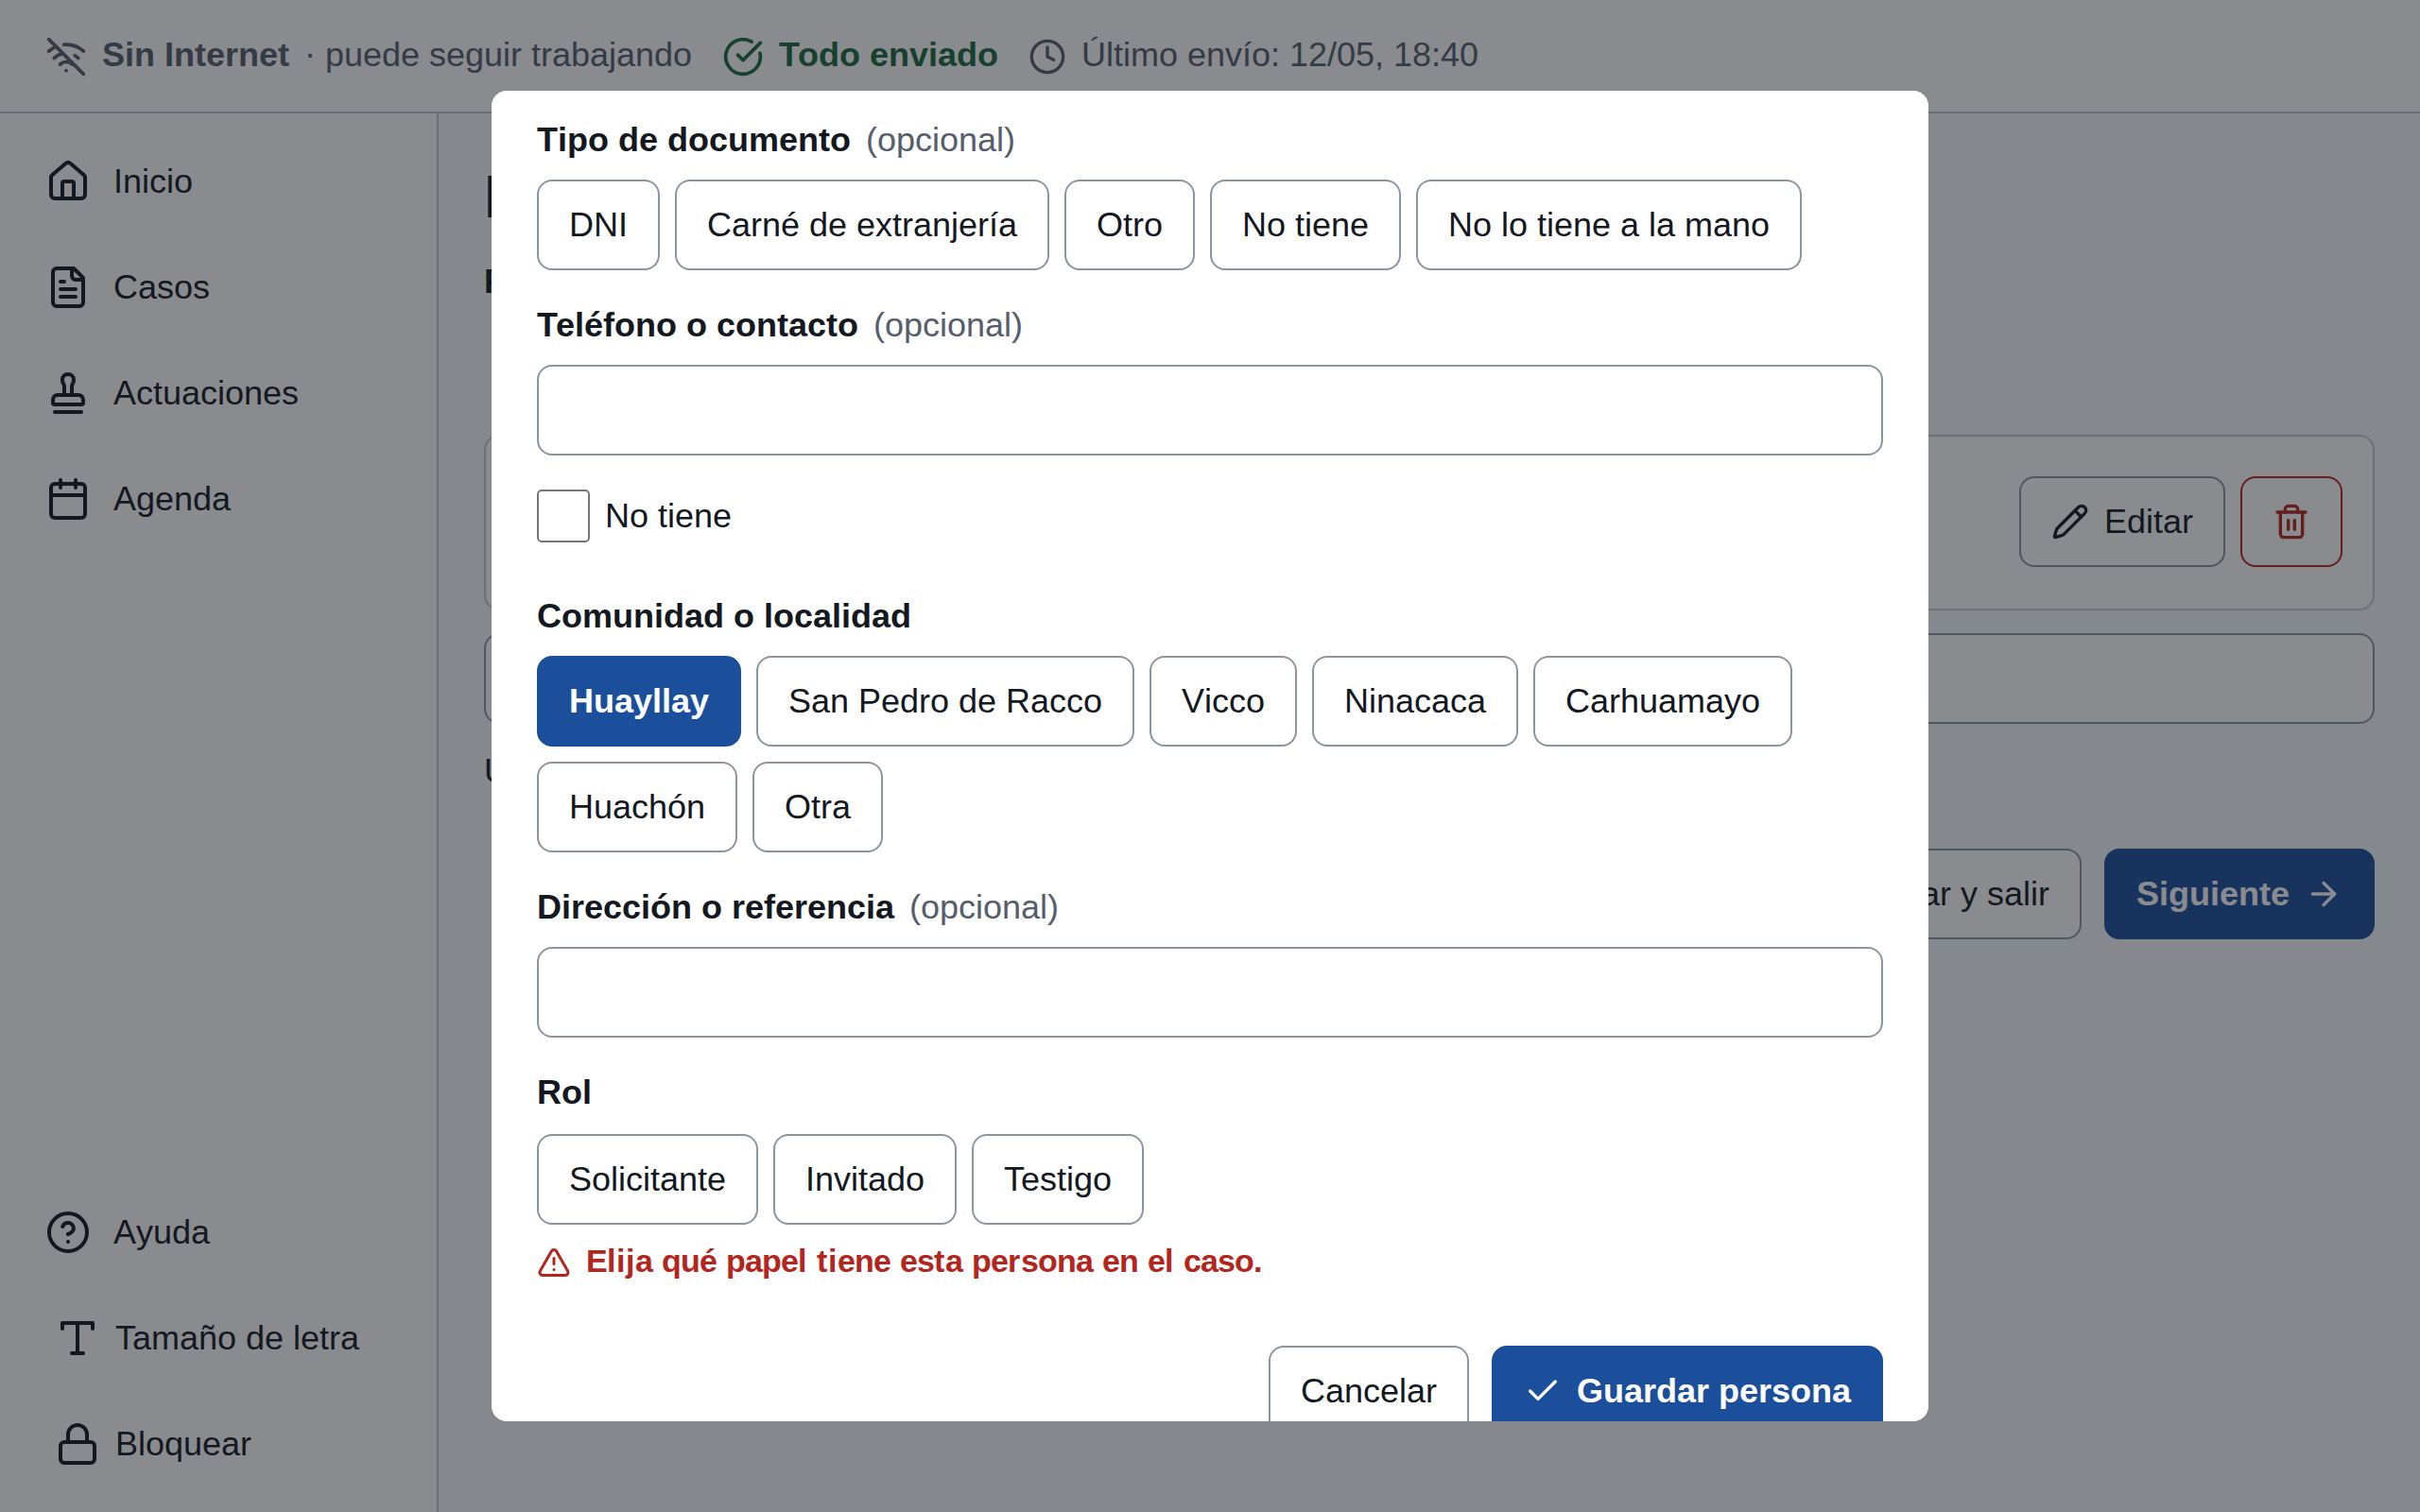
\includegraphics[width=0.82\linewidth]{capturas/F1-06_error-rol.png}
\caption{P-03 · 6. Error de validación en lenguaje simple. Mensaje que dice qué falta y cómo resolverlo, sin jerga}
\end{figure}
\begin{figure}[H]\centering
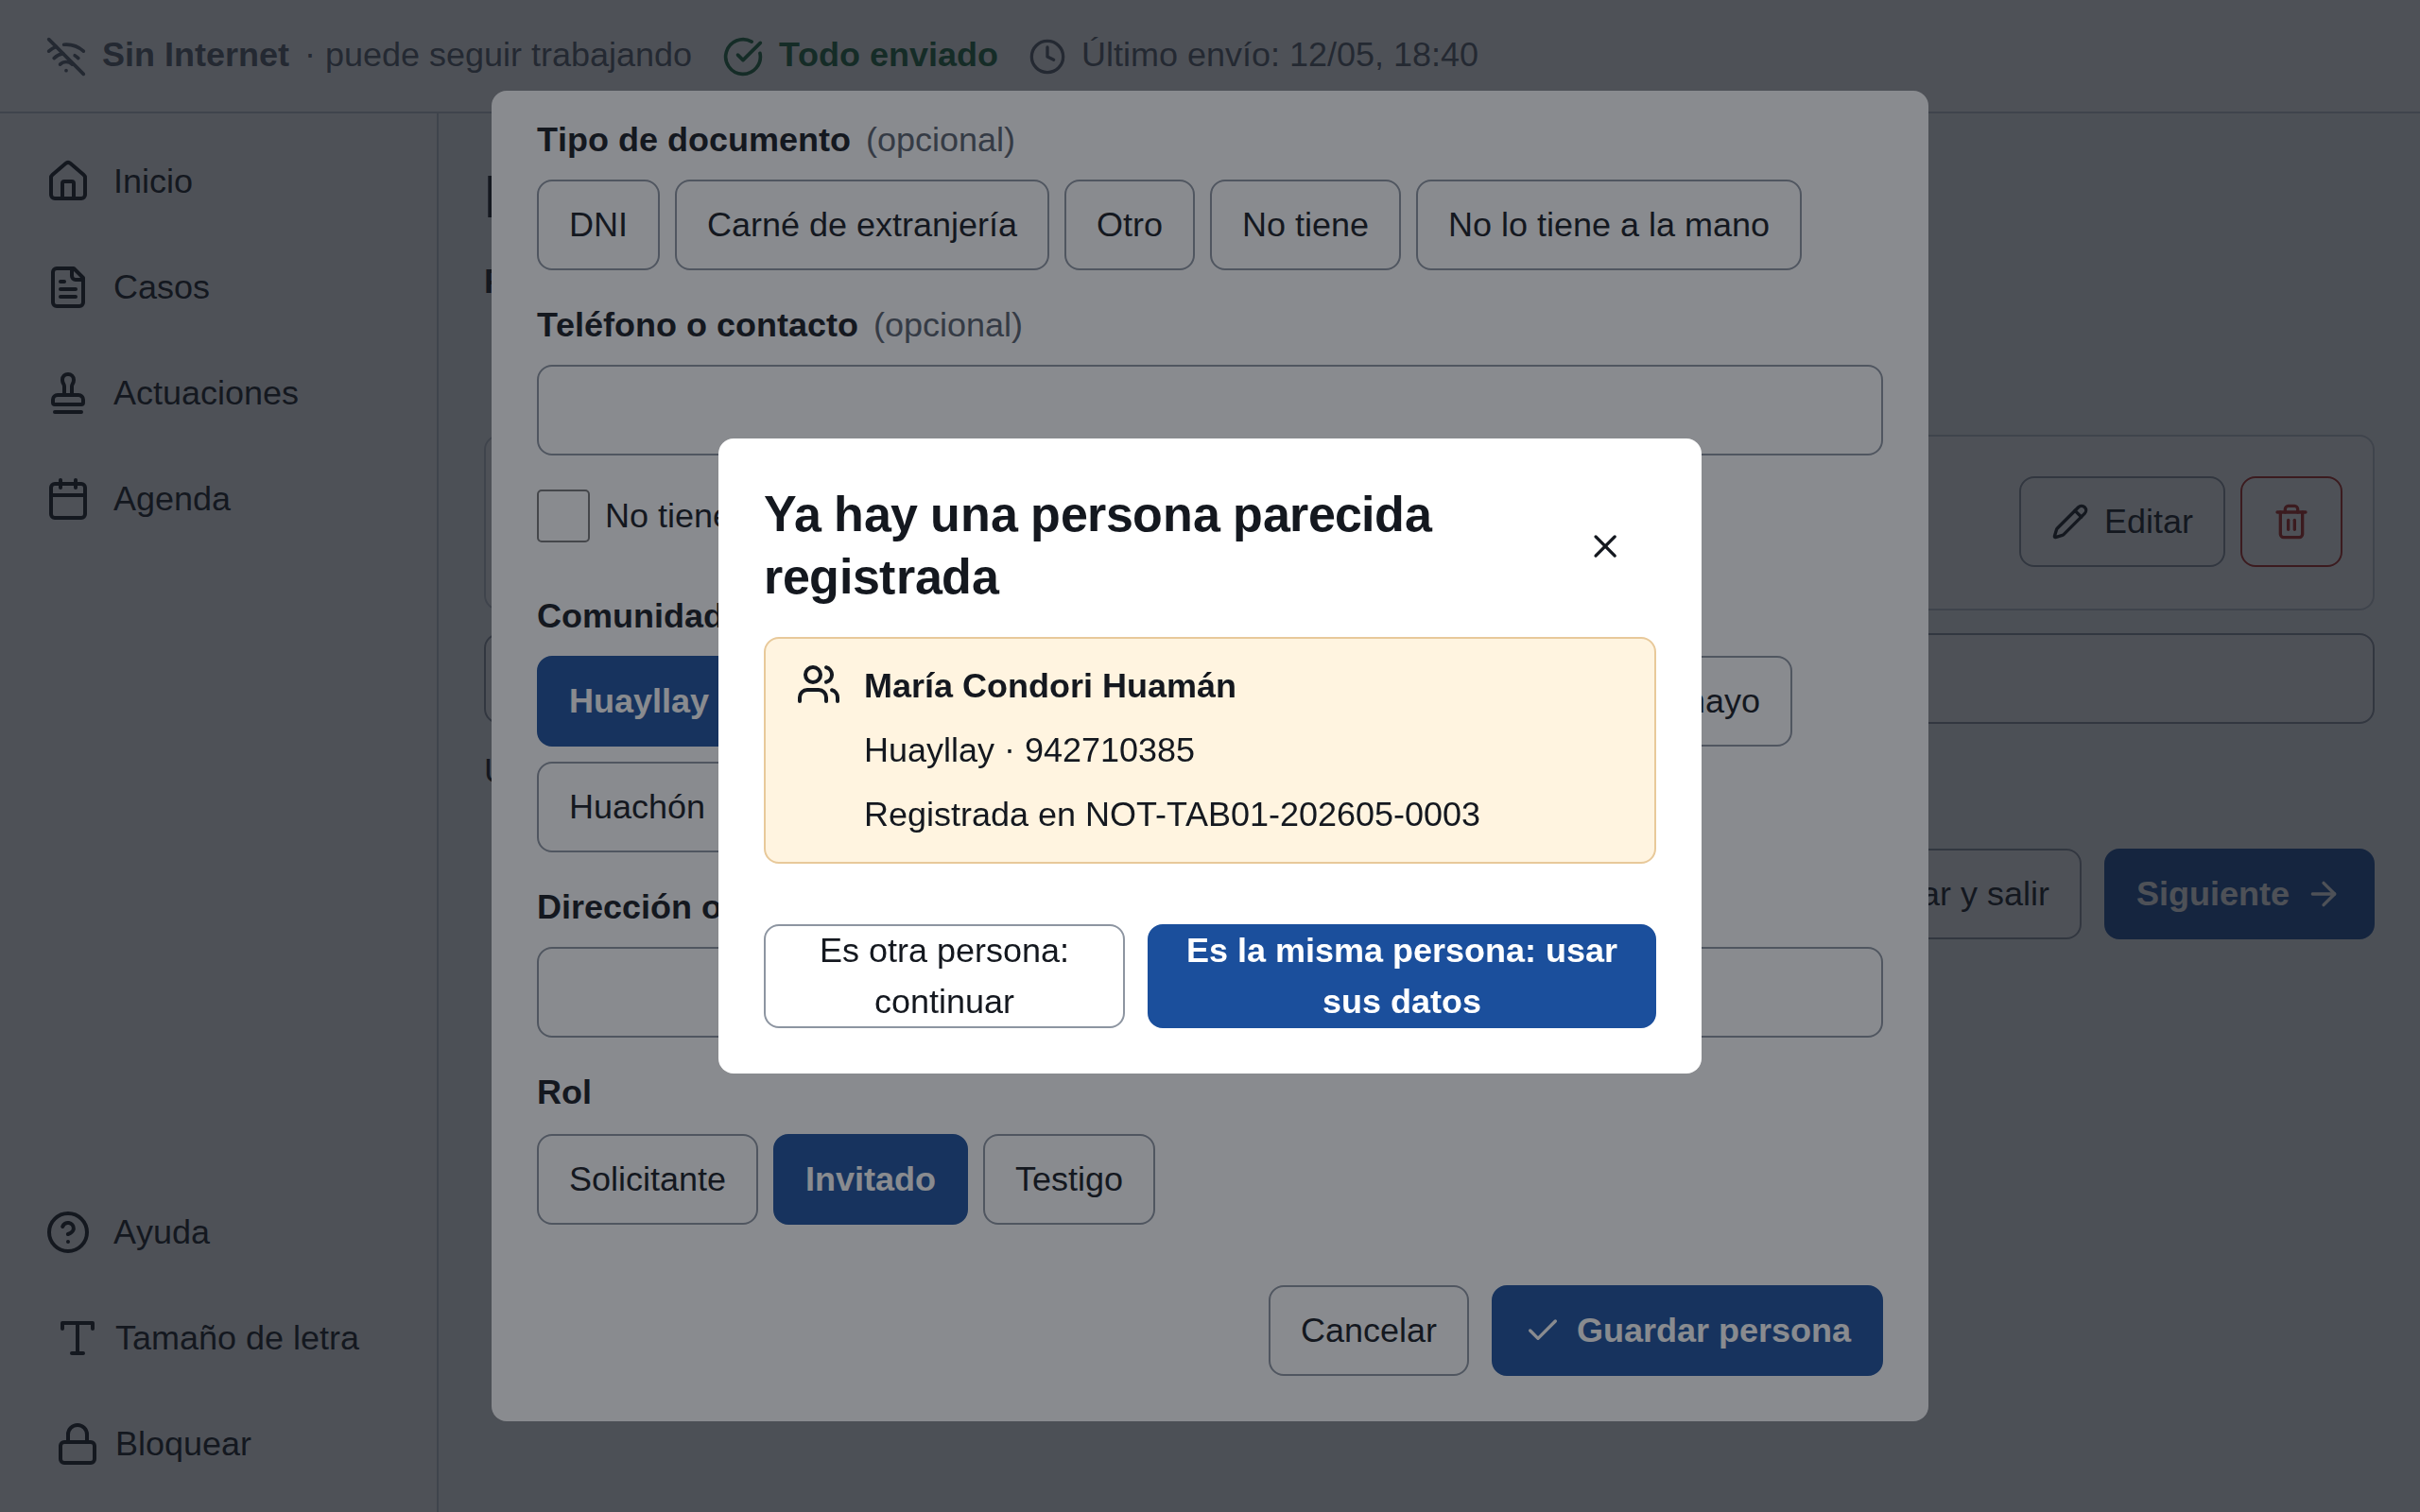
\includegraphics[width=0.82\linewidth]{capturas/F1-07_duplicado.png}
\caption{P-03 · 5. Advertencia de persona duplicada. Advierte sin bloquear y deja elegir entre usar sus datos o continuar}
\end{figure}
\begin{figure}[H]\centering
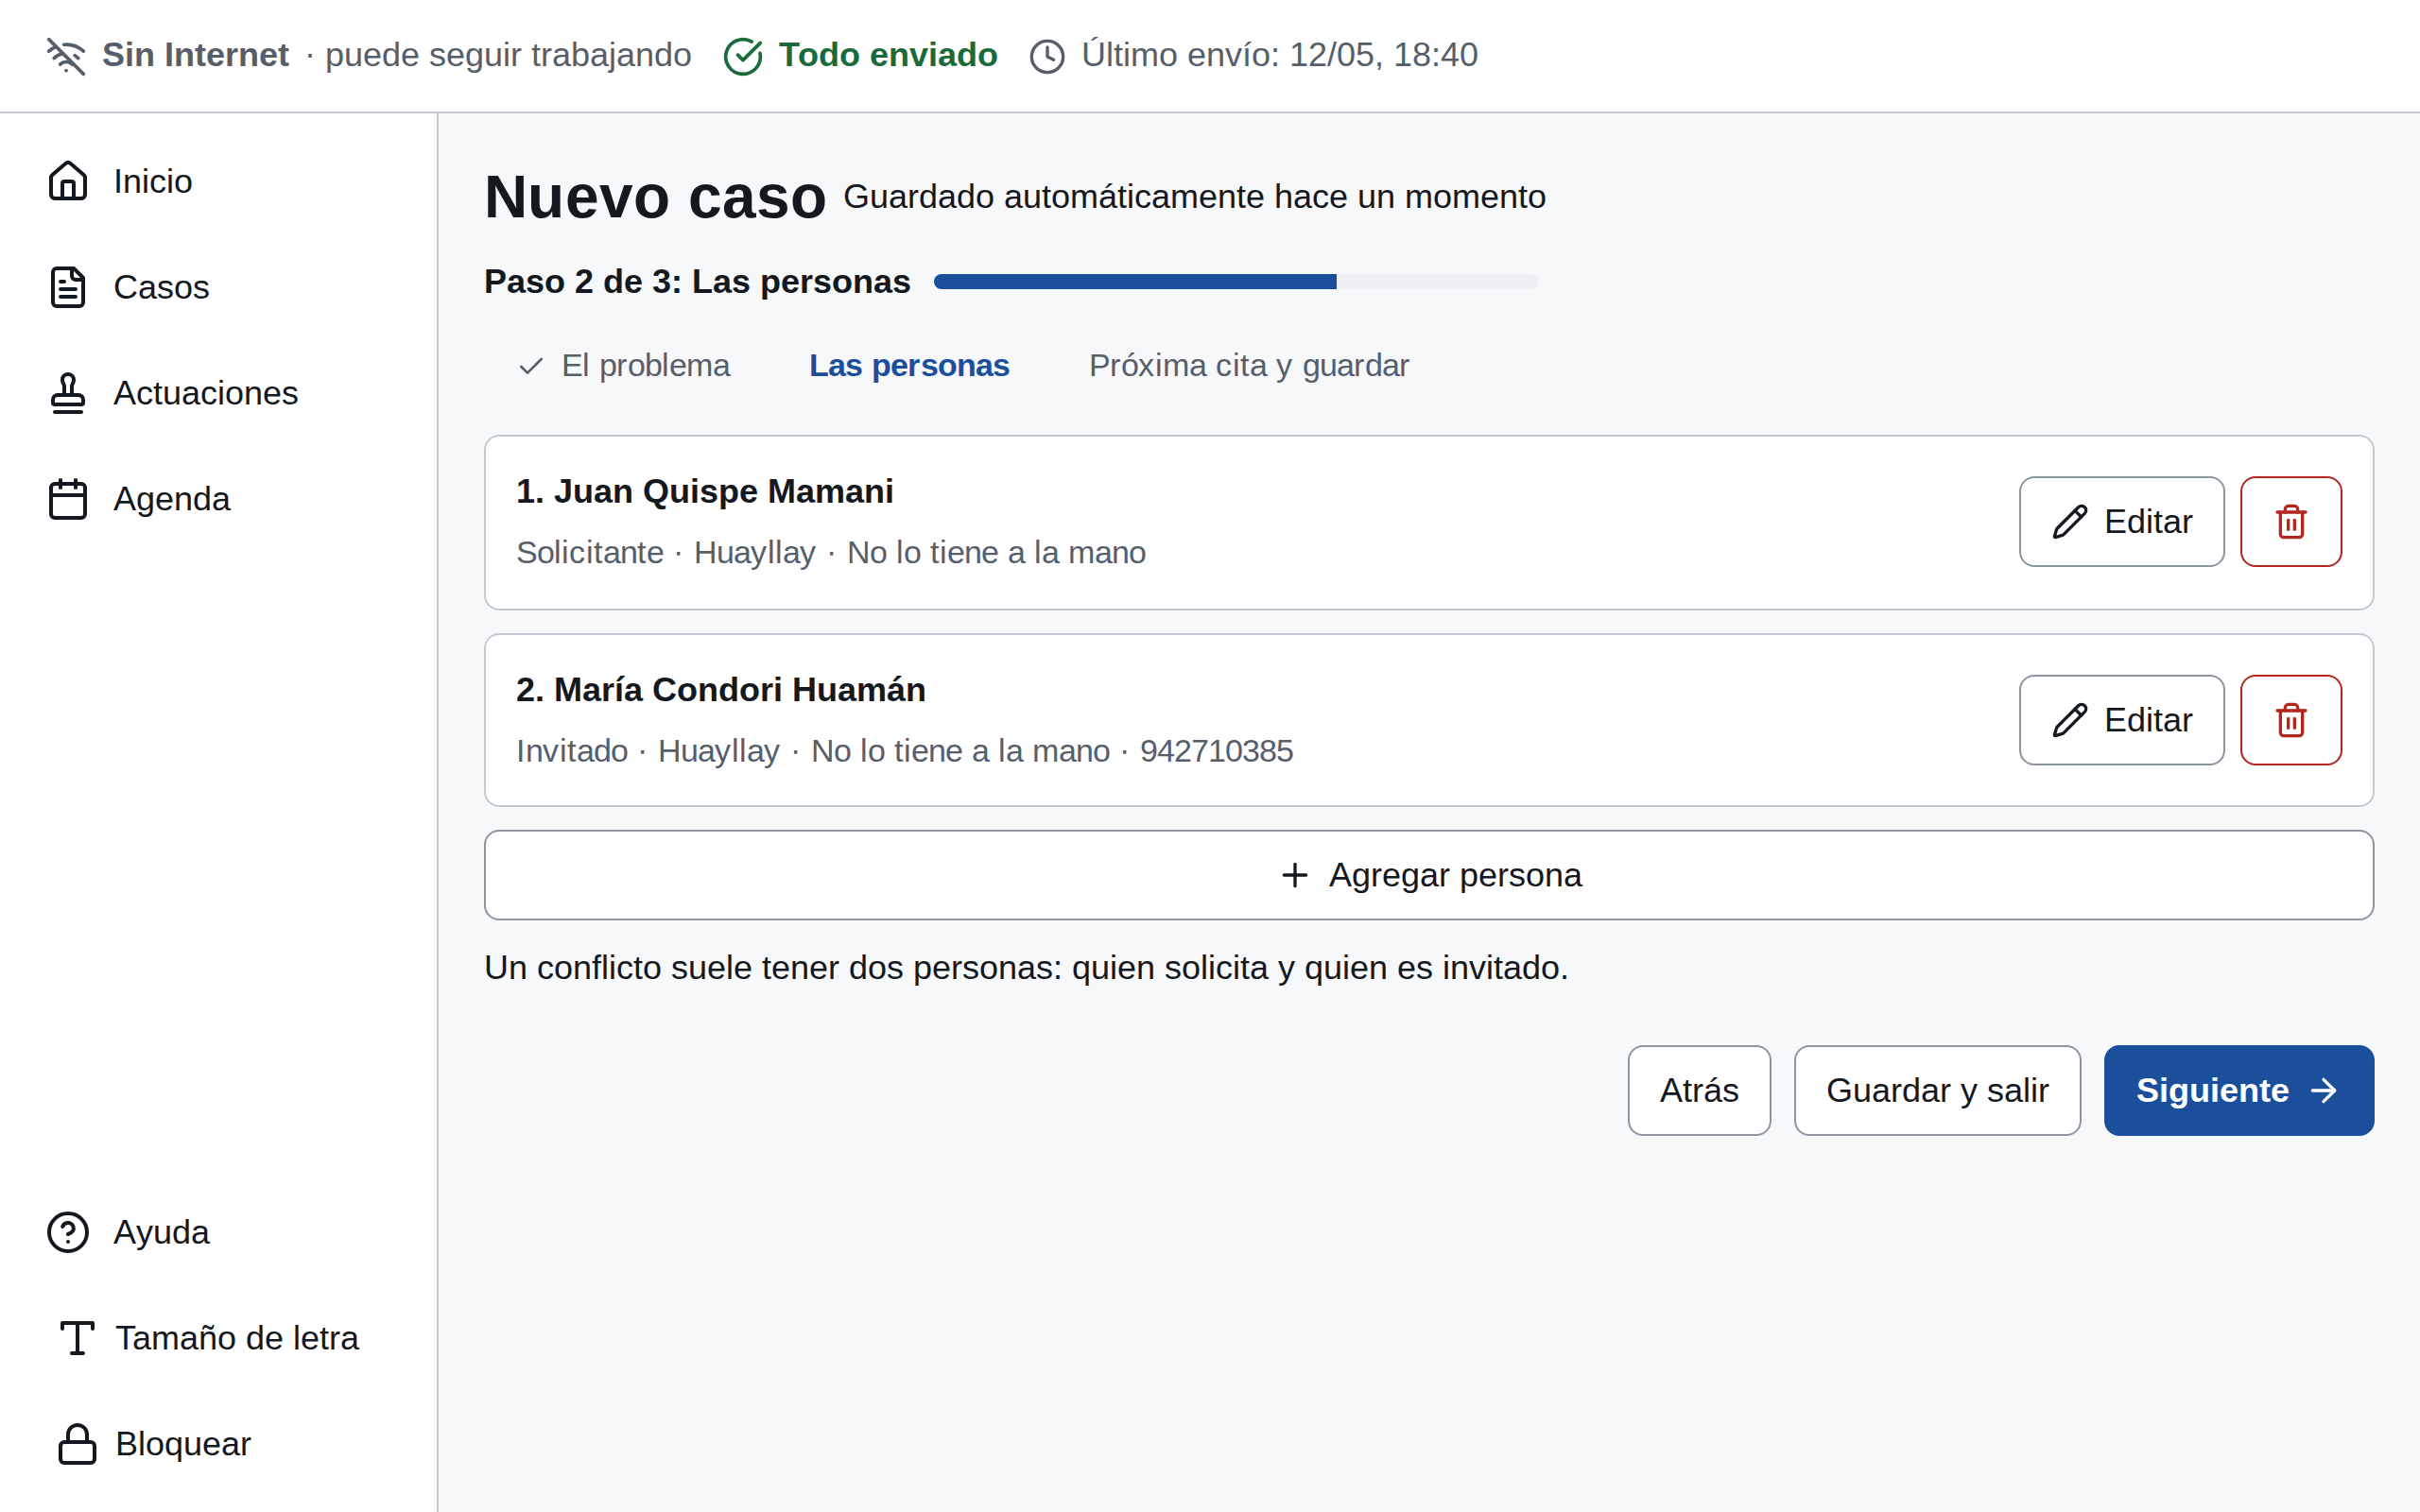
\includegraphics[width=0.82\linewidth]{capturas/F1-08_personas.png}
\caption{P-03 · 5. Las dos partes con su rol. Las partes quedan con rol y comunidad visibles}
\end{figure}
\begin{figure}[H]\centering
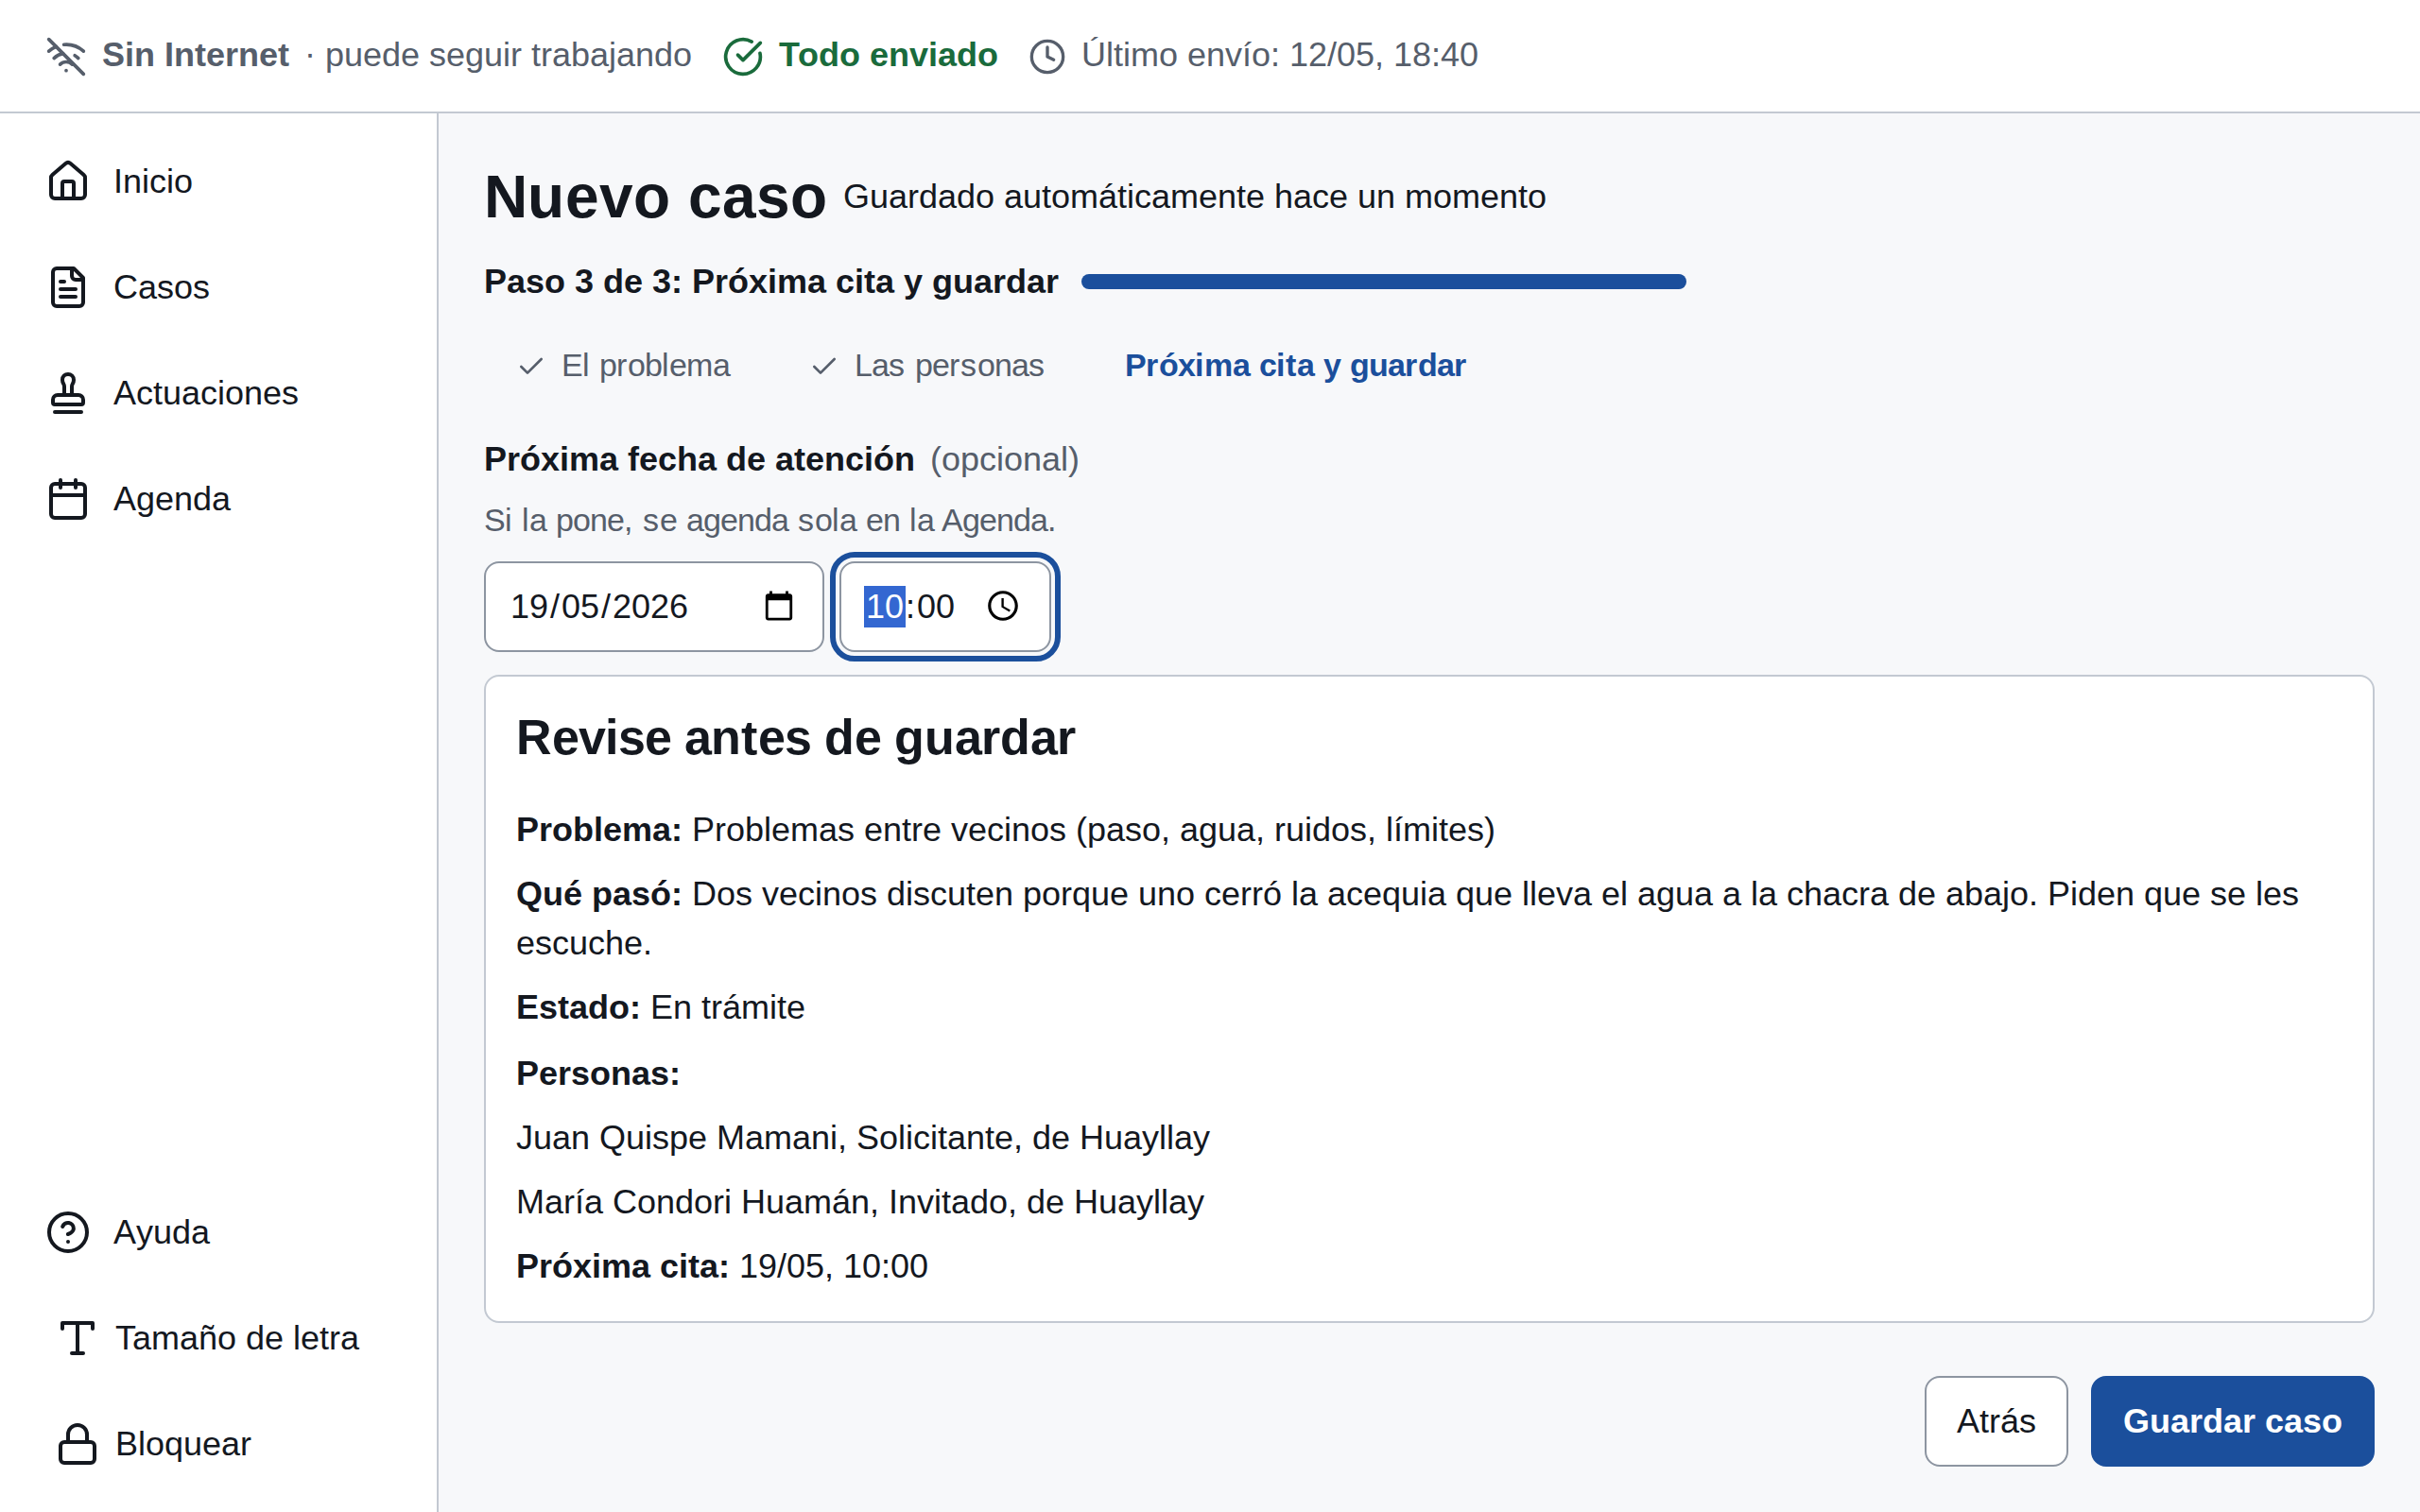
\includegraphics[width=0.82\linewidth]{capturas/F1-09_resumen.png}
\caption{P-03 · 7. Resumen antes de guardar. Resumen legible para leerlo en voz alta a las partes antes de guardar}
\end{figure}
\begin{figure}[H]\centering
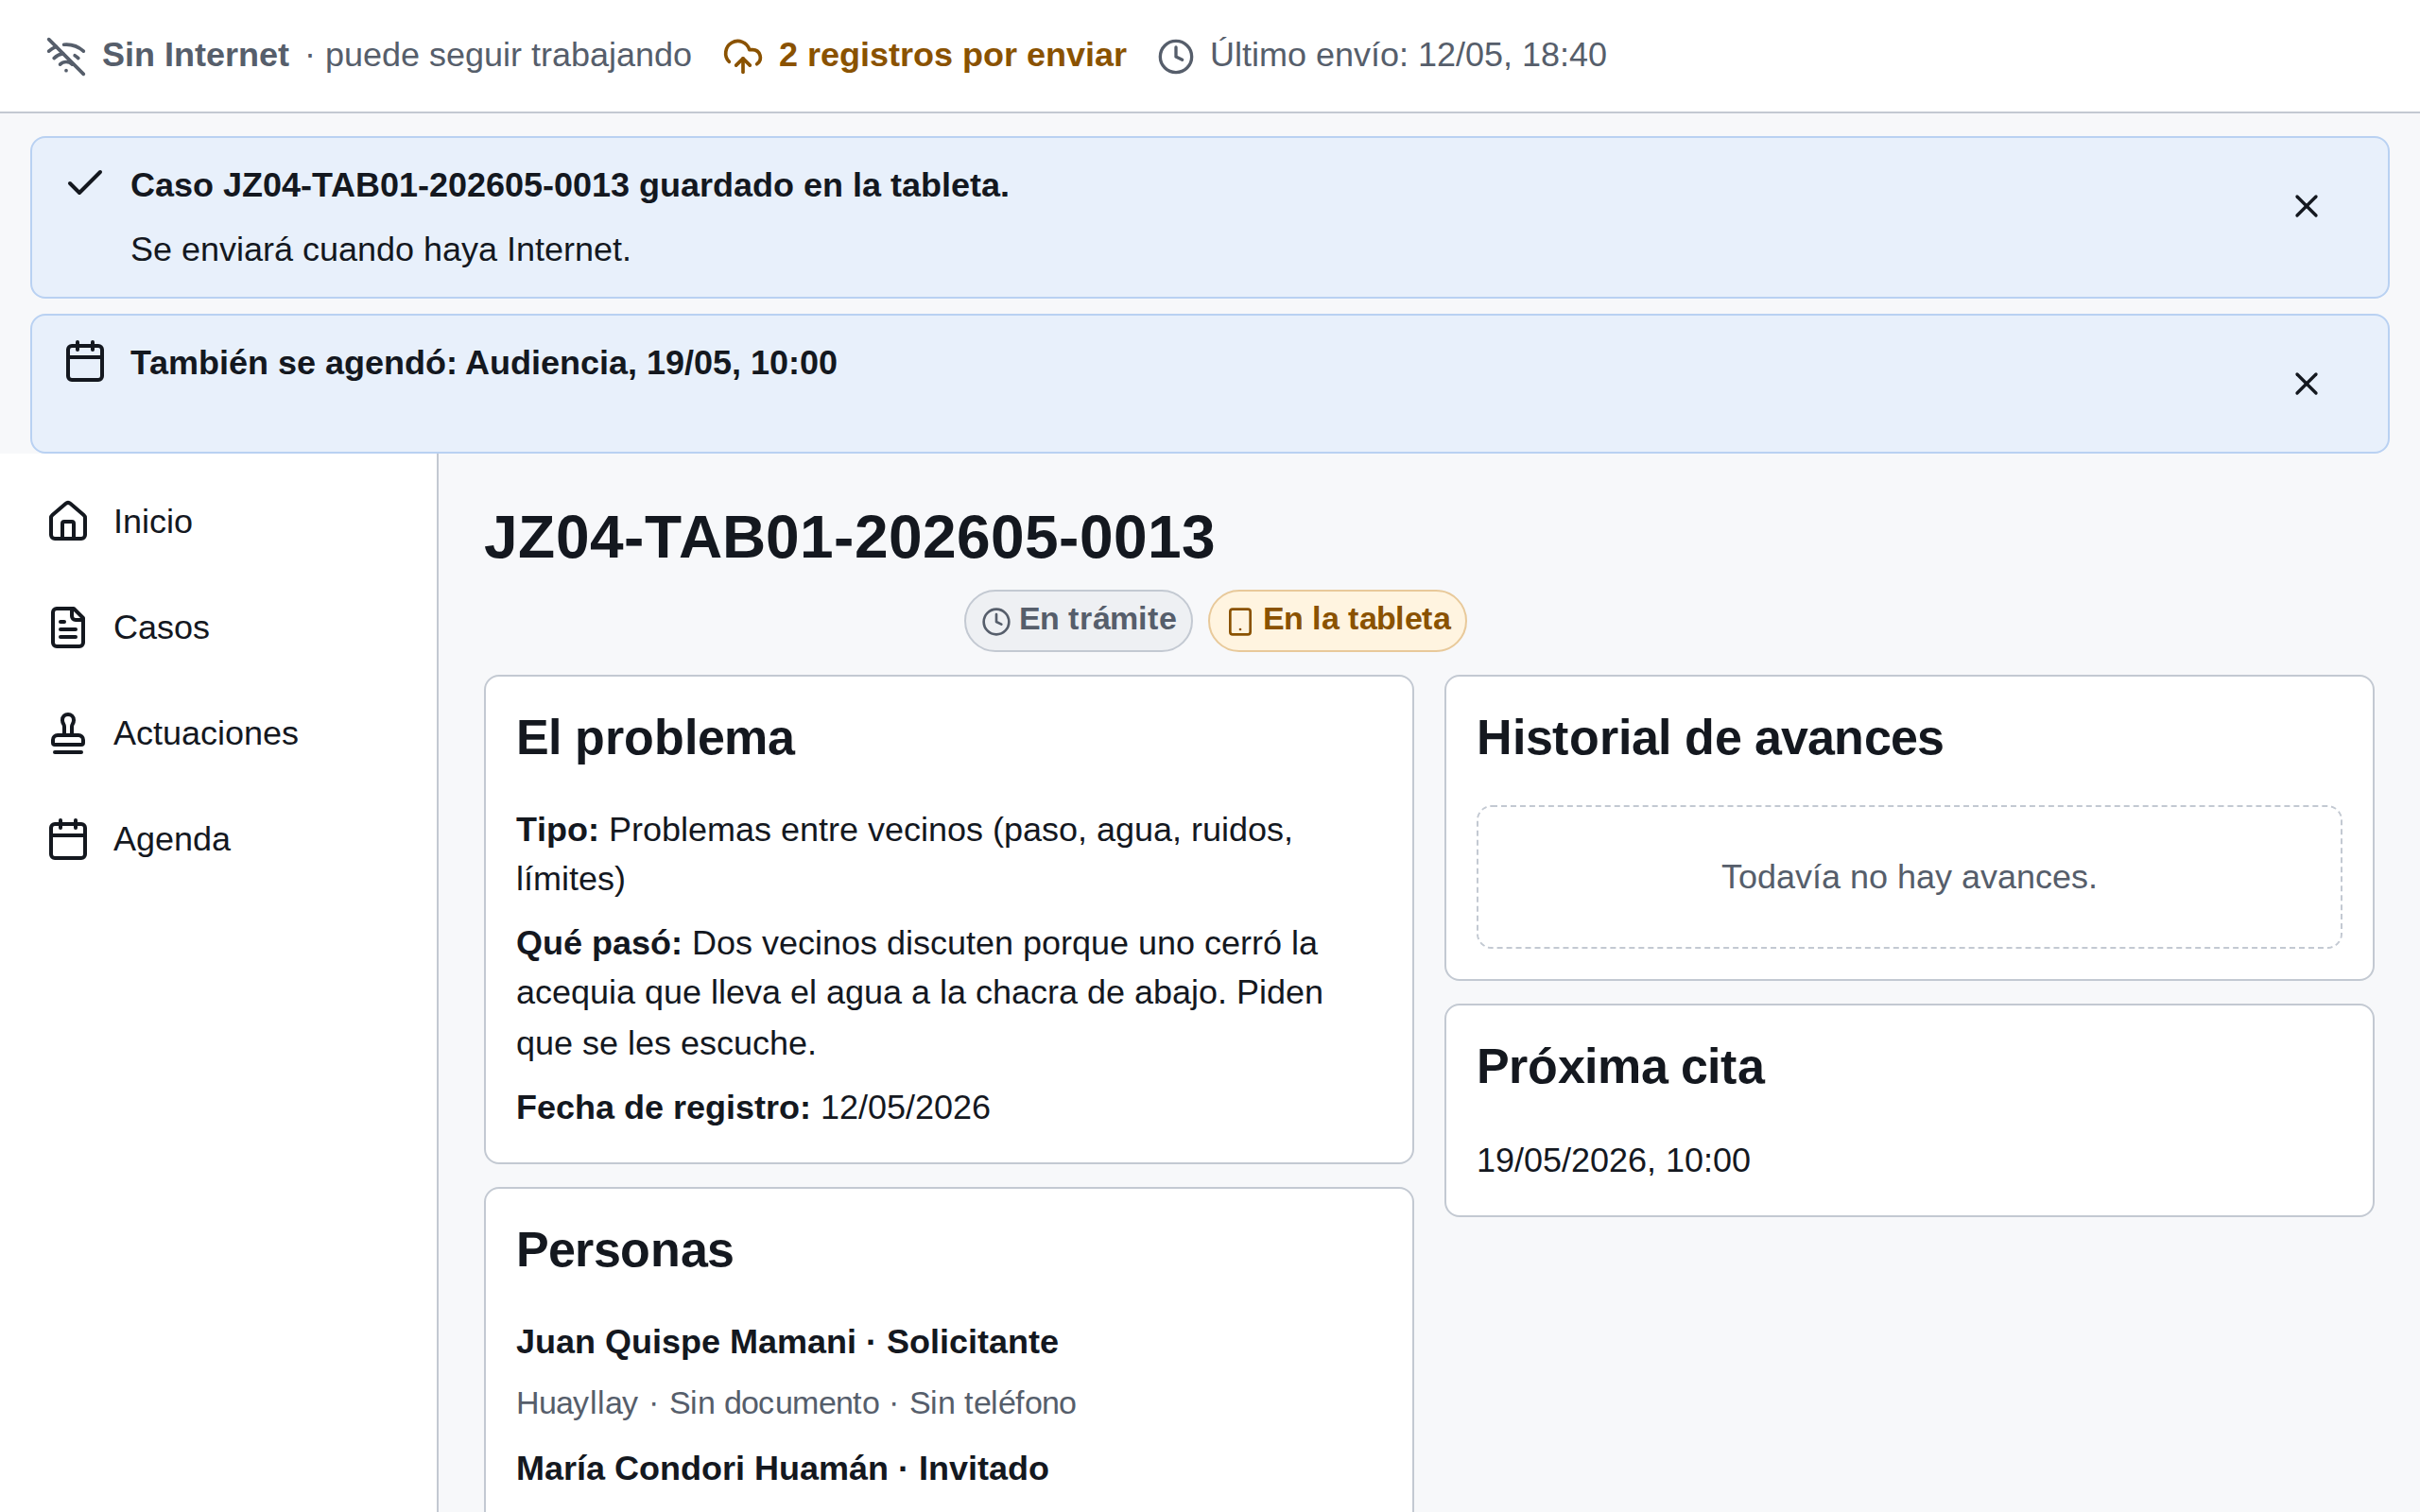
\includegraphics[width=0.82\linewidth]{capturas/F1-10_confirmacion-guardado.png}
\caption{P-04 · 8. Confirmación de guardado. La confirmación dice dónde quedó el caso y que también se agendó la cita}
\end{figure}
\begin{figure}[H]\centering
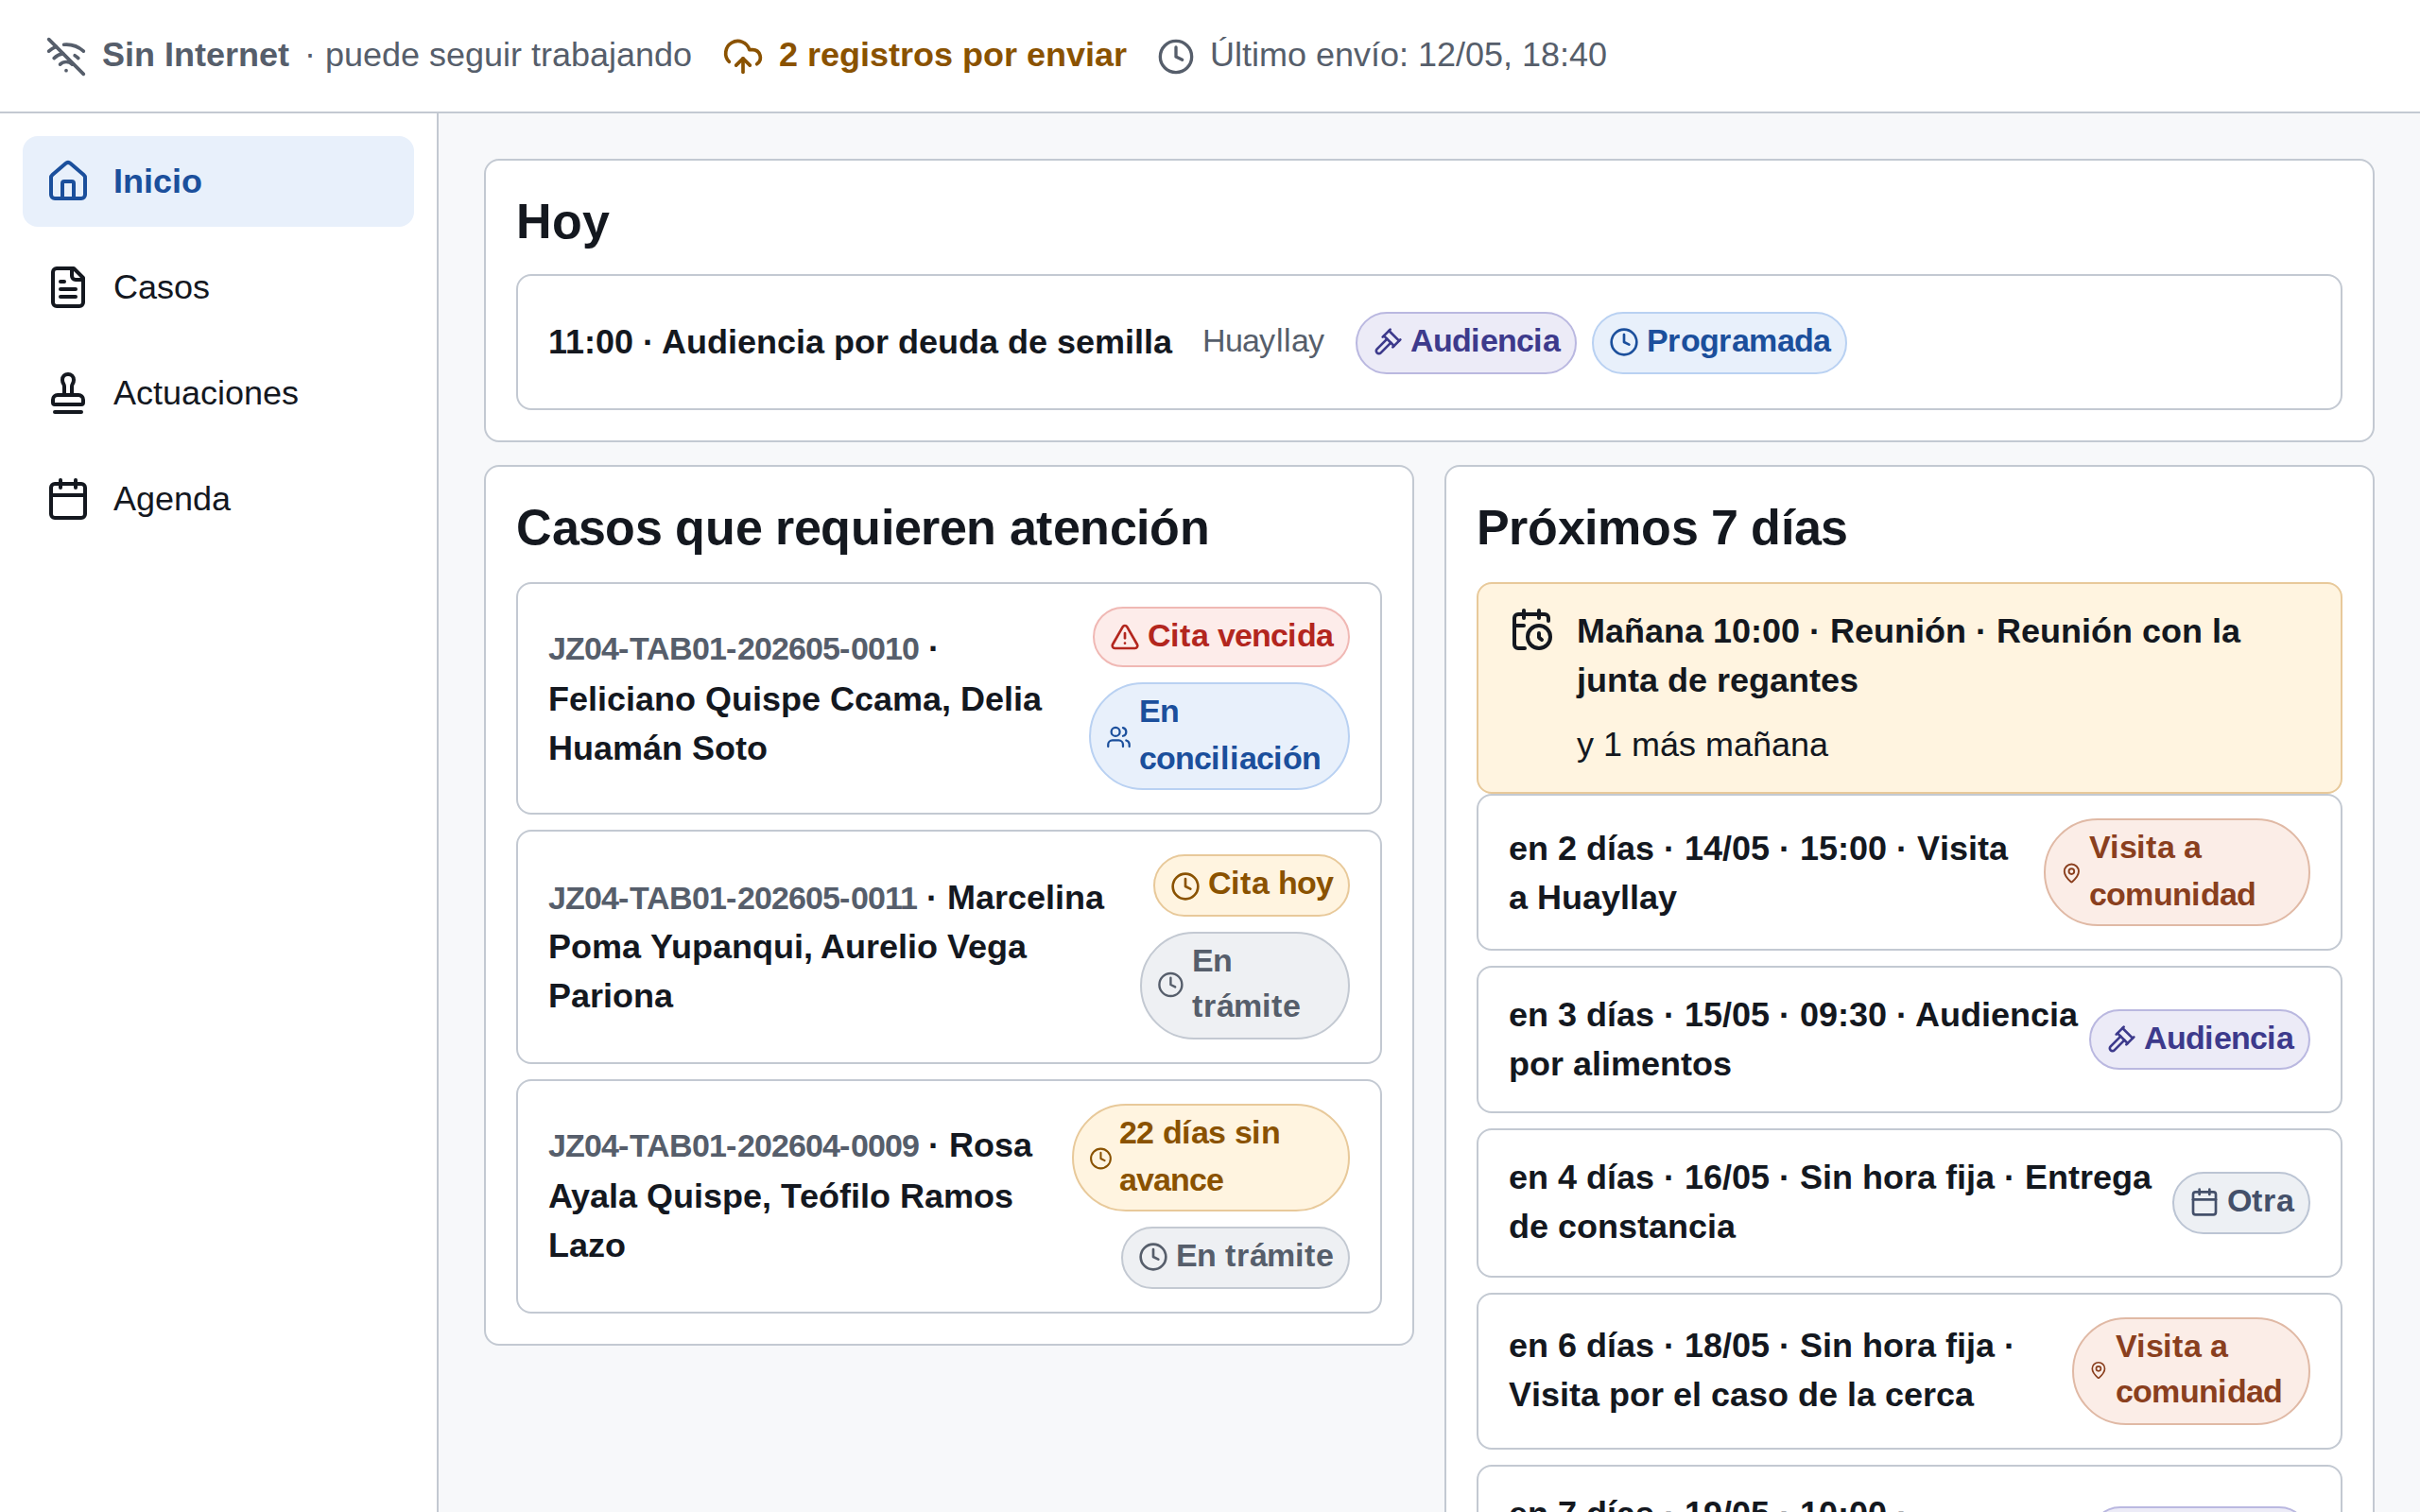
\includegraphics[width=0.82\linewidth]{capturas/F1-11_barra-pendientes.png}
\caption{P-01 · 8. Registros por enviar. El contador de la barra sube solo tras guardar sin Internet: 2 por enviar, el caso y su audiencia}
\end{figure}
\subsection{Flujo 2 · Atender un trámite, con cierre inesperado y recuperación}
\begin{figure}[H]\centering
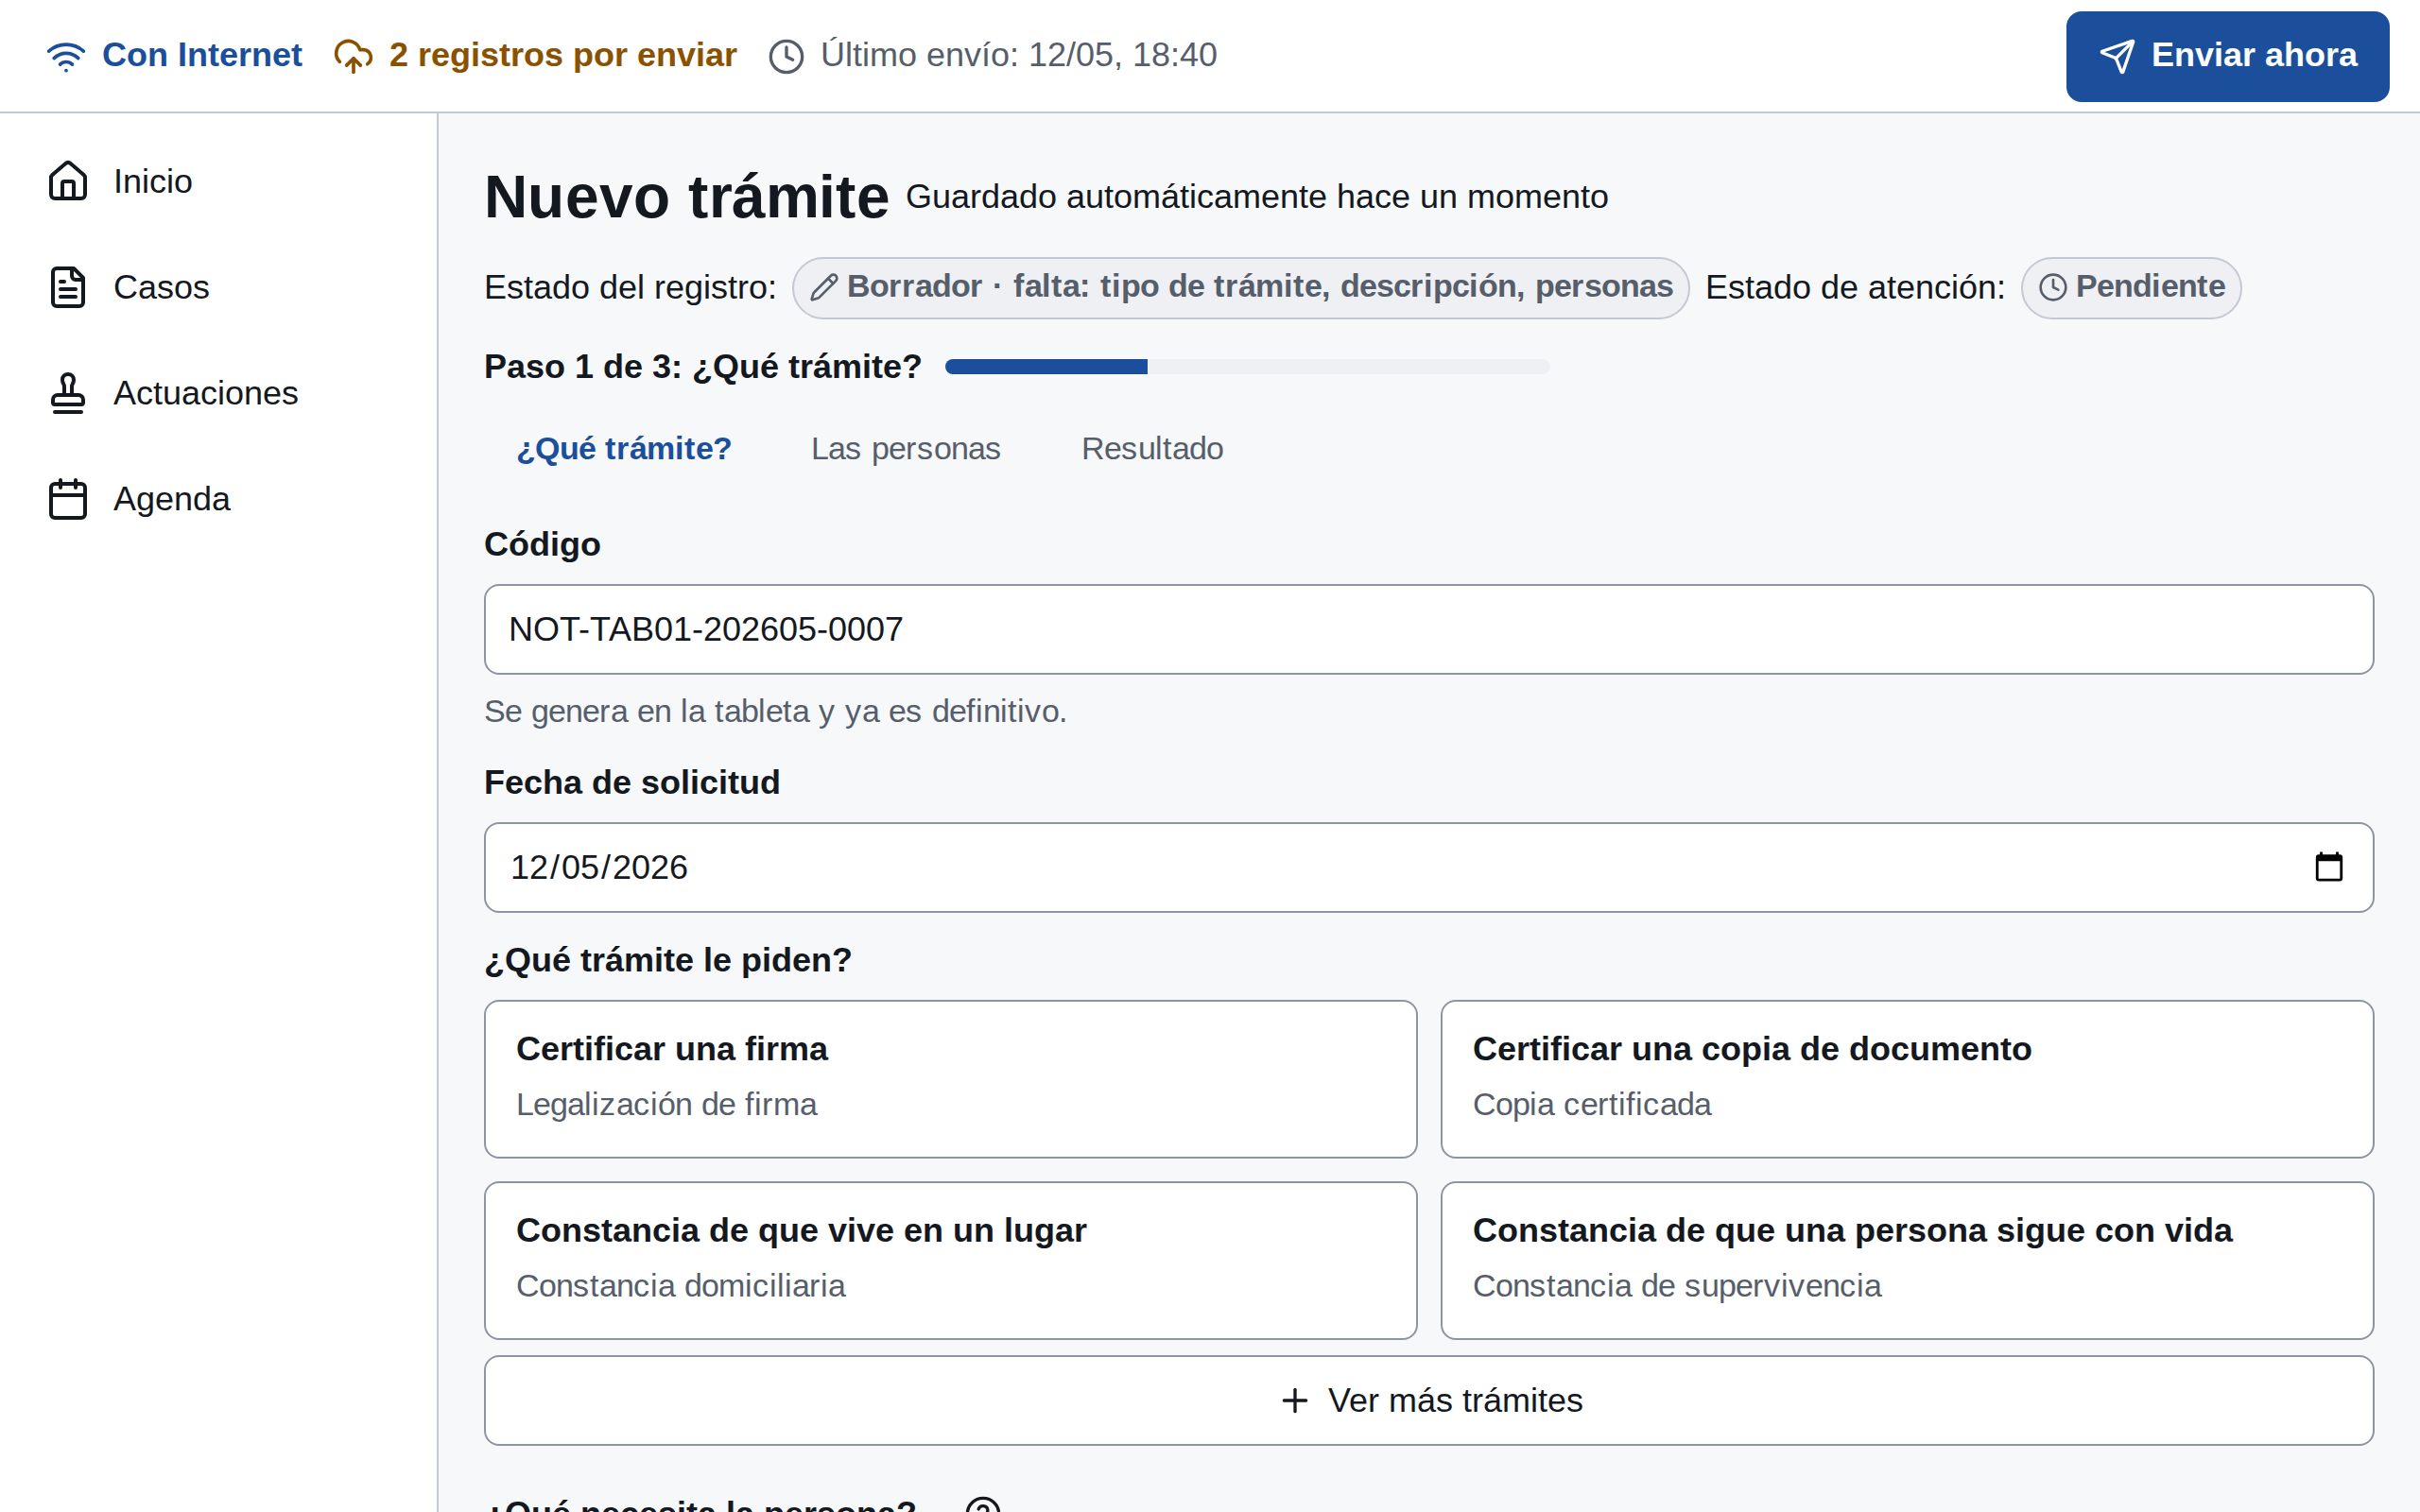
\includegraphics[width=0.82\linewidth]{capturas/F2-01_tramite-paso1.png}
\caption{P-06 · 1. Catálogo de trámites. Cuatro trámites primero, con término legal en gris, y Ver más trámites}
\end{figure}
\begin{figure}[H]\centering
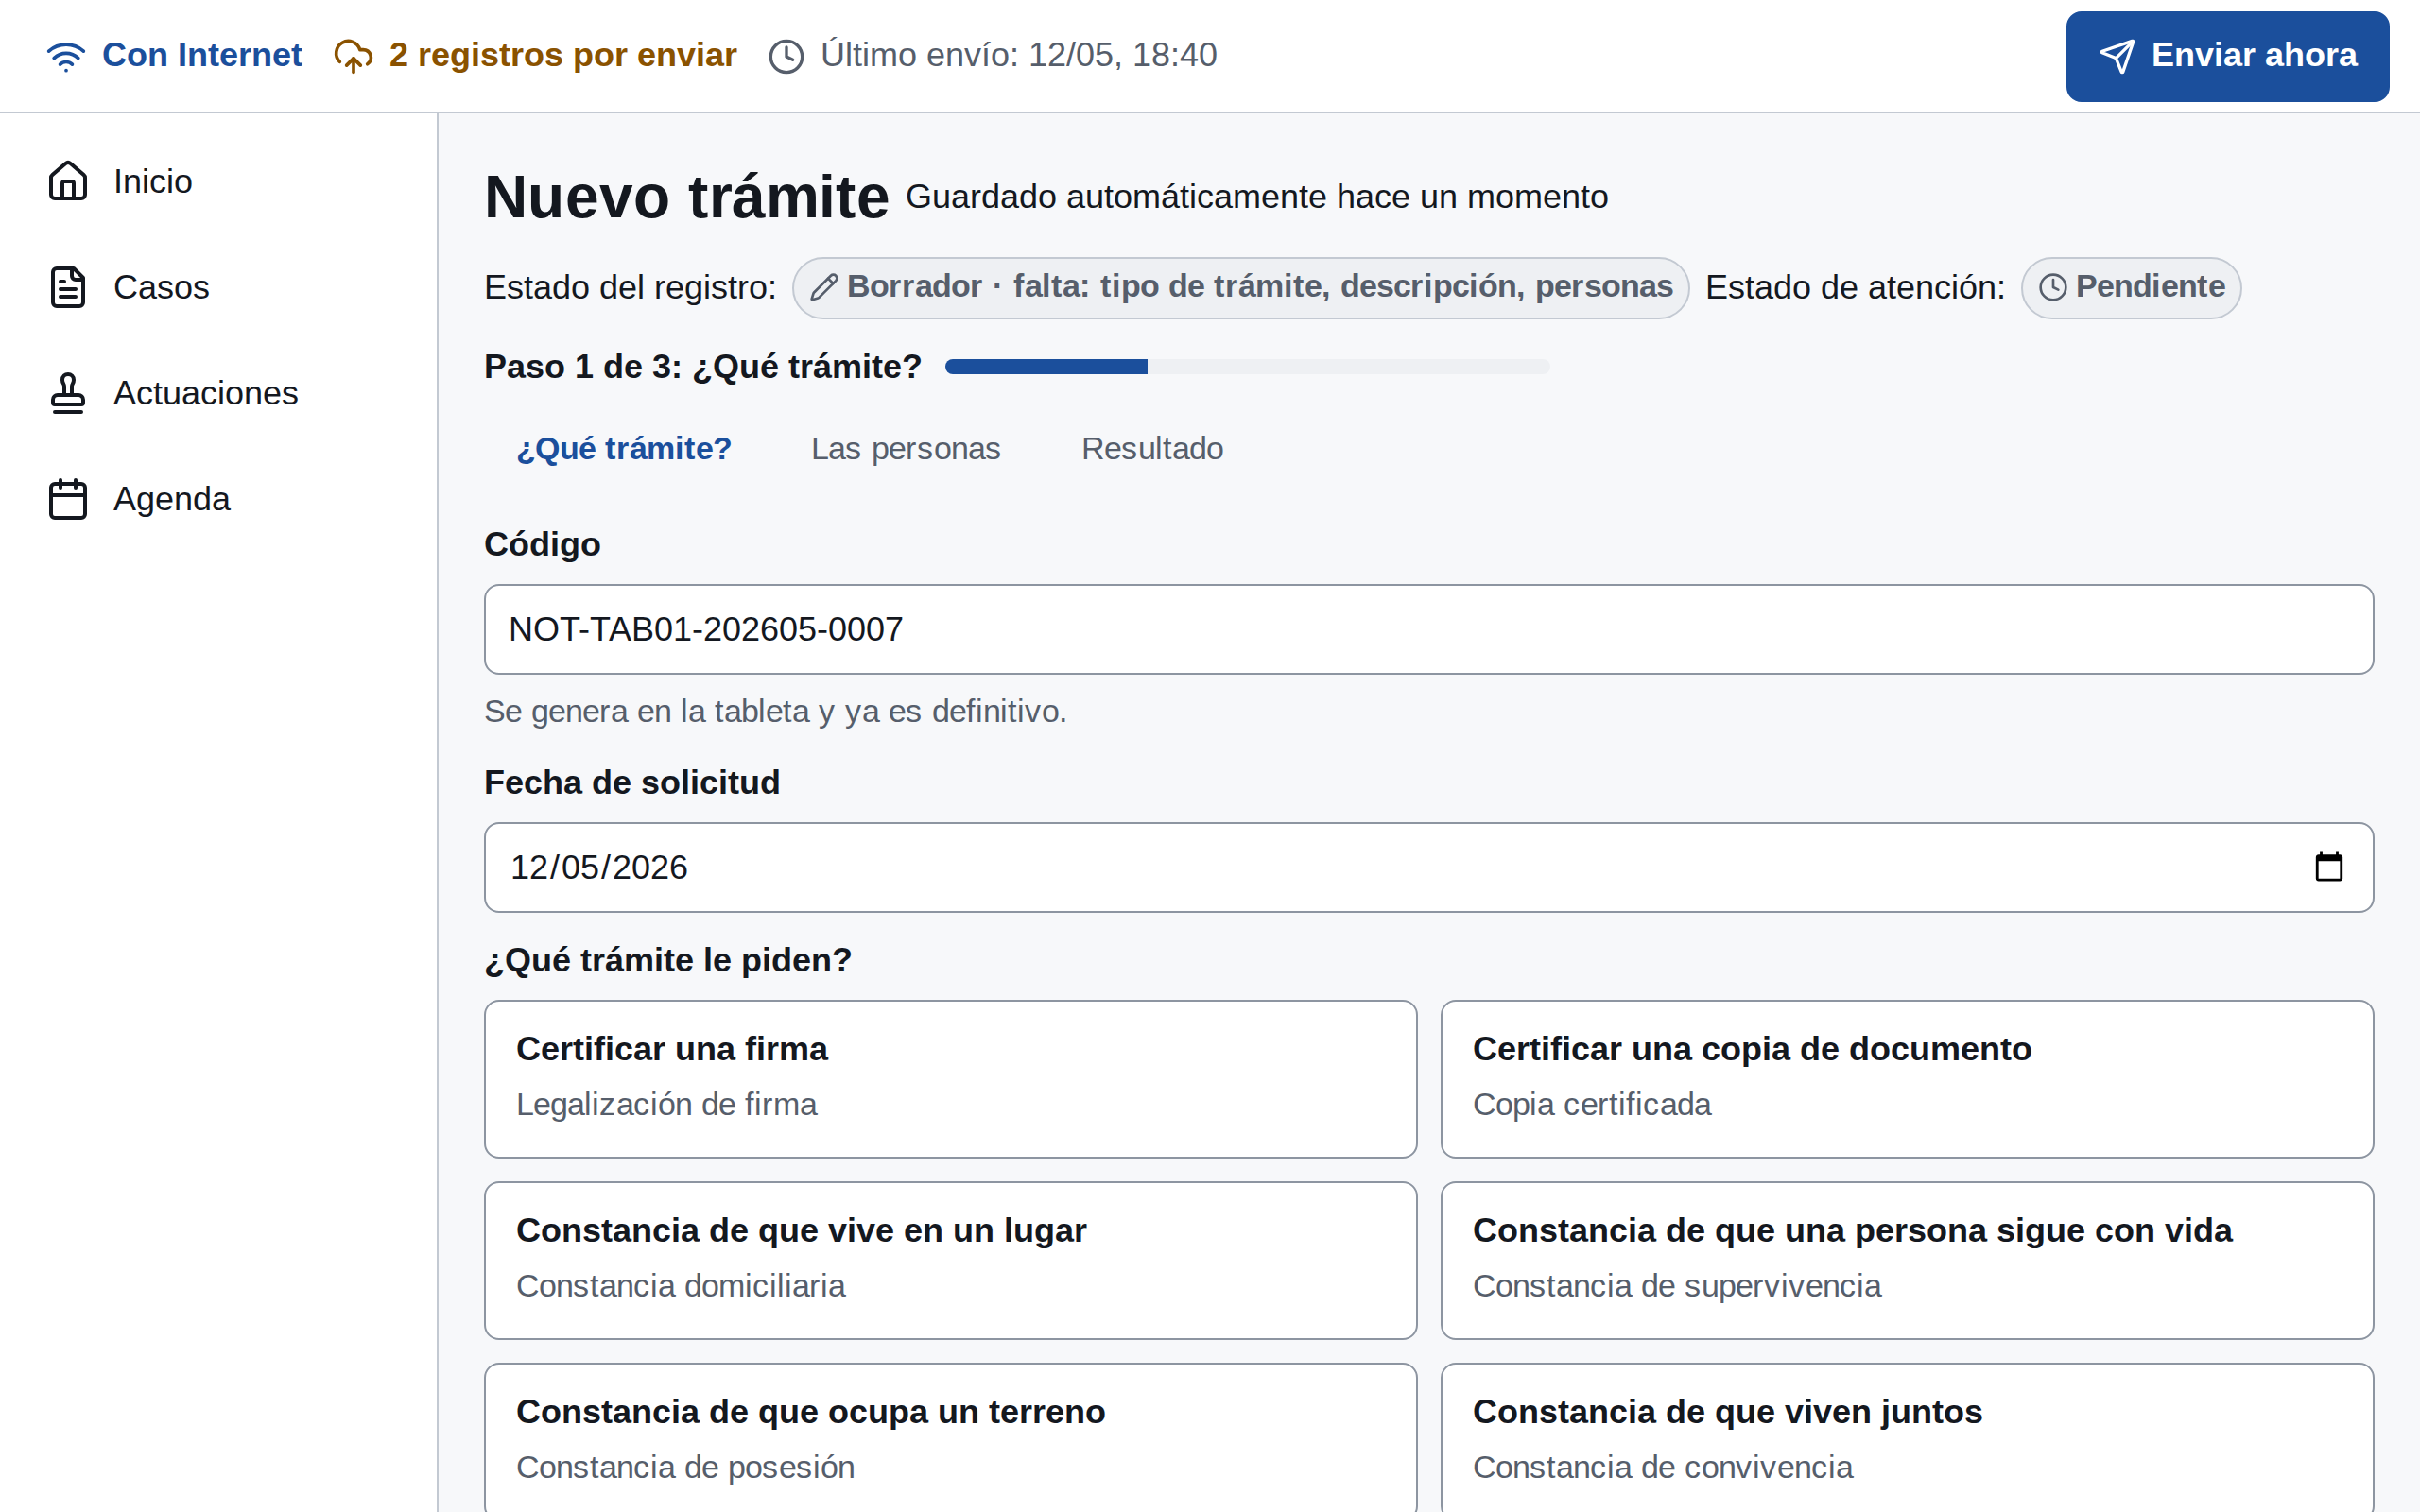
\includegraphics[width=0.82\linewidth]{capturas/F2-02_ver-mas.png}
\caption{P-06 · 1. Catálogo completo. El resto del catálogo aparece sin salir del paso}
\end{figure}
\begin{figure}[H]\centering
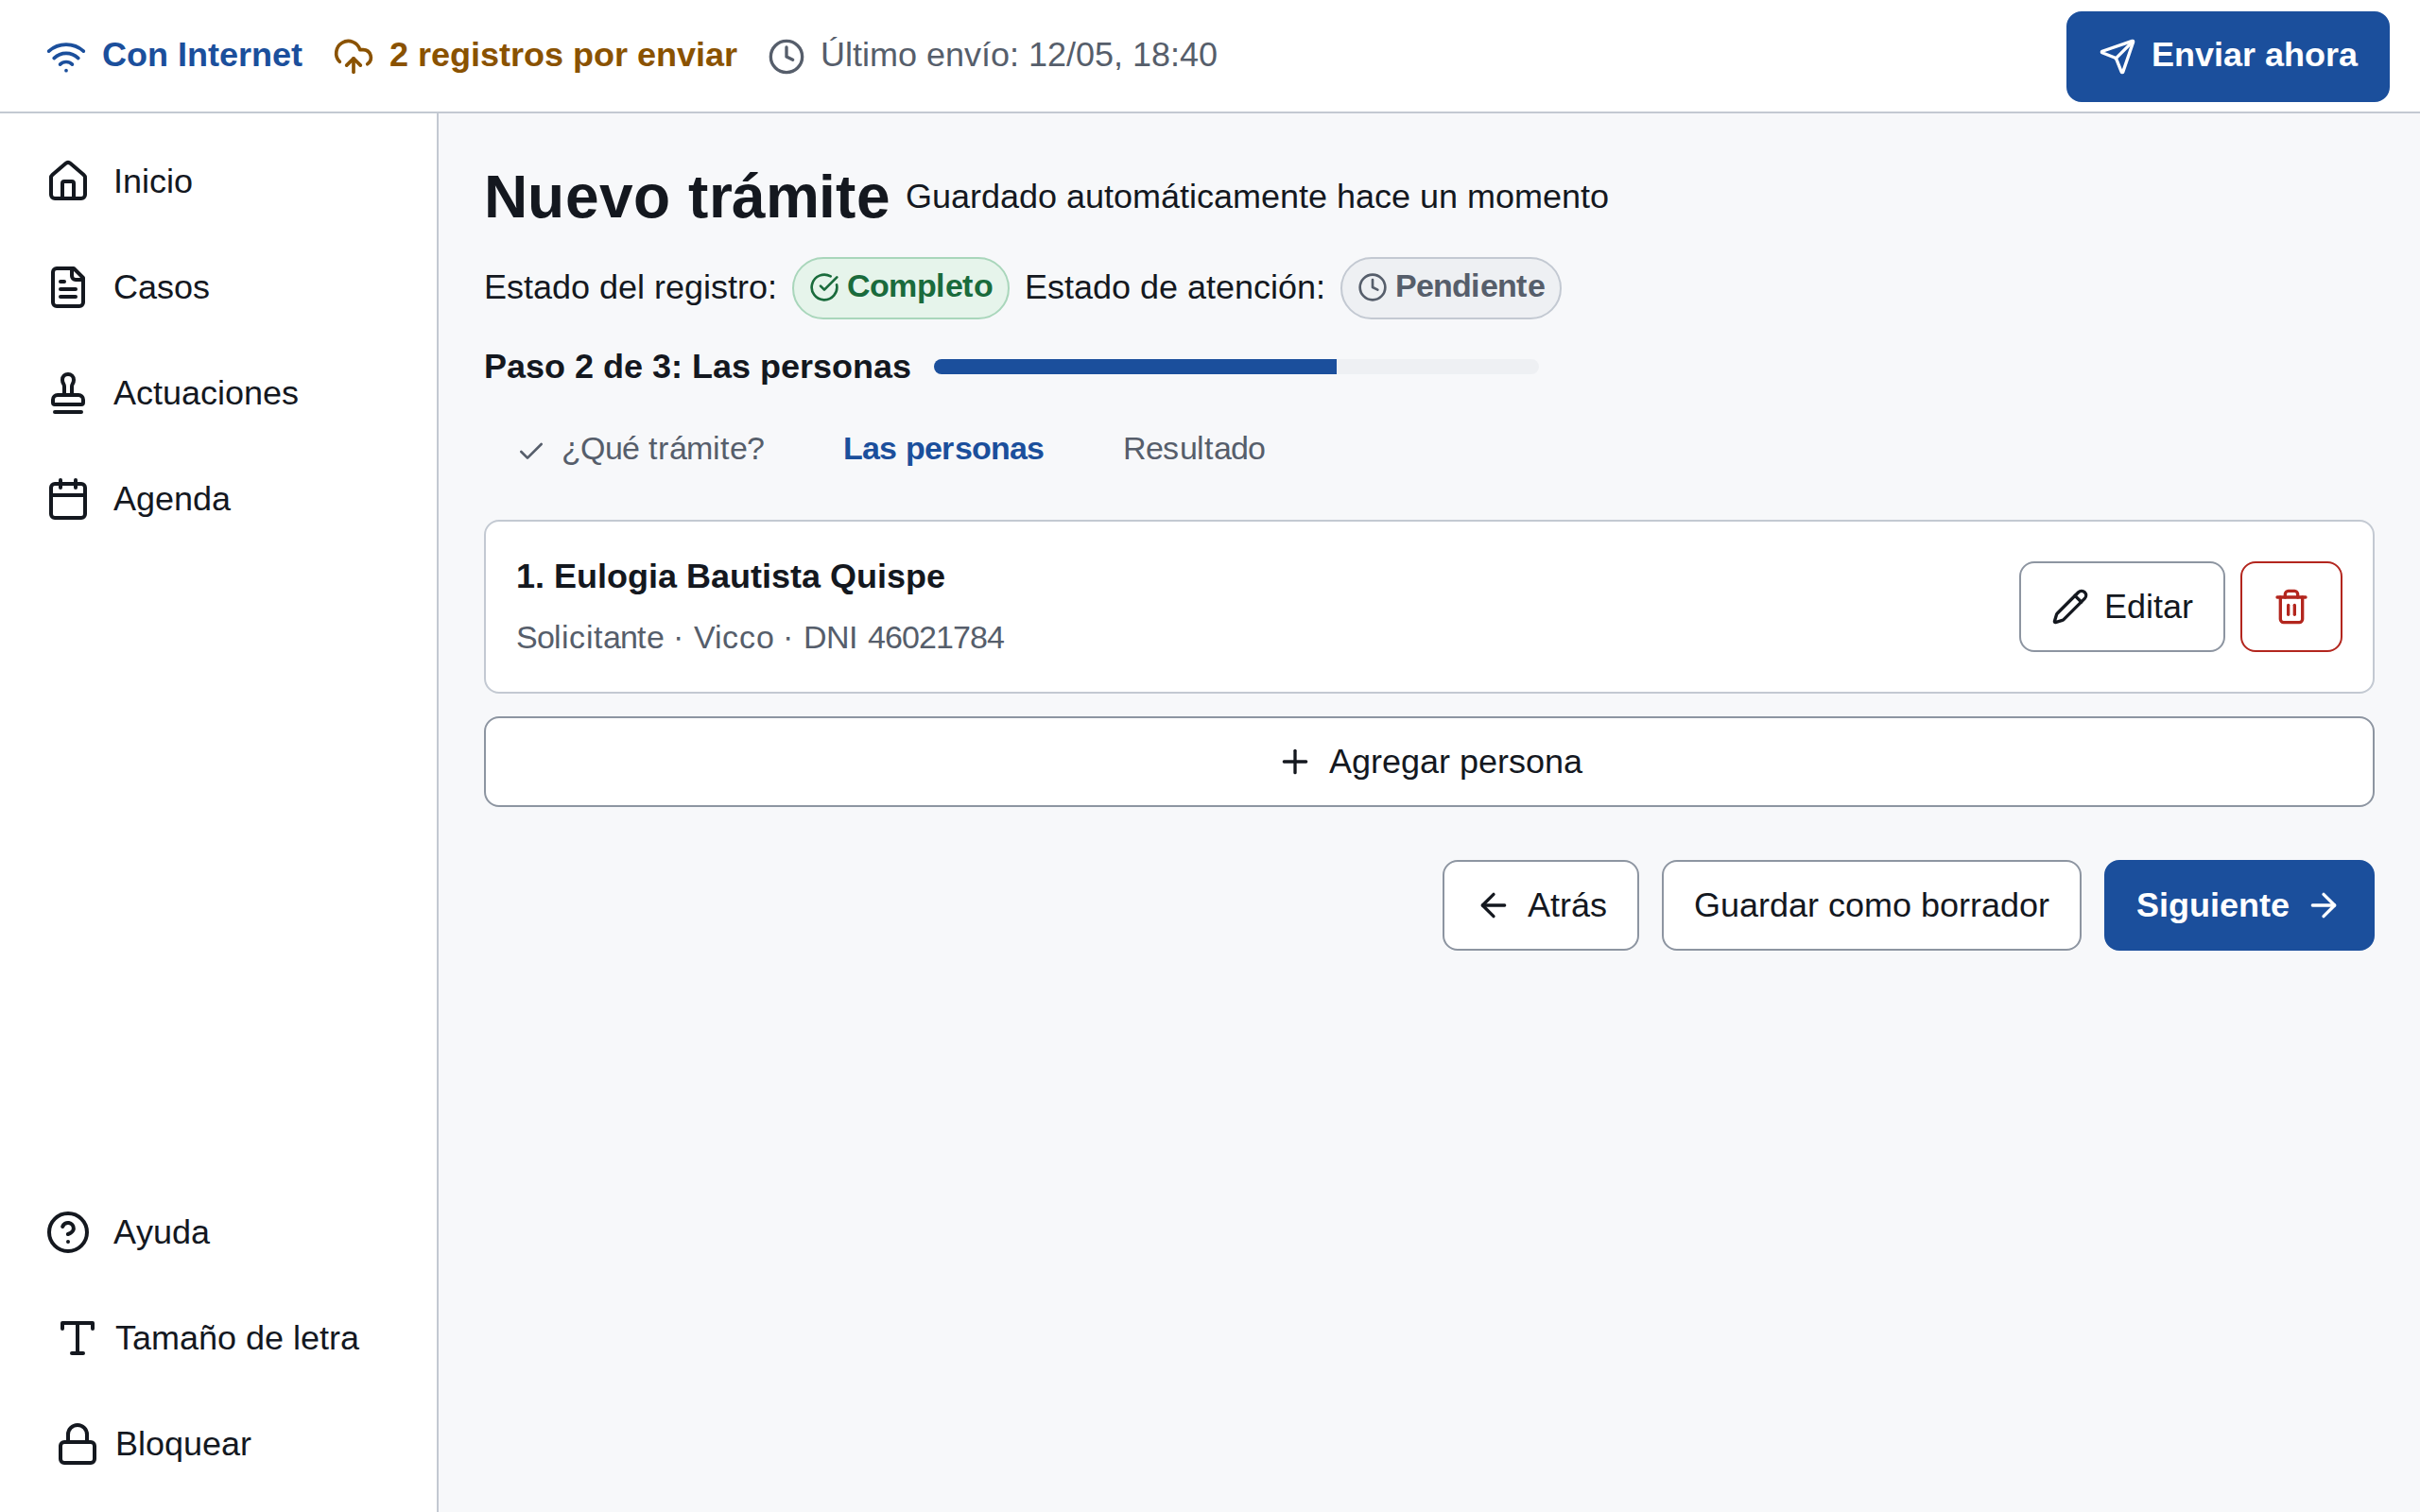
\includegraphics[width=0.82\linewidth]{capturas/F2-03_guardado-automatico.png}
\caption{P-06 · 2. Guardado automático. El texto discreto avisa que lo escrito ya está guardado en la tableta}
\end{figure}
\begin{figure}[H]\centering
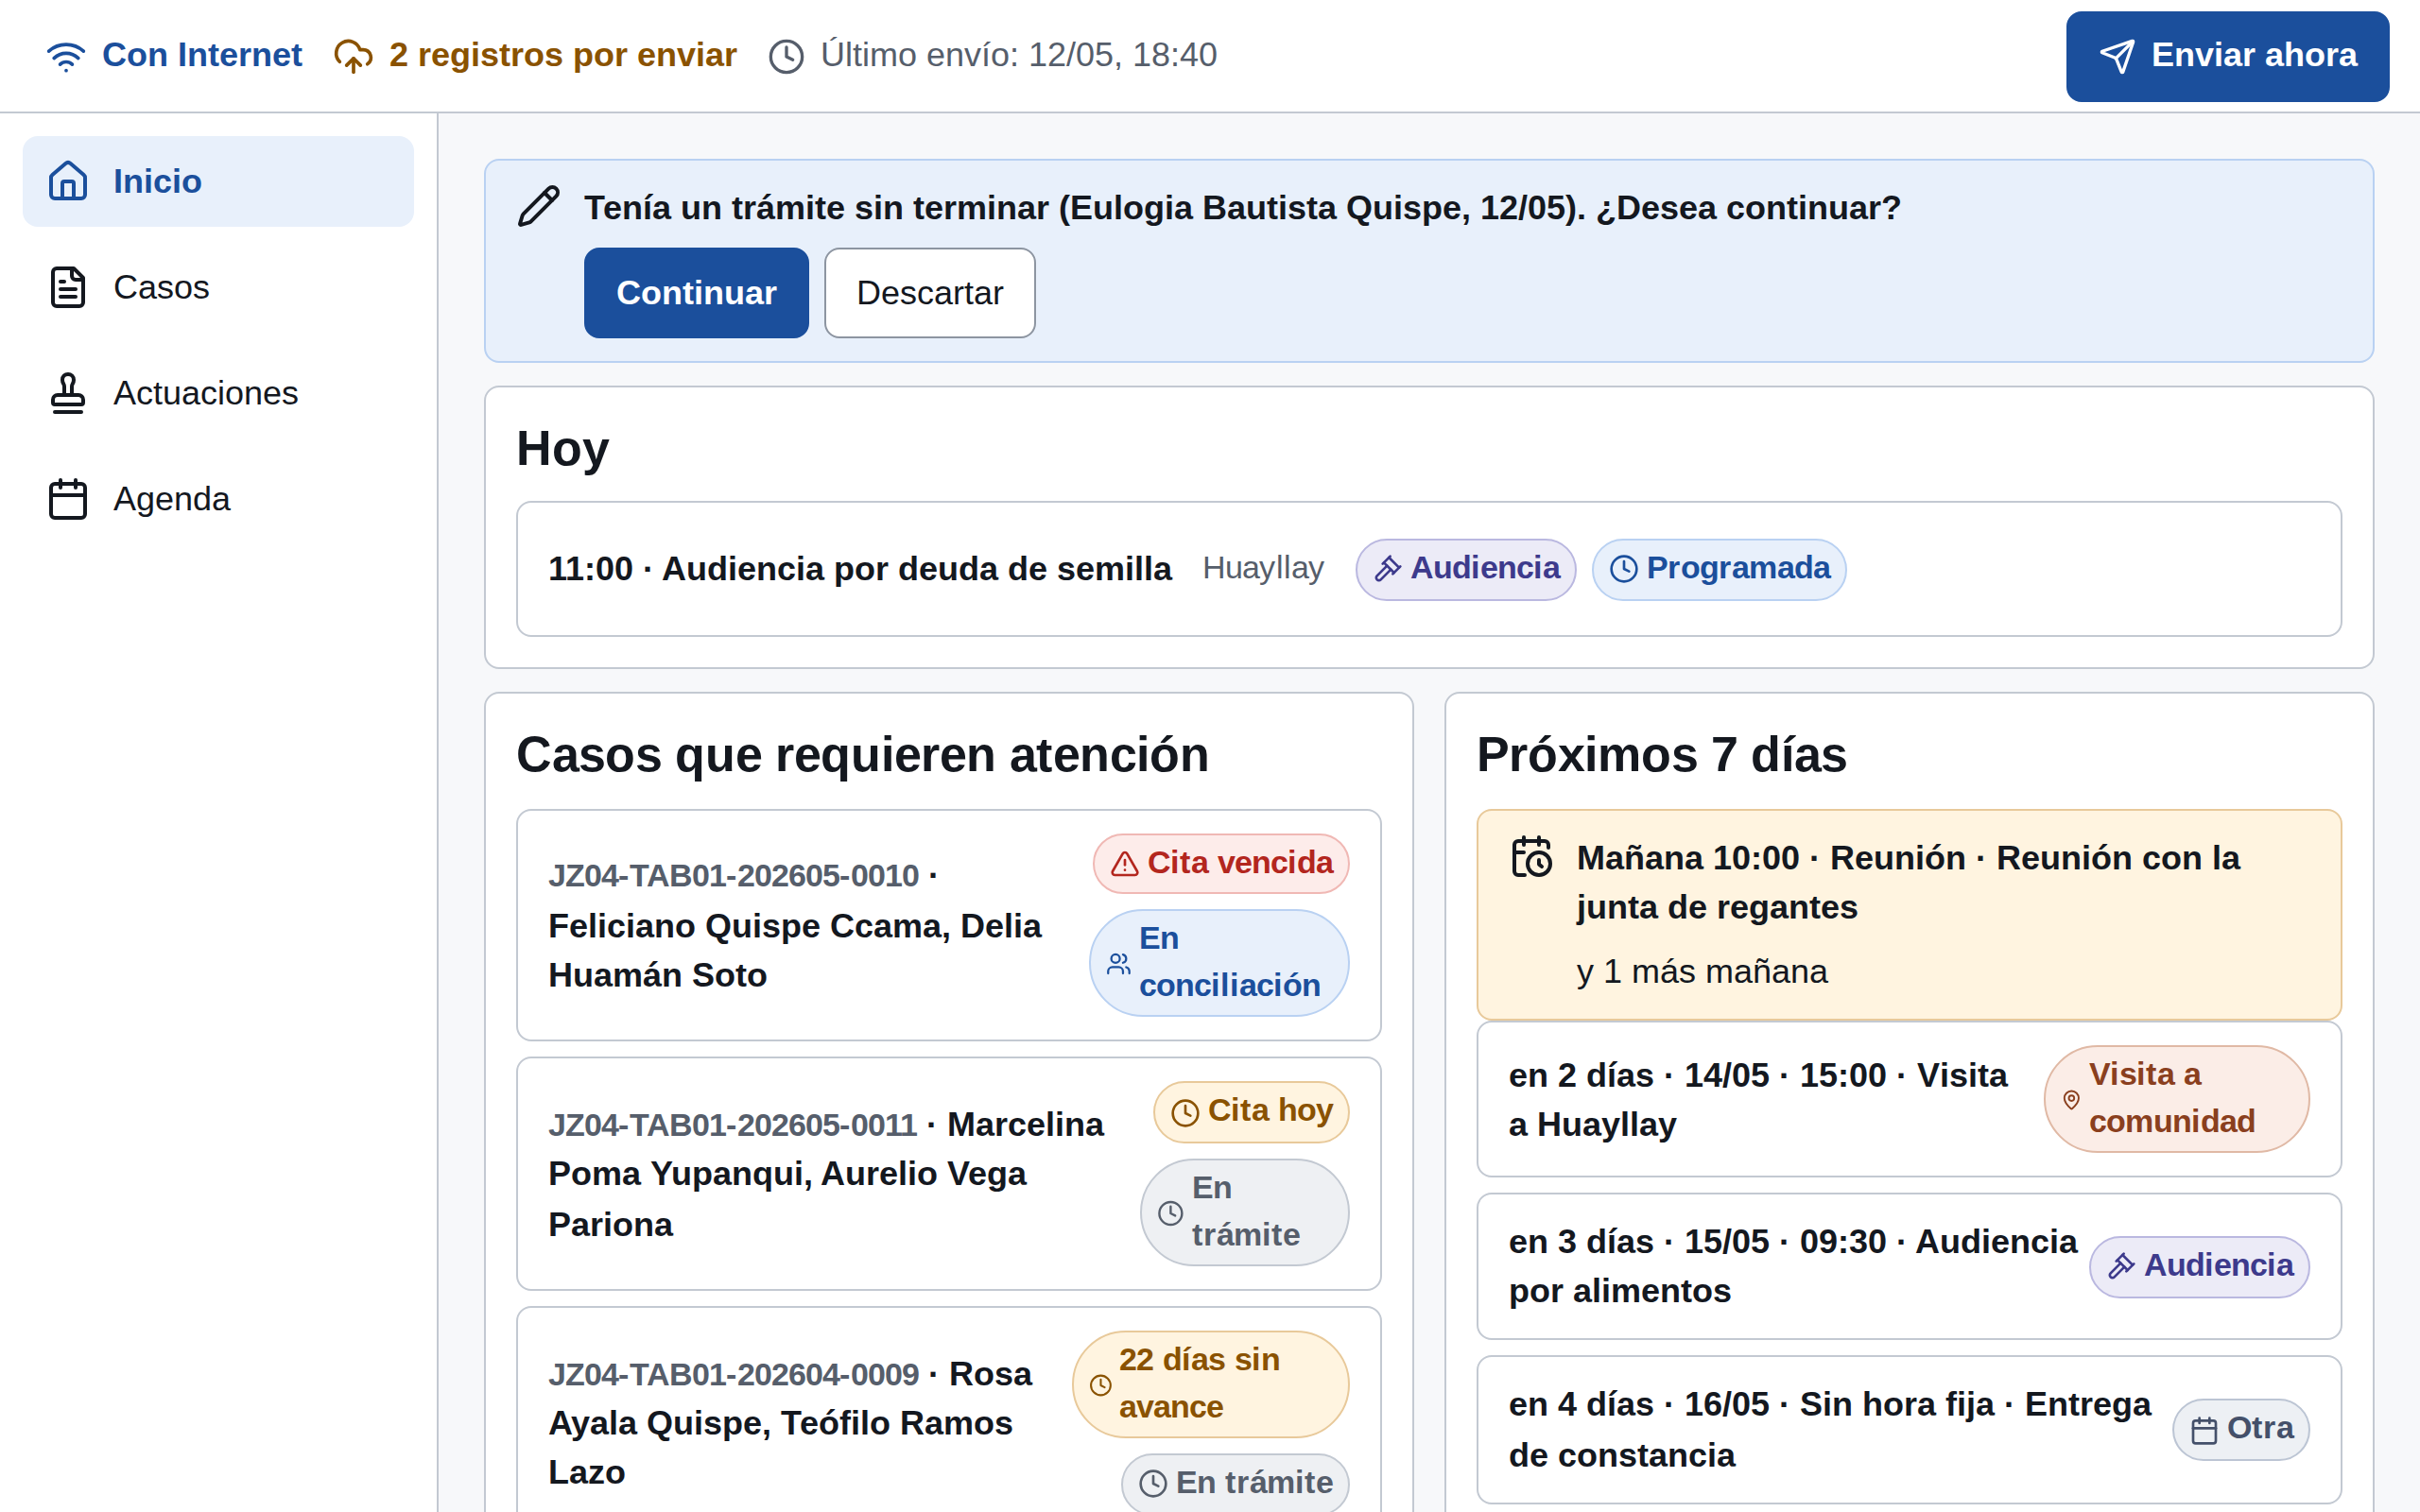
\includegraphics[width=0.82\linewidth]{capturas/F2-04_recuperacion.png}
\caption{P-01 · 3. La aplicación se cerró y se recupera. Al volver, ofrece continuar el trámite sin terminar en vez de perderlo}
\end{figure}
\begin{figure}[H]\centering
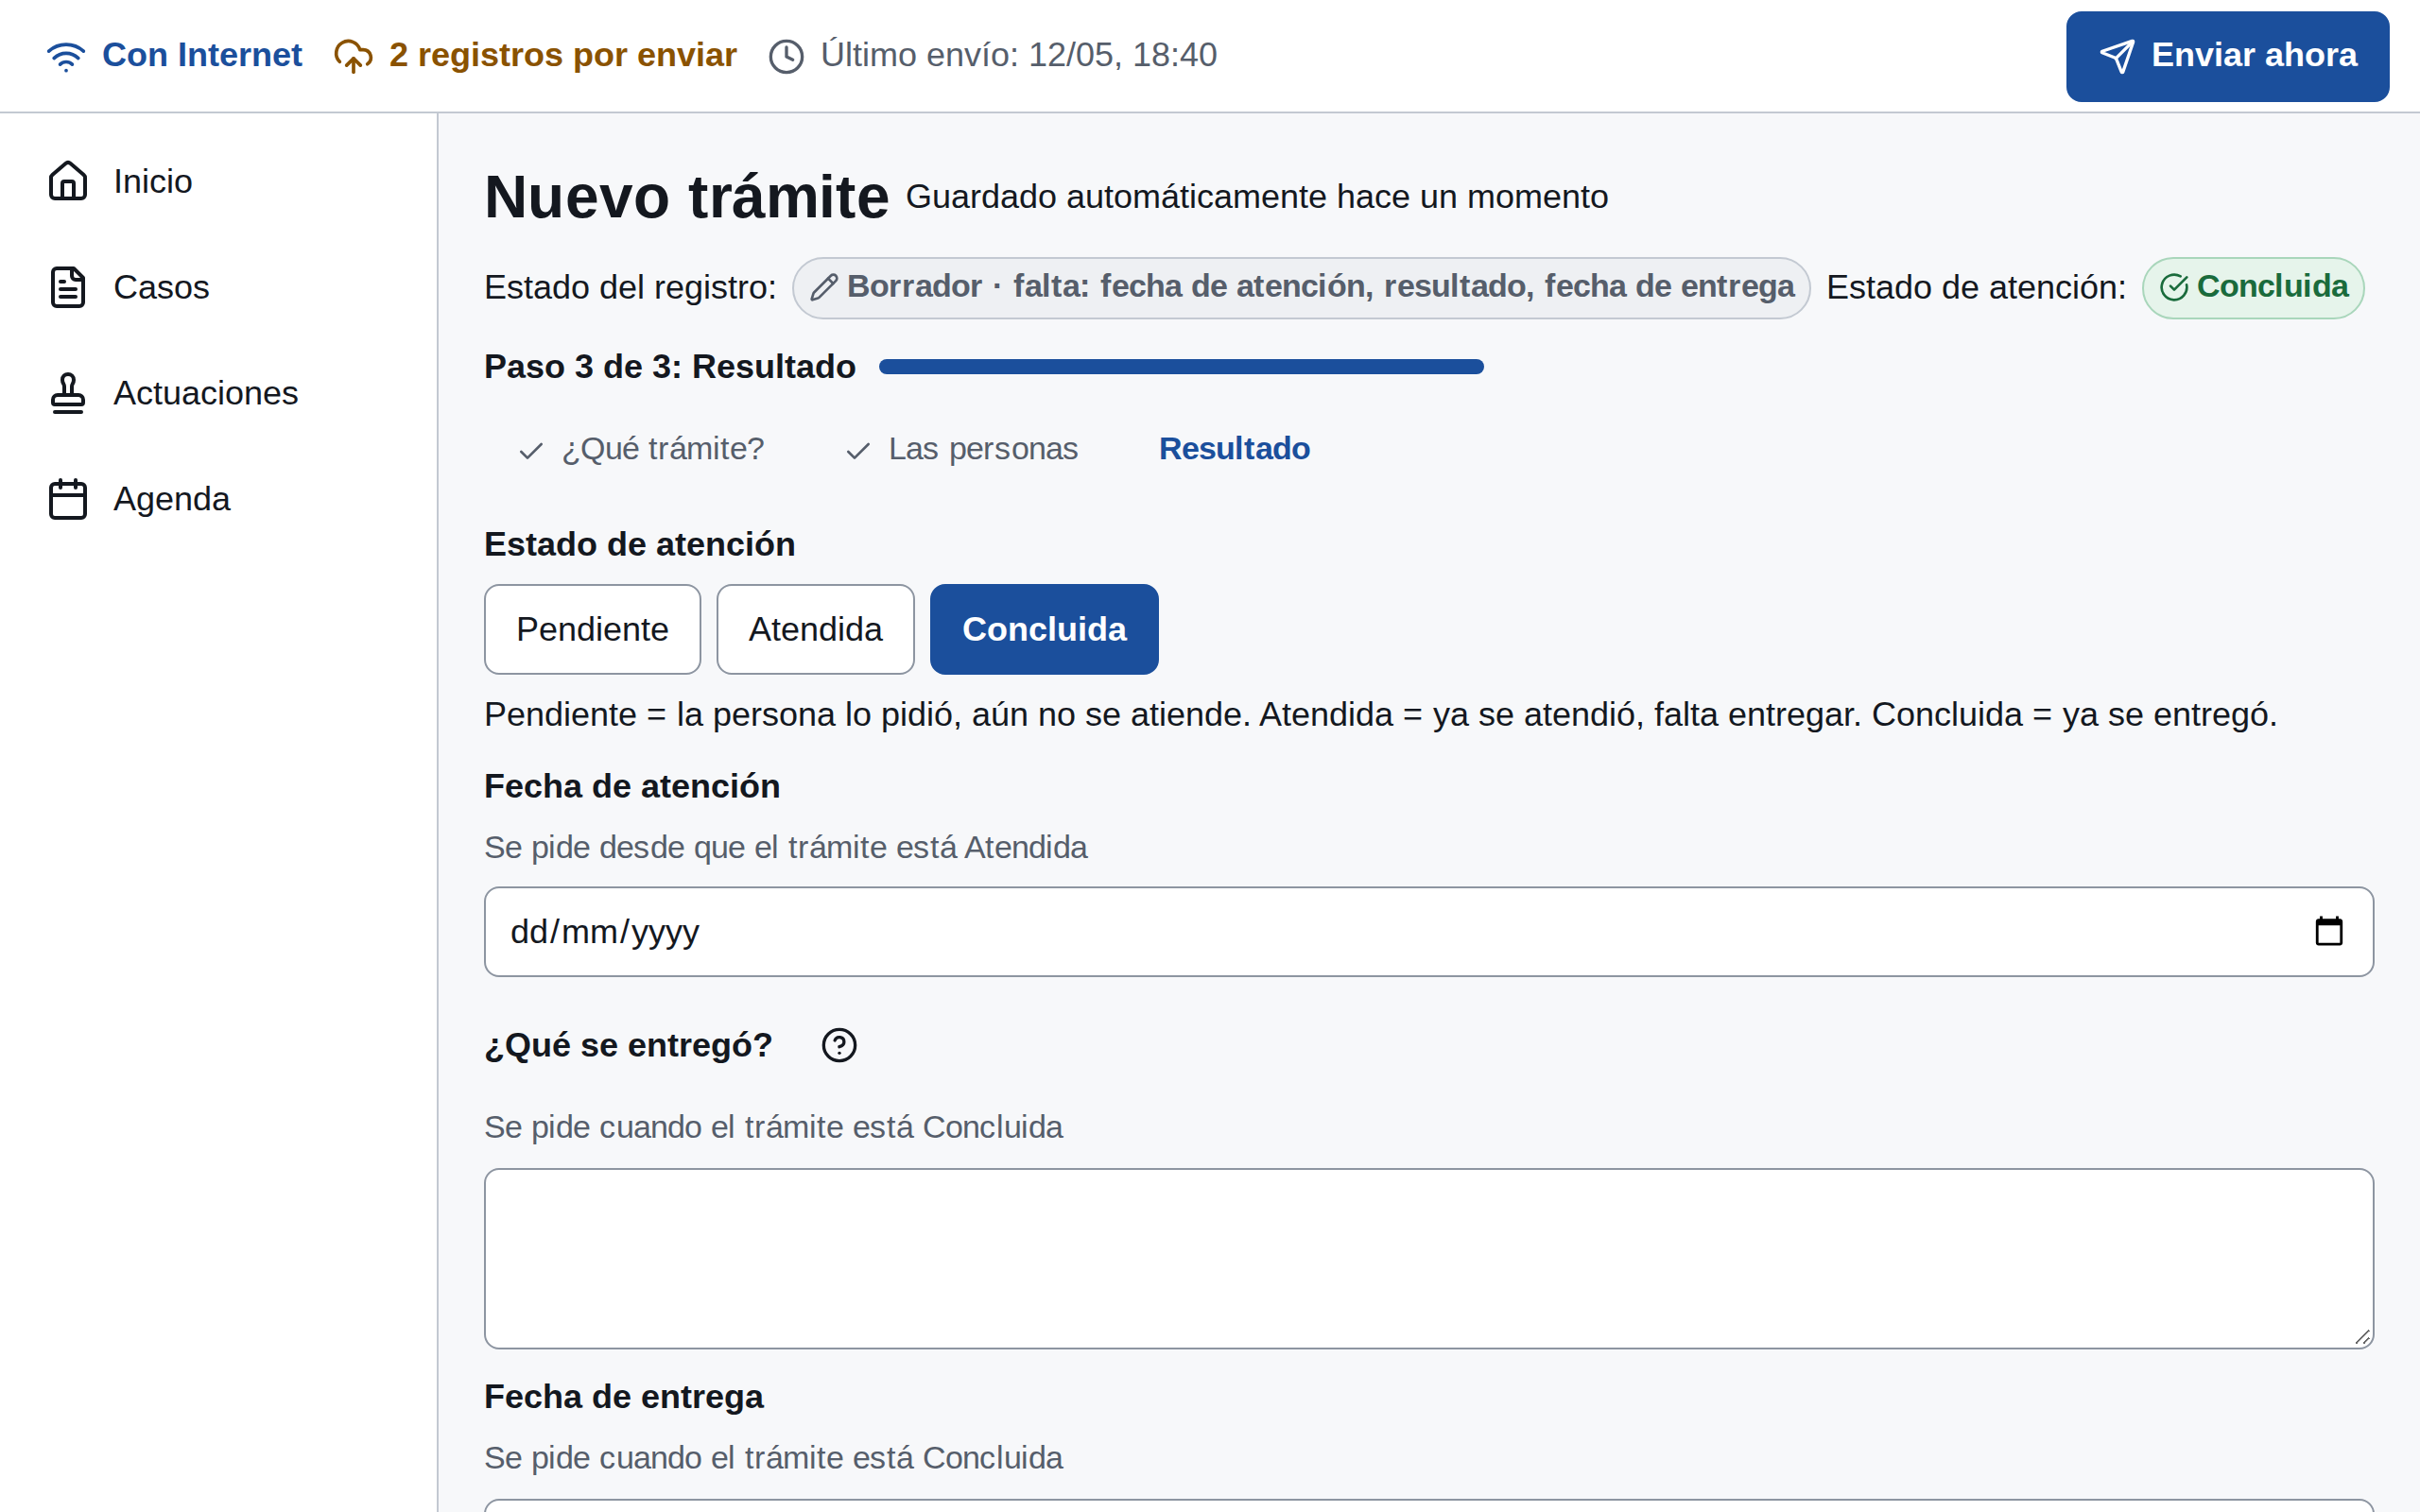
\includegraphics[width=0.82\linewidth]{capturas/F2-05_condicionales.png}
\caption{P-06 · 4. Campos condicionales. Al pasar a Concluida aparecen los campos que se piden, con su línea explicativa}
\end{figure}
\begin{figure}[H]\centering
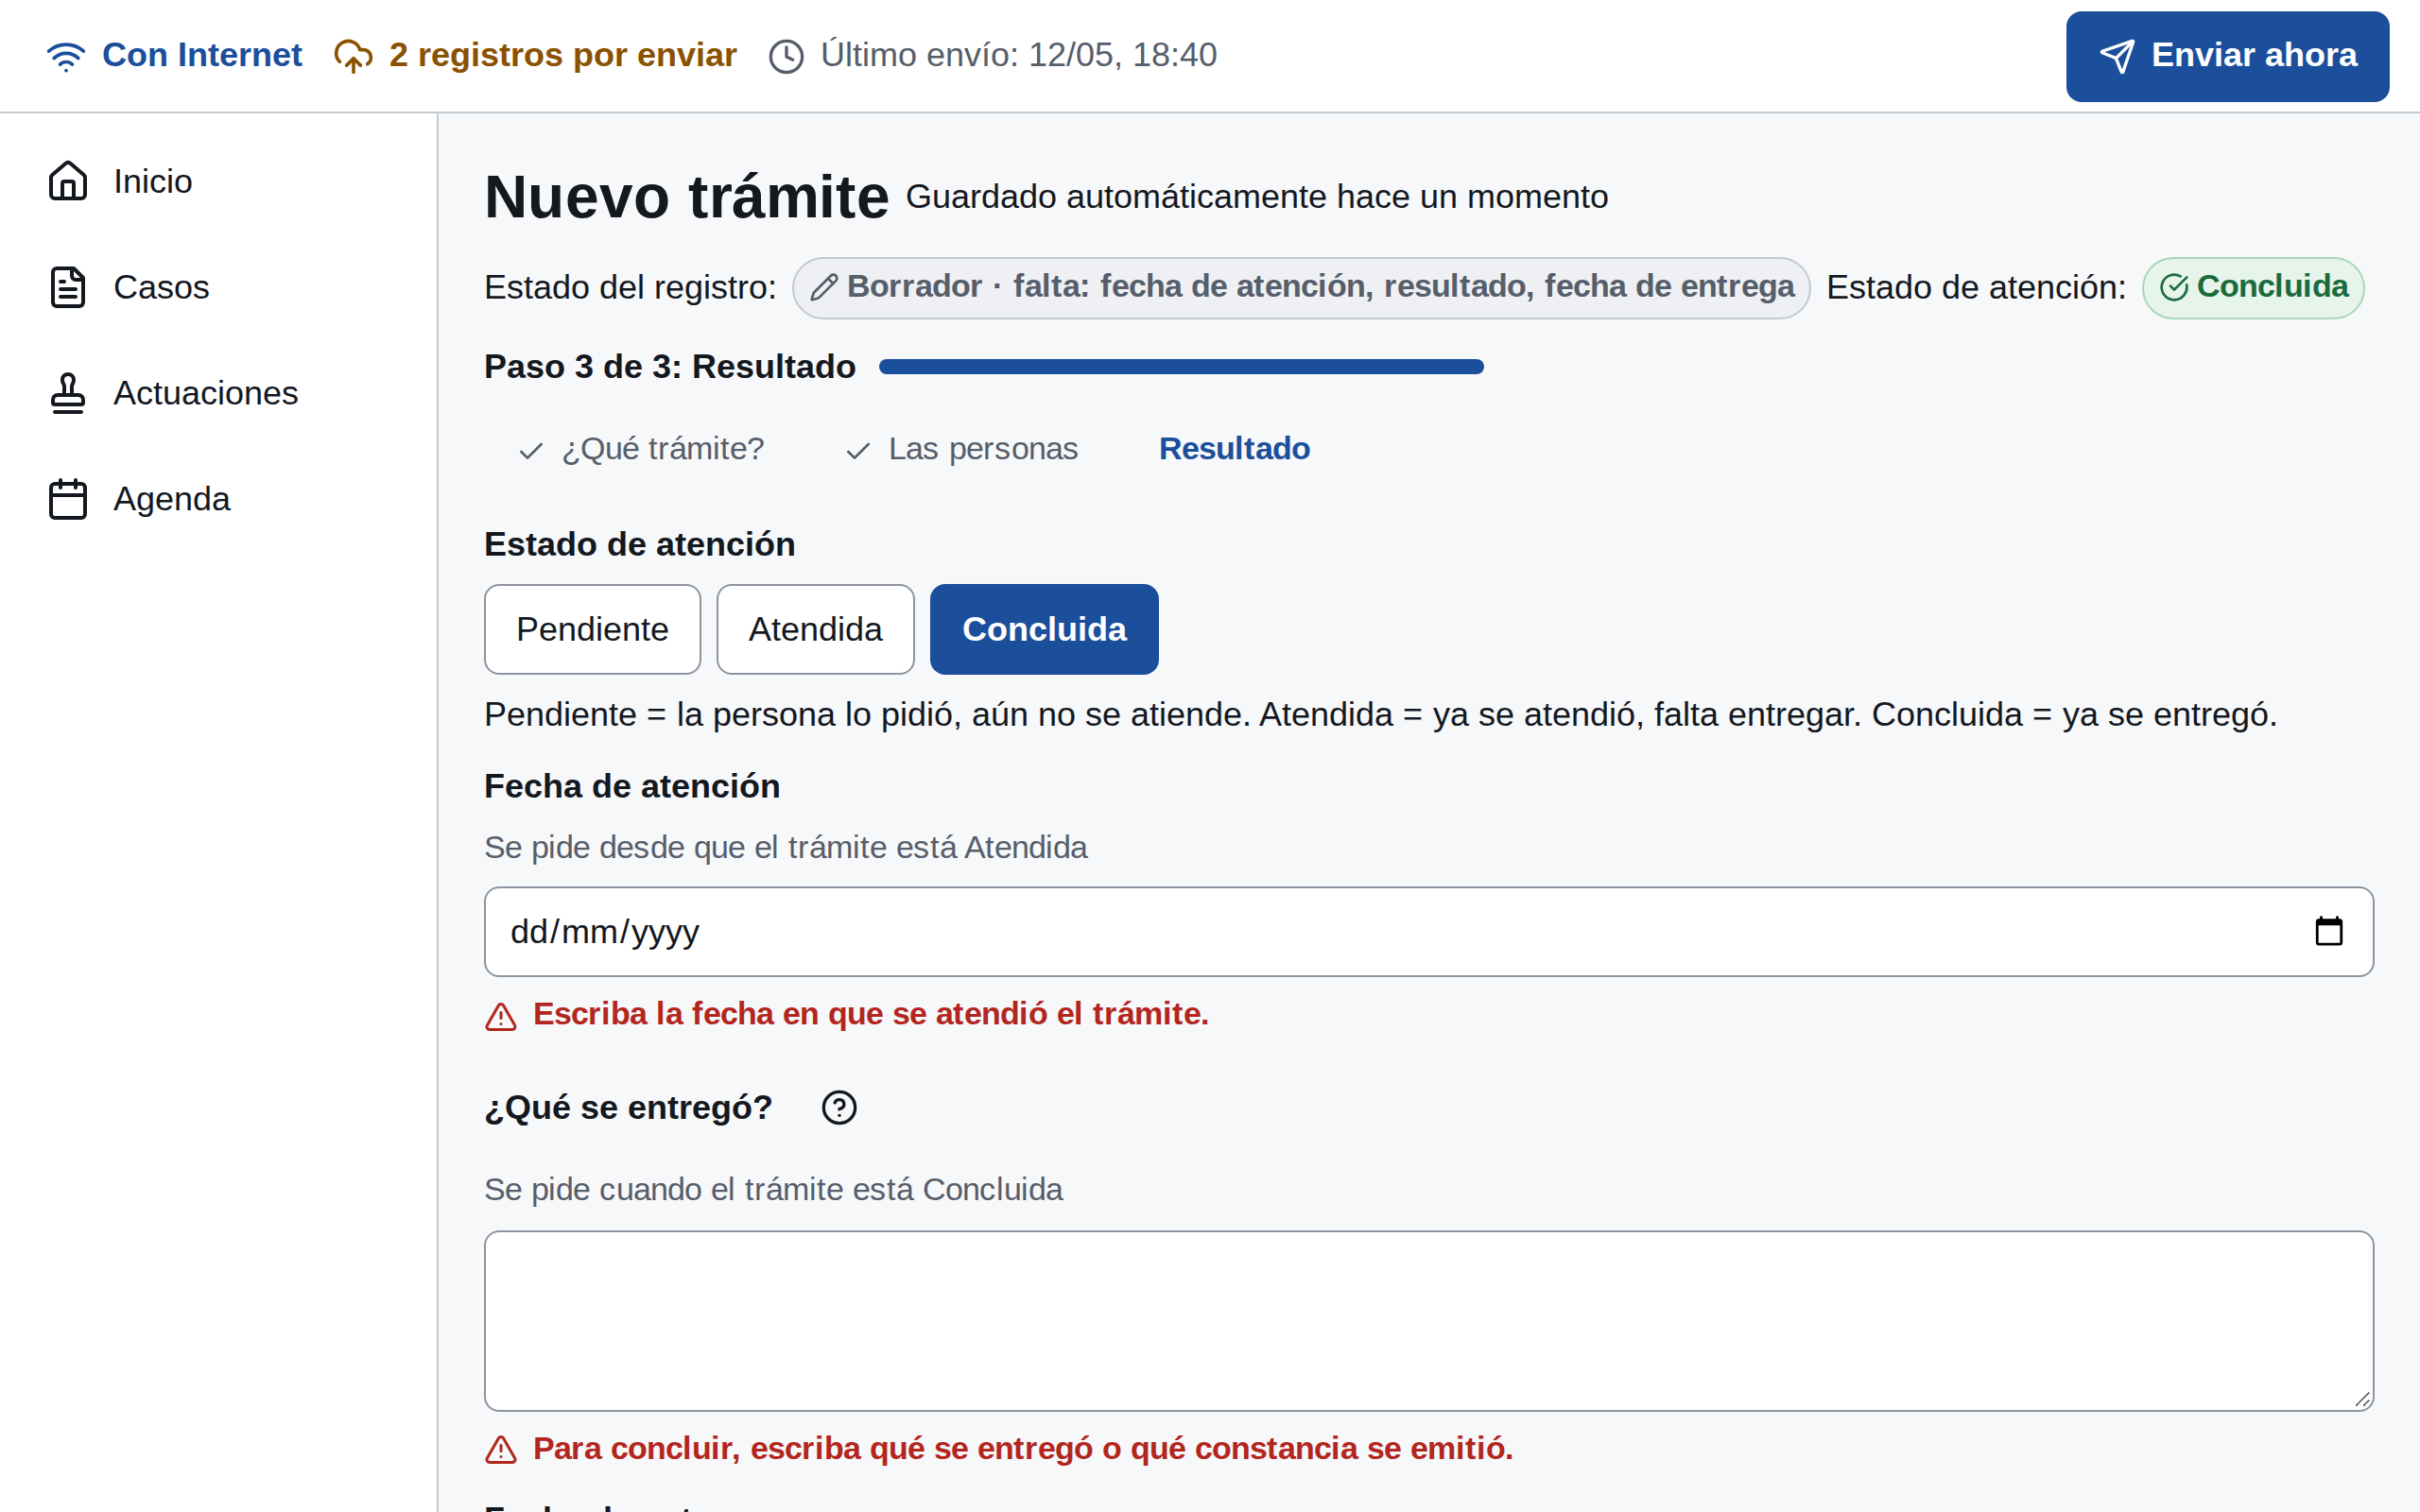
\includegraphics[width=0.82\linewidth]{capturas/F2-06_error-condicional.png}
\caption{P-06 · 4. Error de campo condicional. No deja concluir sin decir qué se entregó, y lo explica en una frase}
\end{figure}
\begin{figure}[H]\centering
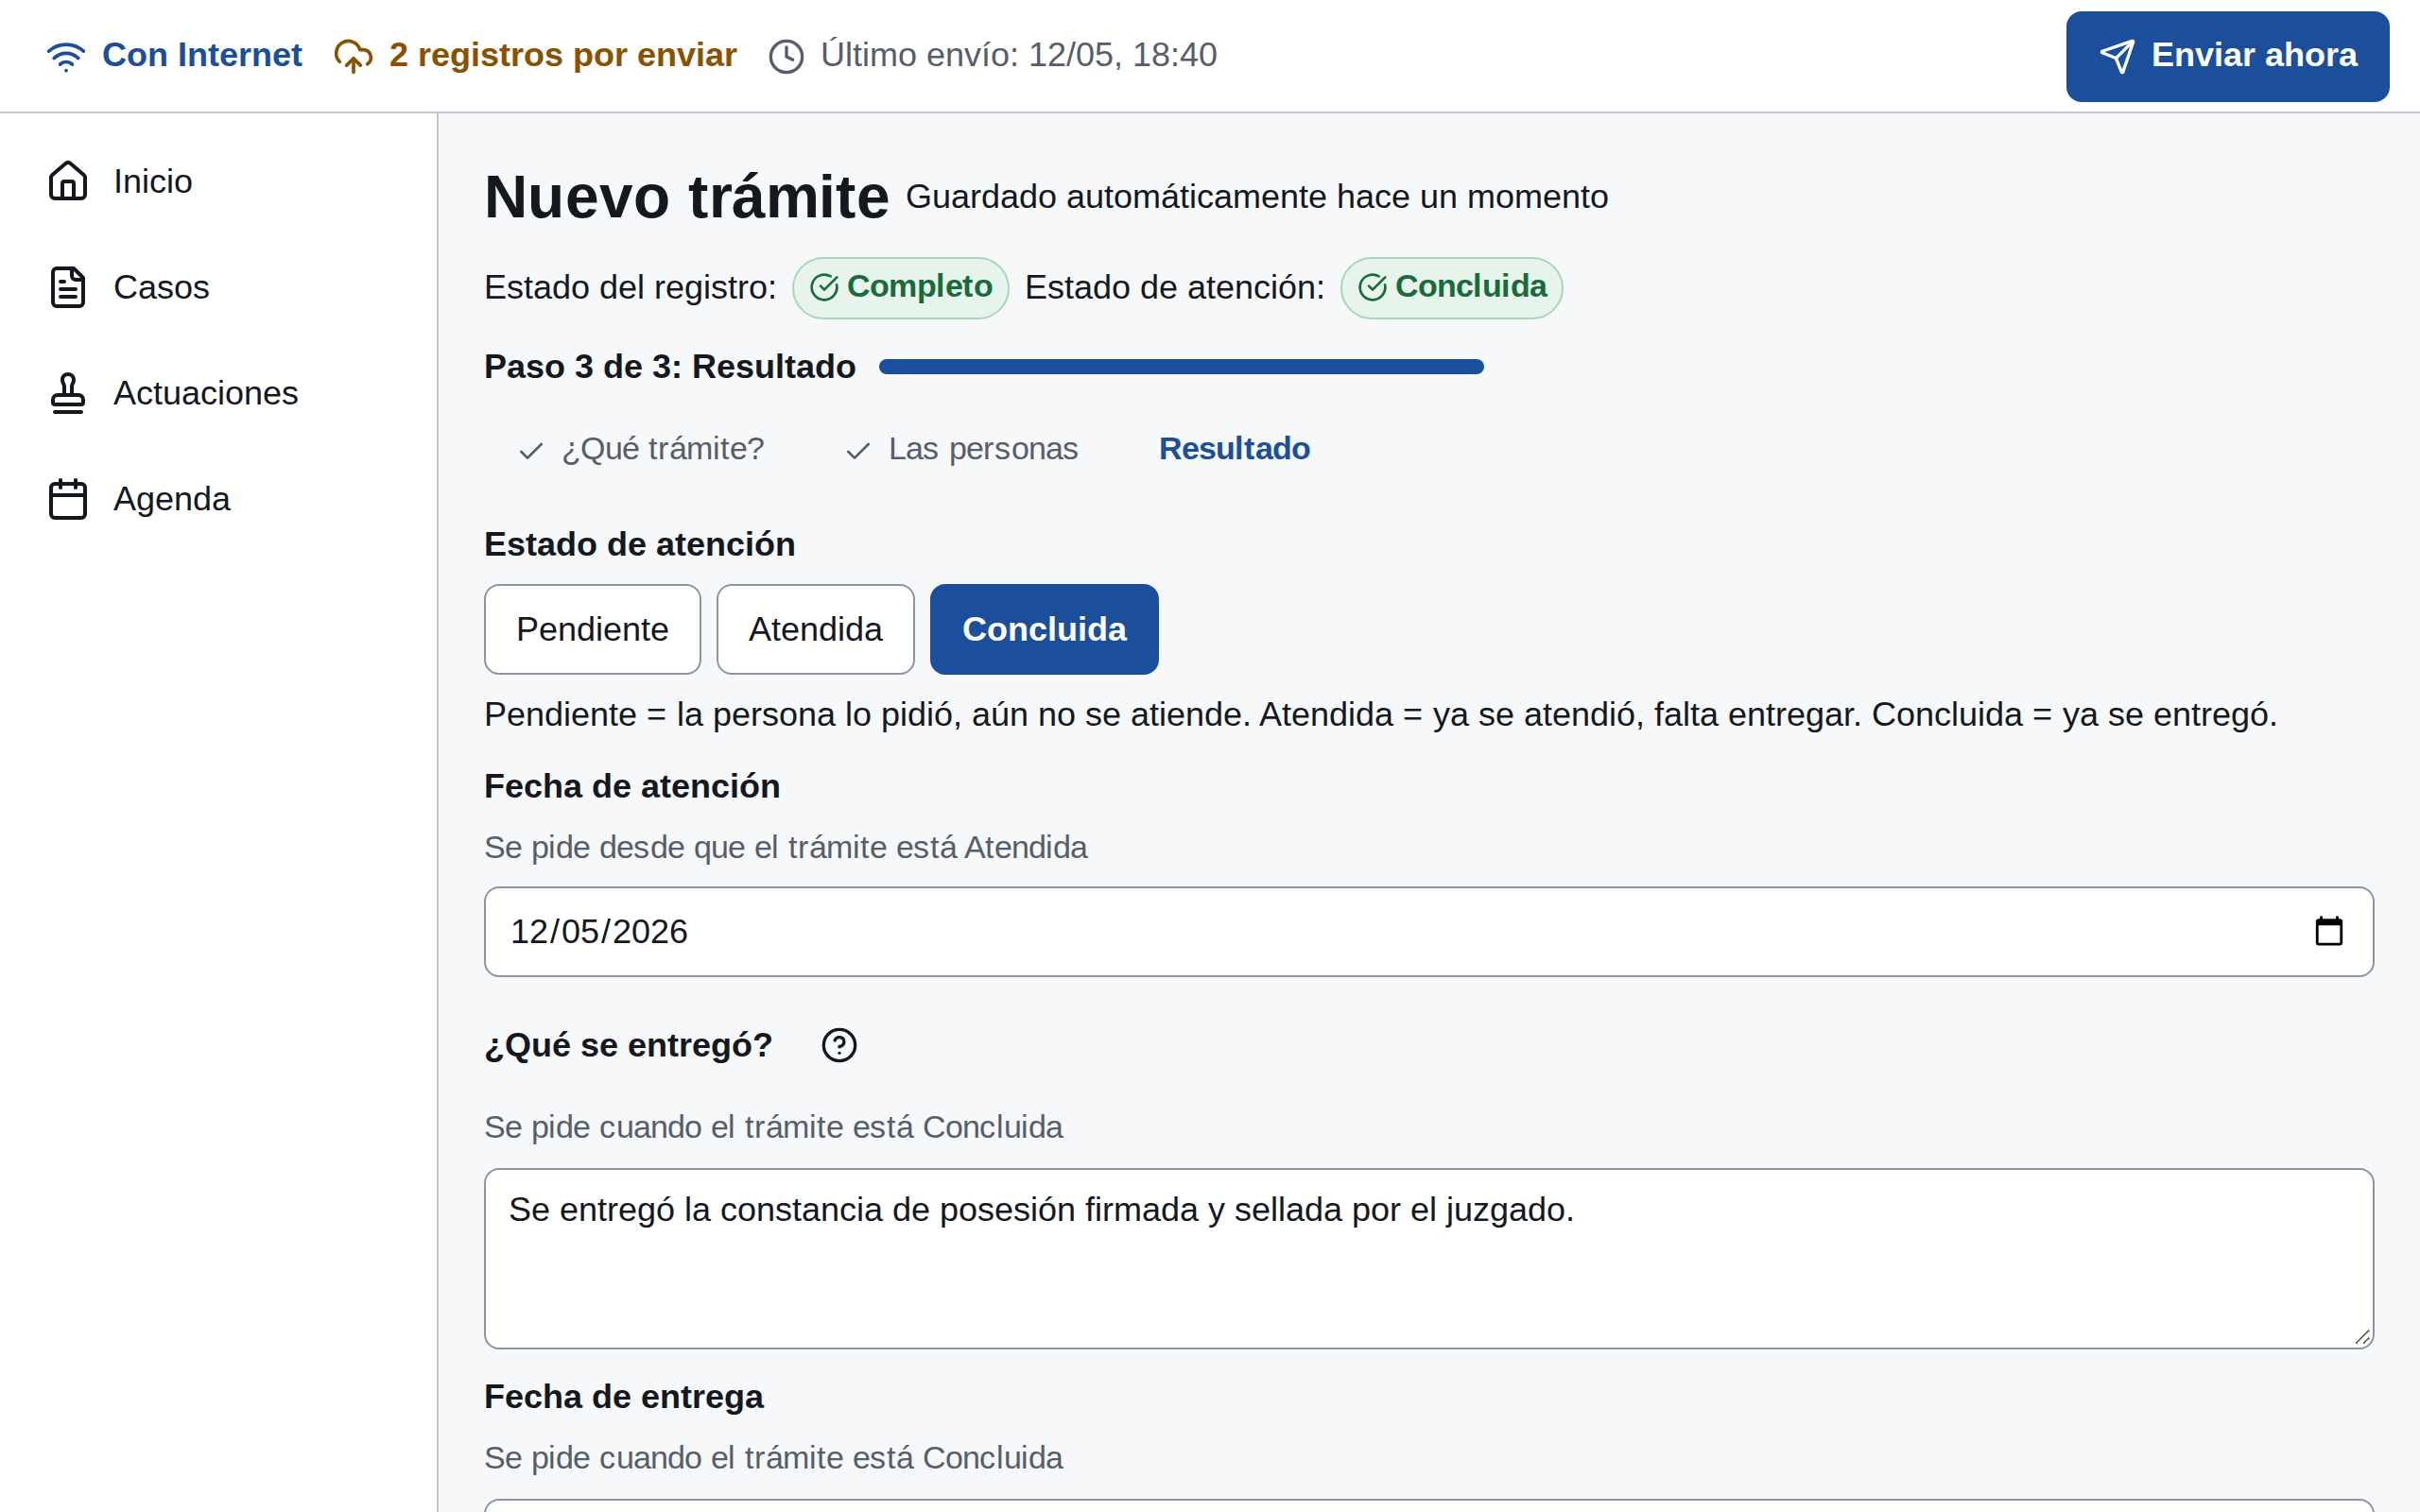
\includegraphics[width=0.82\linewidth]{capturas/F2-07_completo.png}
\caption{P-06 · 5. De Borrador a Completo. El estado del registro pasa a Completo, separado del estado de atención}
\end{figure}
\begin{figure}[H]\centering
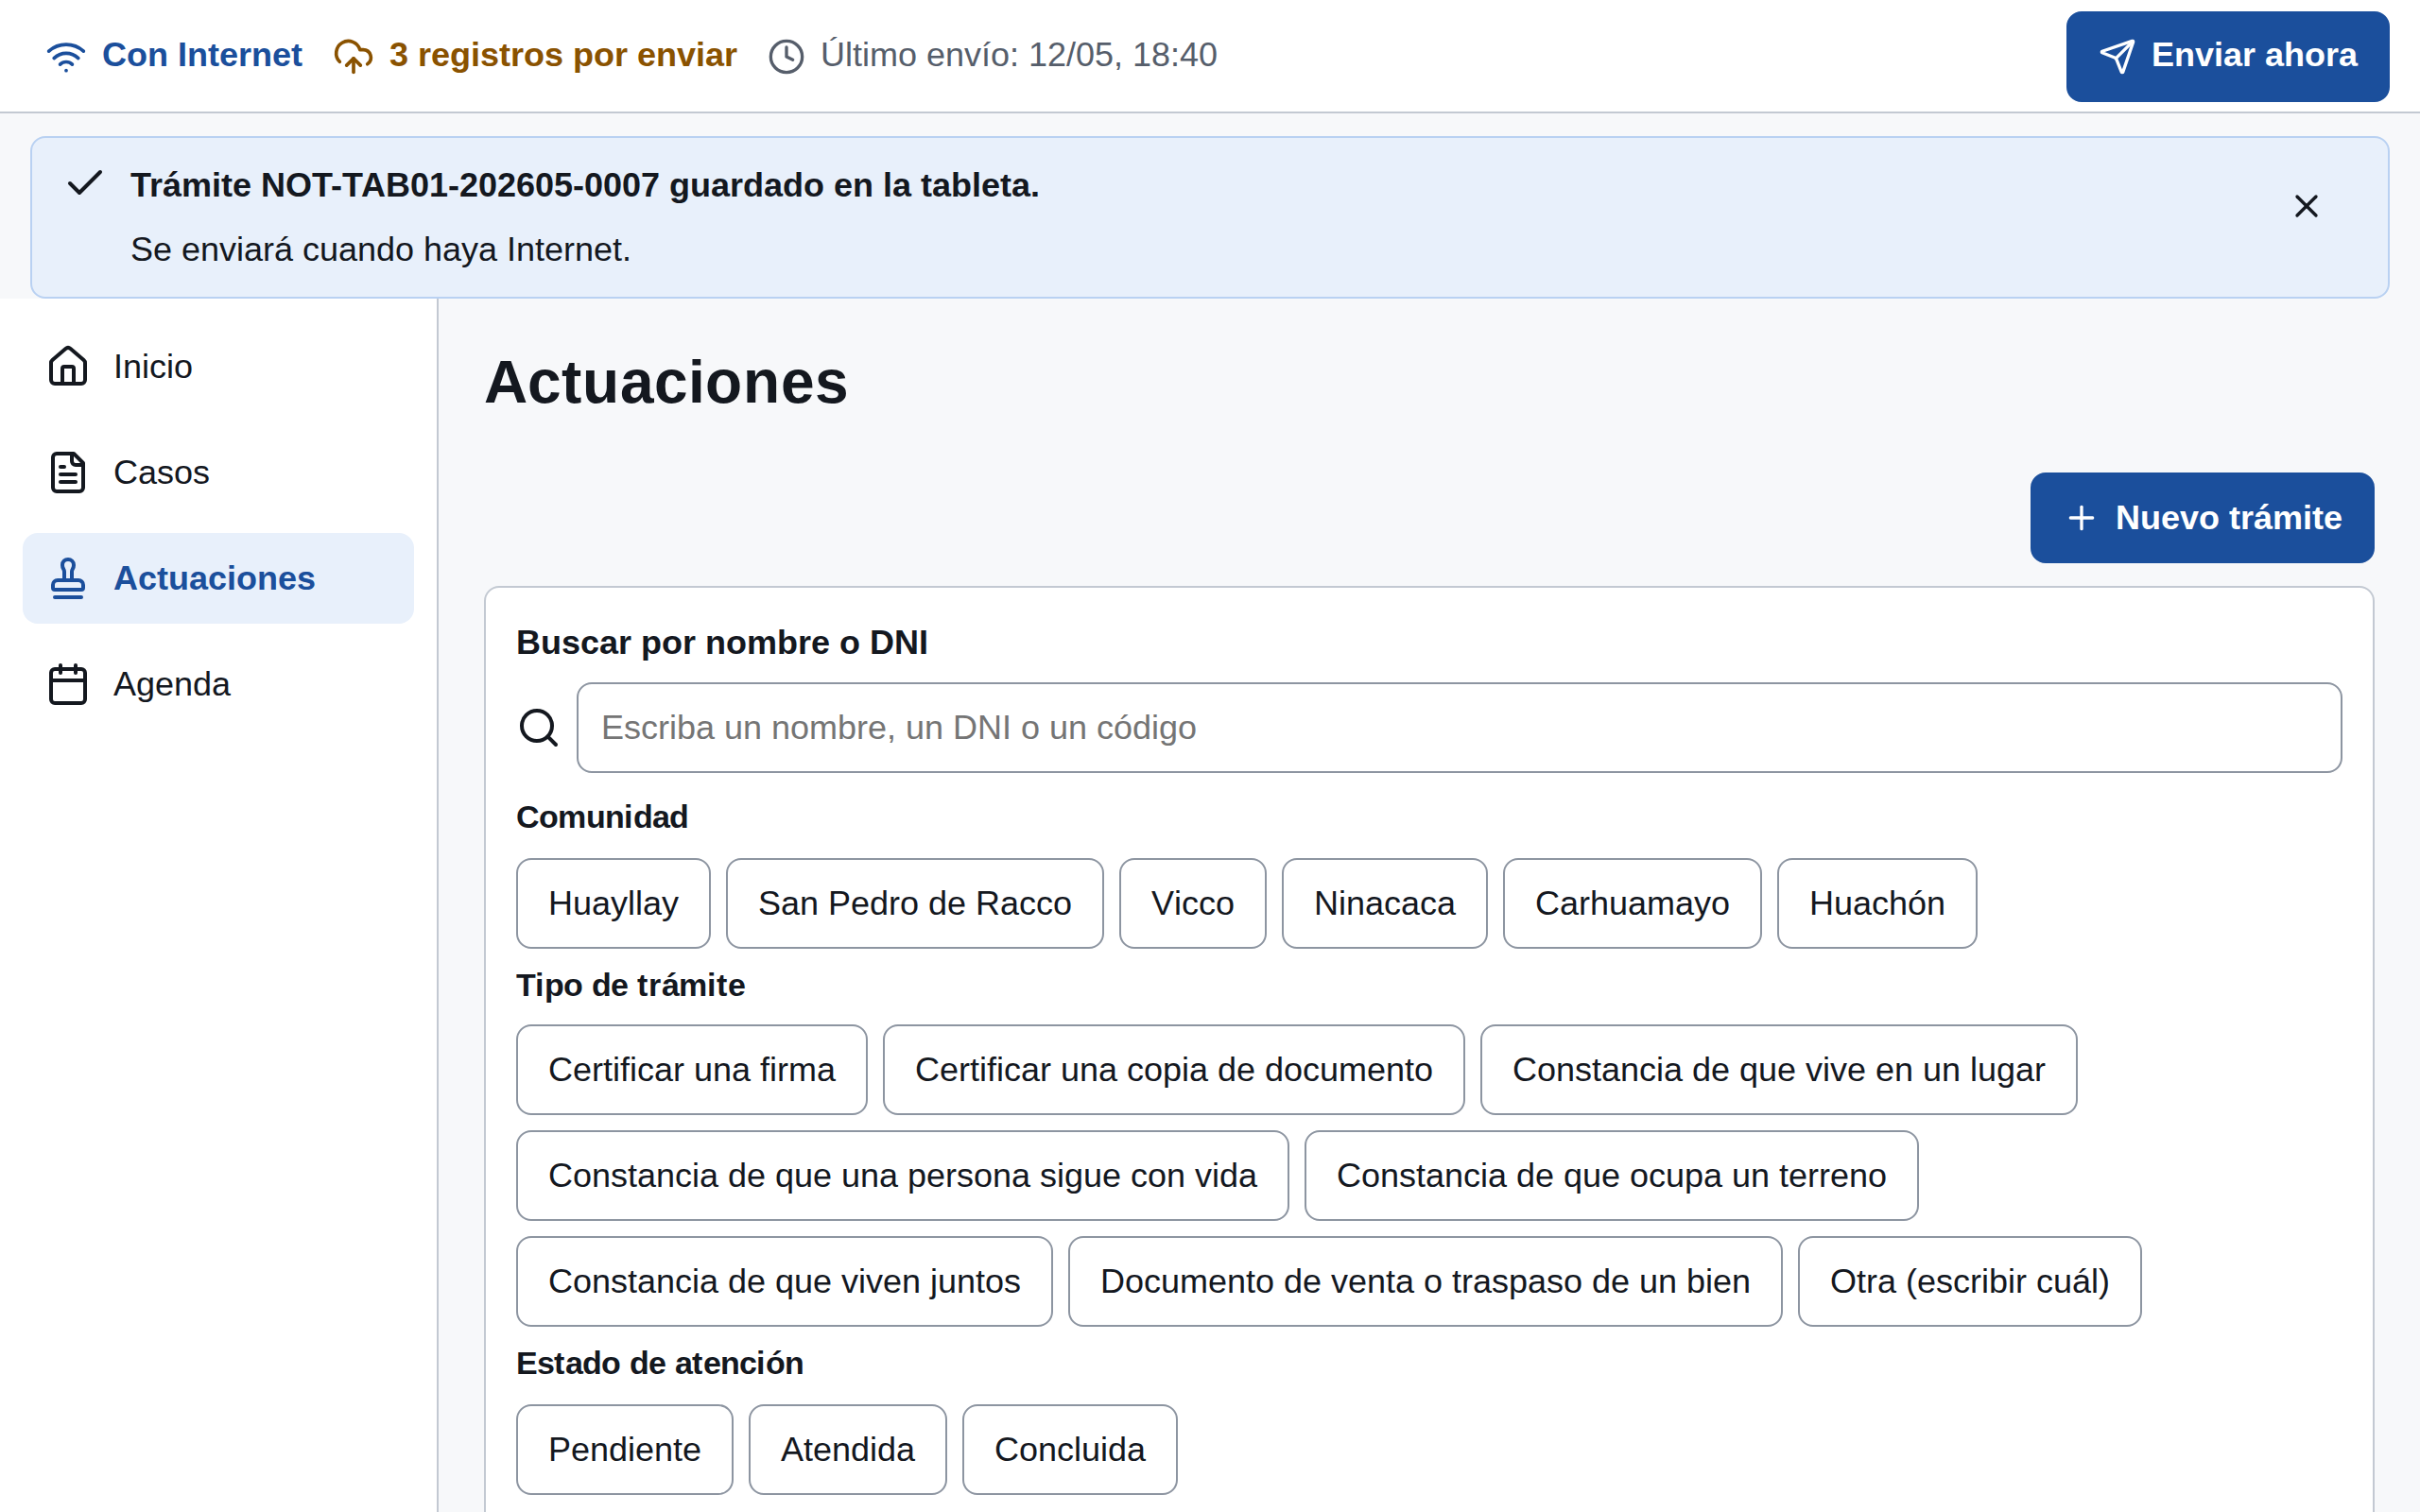
\includegraphics[width=0.82\linewidth]{capturas/F2-08_confirmacion.png}
\caption{P-05 · 6. Confirmación en la tableta. La confirmación dice dónde quedó el trámite y la barra sube su contador a 3}
\end{figure}
\subsection{Flujo 3 · Revisar las actividades de la semana}
\begin{figure}[H]\centering
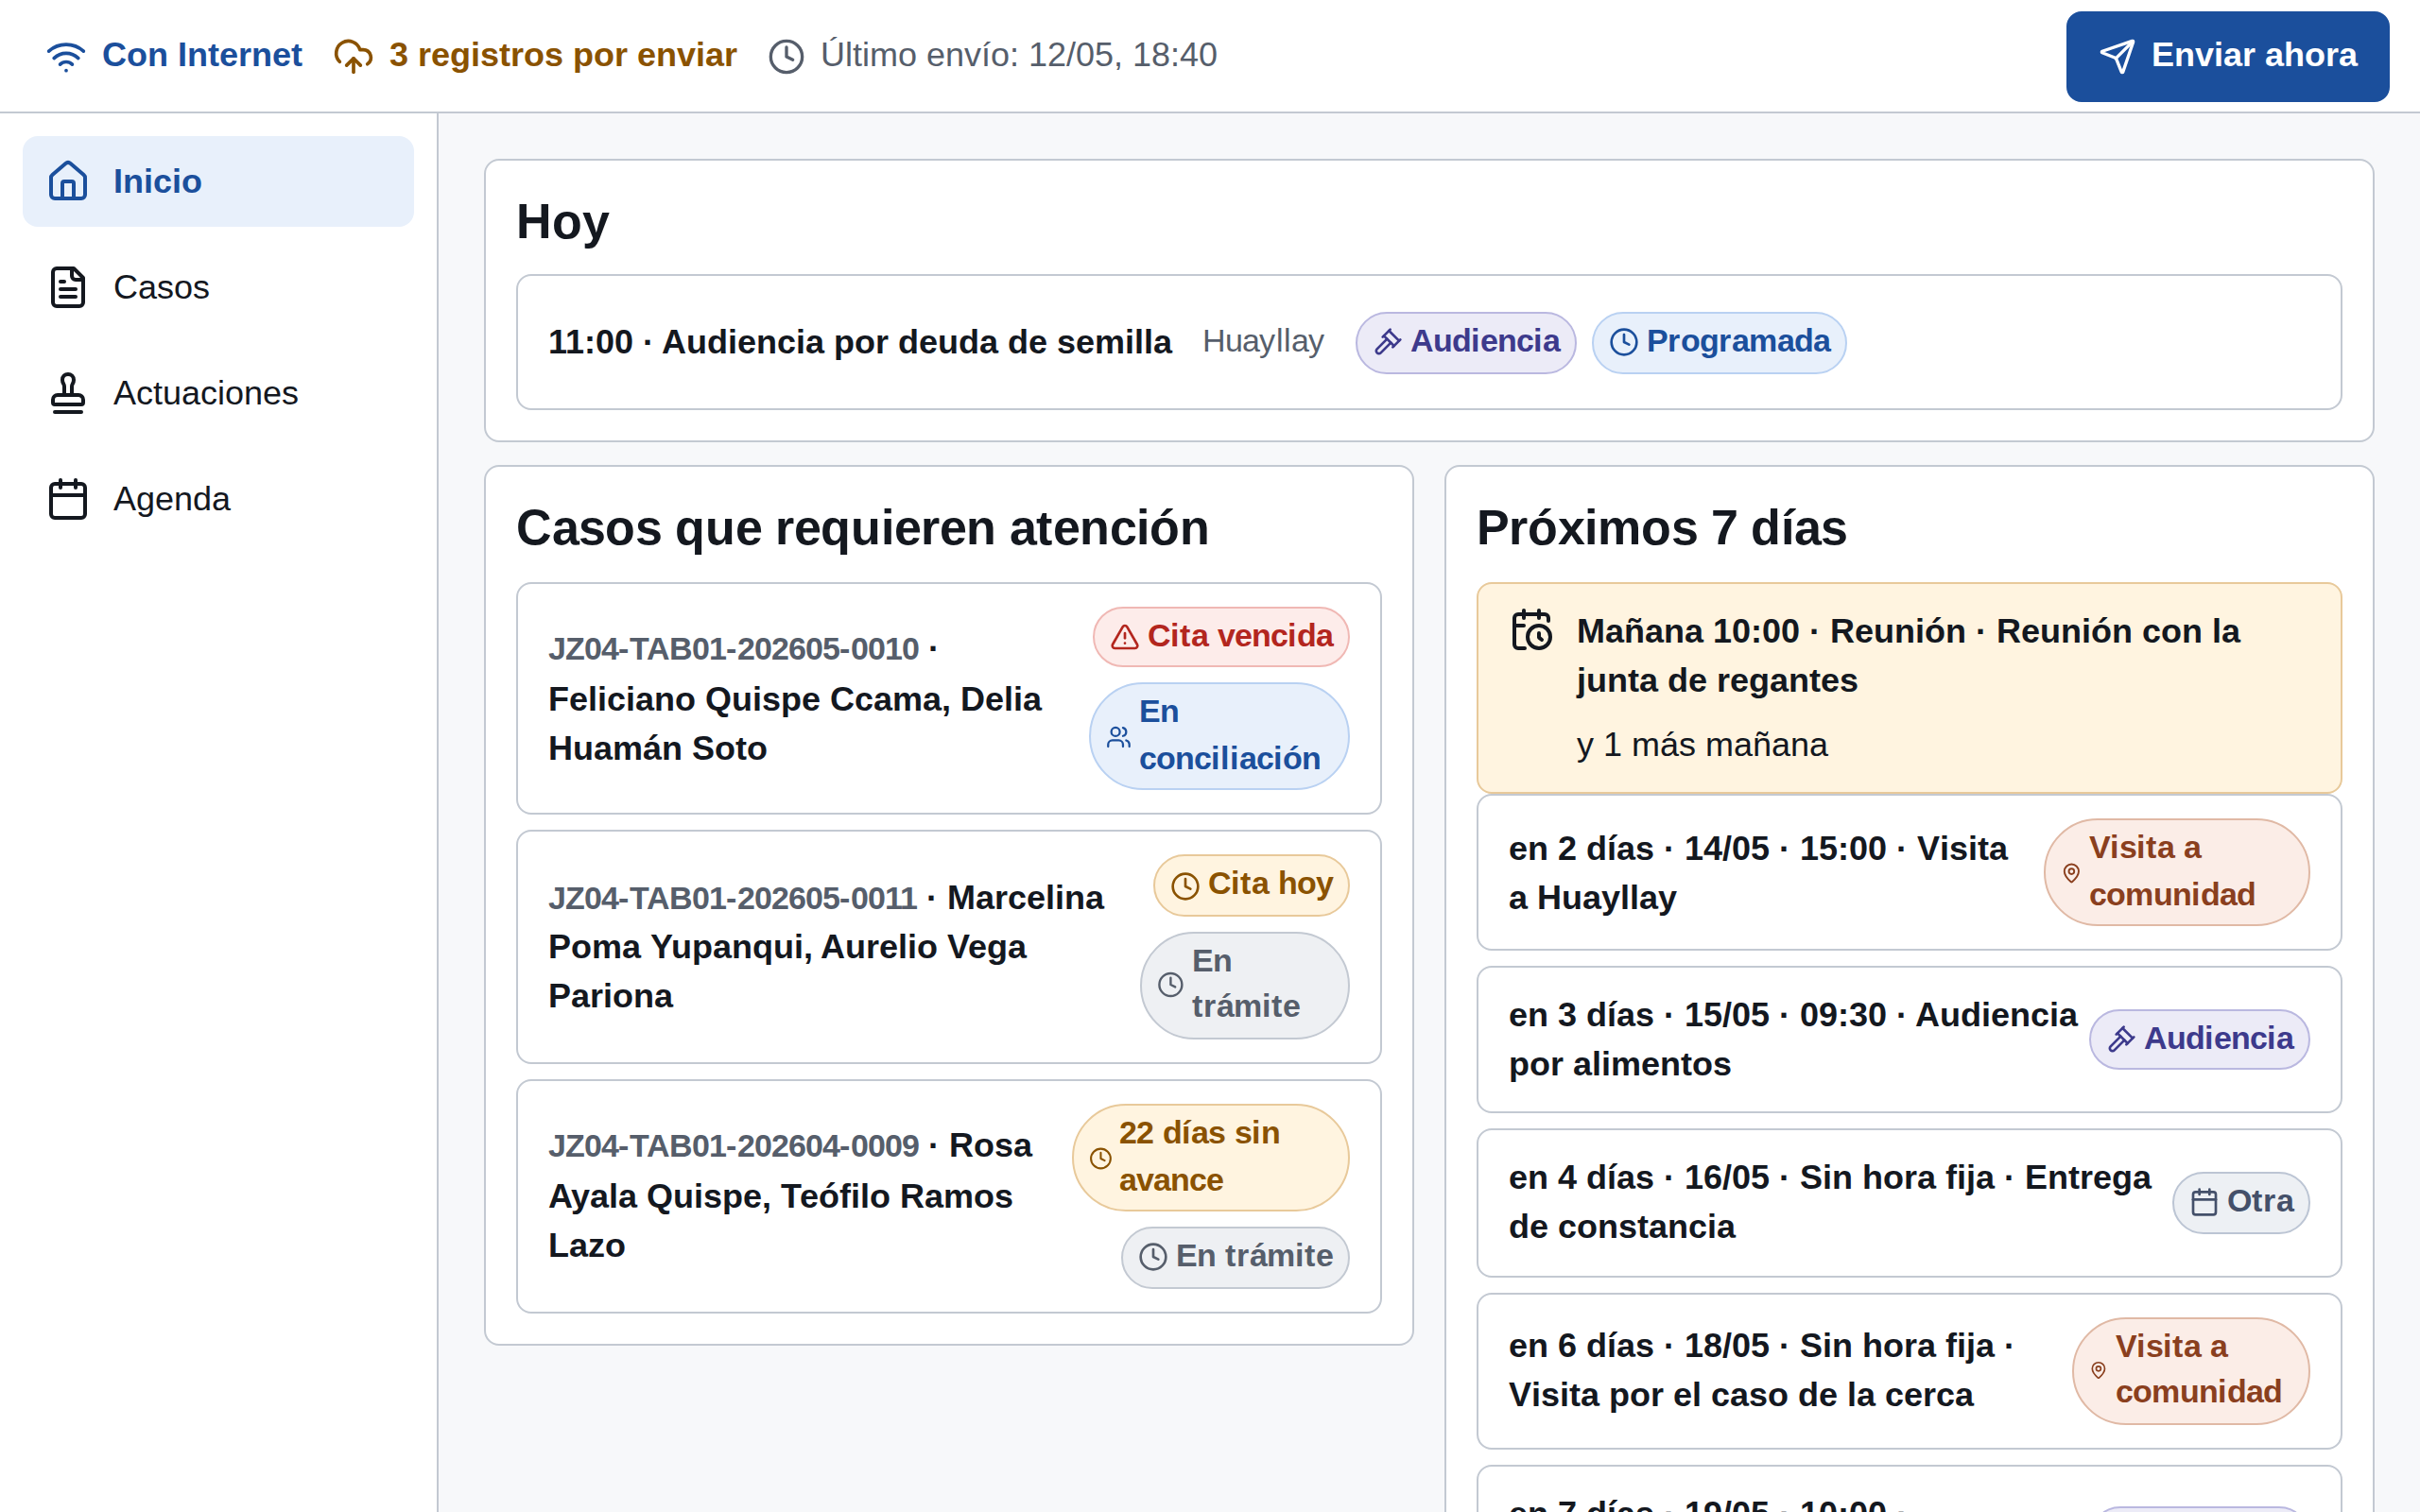
\includegraphics[width=0.82\linewidth]{capturas/F3-01_aviso-manana.png}
\caption{P-01 · 1. Aviso de lo de mañana. El aviso de mañana aparece sin que la jueza tenga que ir a buscarlo}
\end{figure}
\begin{figure}[H]\centering
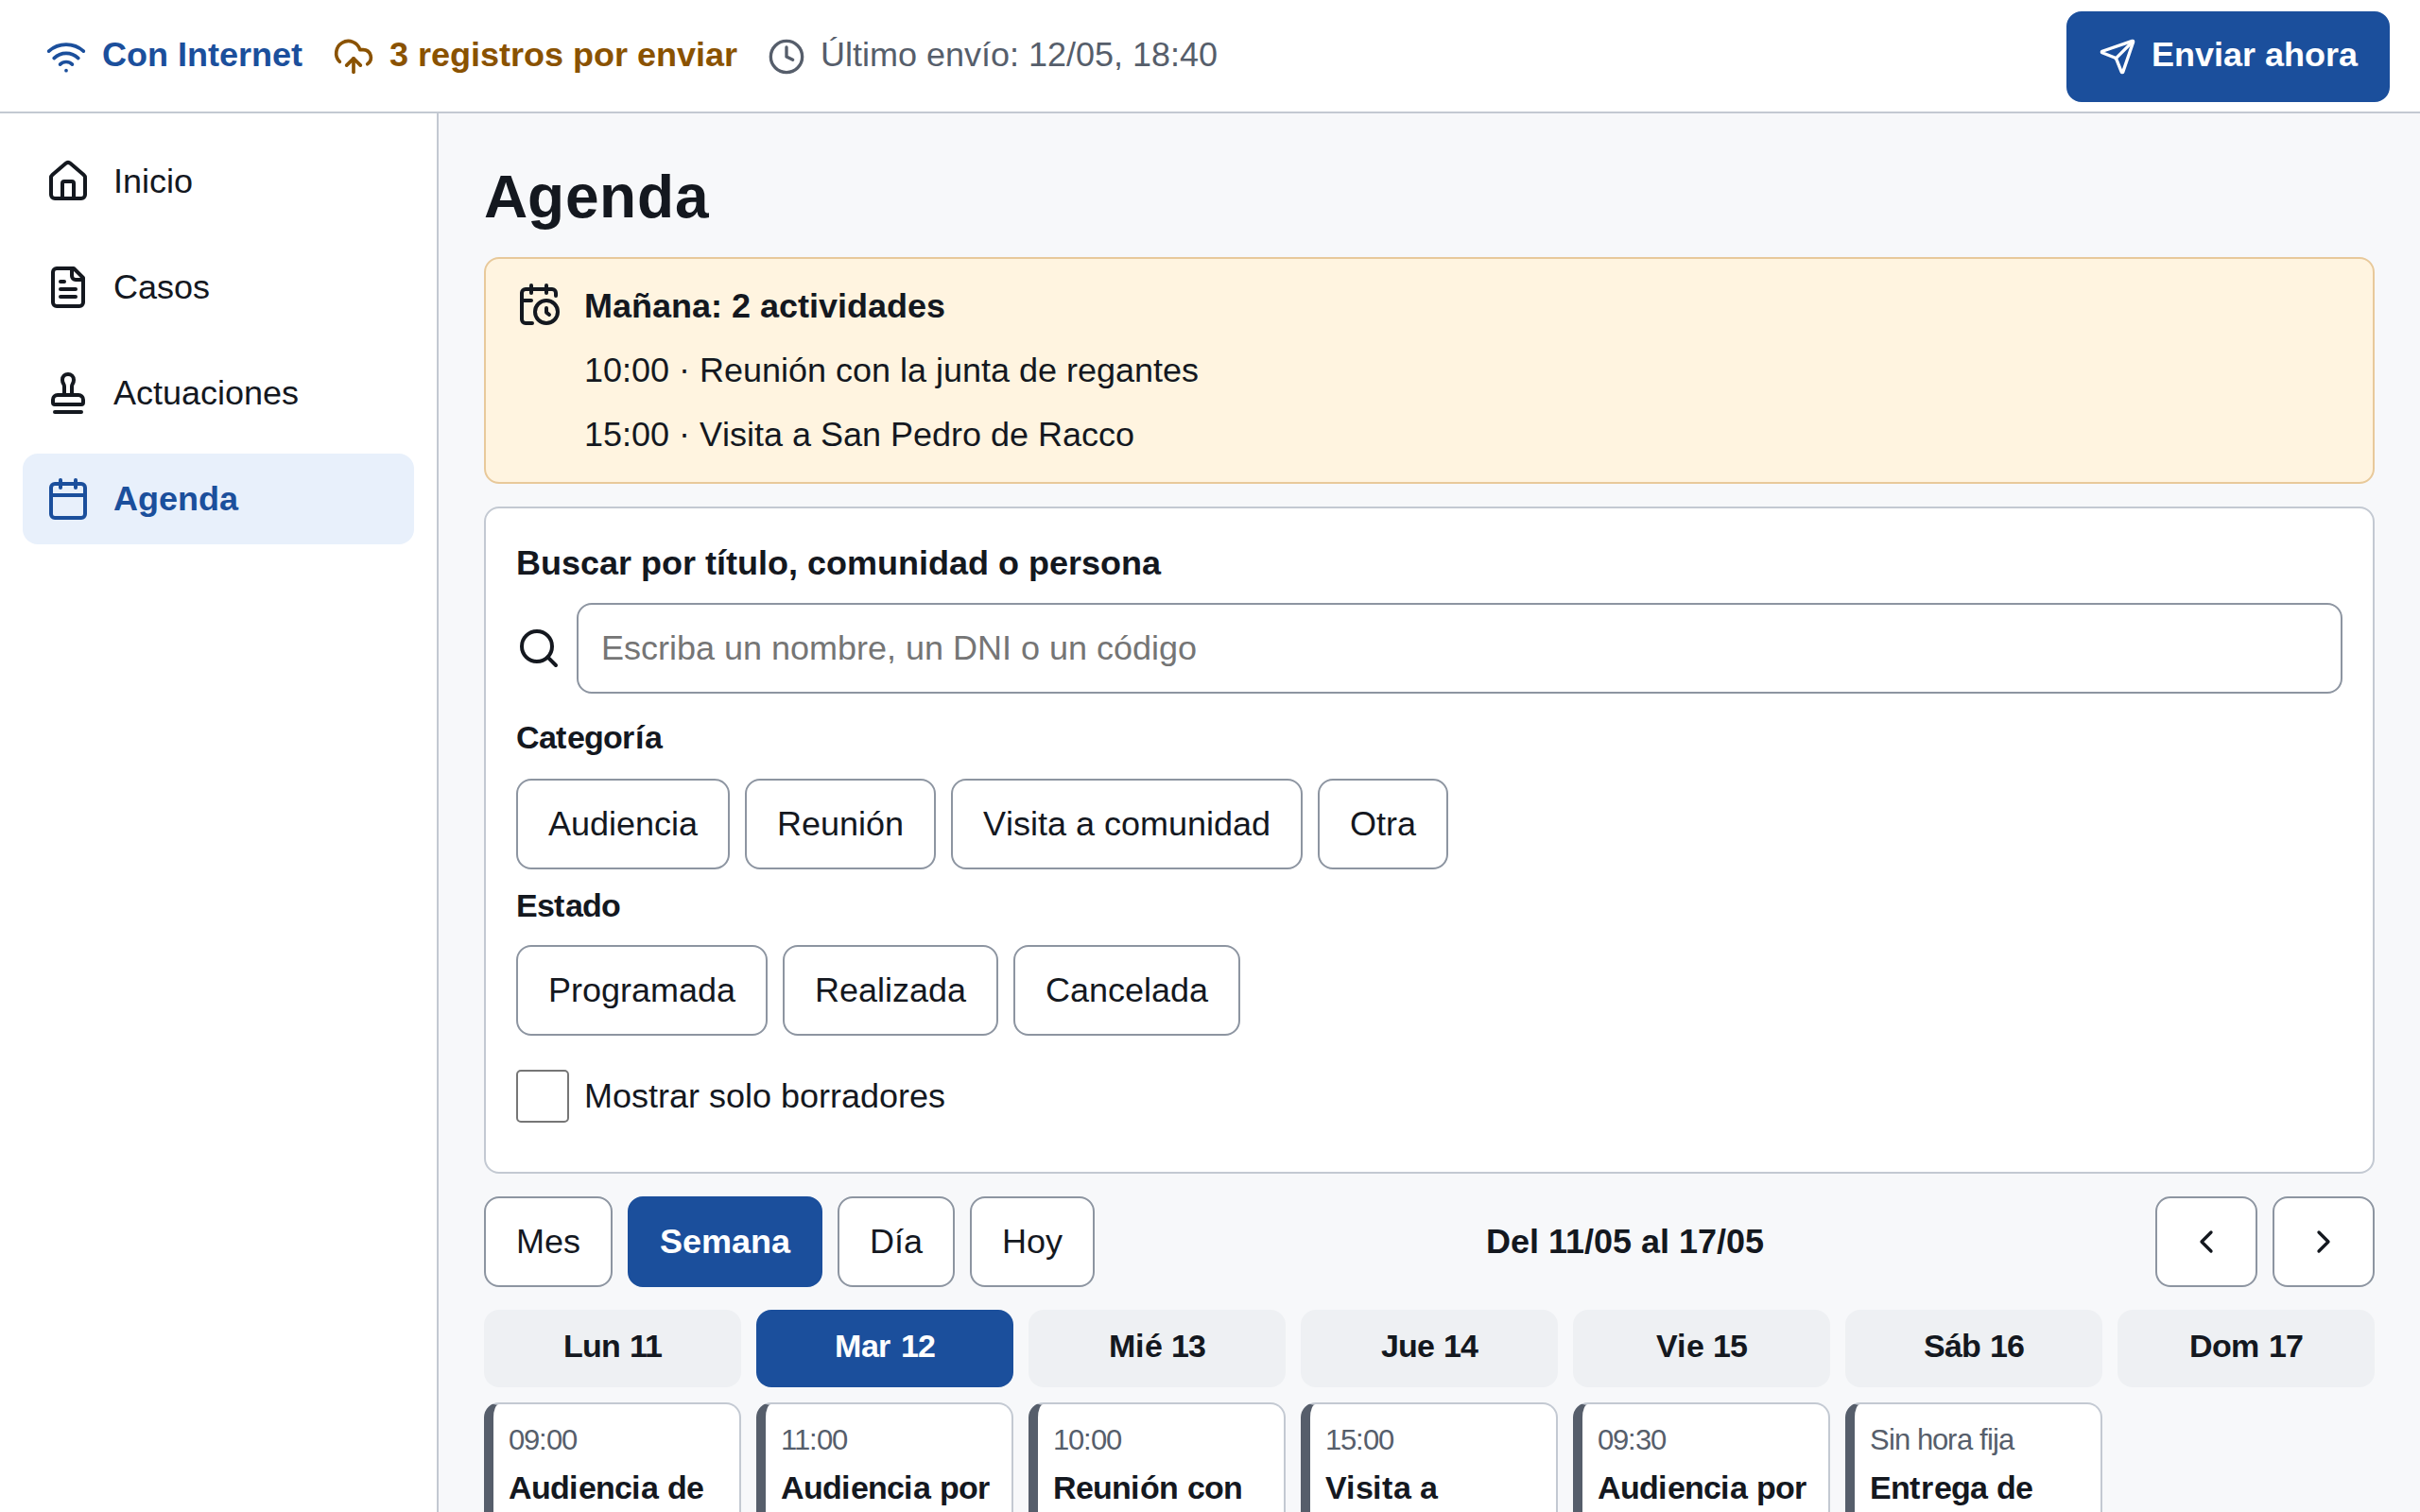
\includegraphics[width=0.82\linewidth]{capturas/F3-02_agenda-semana.png}
\caption{P-07 · 2. Vista semana. Categorías con color, ícono y texto; estados de cada actividad}
\end{figure}
\begin{figure}[H]\centering
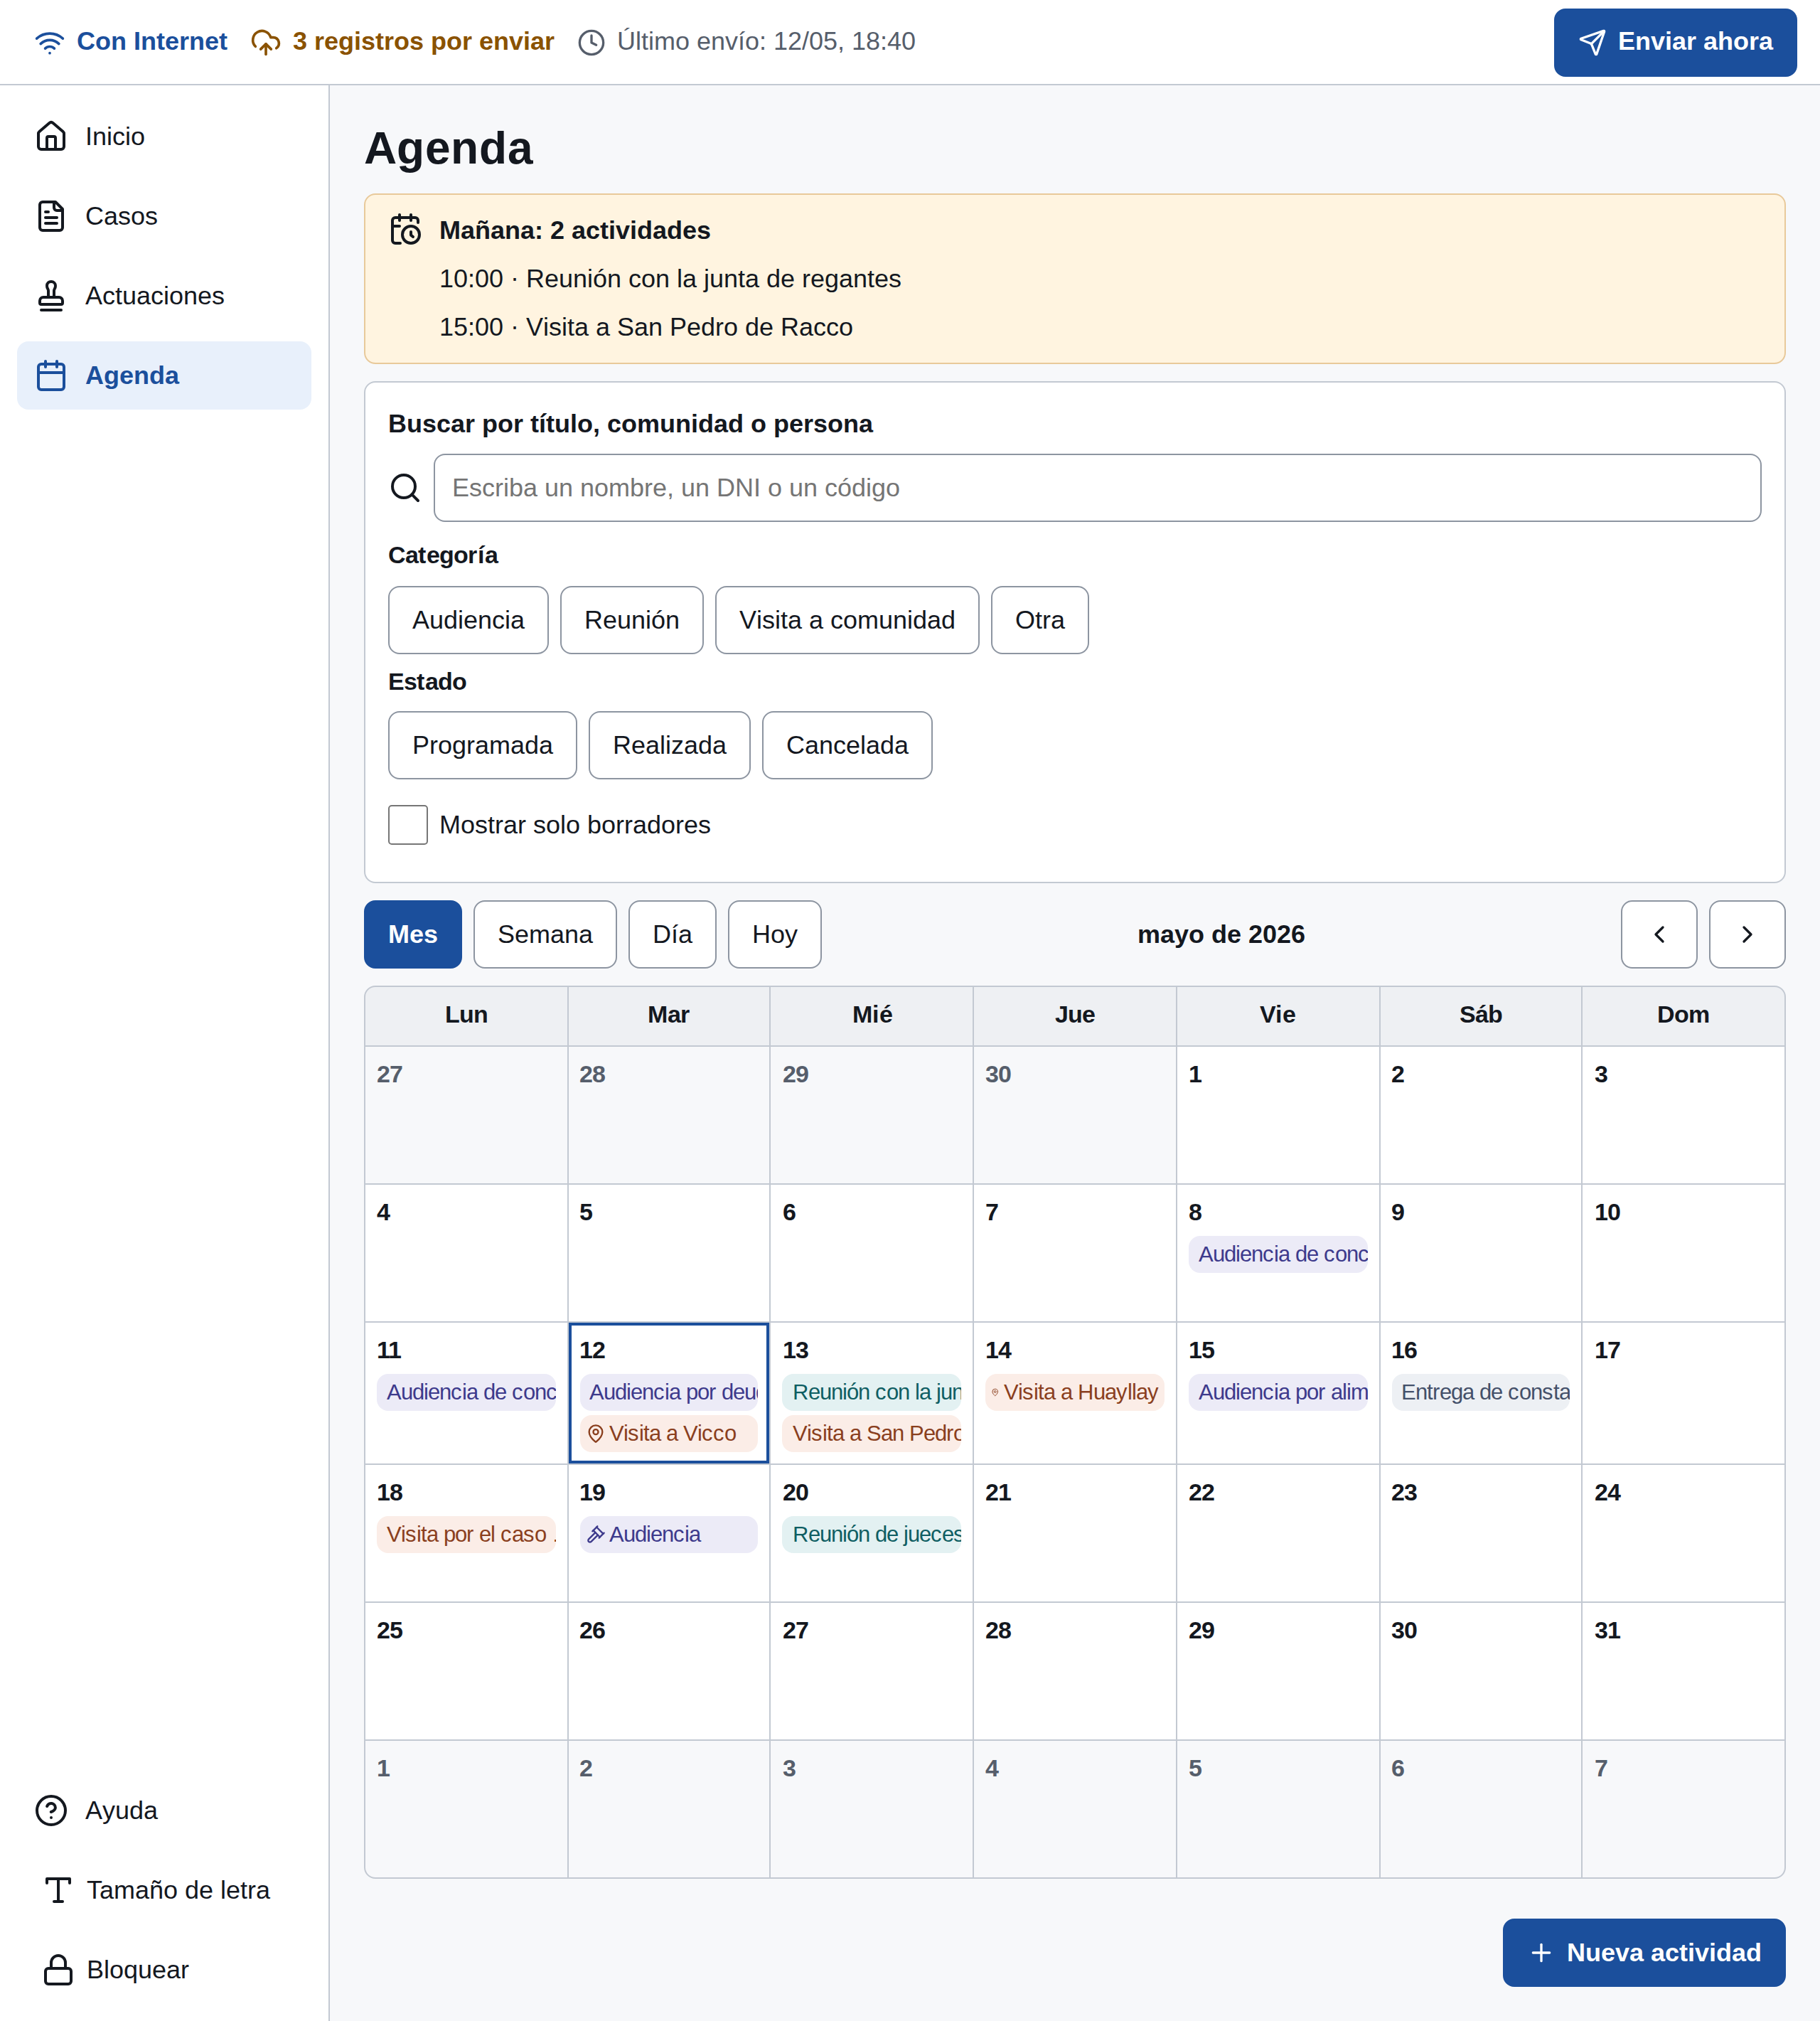
\includegraphics[width=0.82\linewidth]{capturas/F3-03_agenda-mes.png}
\caption{P-07 · 2. Vista mes. Vista mes con las actividades de cada día en píldoras de color y texto}
\end{figure}
\begin{figure}[H]\centering
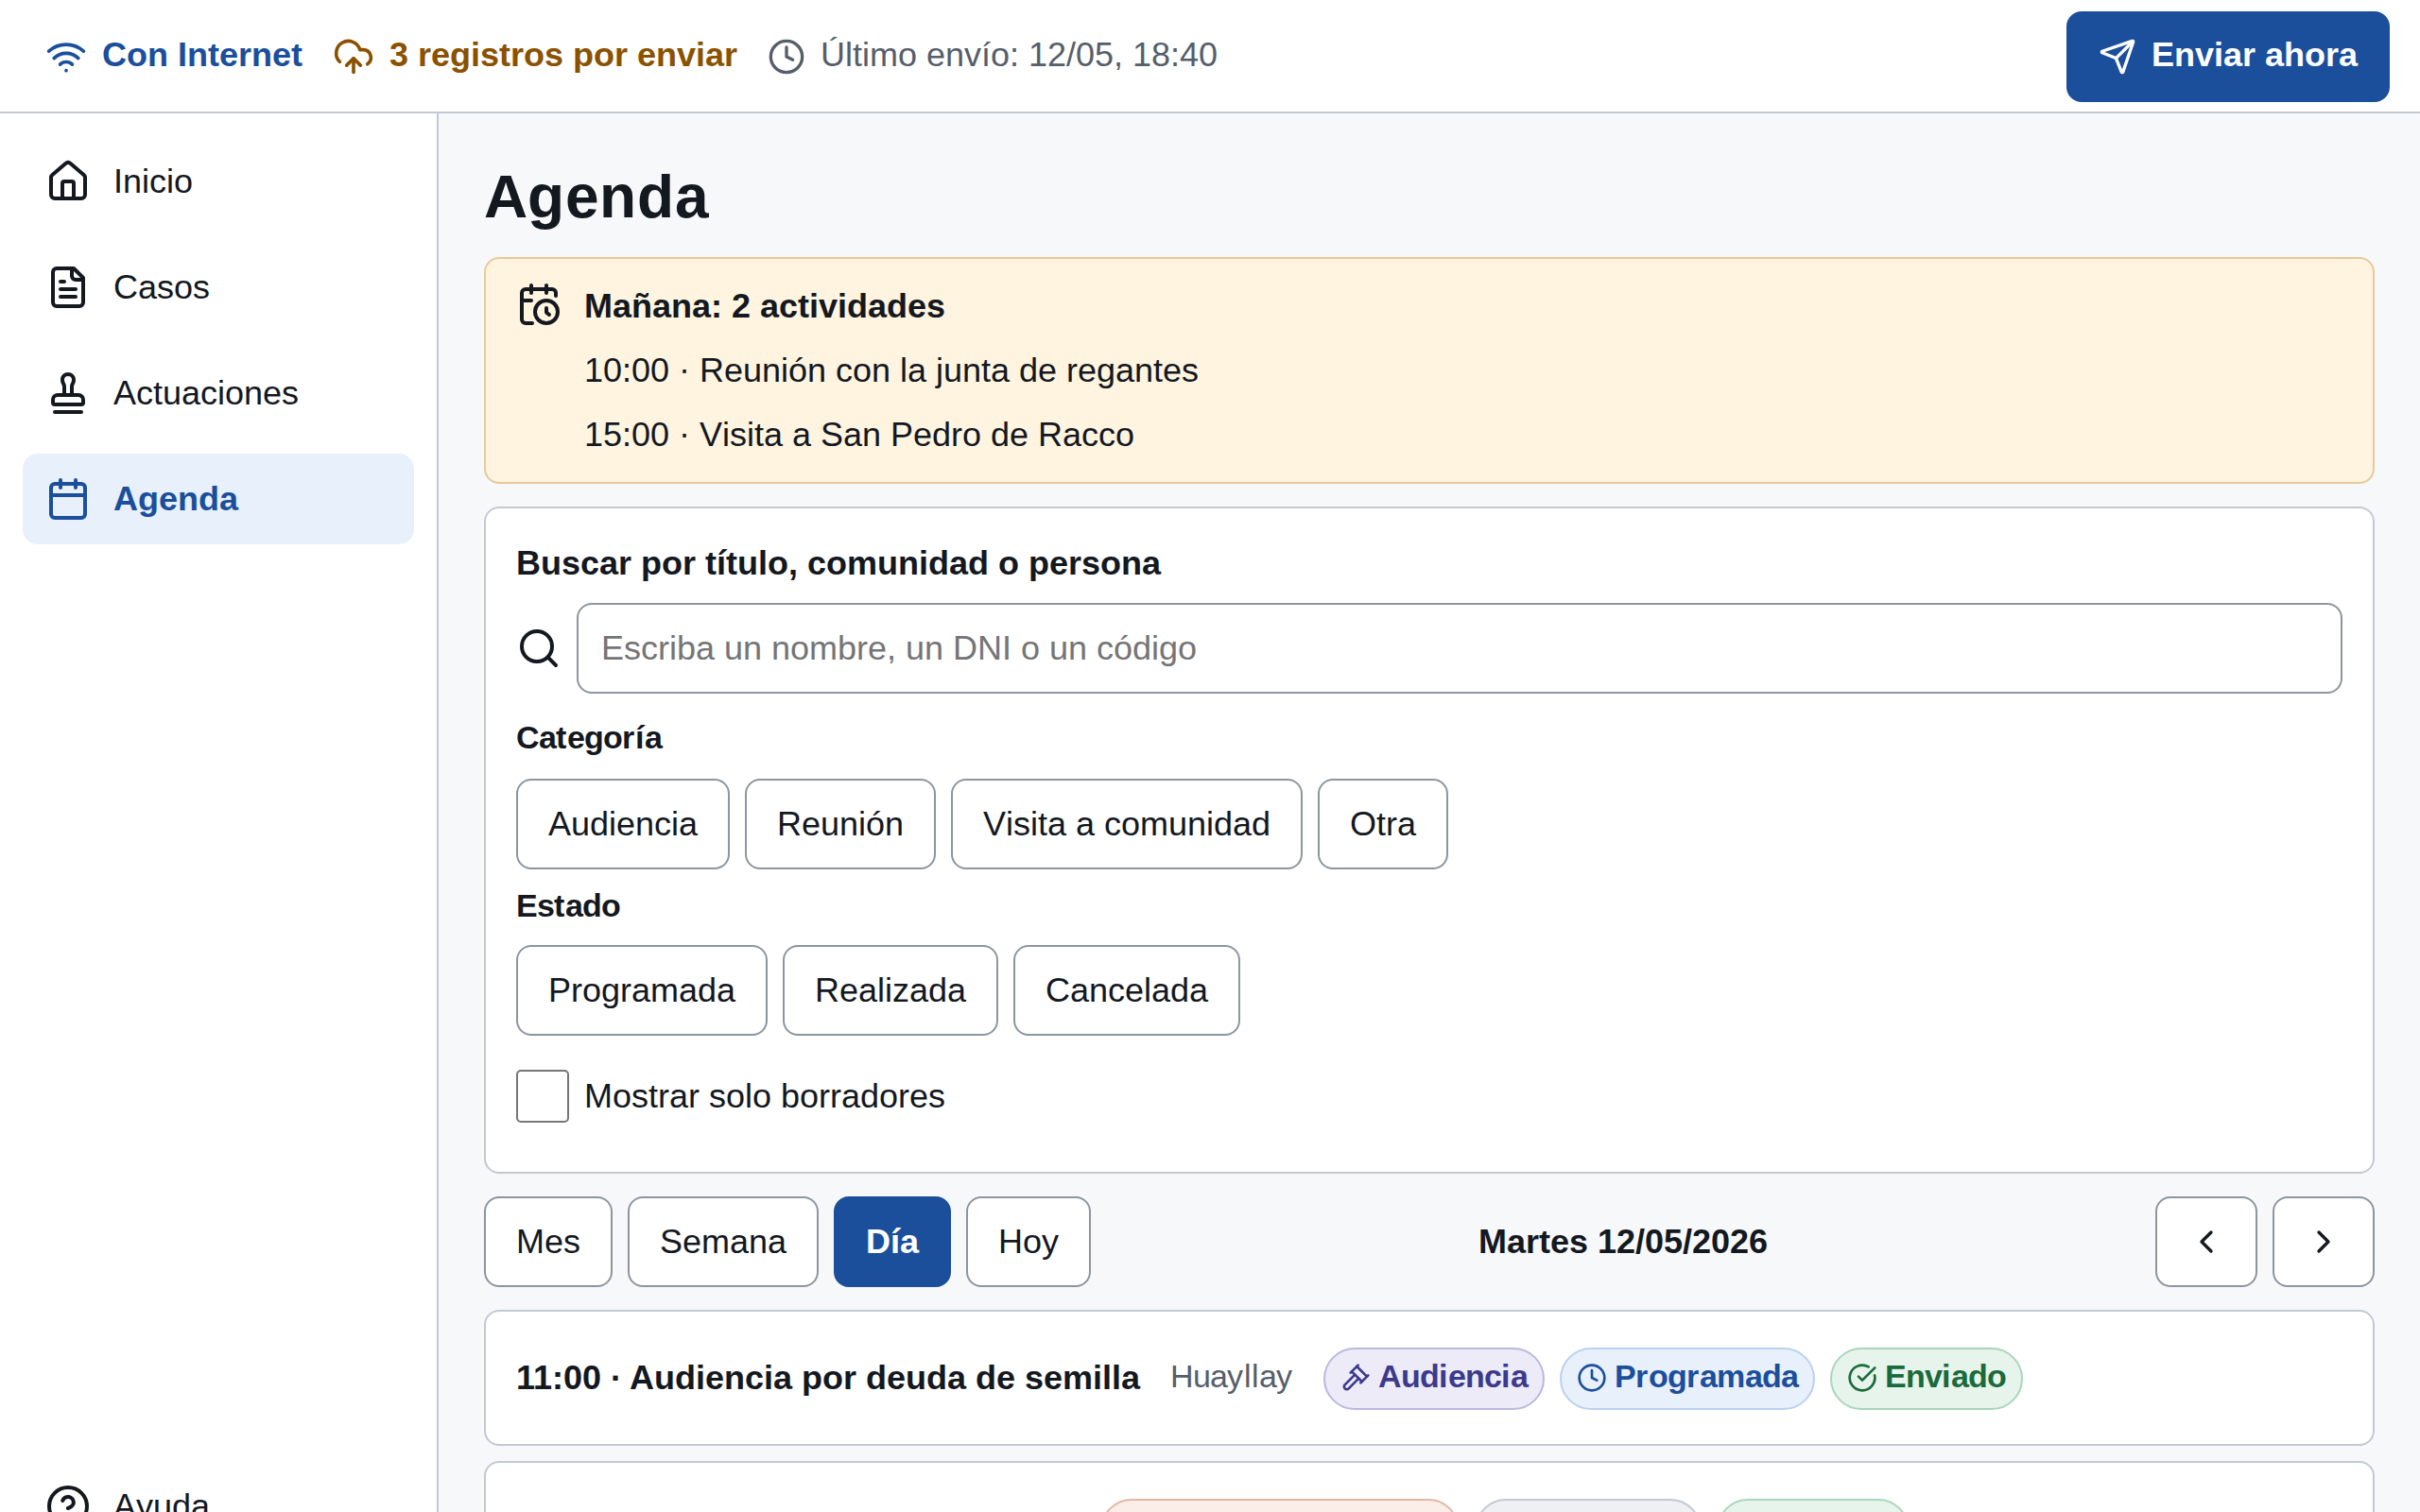
\includegraphics[width=0.82\linewidth]{capturas/F3-04_agenda-dia.png}
\caption{P-07 · 3. Vista día. Vista día con el detalle de cada actividad}
\end{figure}
\begin{figure}[H]\centering
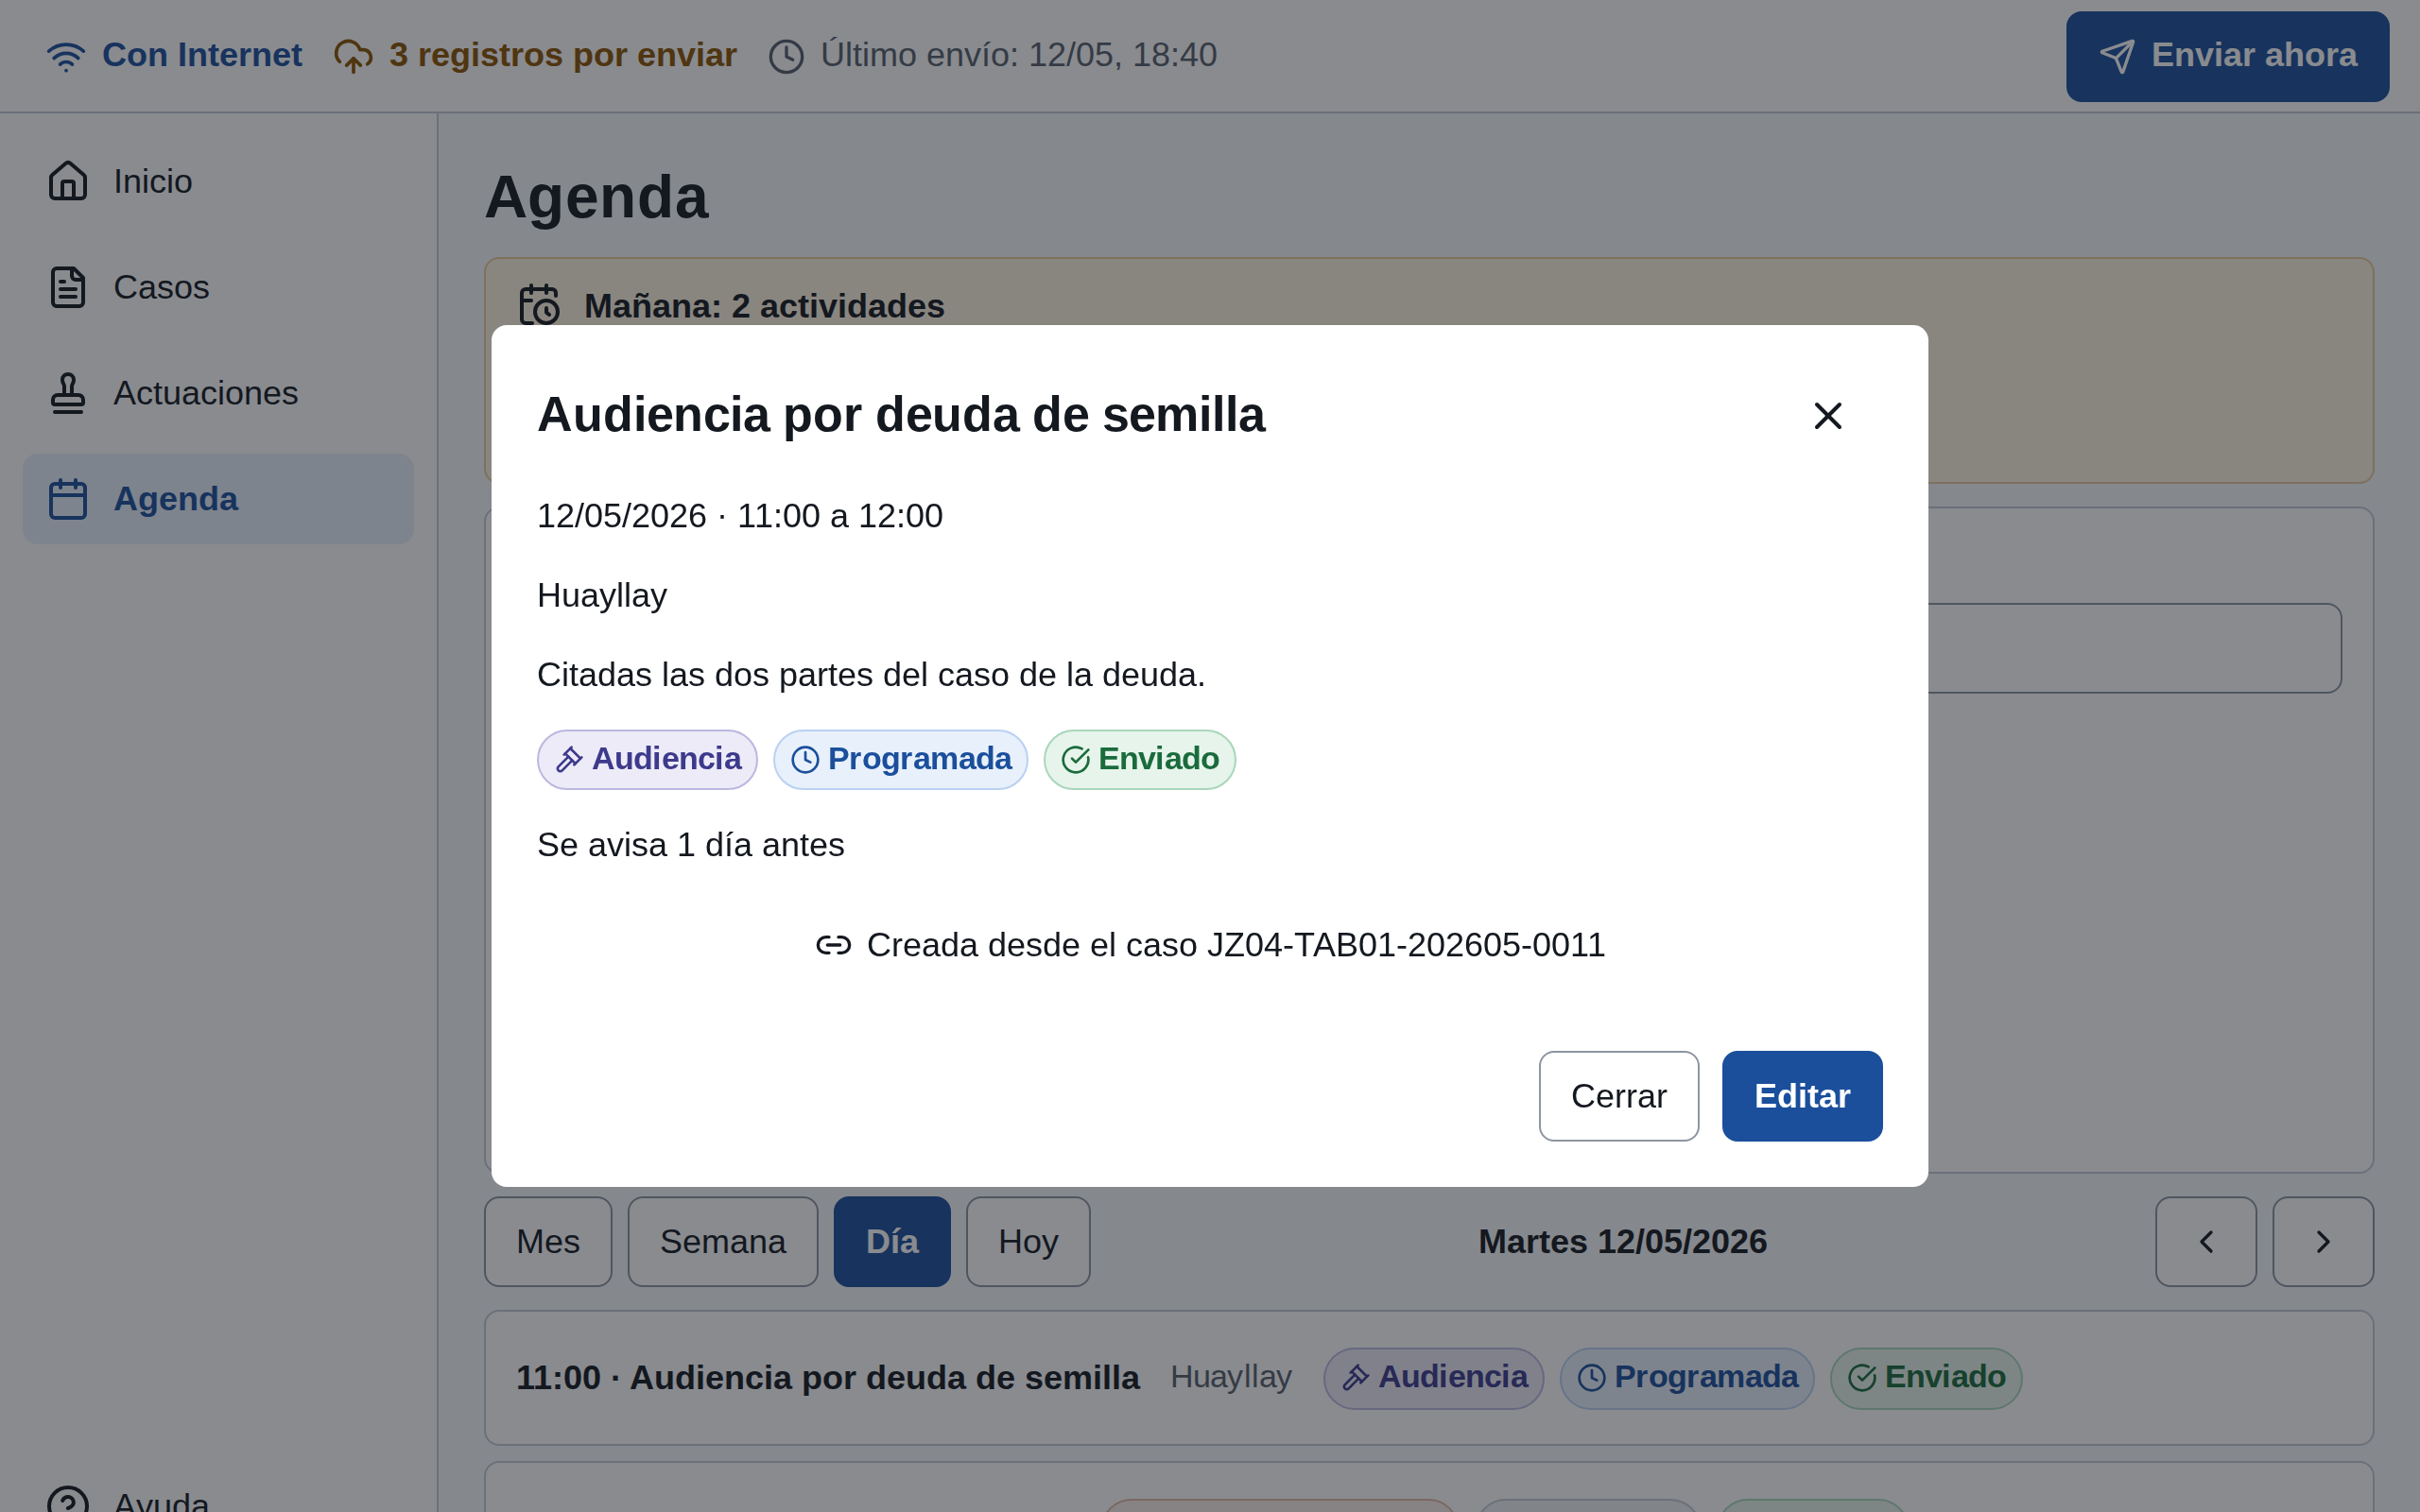
\includegraphics[width=0.82\linewidth]{capturas/F3-05_actividad-detalle.png}
\caption{P-07 · 3. Detalle con su vínculo al caso. La actividad muestra desde qué caso se creó y lleva a él}
\end{figure}
\subsection{Flujo 4 · Agendar una reunión y enviar todo}
\begin{figure}[H]\centering
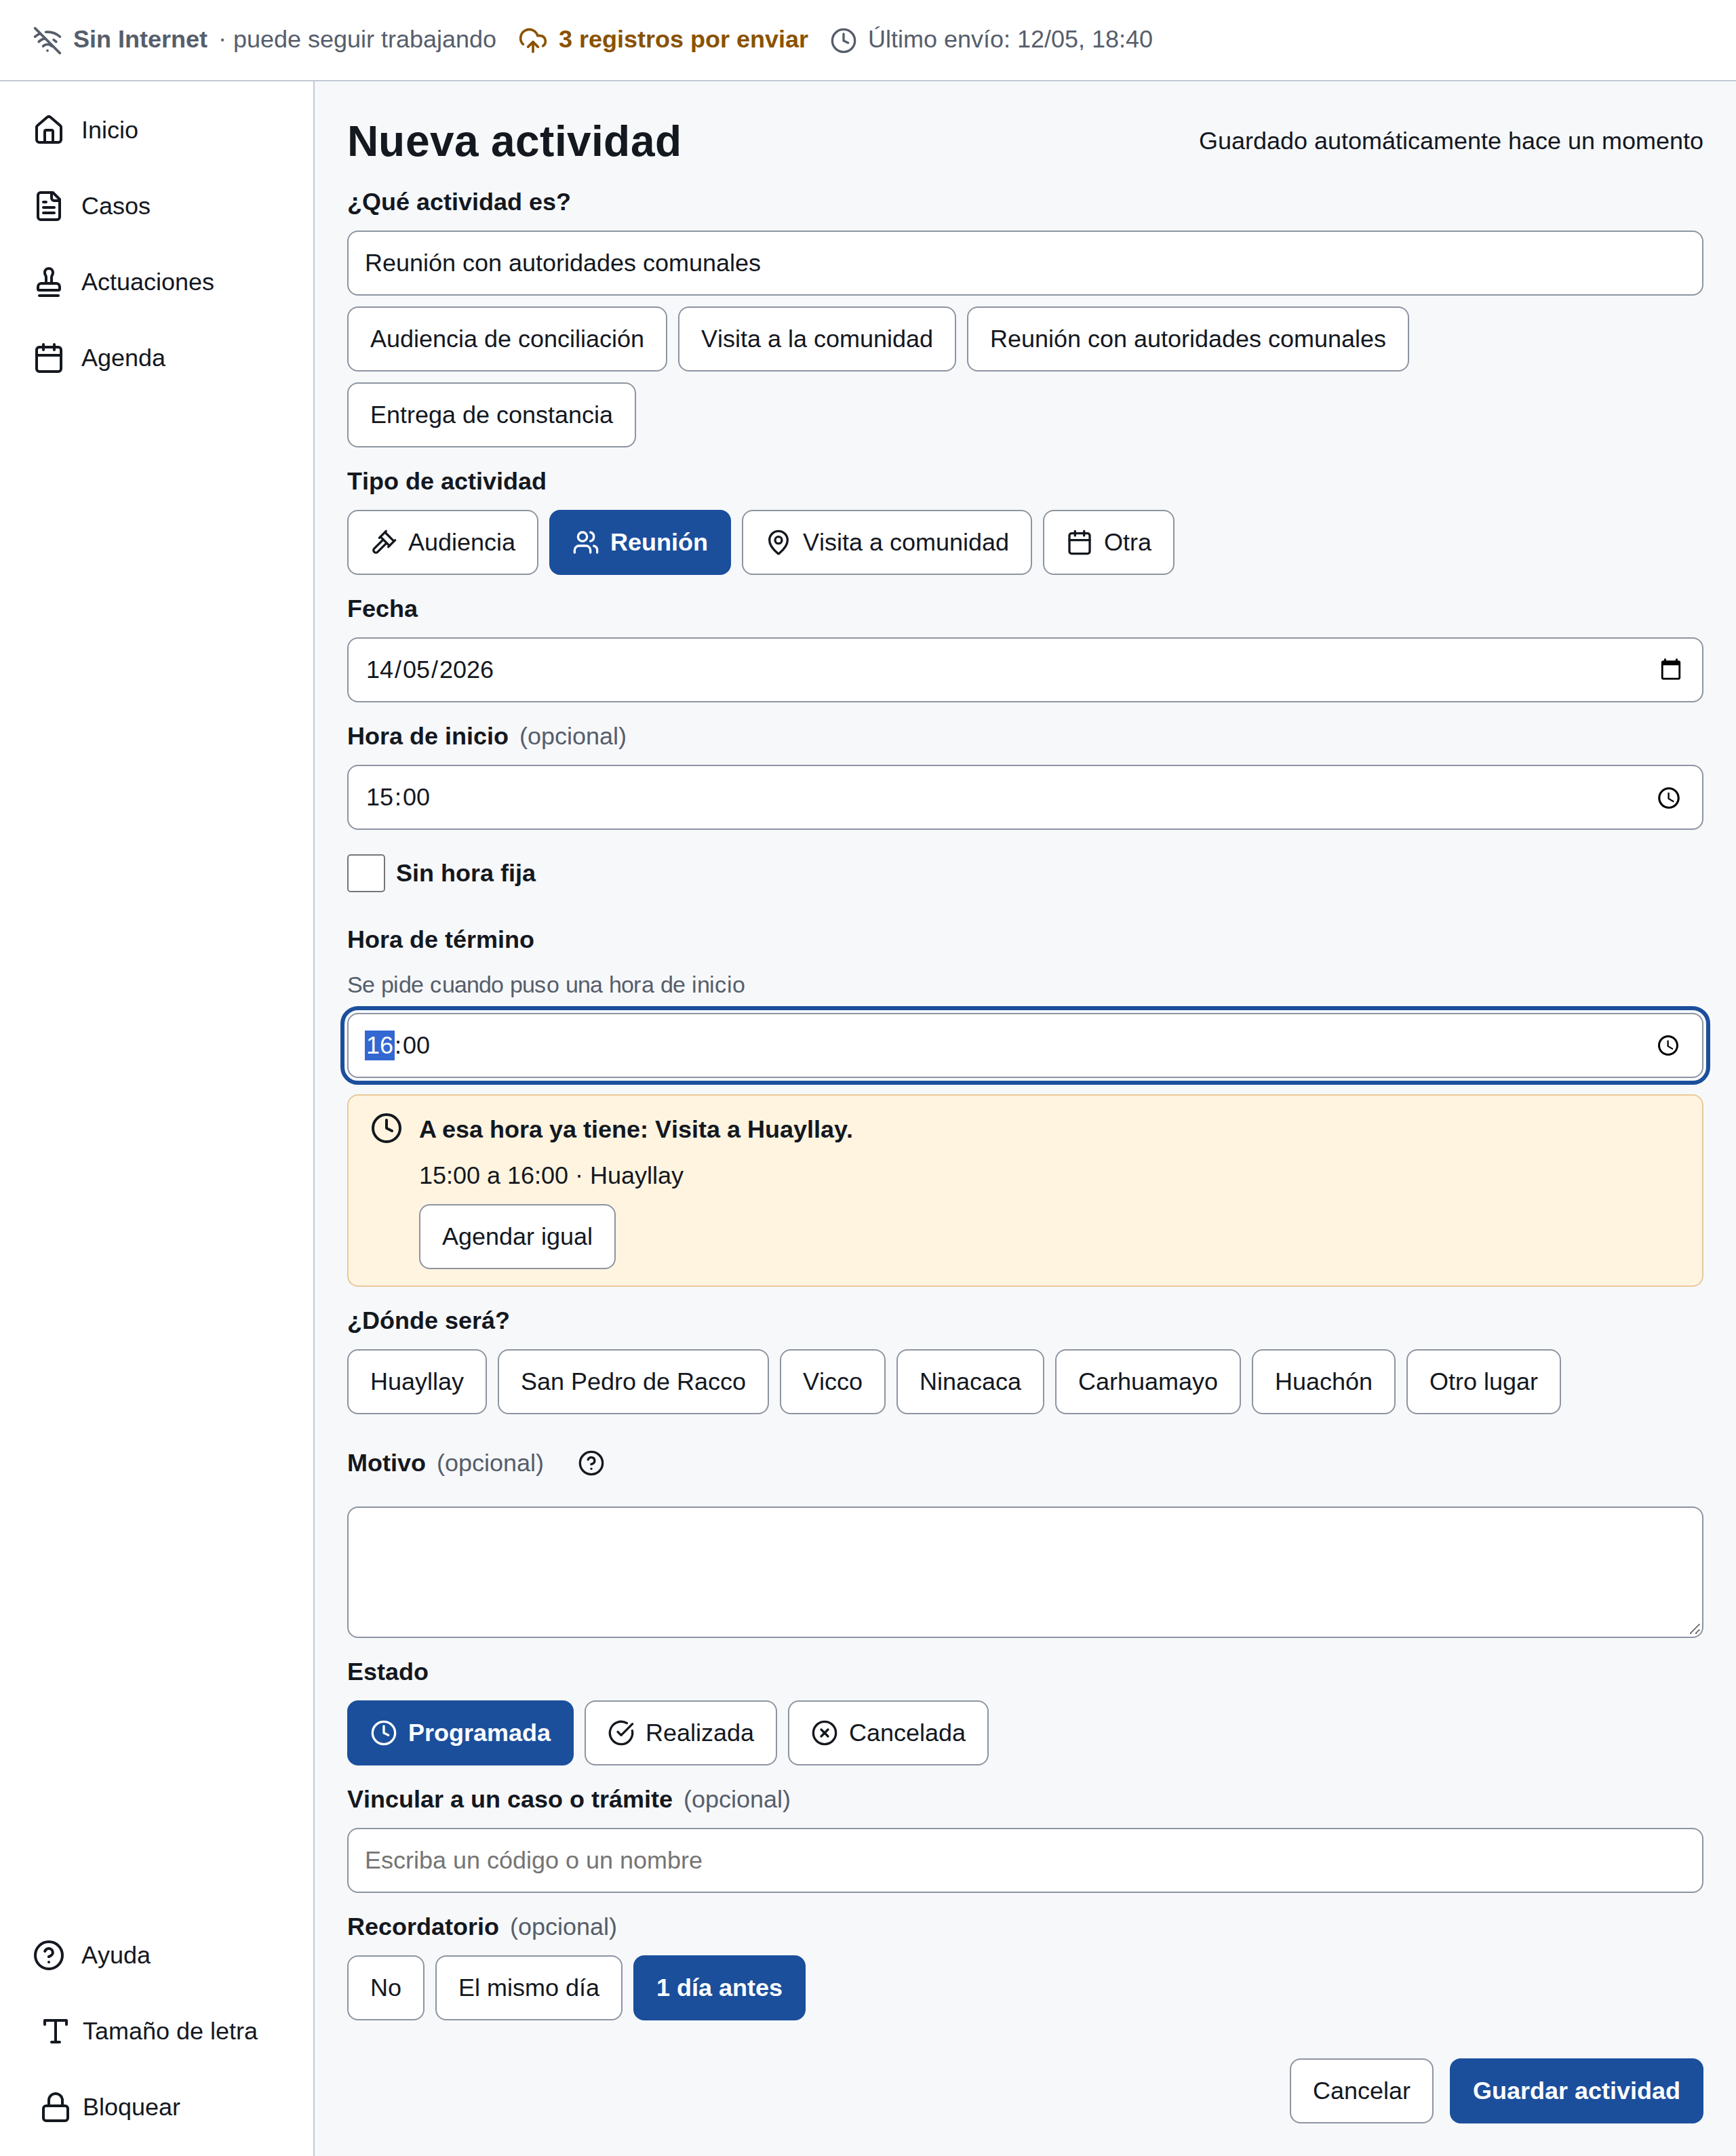
\includegraphics[width=0.82\linewidth]{capturas/F4-01_cruce-horario.png}
\caption{P-08 · 2. Aviso de cruce de horario. Avisa qué actividad choca a esa hora, sin bloquear}
\end{figure}
\begin{figure}[H]\centering
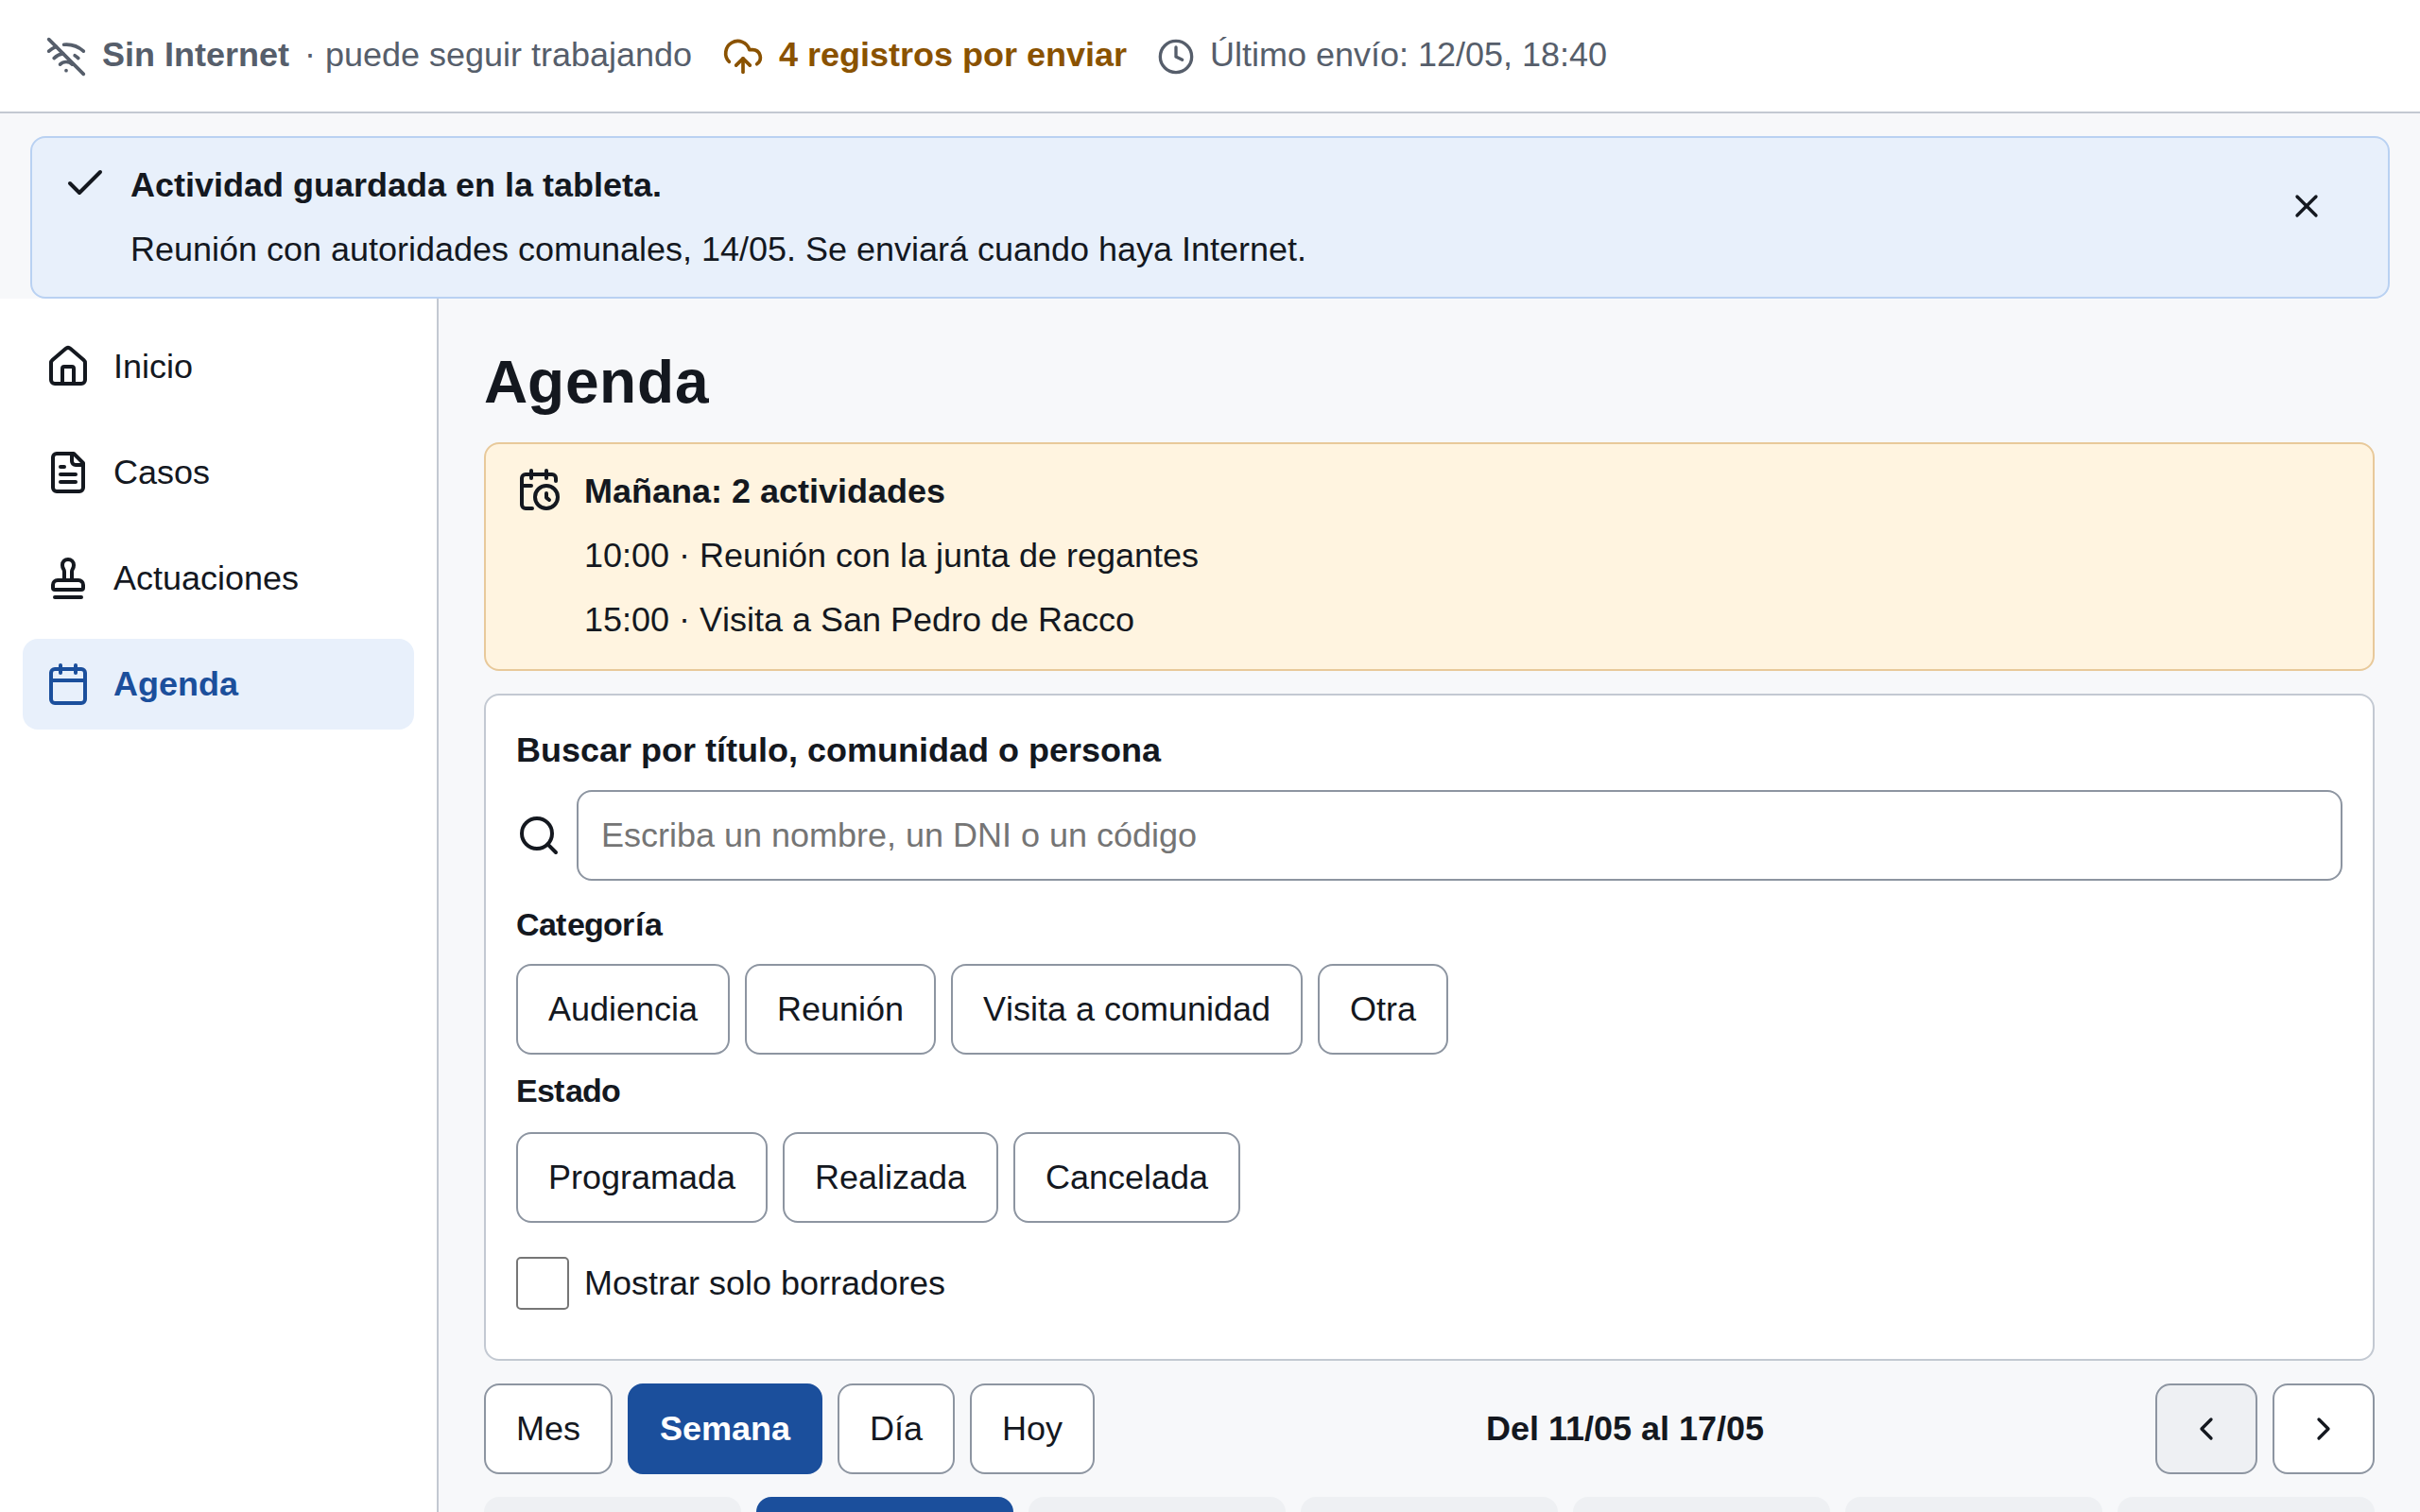
\includegraphics[width=0.82\linewidth]{capturas/F4-02_guardada.png}
\caption{P-07 · 3. Actividad guardada en la tableta. Confirmación de guardado local y contador de la barra en 4}
\end{figure}
\begin{figure}[H]\centering
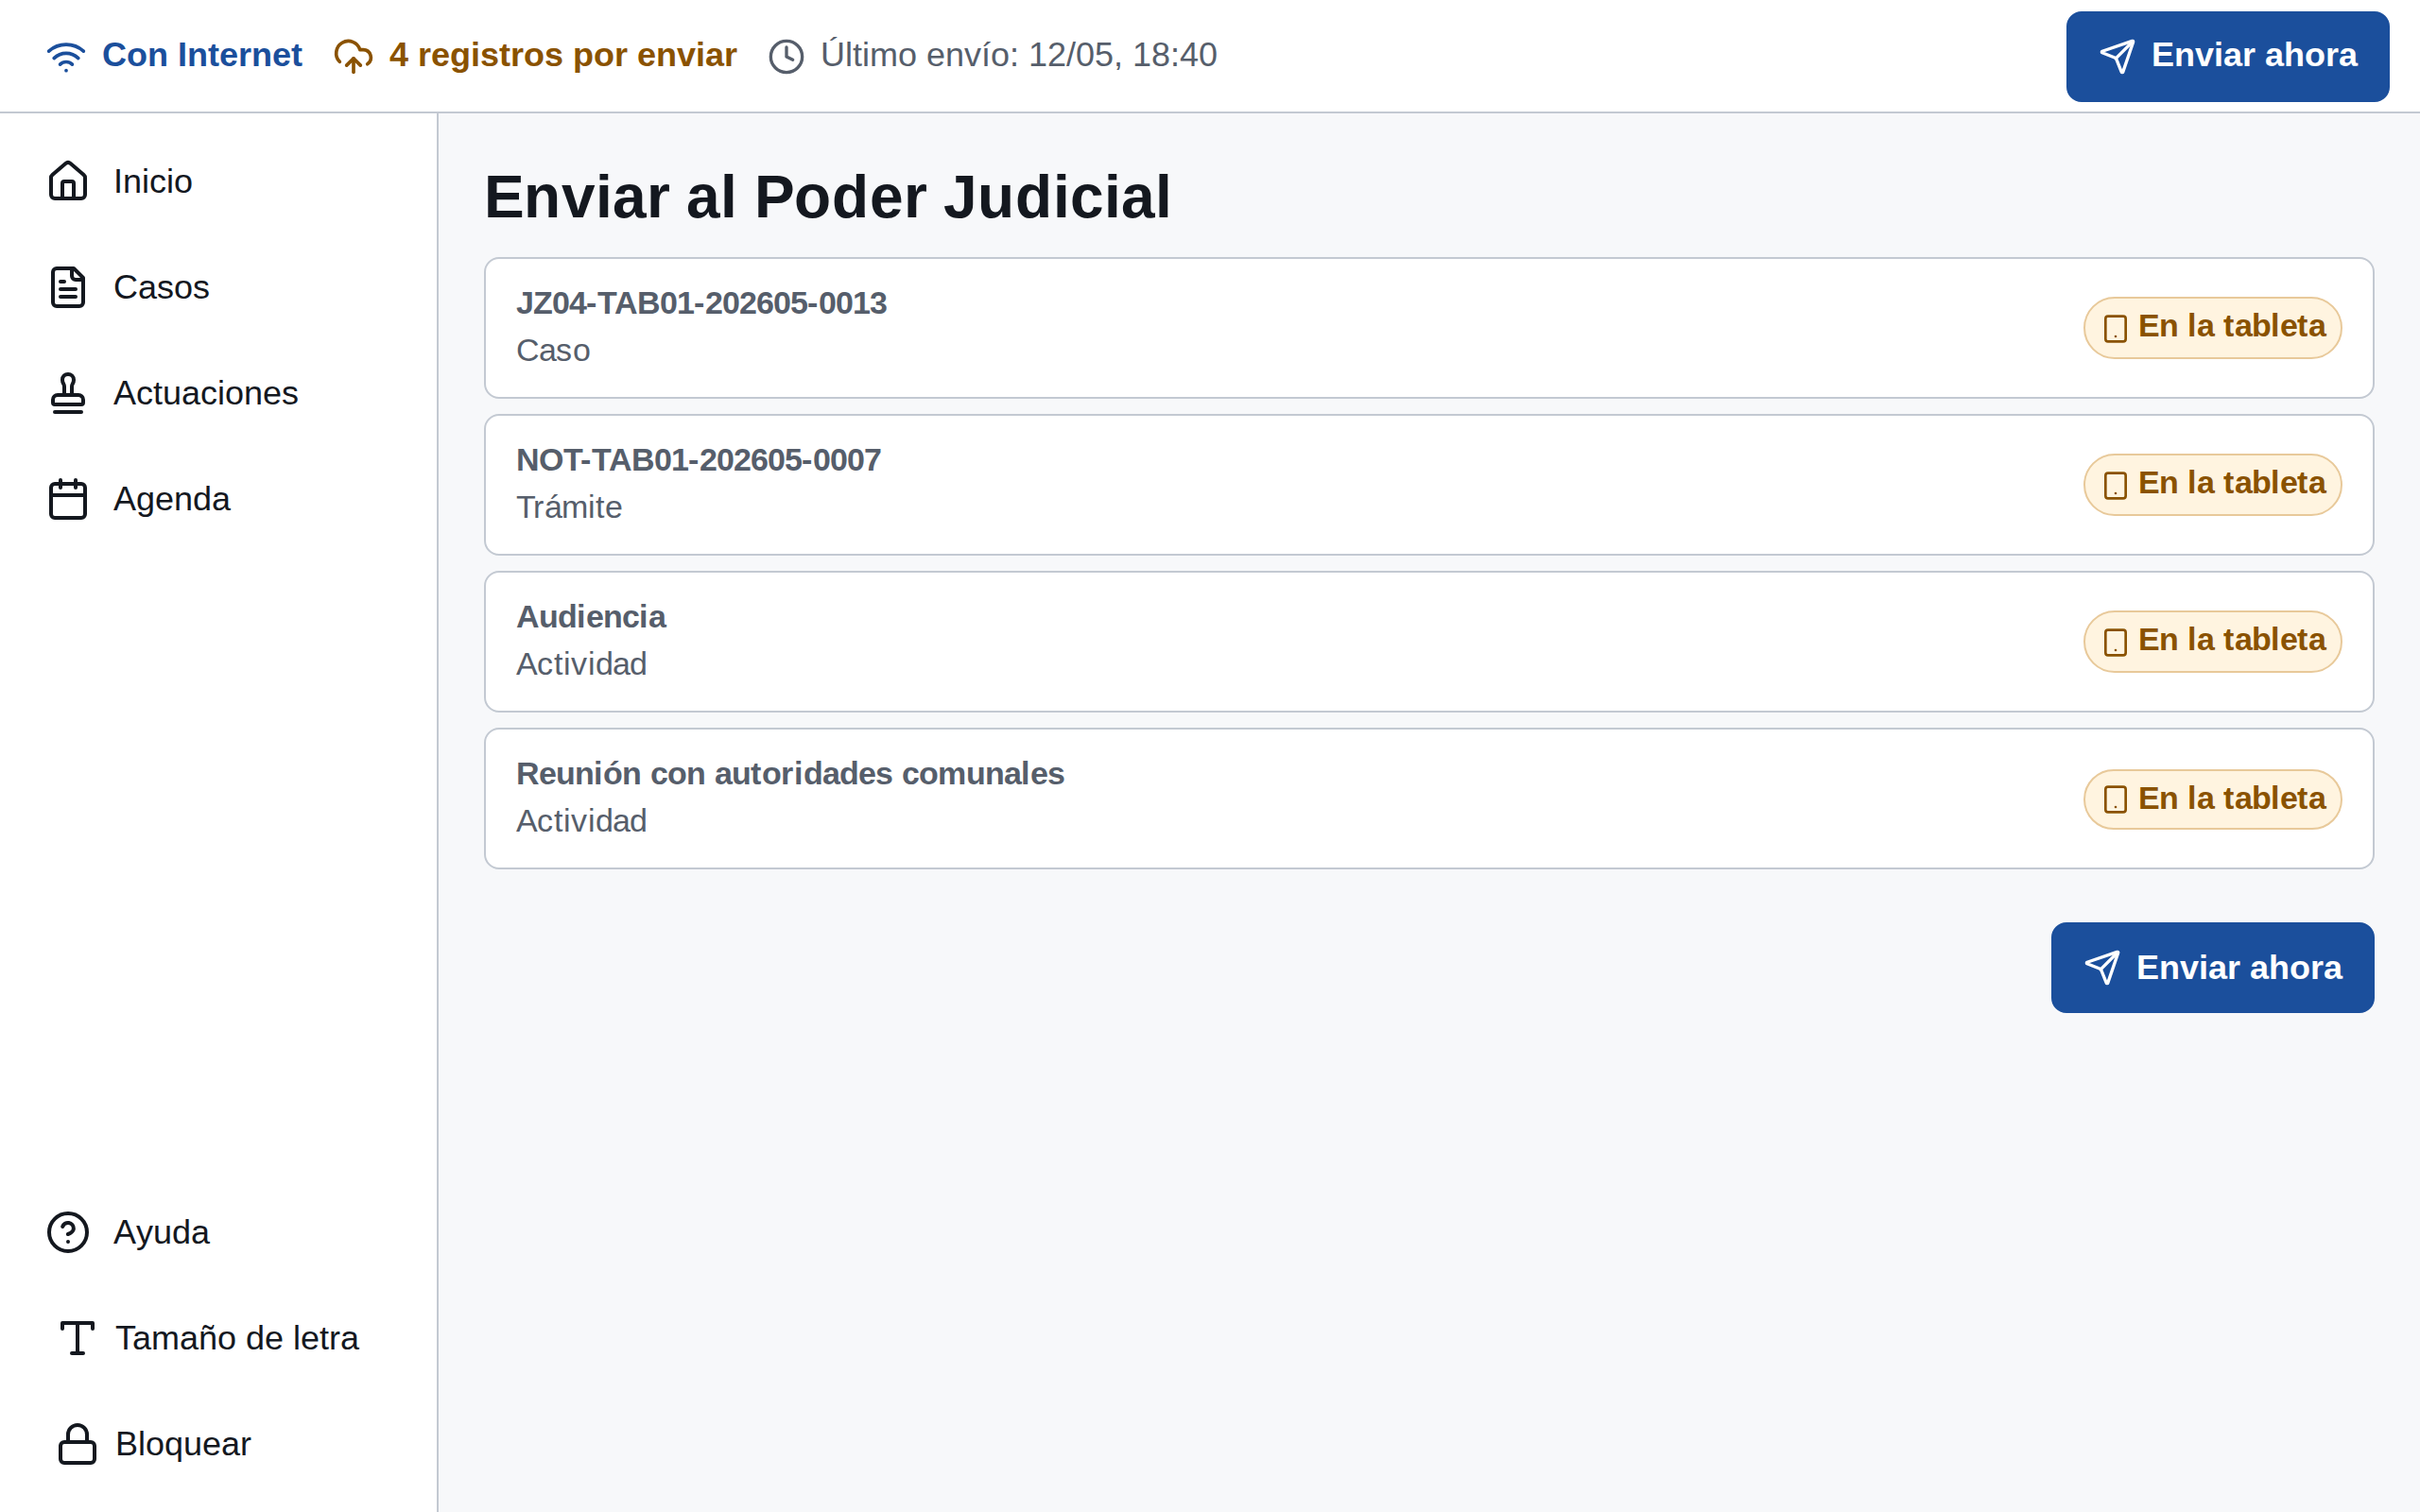
\includegraphics[width=0.82\linewidth]{capturas/F4-03_vuelve-internet.png}
\caption{P-09 · 4. Vuelve el Internet. Con Internet aparece el botón Enviar ahora en la barra y en la pantalla}
\end{figure}
\begin{figure}[H]\centering
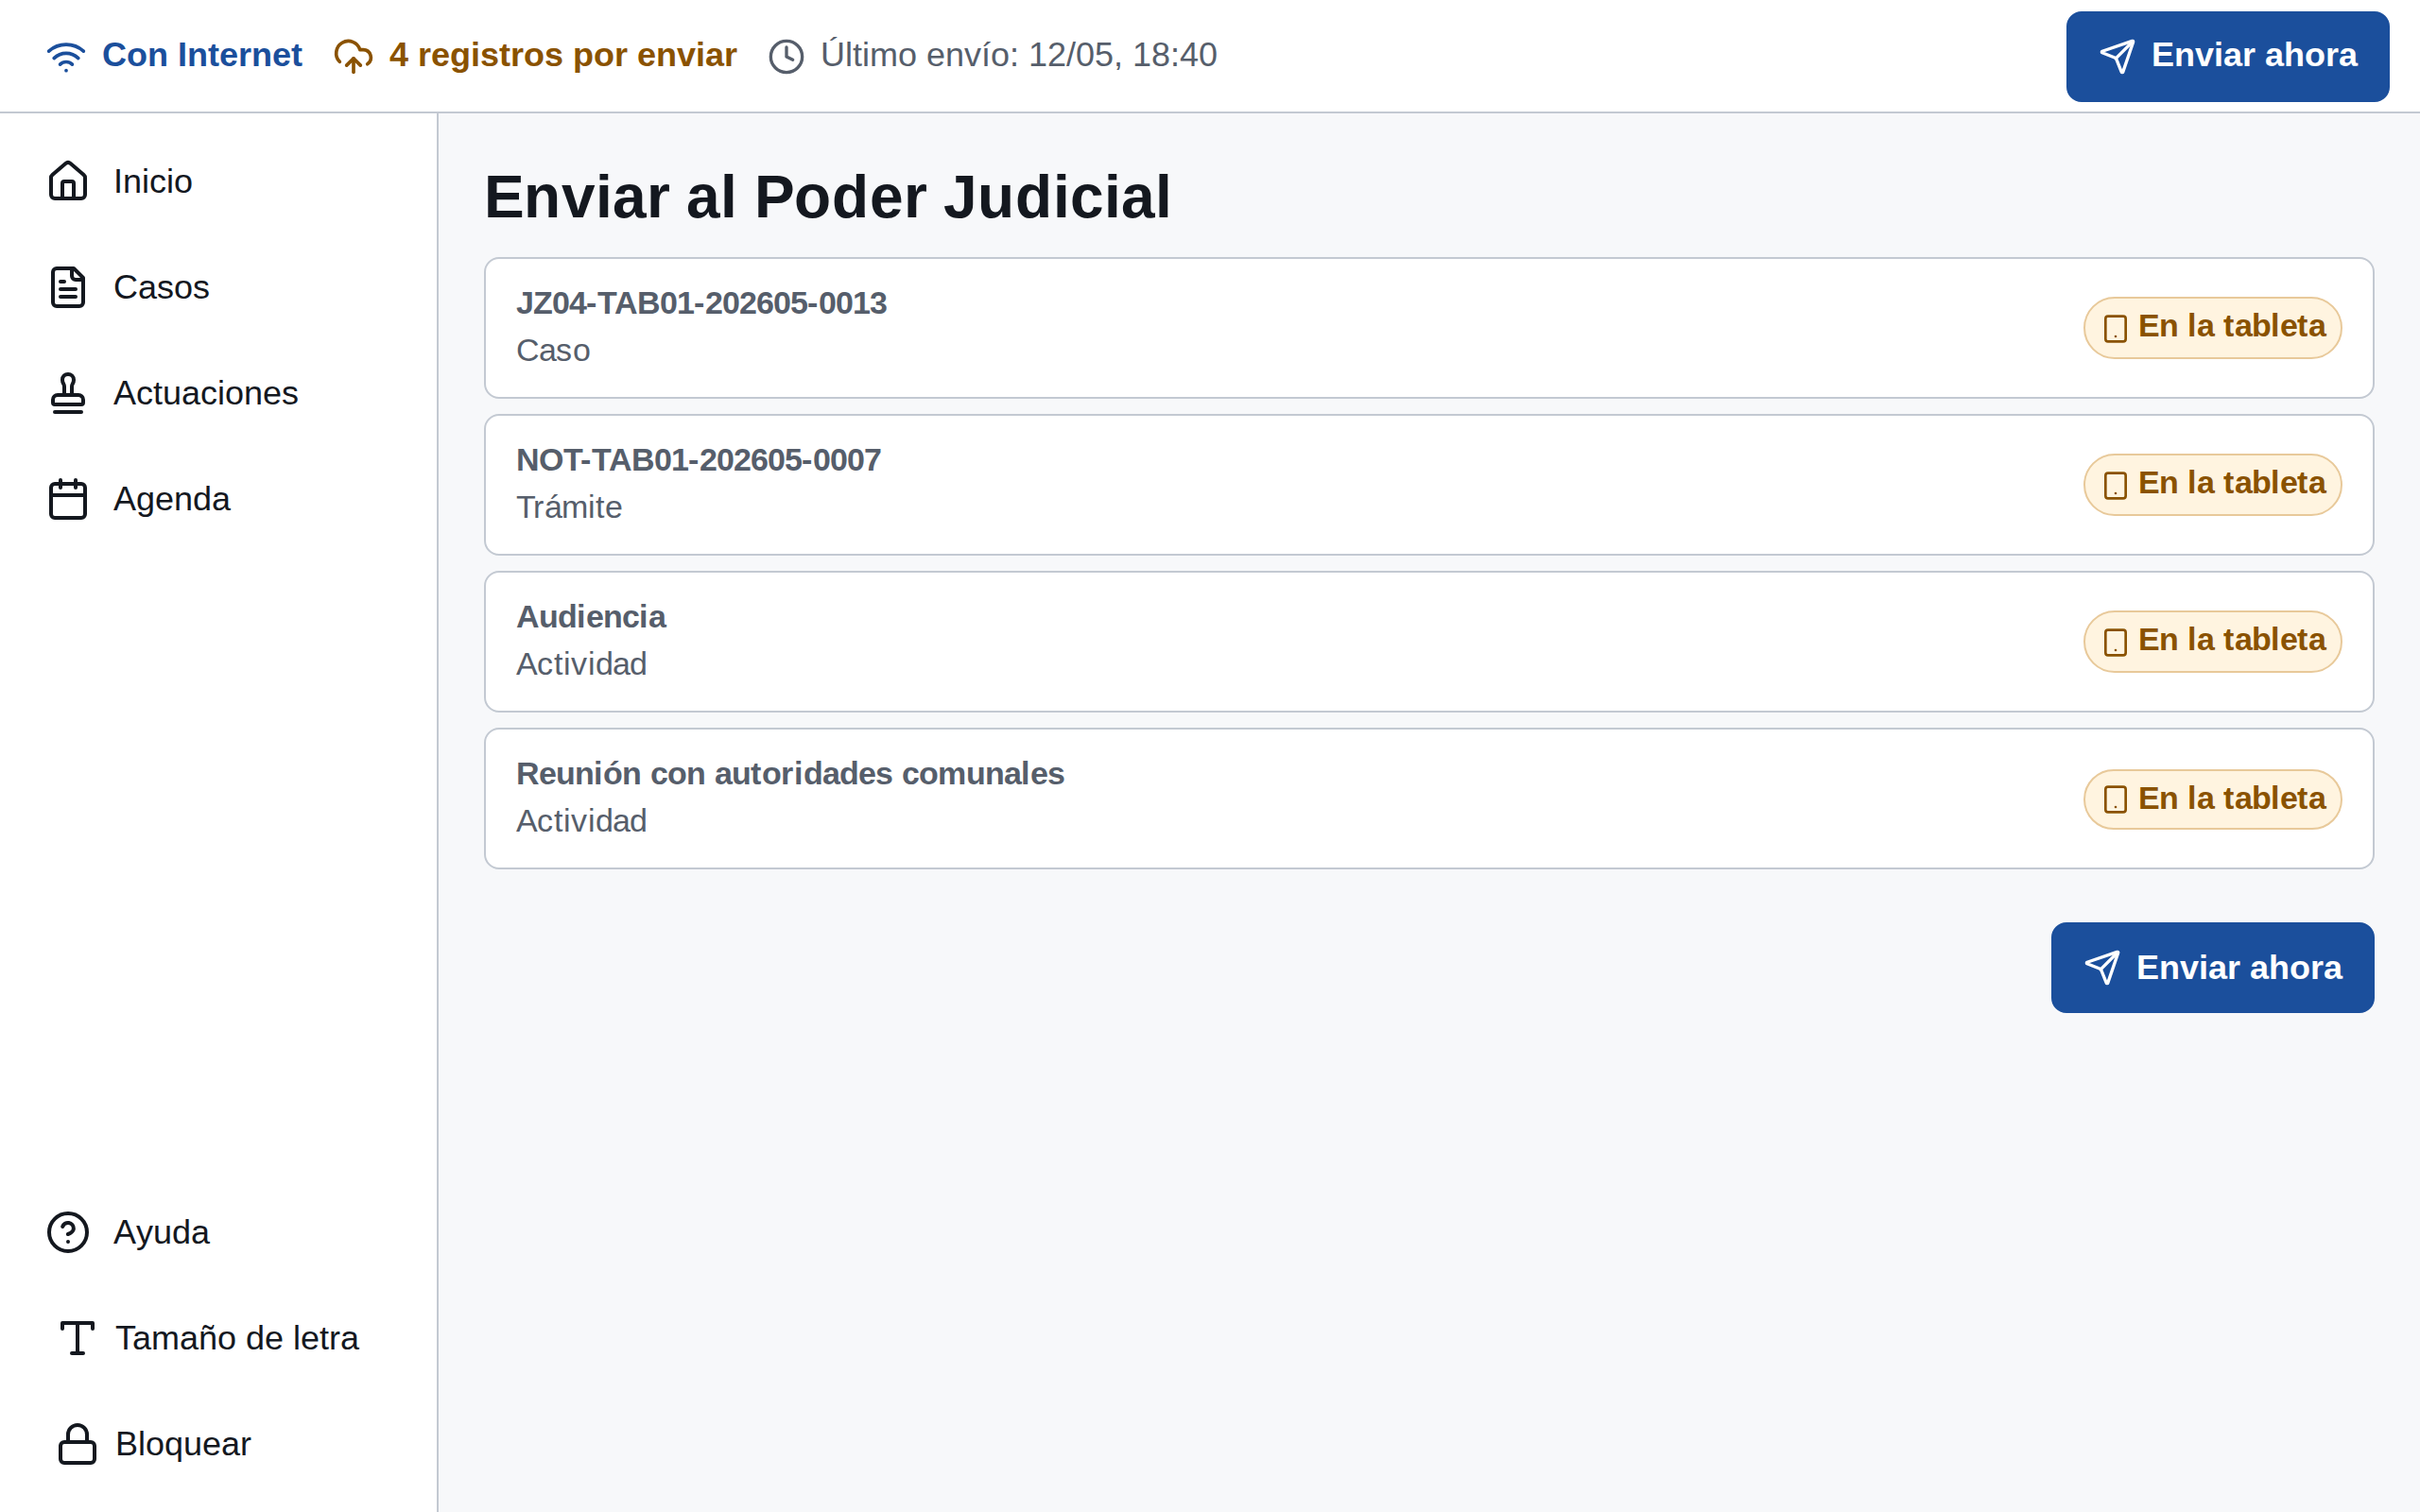
\includegraphics[width=0.82\linewidth]{capturas/F4-04_pendientes-del-dia.png}
\caption{P-09 · 5. Los cuatro registros del día. La pantalla de envío lista lo que la jueza registró en el día: el caso, su audiencia, el trámite y la reunión}
\end{figure}
\begin{figure}[H]\centering
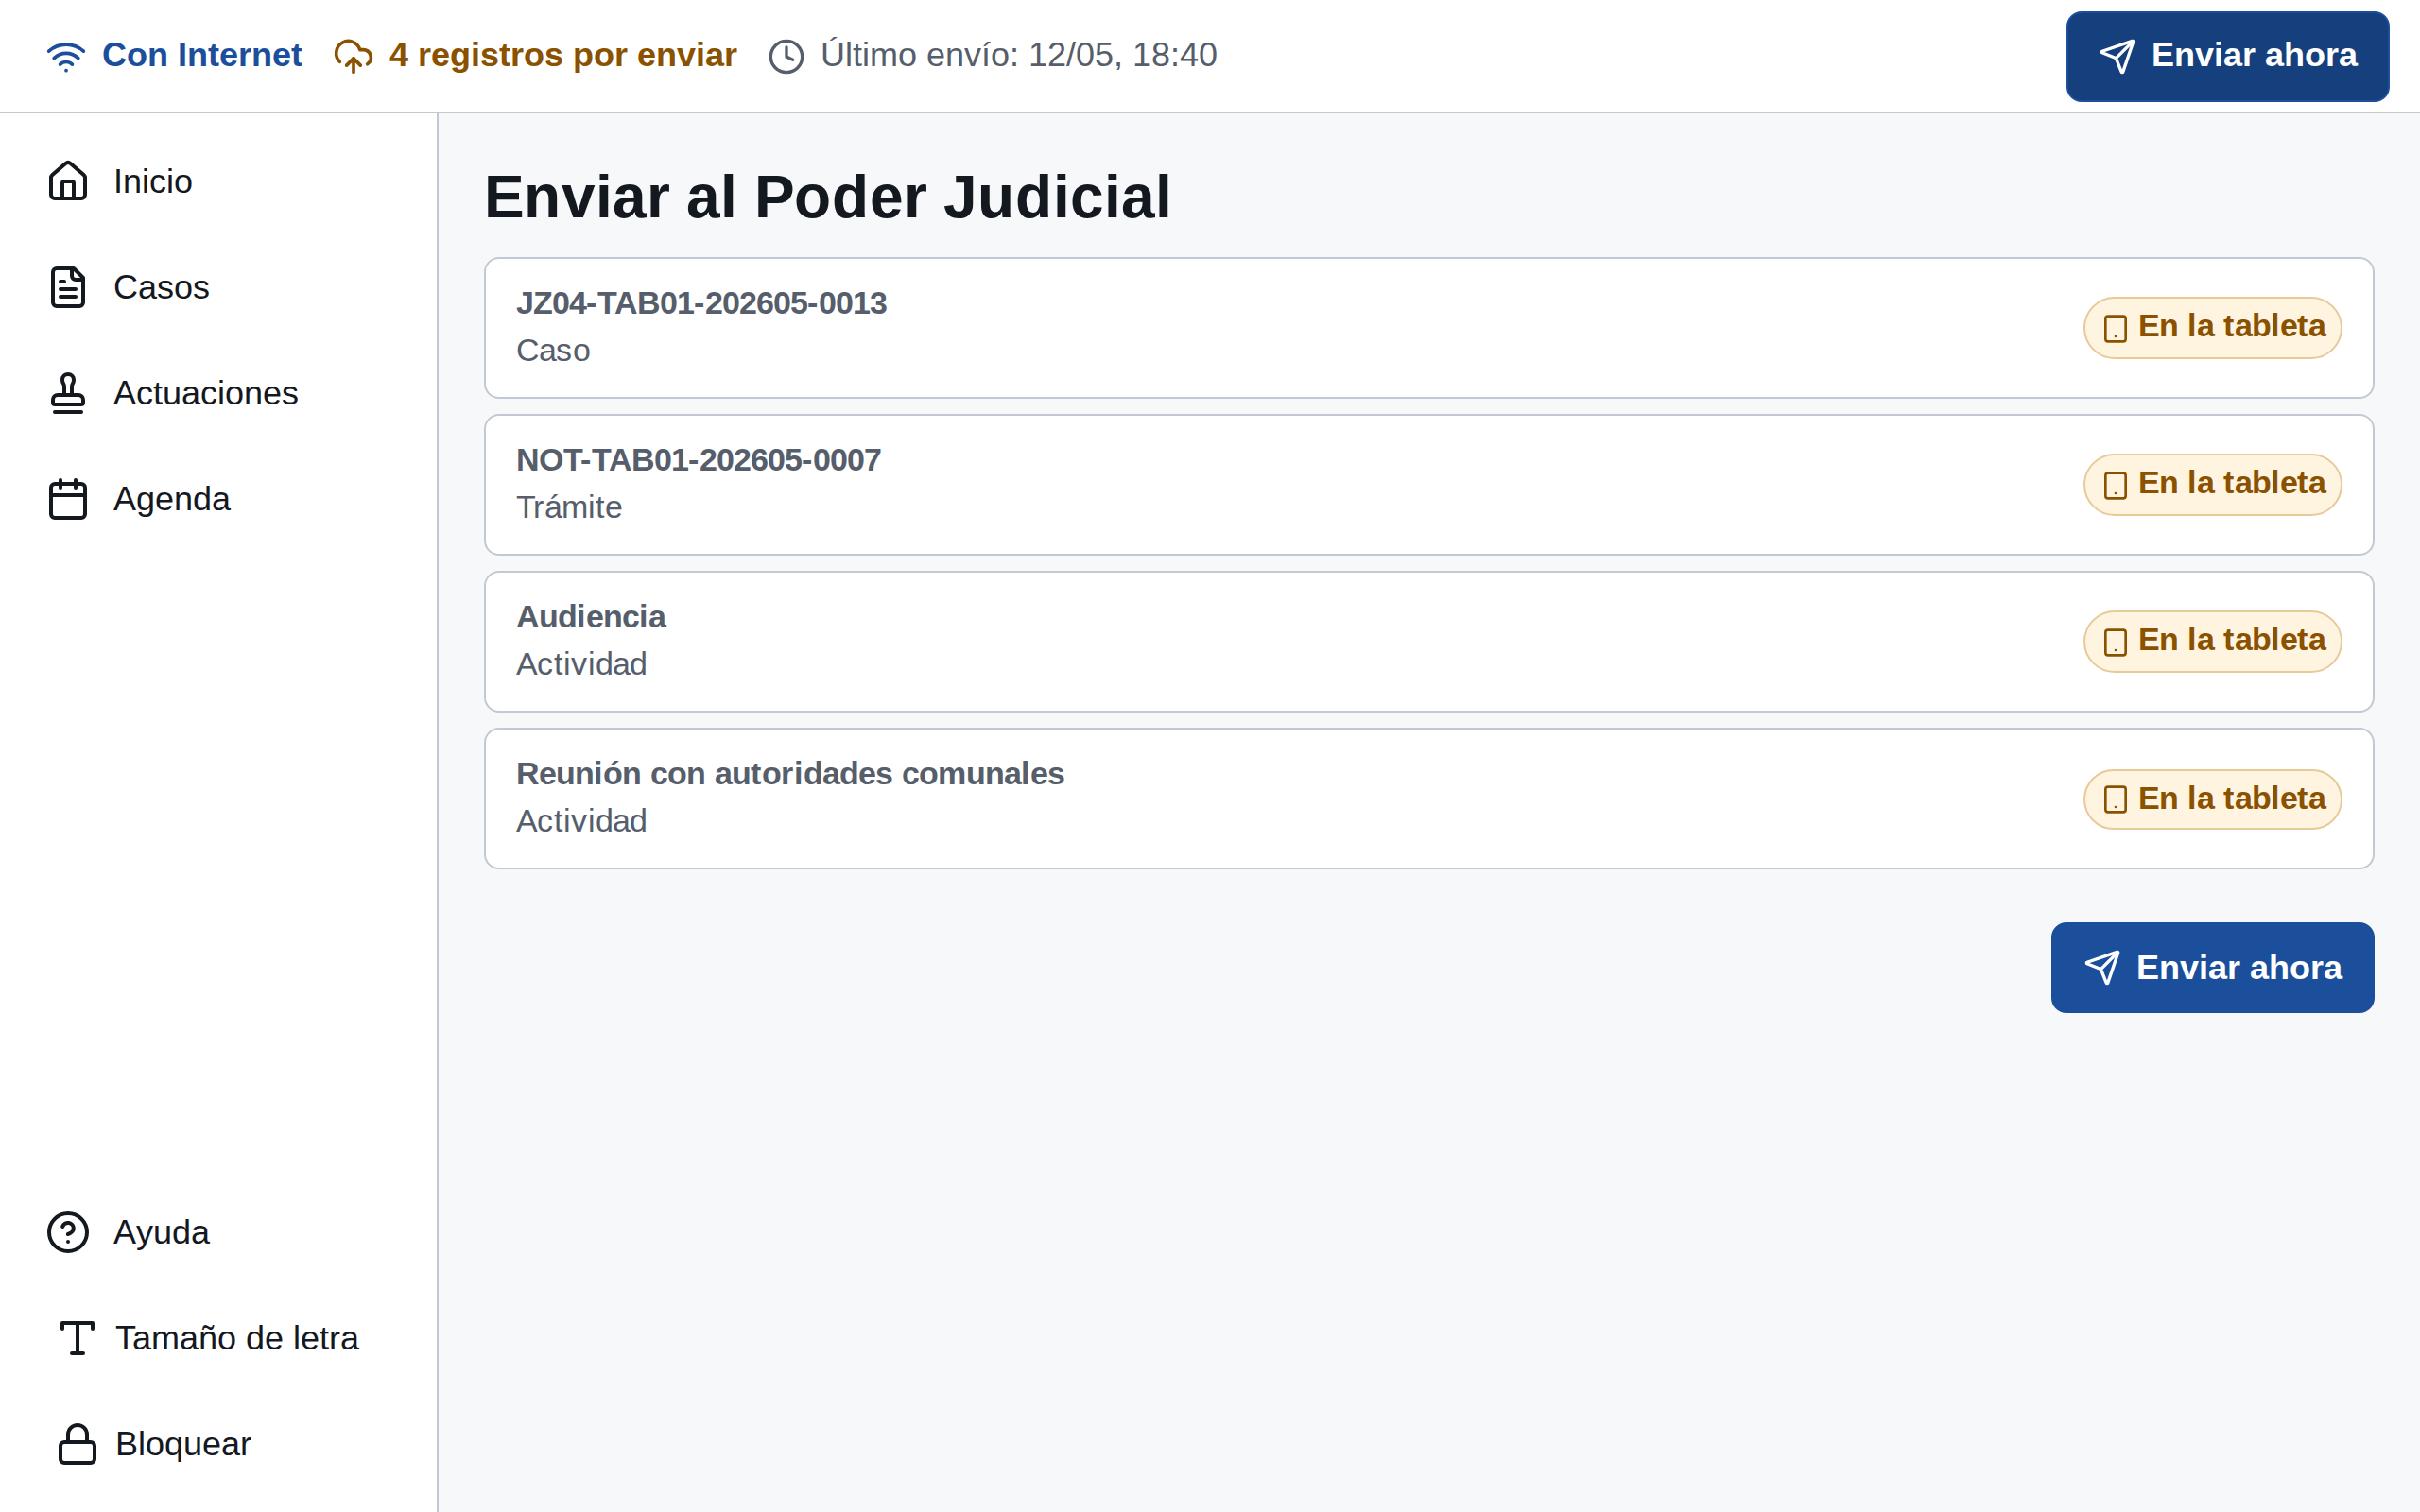
\includegraphics[width=0.82\linewidth]{capturas/F4-04b_progreso.png}
\caption{P-09 · 6. Enviando. Progreso del envío de los cuatro registros del día}
\end{figure}
\begin{figure}[H]\centering
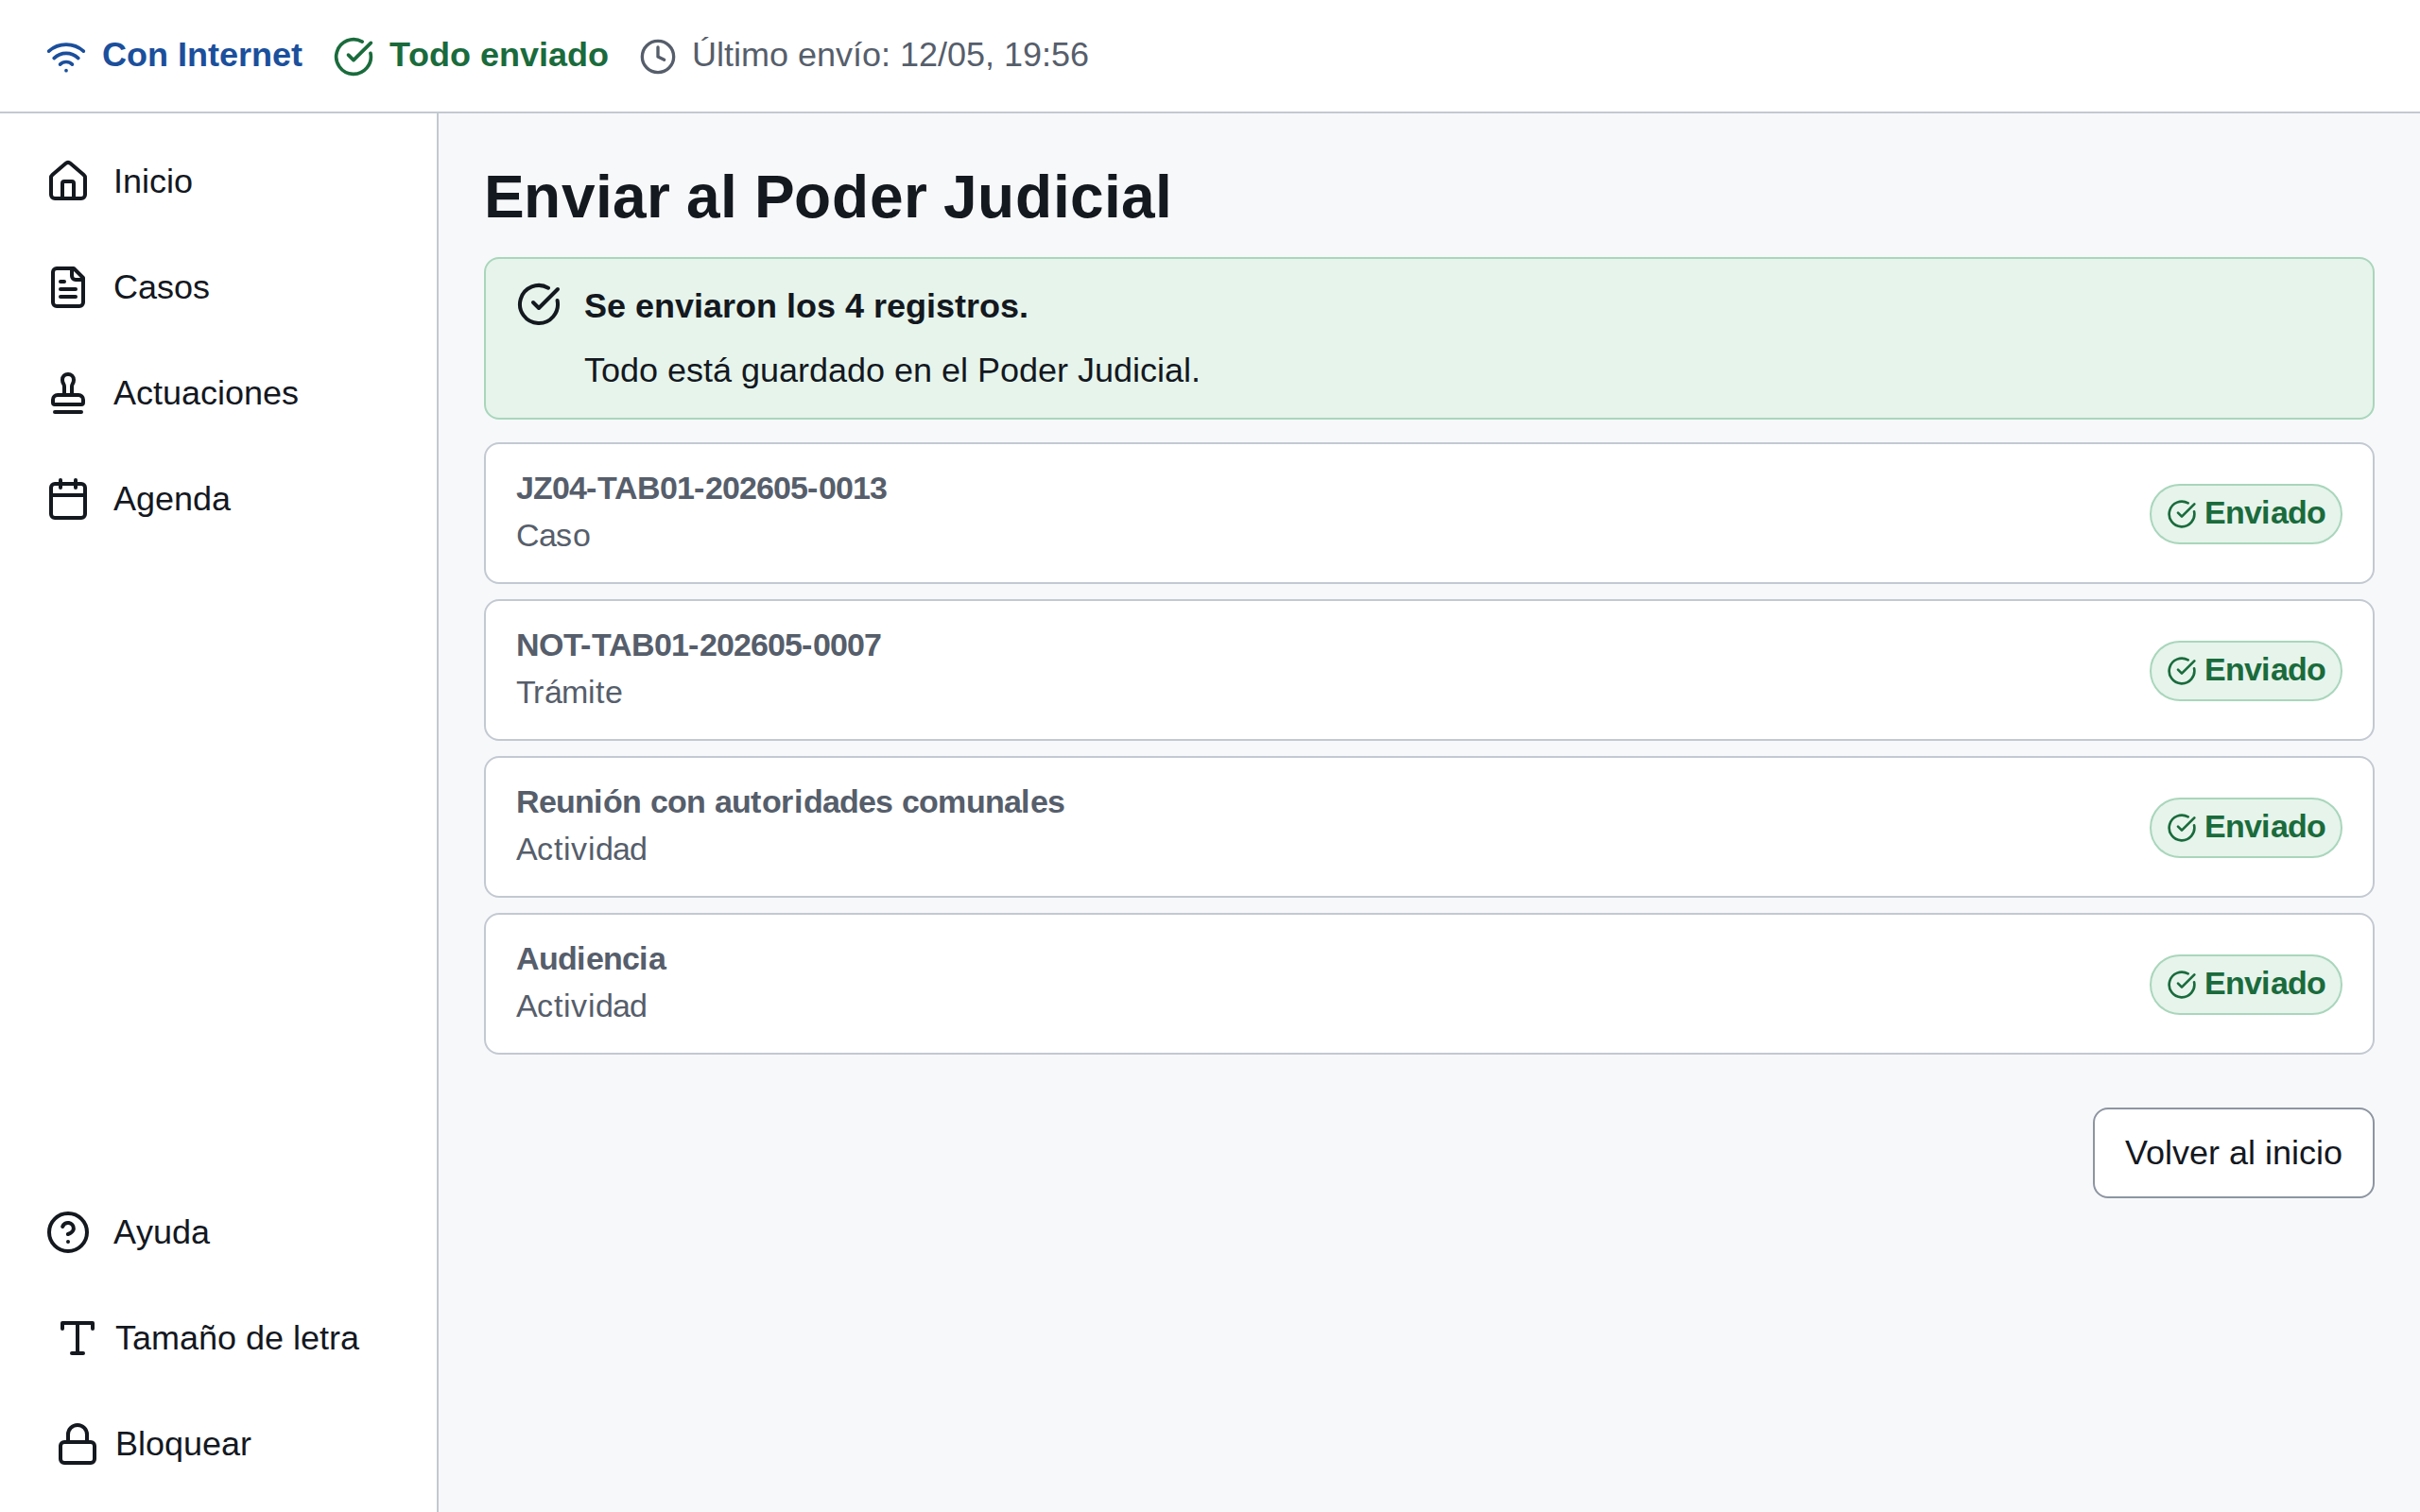
\includegraphics[width=0.82\linewidth]{capturas/F4-05_exito.png}
\caption{P-09 · 7. Envío completo. Se enviaron los 4 registros del día y la barra pasa a Todo enviado}
\end{figure}
\subsection{Flujo complementario A · Actualizar el avance de un caso}
\begin{figure}[H]\centering
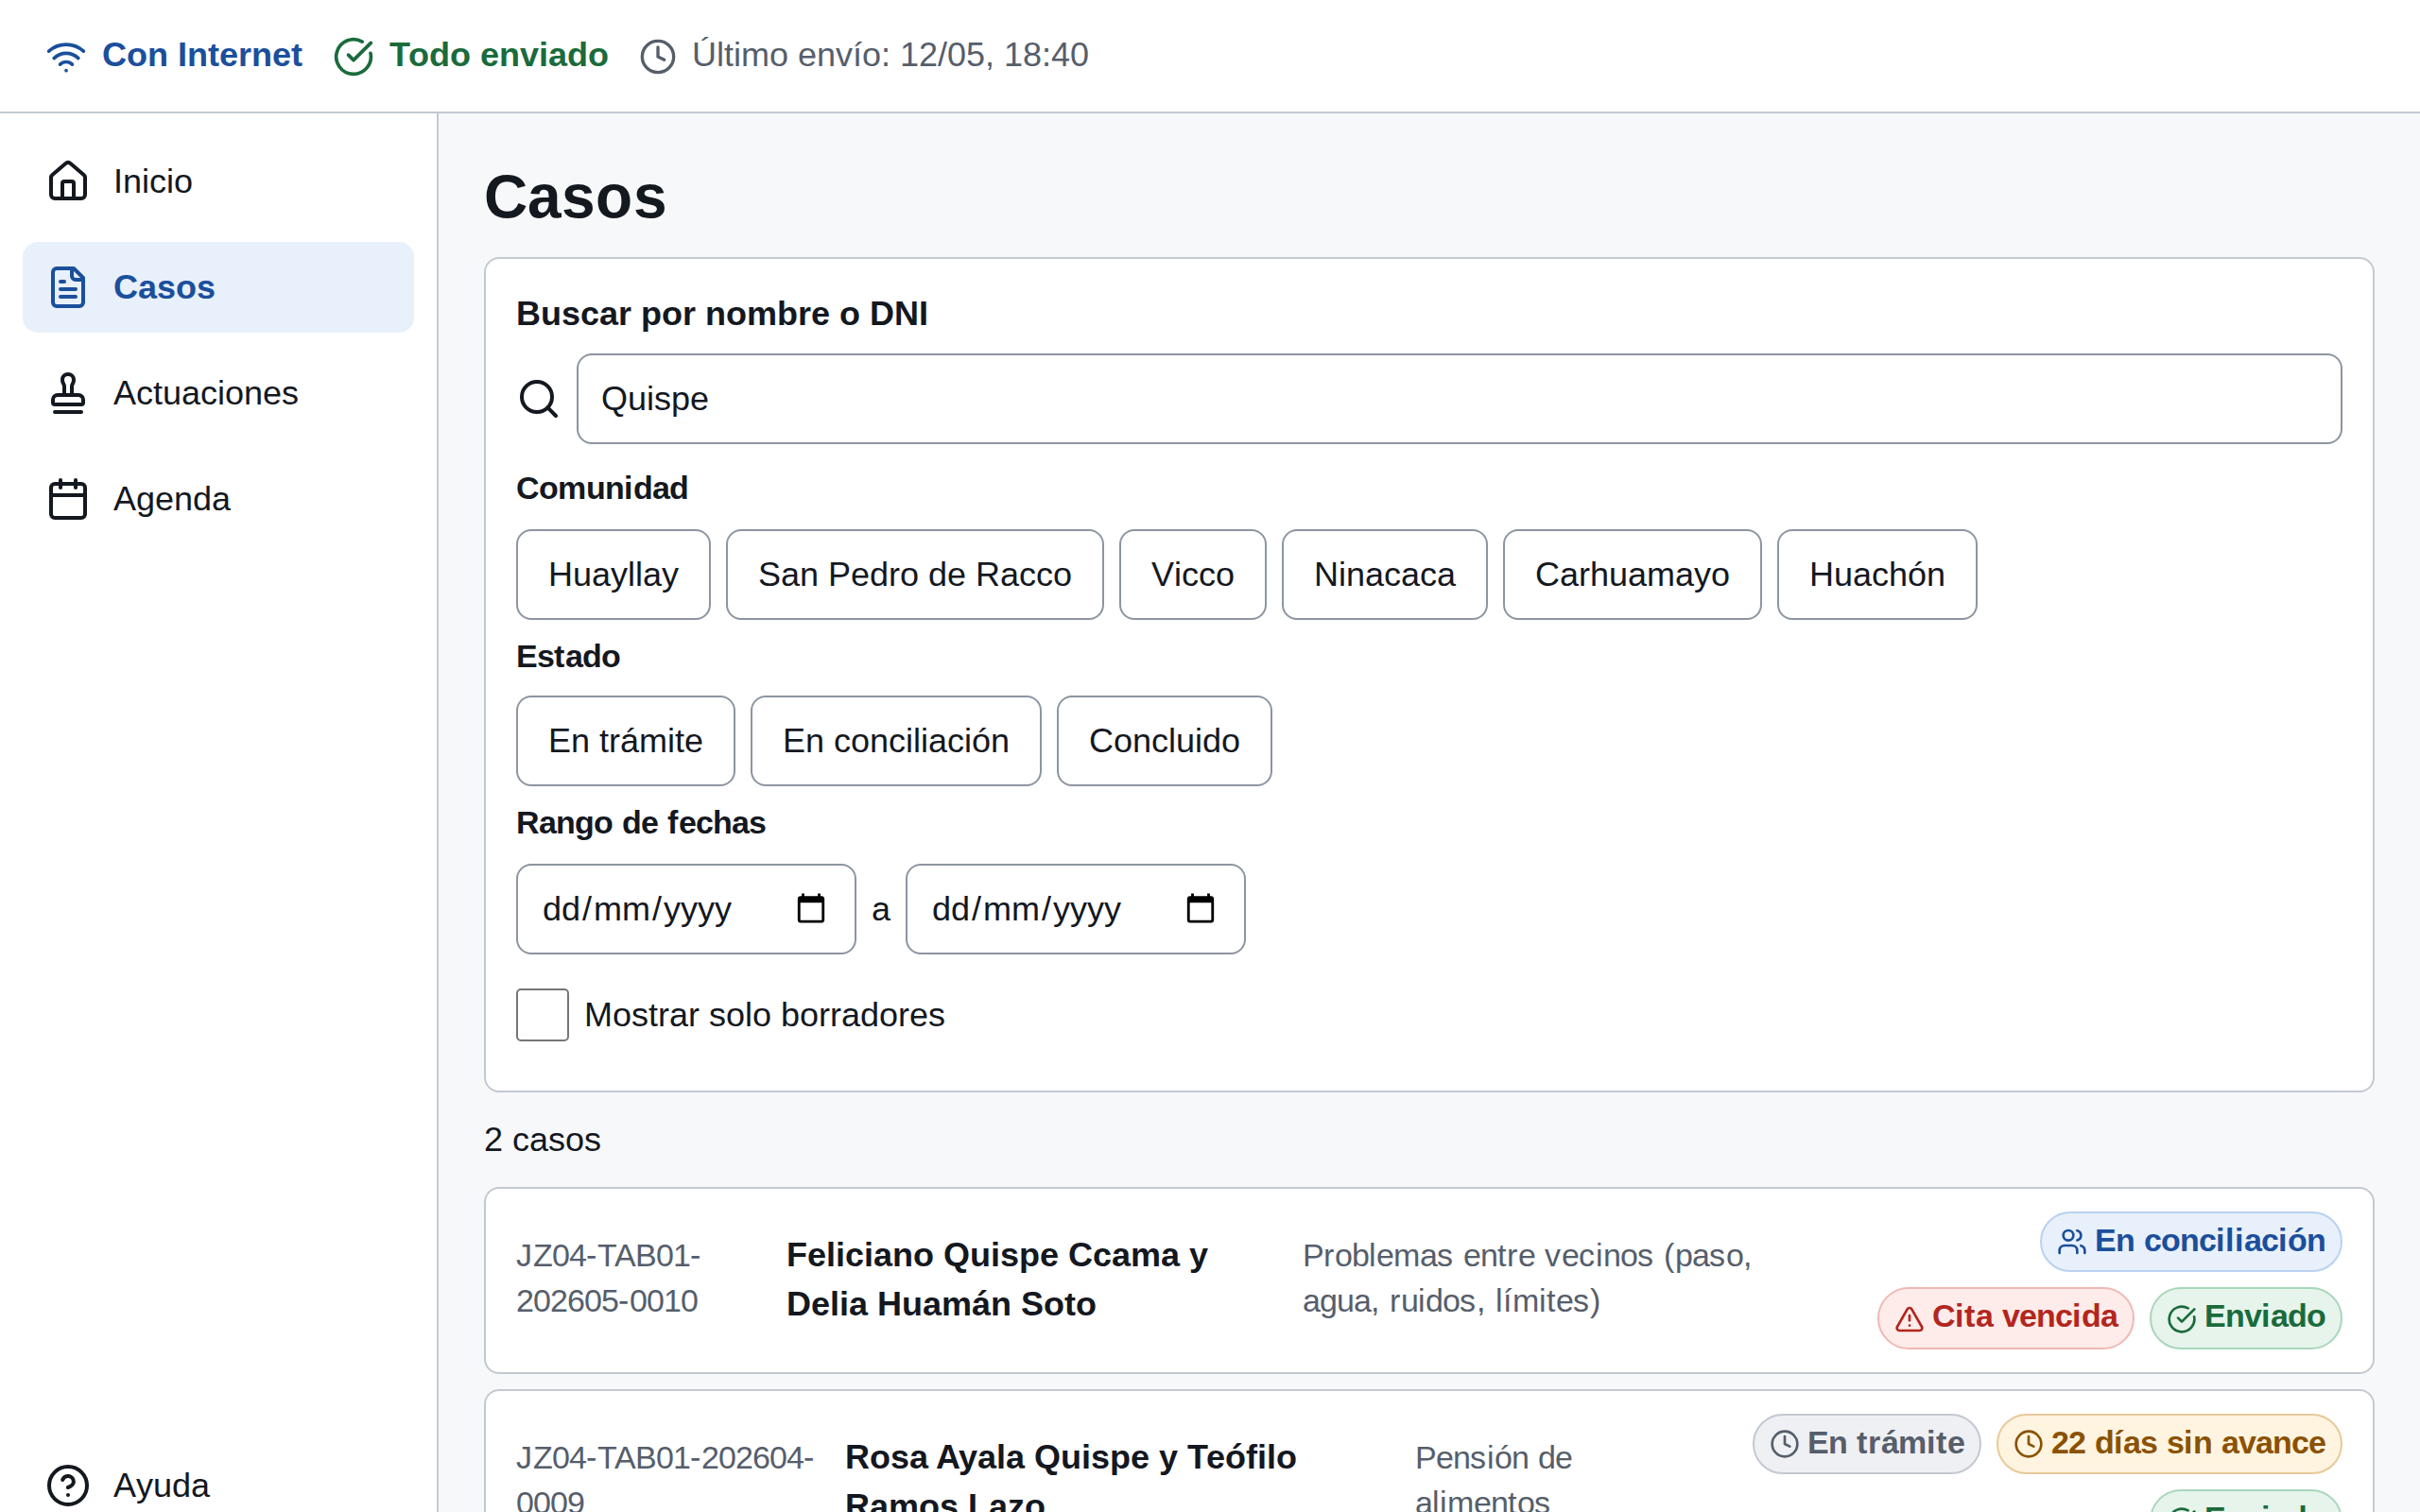
\includegraphics[width=0.82\linewidth]{capturas/FA-01_busqueda.png}
\caption{P-02 · 1. Búsqueda y filtros. Un solo campo busca por nombre o DNI; los filtros son botones visibles}
\end{figure}
\begin{figure}[H]\centering
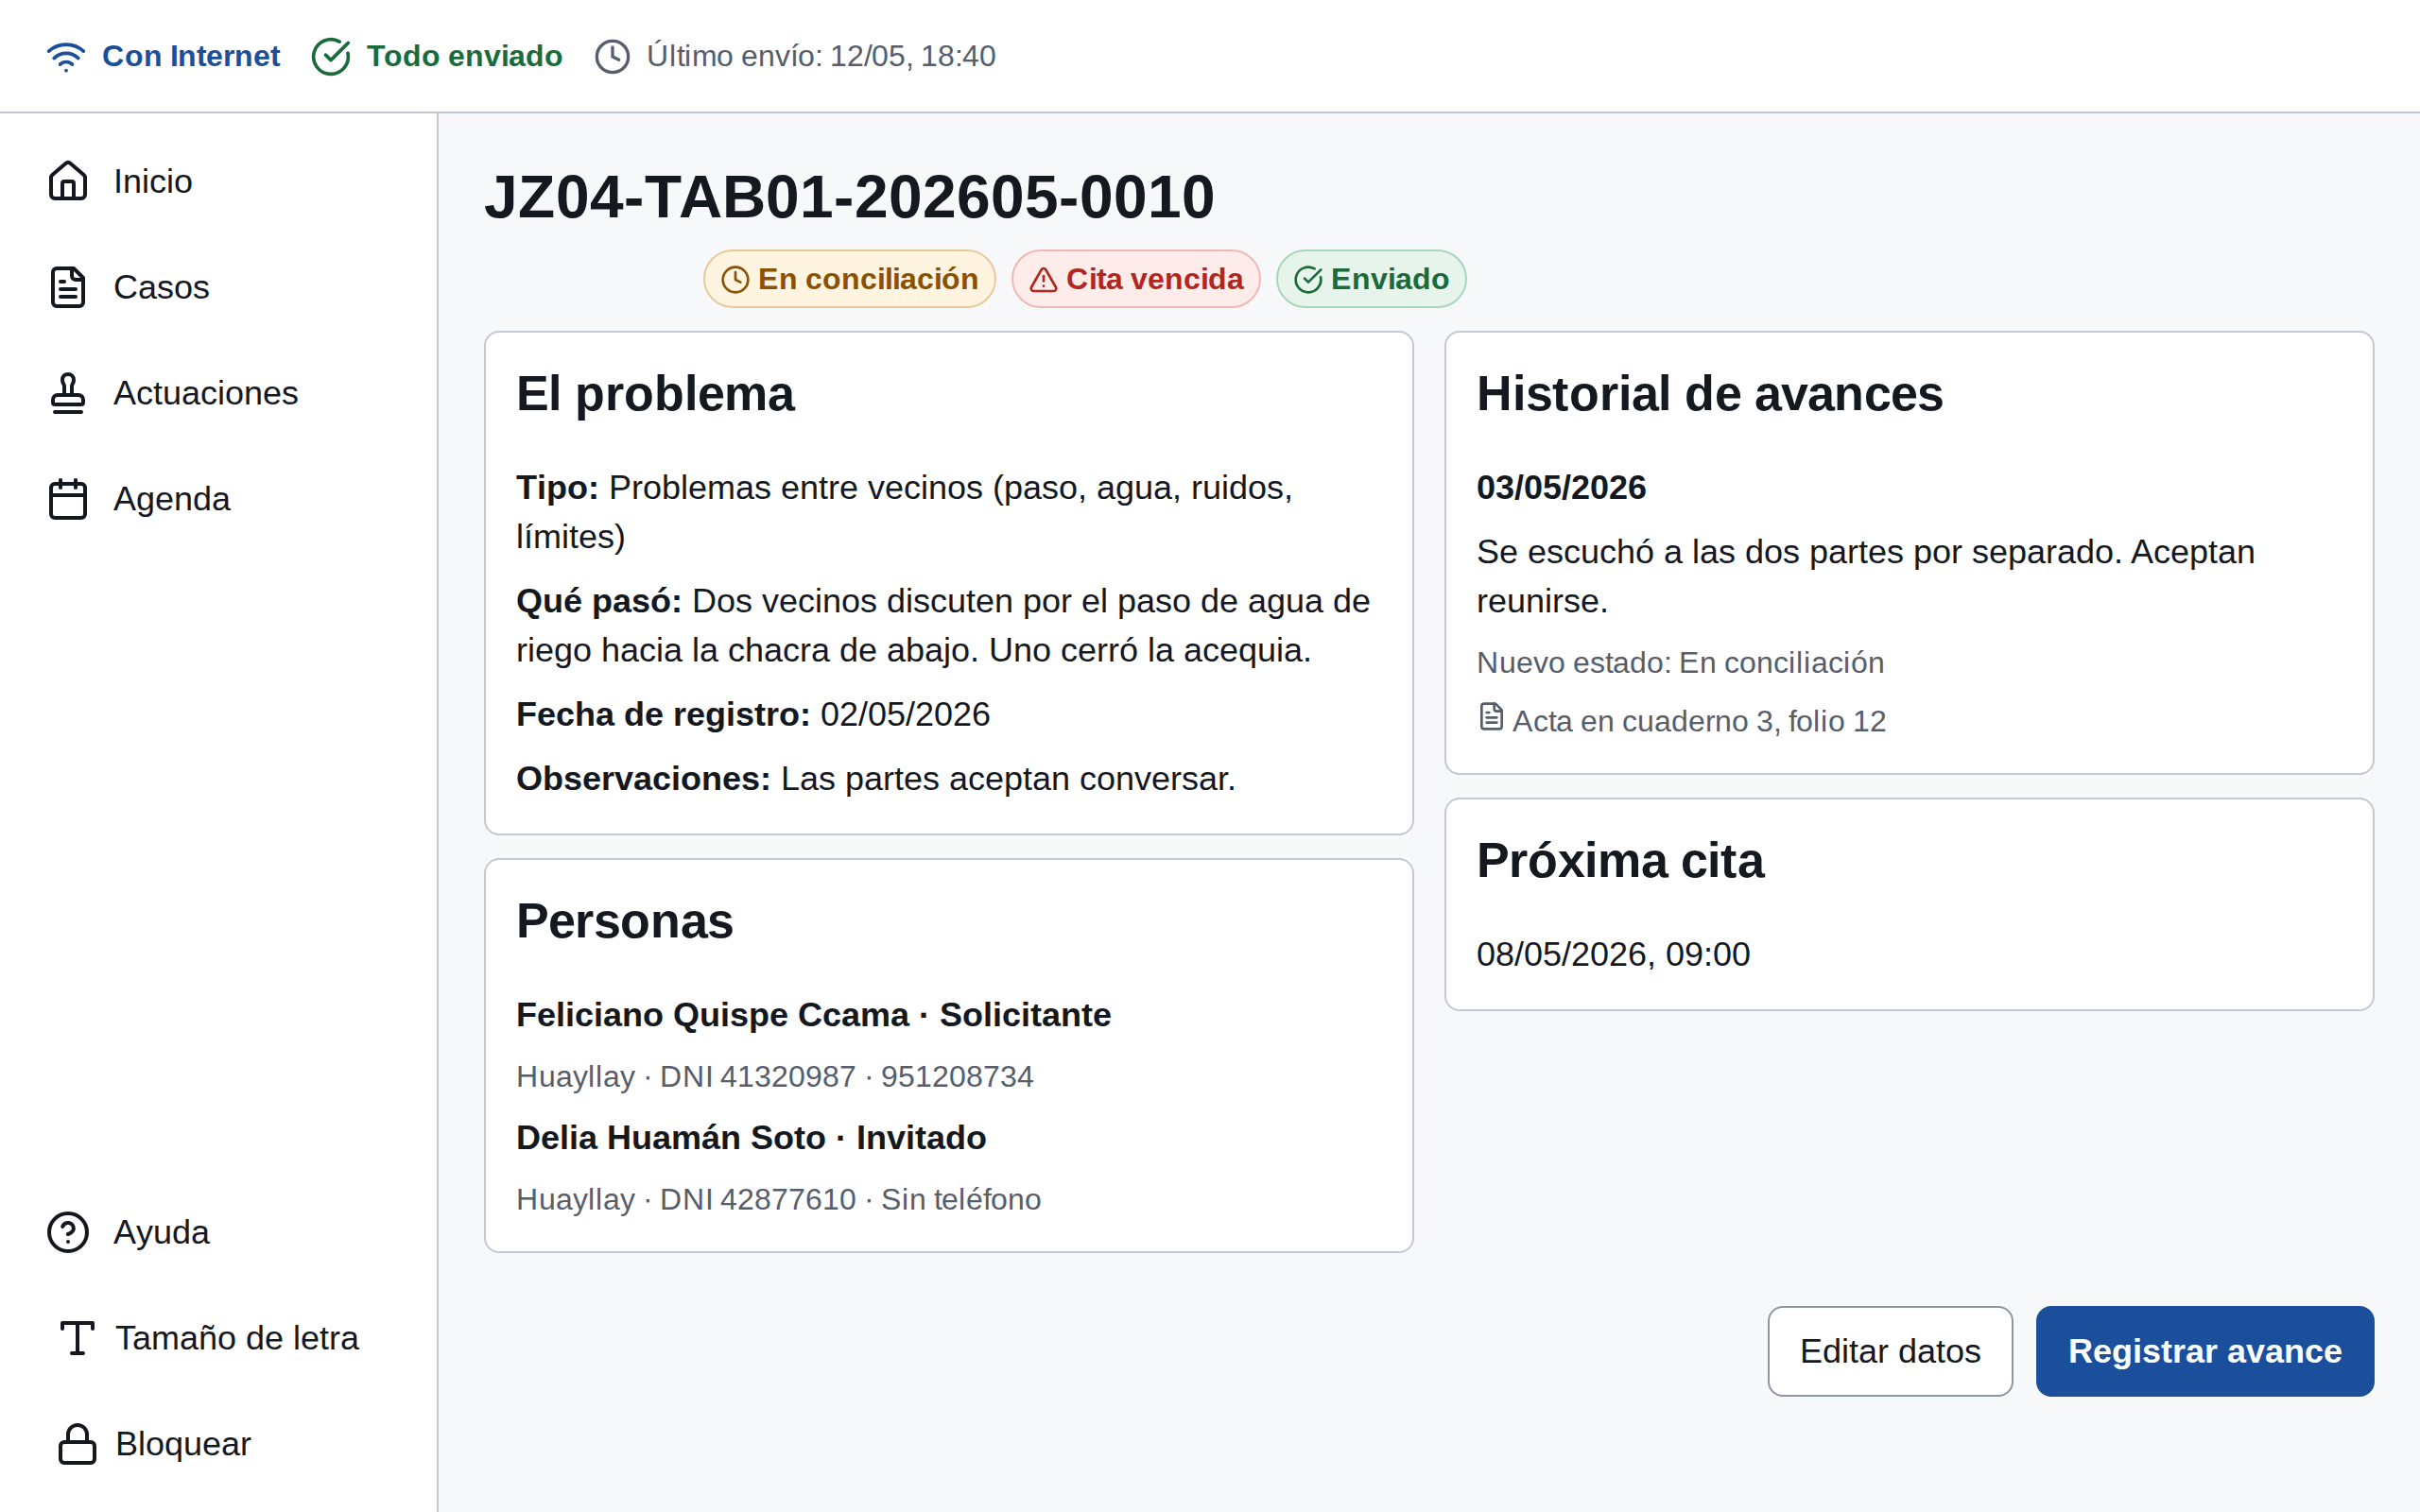
\includegraphics[width=0.82\linewidth]{capturas/FA-02_detalle-cita-vencida.png}
\caption{P-04 · 2. Caso con cita vencida. El motivo de atención se explica en texto, no solo con color}
\end{figure}
\begin{figure}[H]\centering
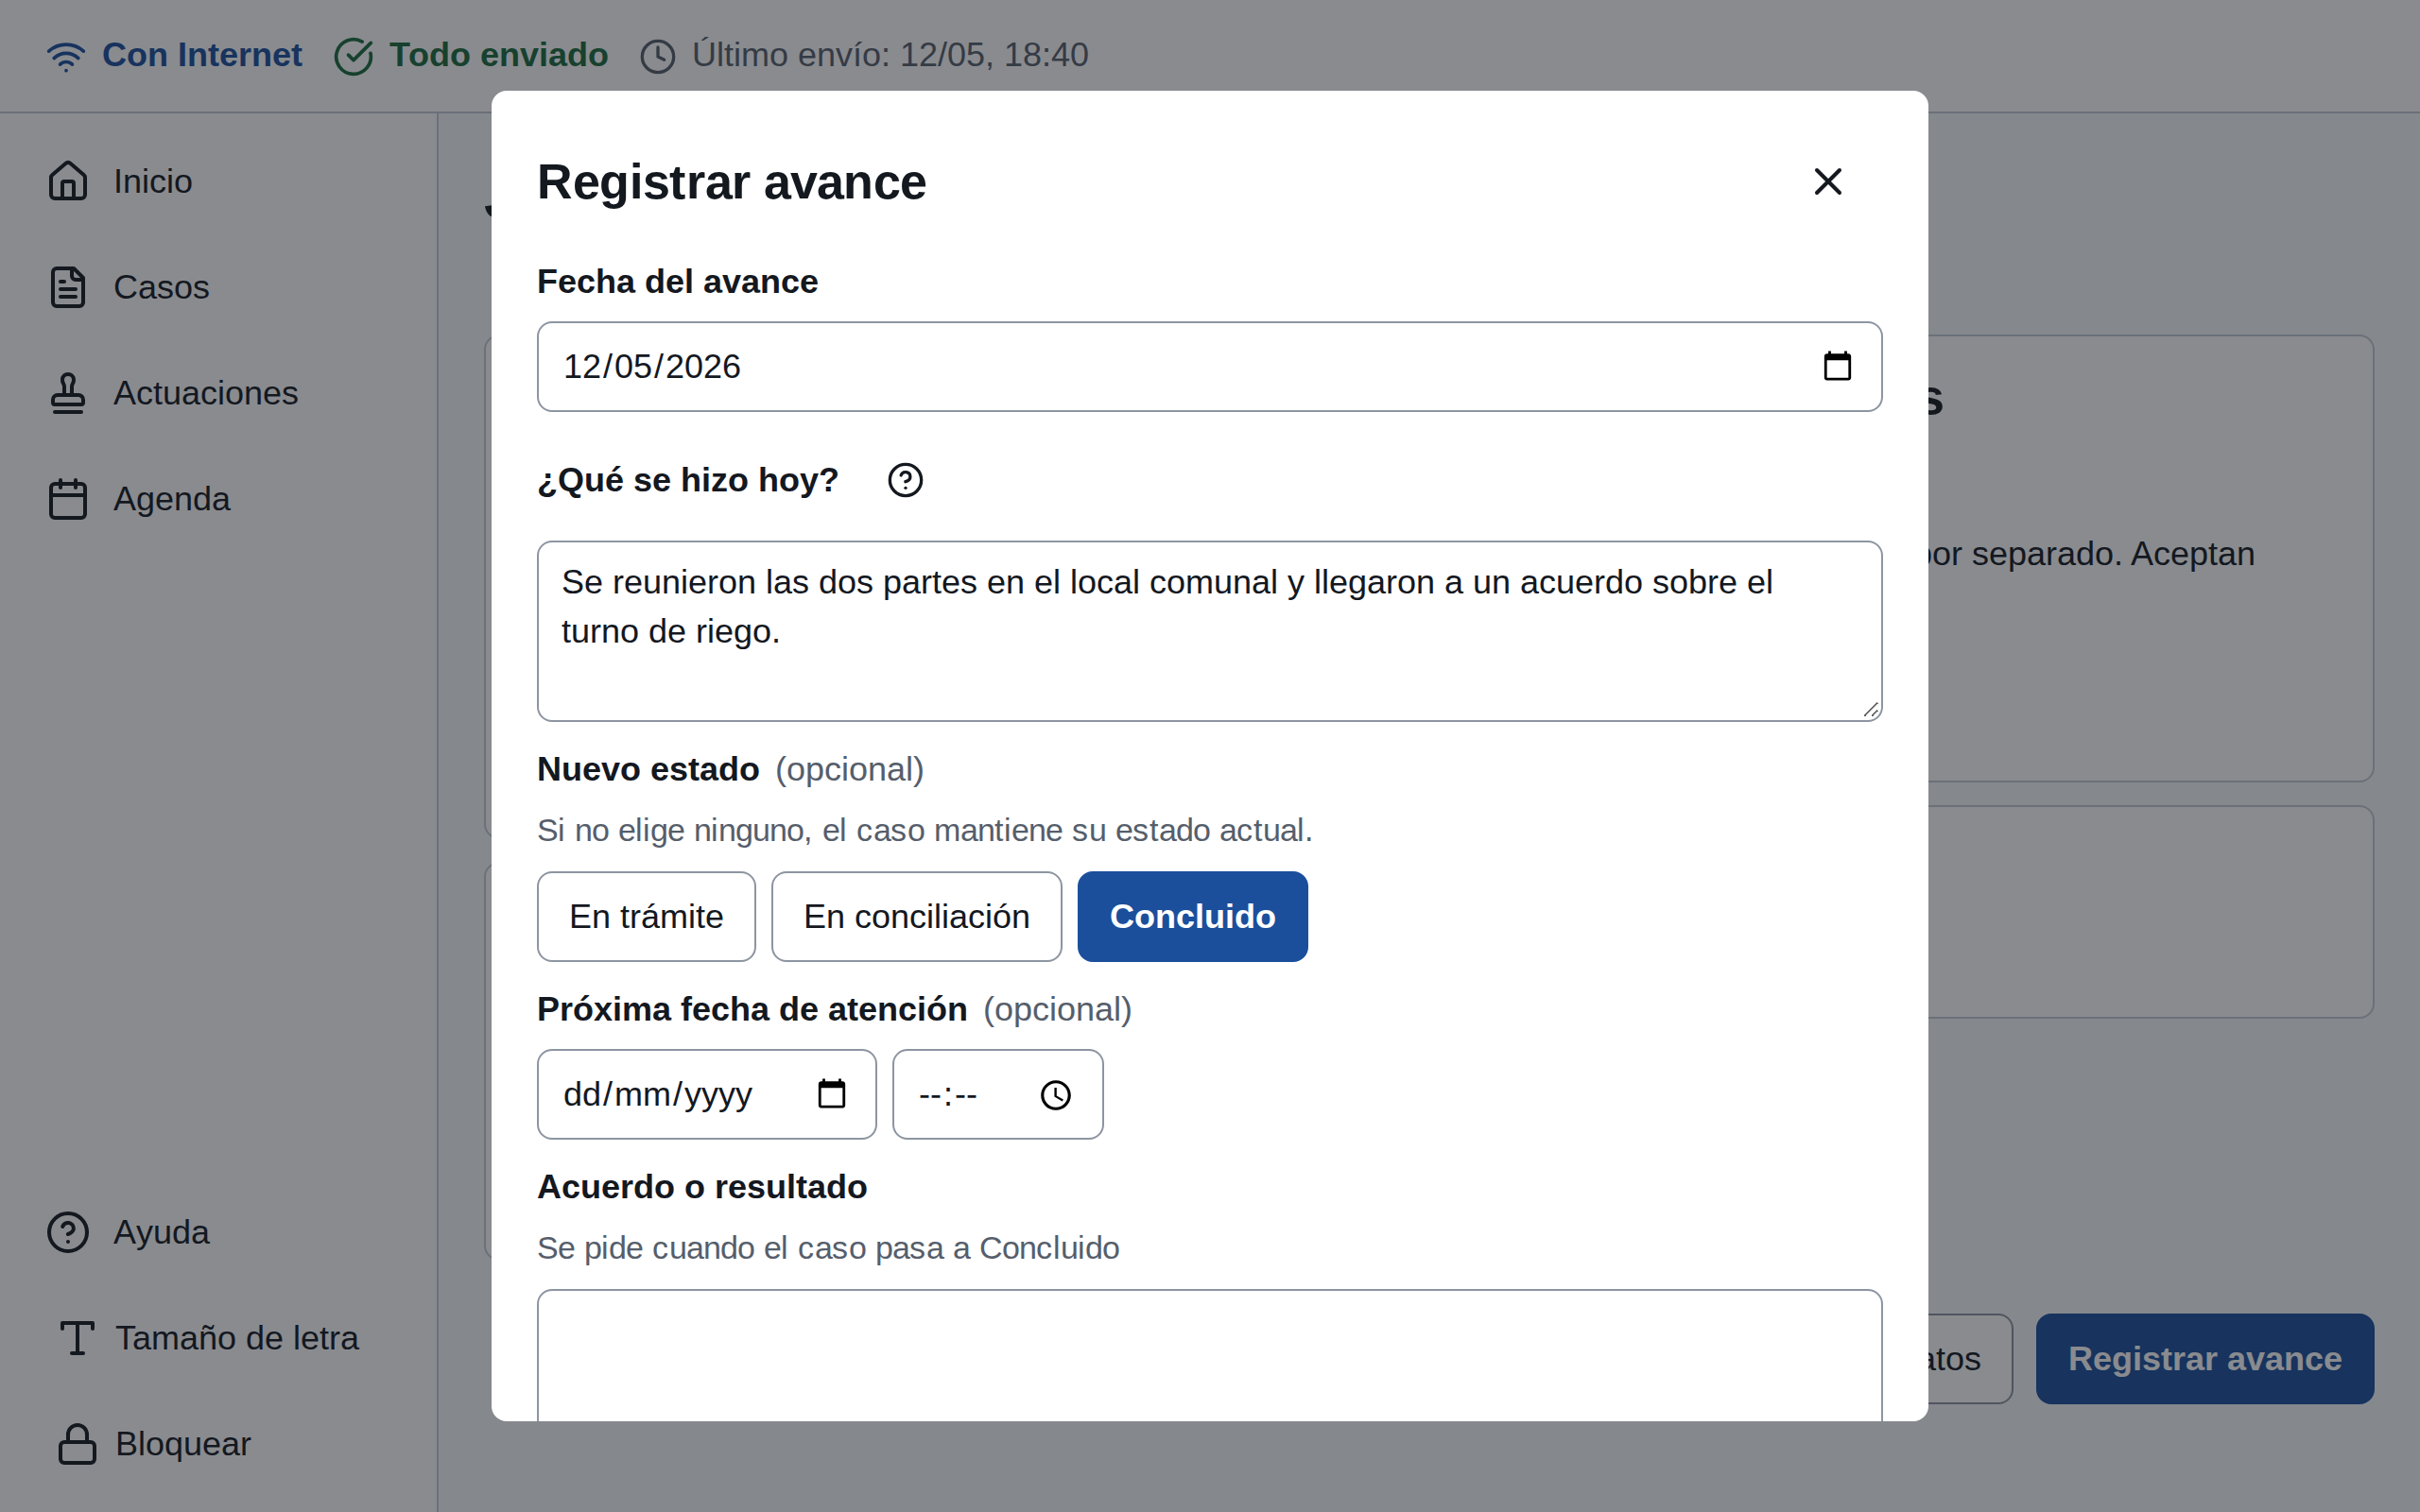
\includegraphics[width=0.82\linewidth]{capturas/FA-03_avance-condicional.png}
\caption{P-04 · 3. Al concluir se pide el acuerdo. El campo condicional aparece con su línea explicativa al pasar a Concluido}
\end{figure}
\begin{figure}[H]\centering
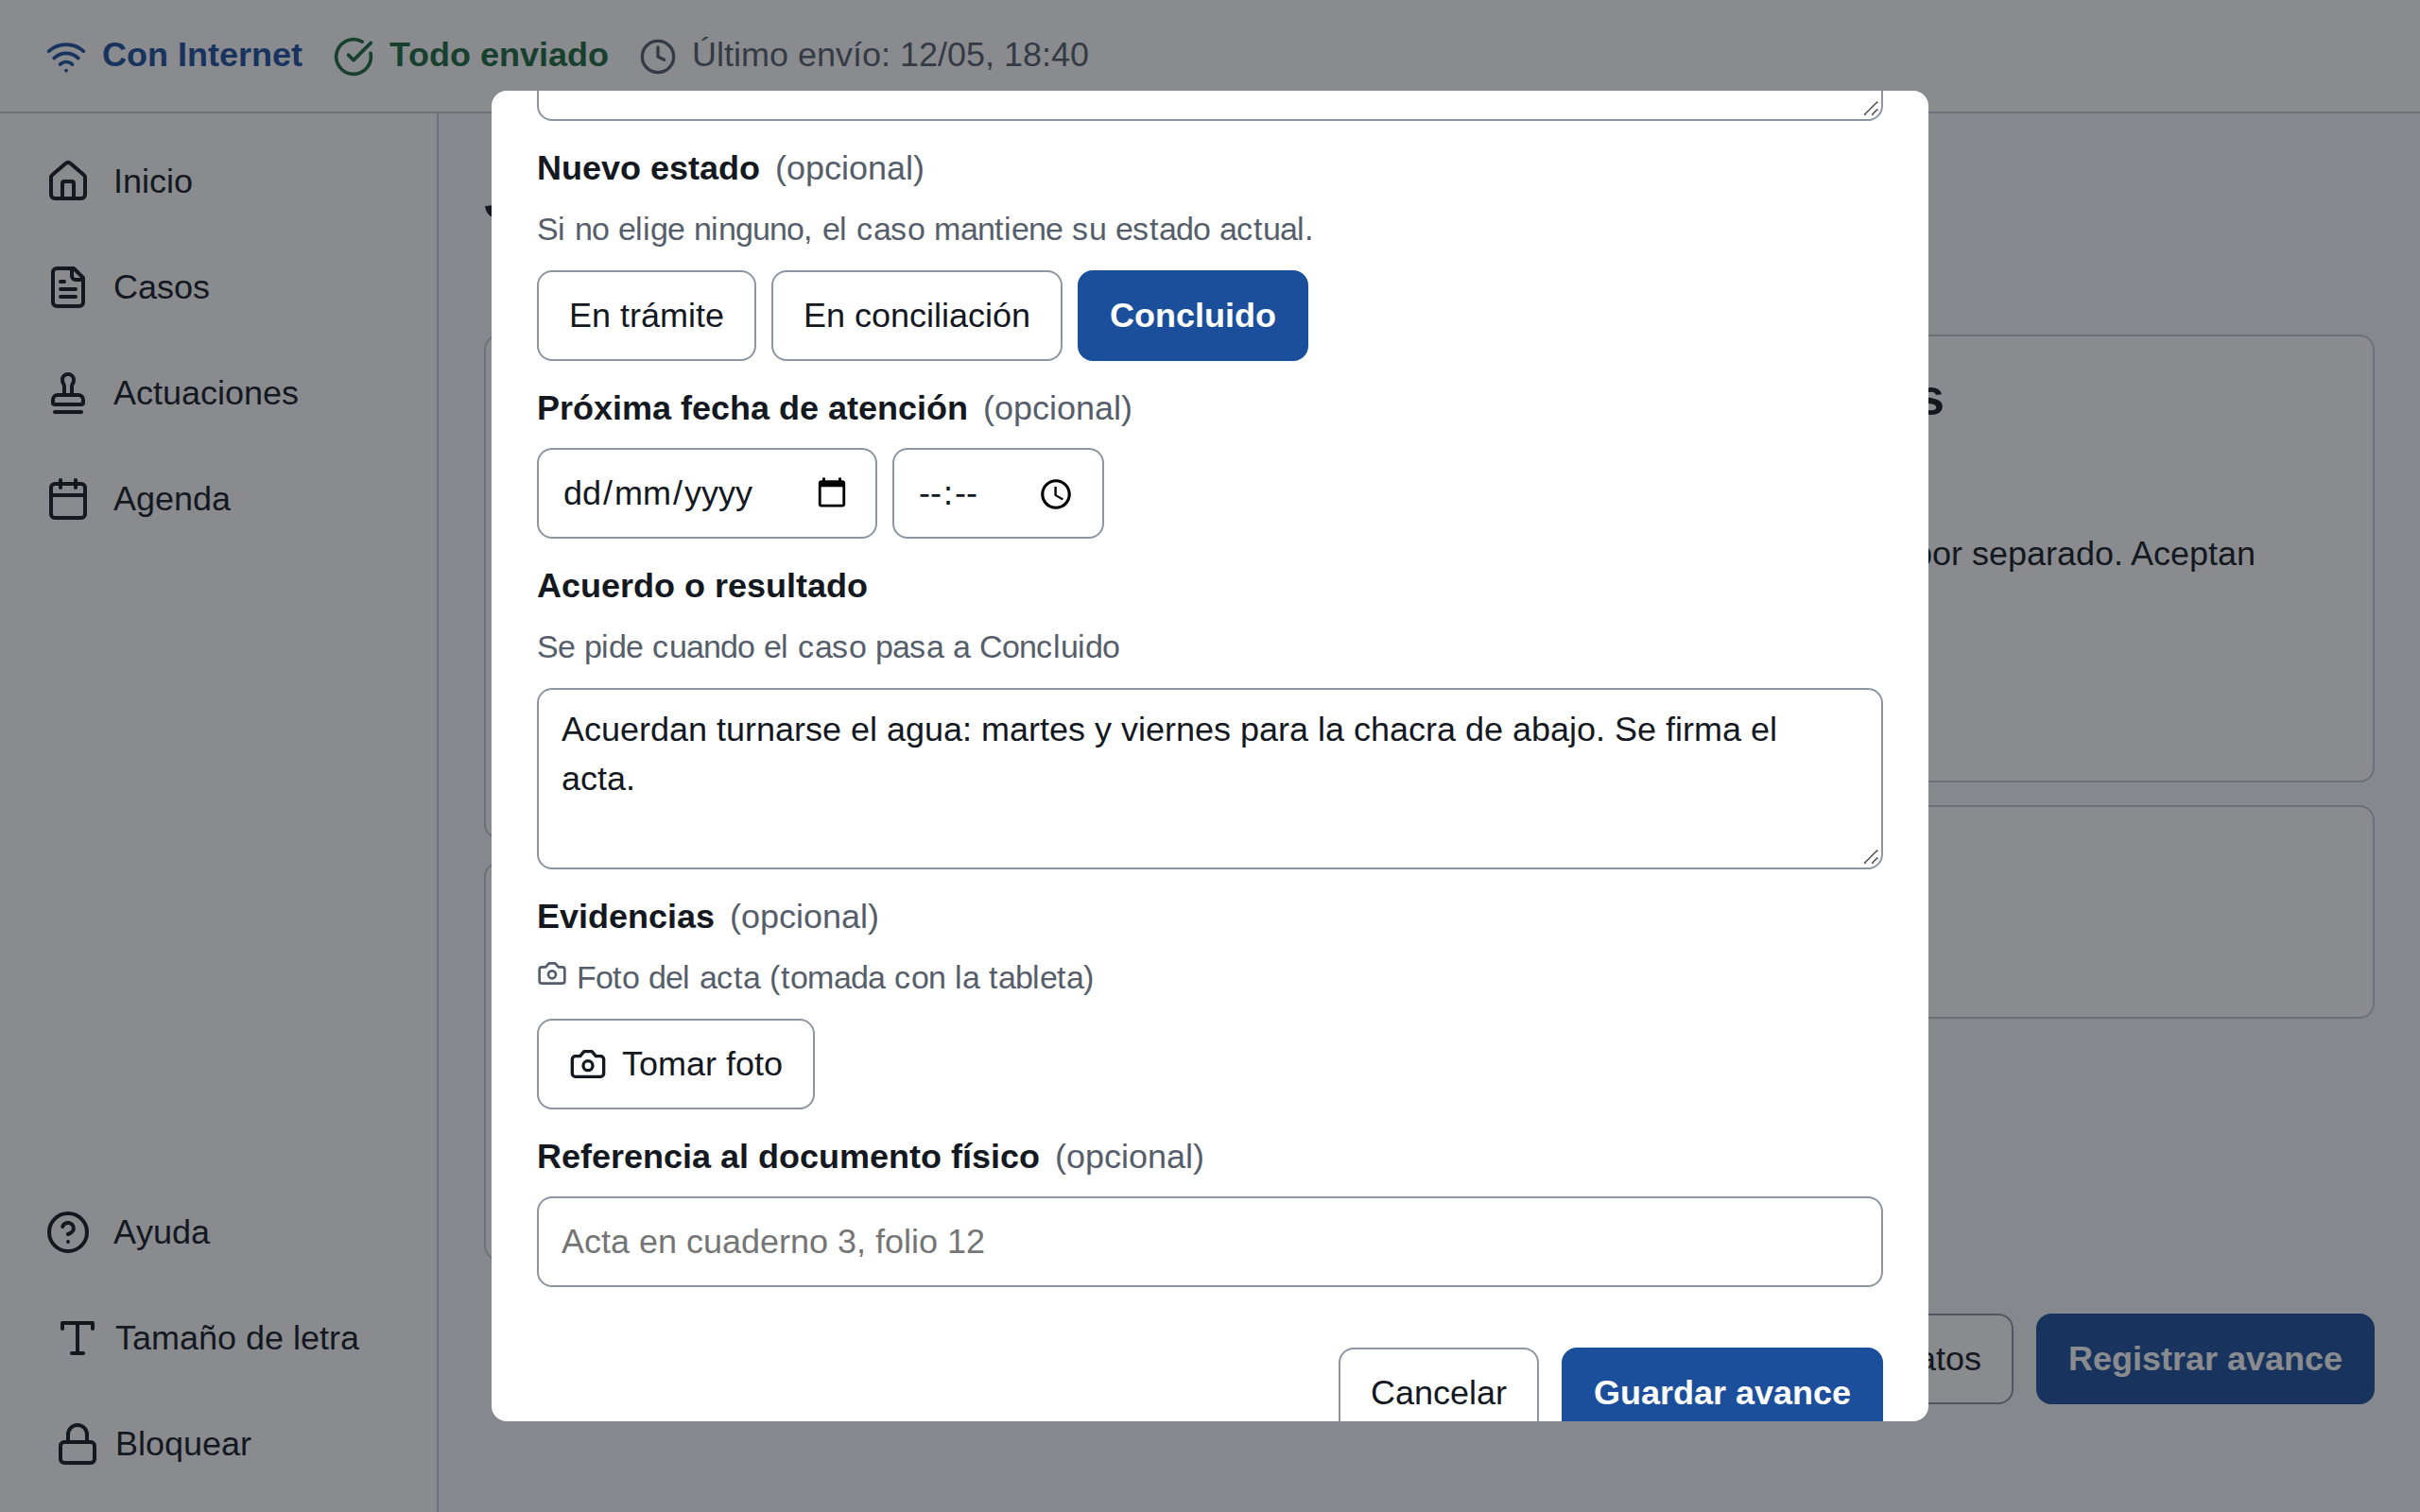
\includegraphics[width=0.82\linewidth]{capturas/FA-04_evidencia.png}
\caption{P-04 · 3. Evidencia del acta. La evidencia admite foto o referencia al cuaderno físico}
\end{figure}
\begin{figure}[H]\centering
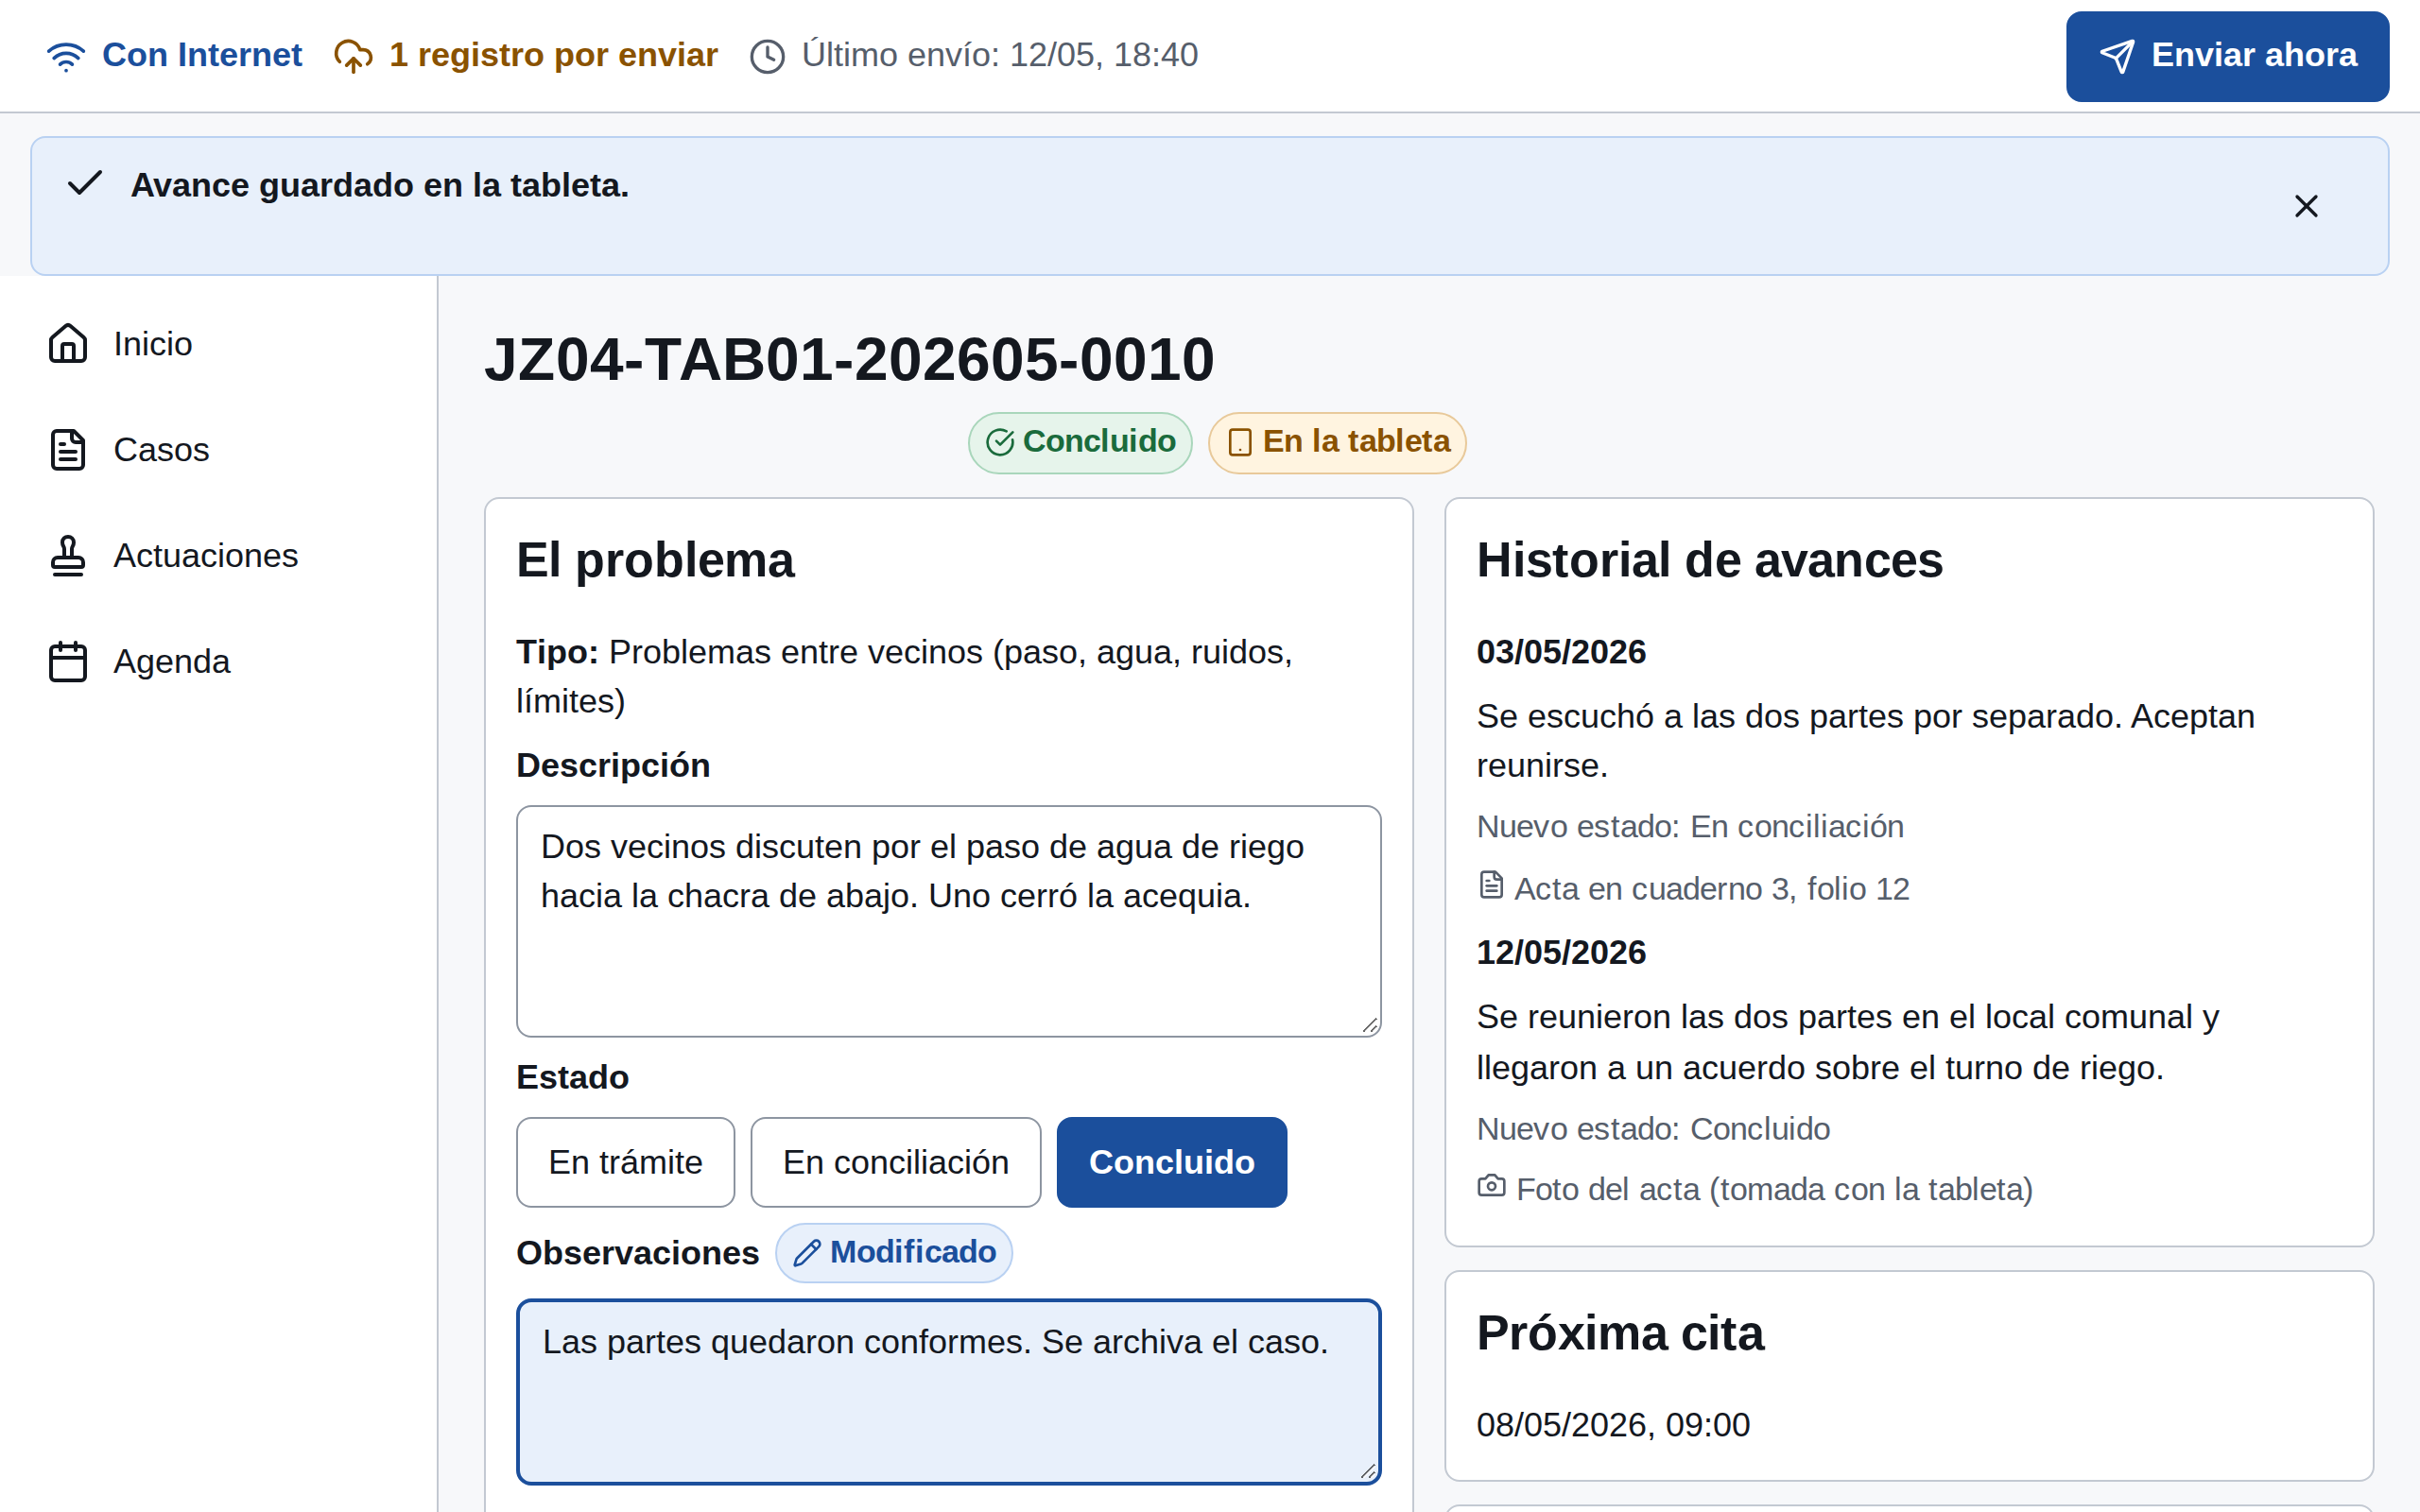
\includegraphics[width=0.82\linewidth]{capturas/FA-05_modificado.png}
\caption{P-04 · 4. Campo modificado con Deshacer. El campo cambiado se resalta y se puede deshacer antes de guardar}
\end{figure}
\begin{figure}[H]\centering
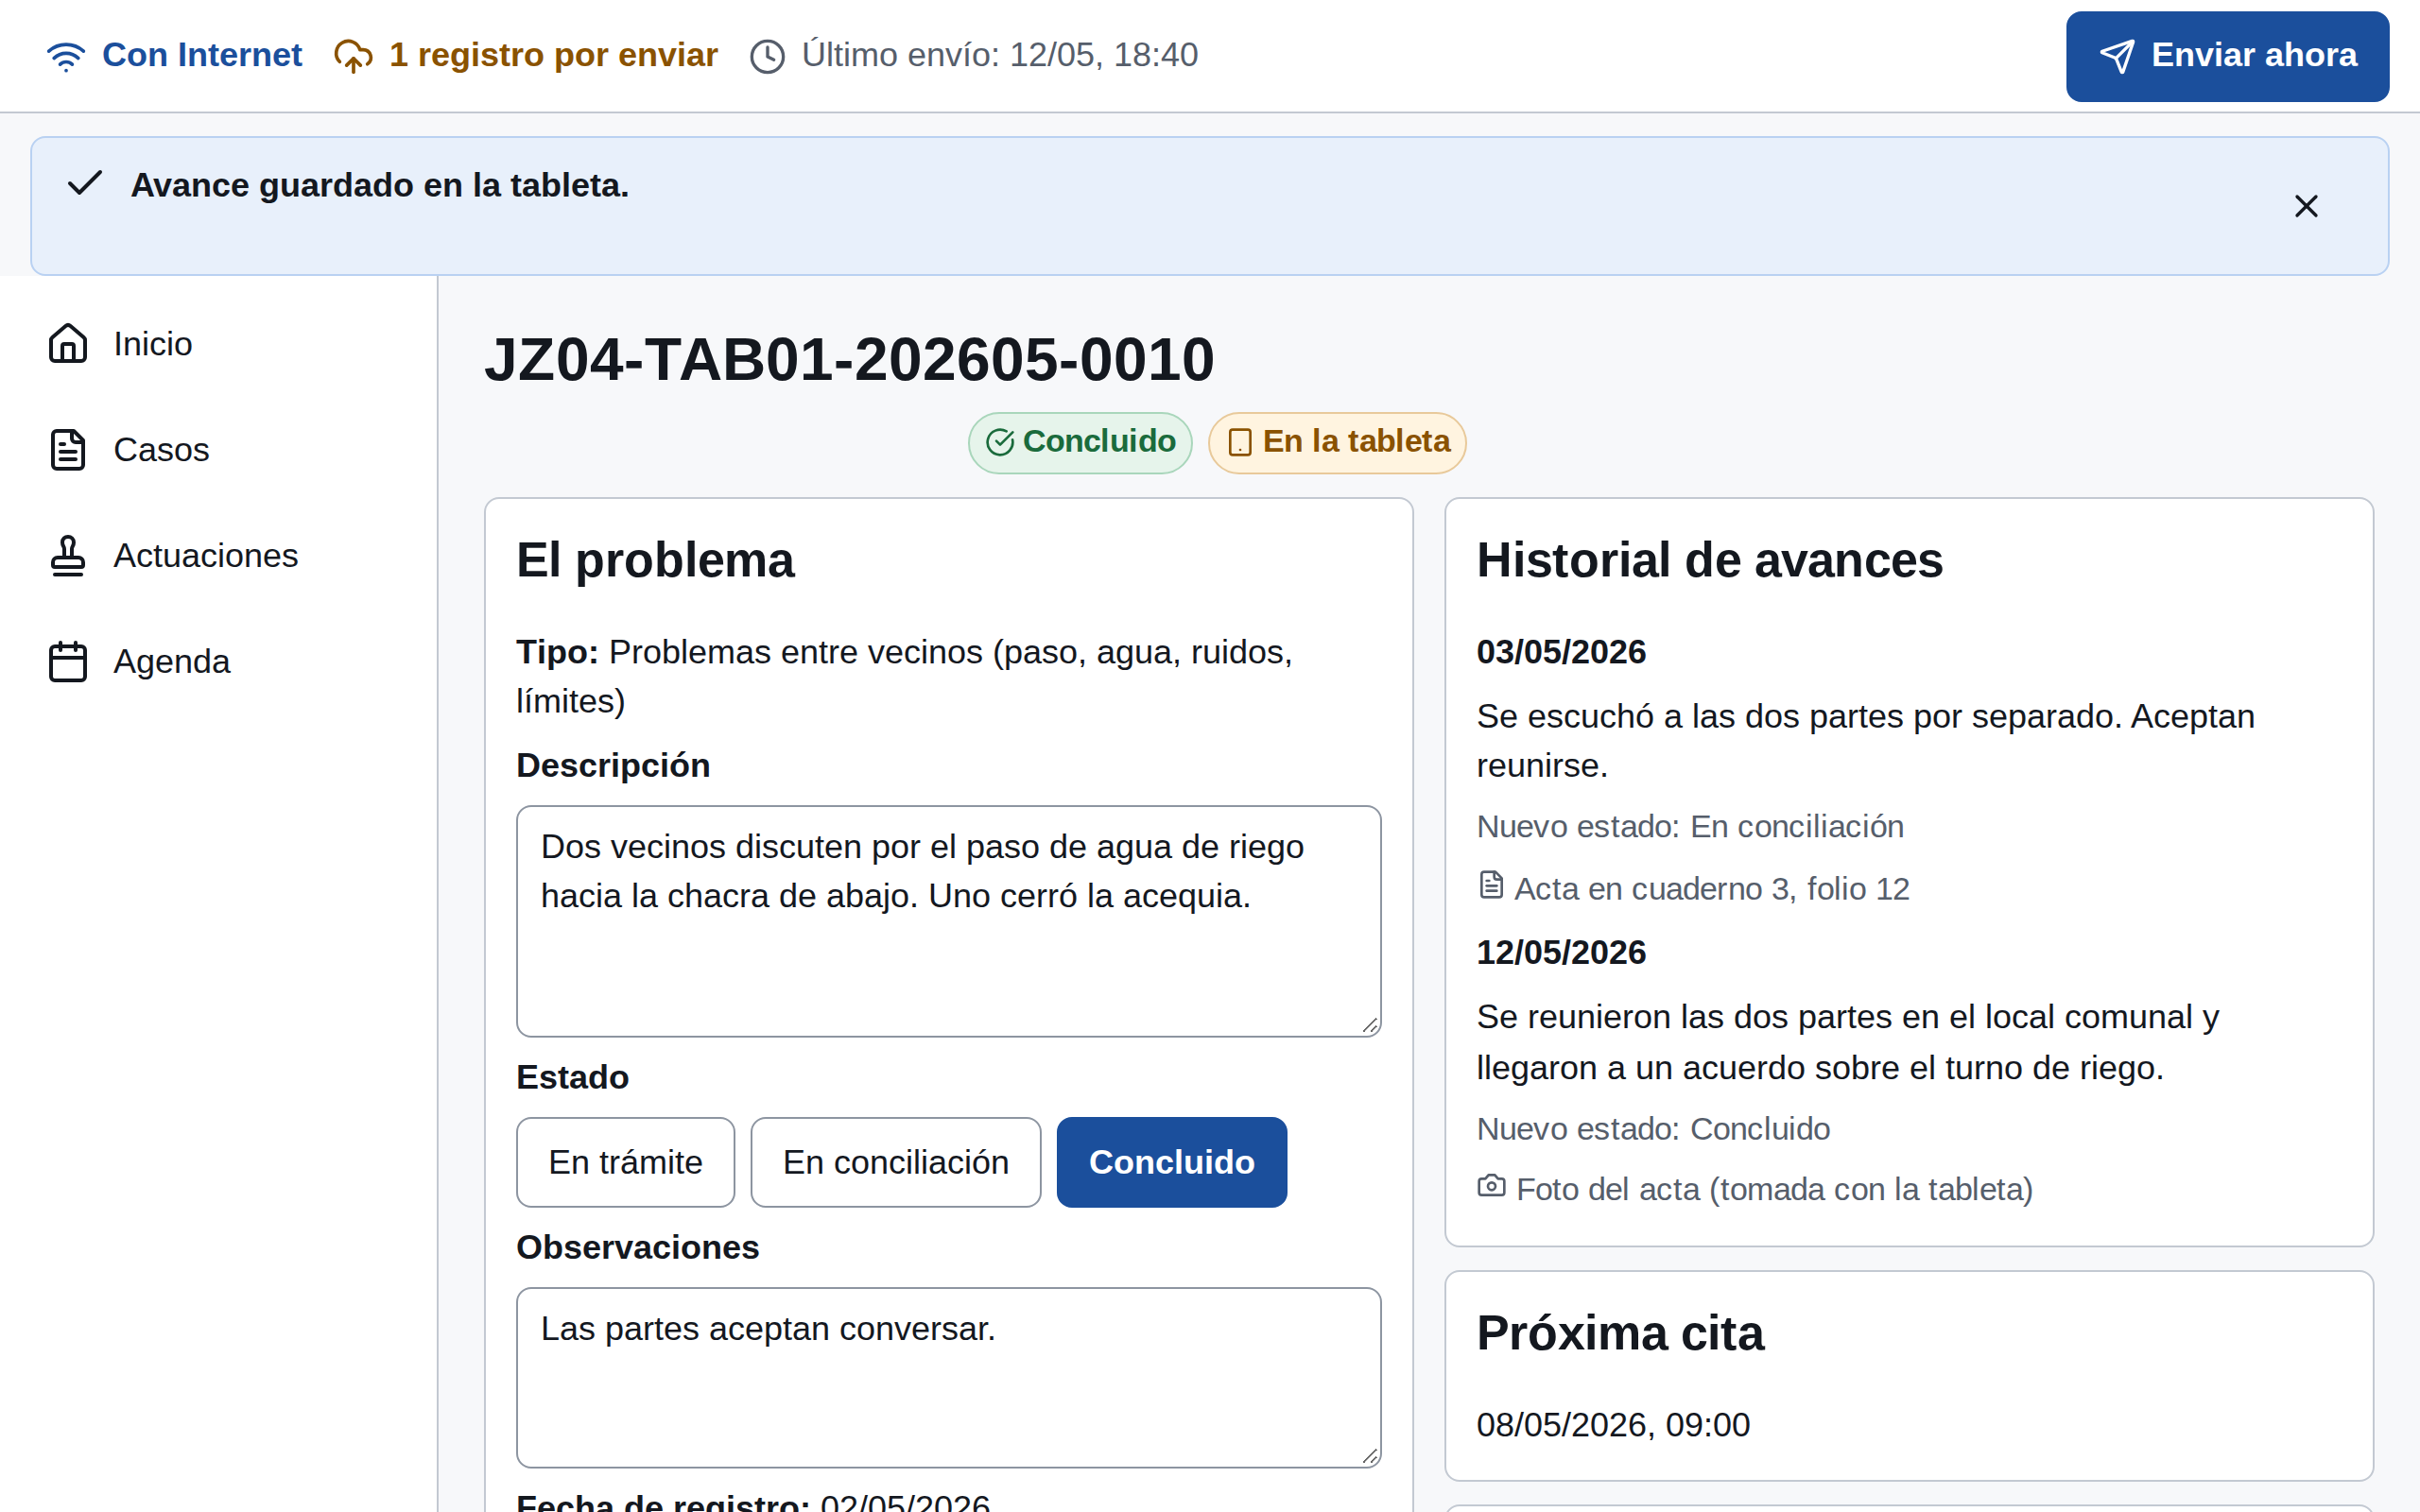
\includegraphics[width=0.82\linewidth]{capturas/FA-06_deshecho.png}
\caption{P-04 · 4. Deshecho. Deshacer devuelve el valor original sin perder el resto del trabajo}
\end{figure}
\begin{figure}[H]\centering
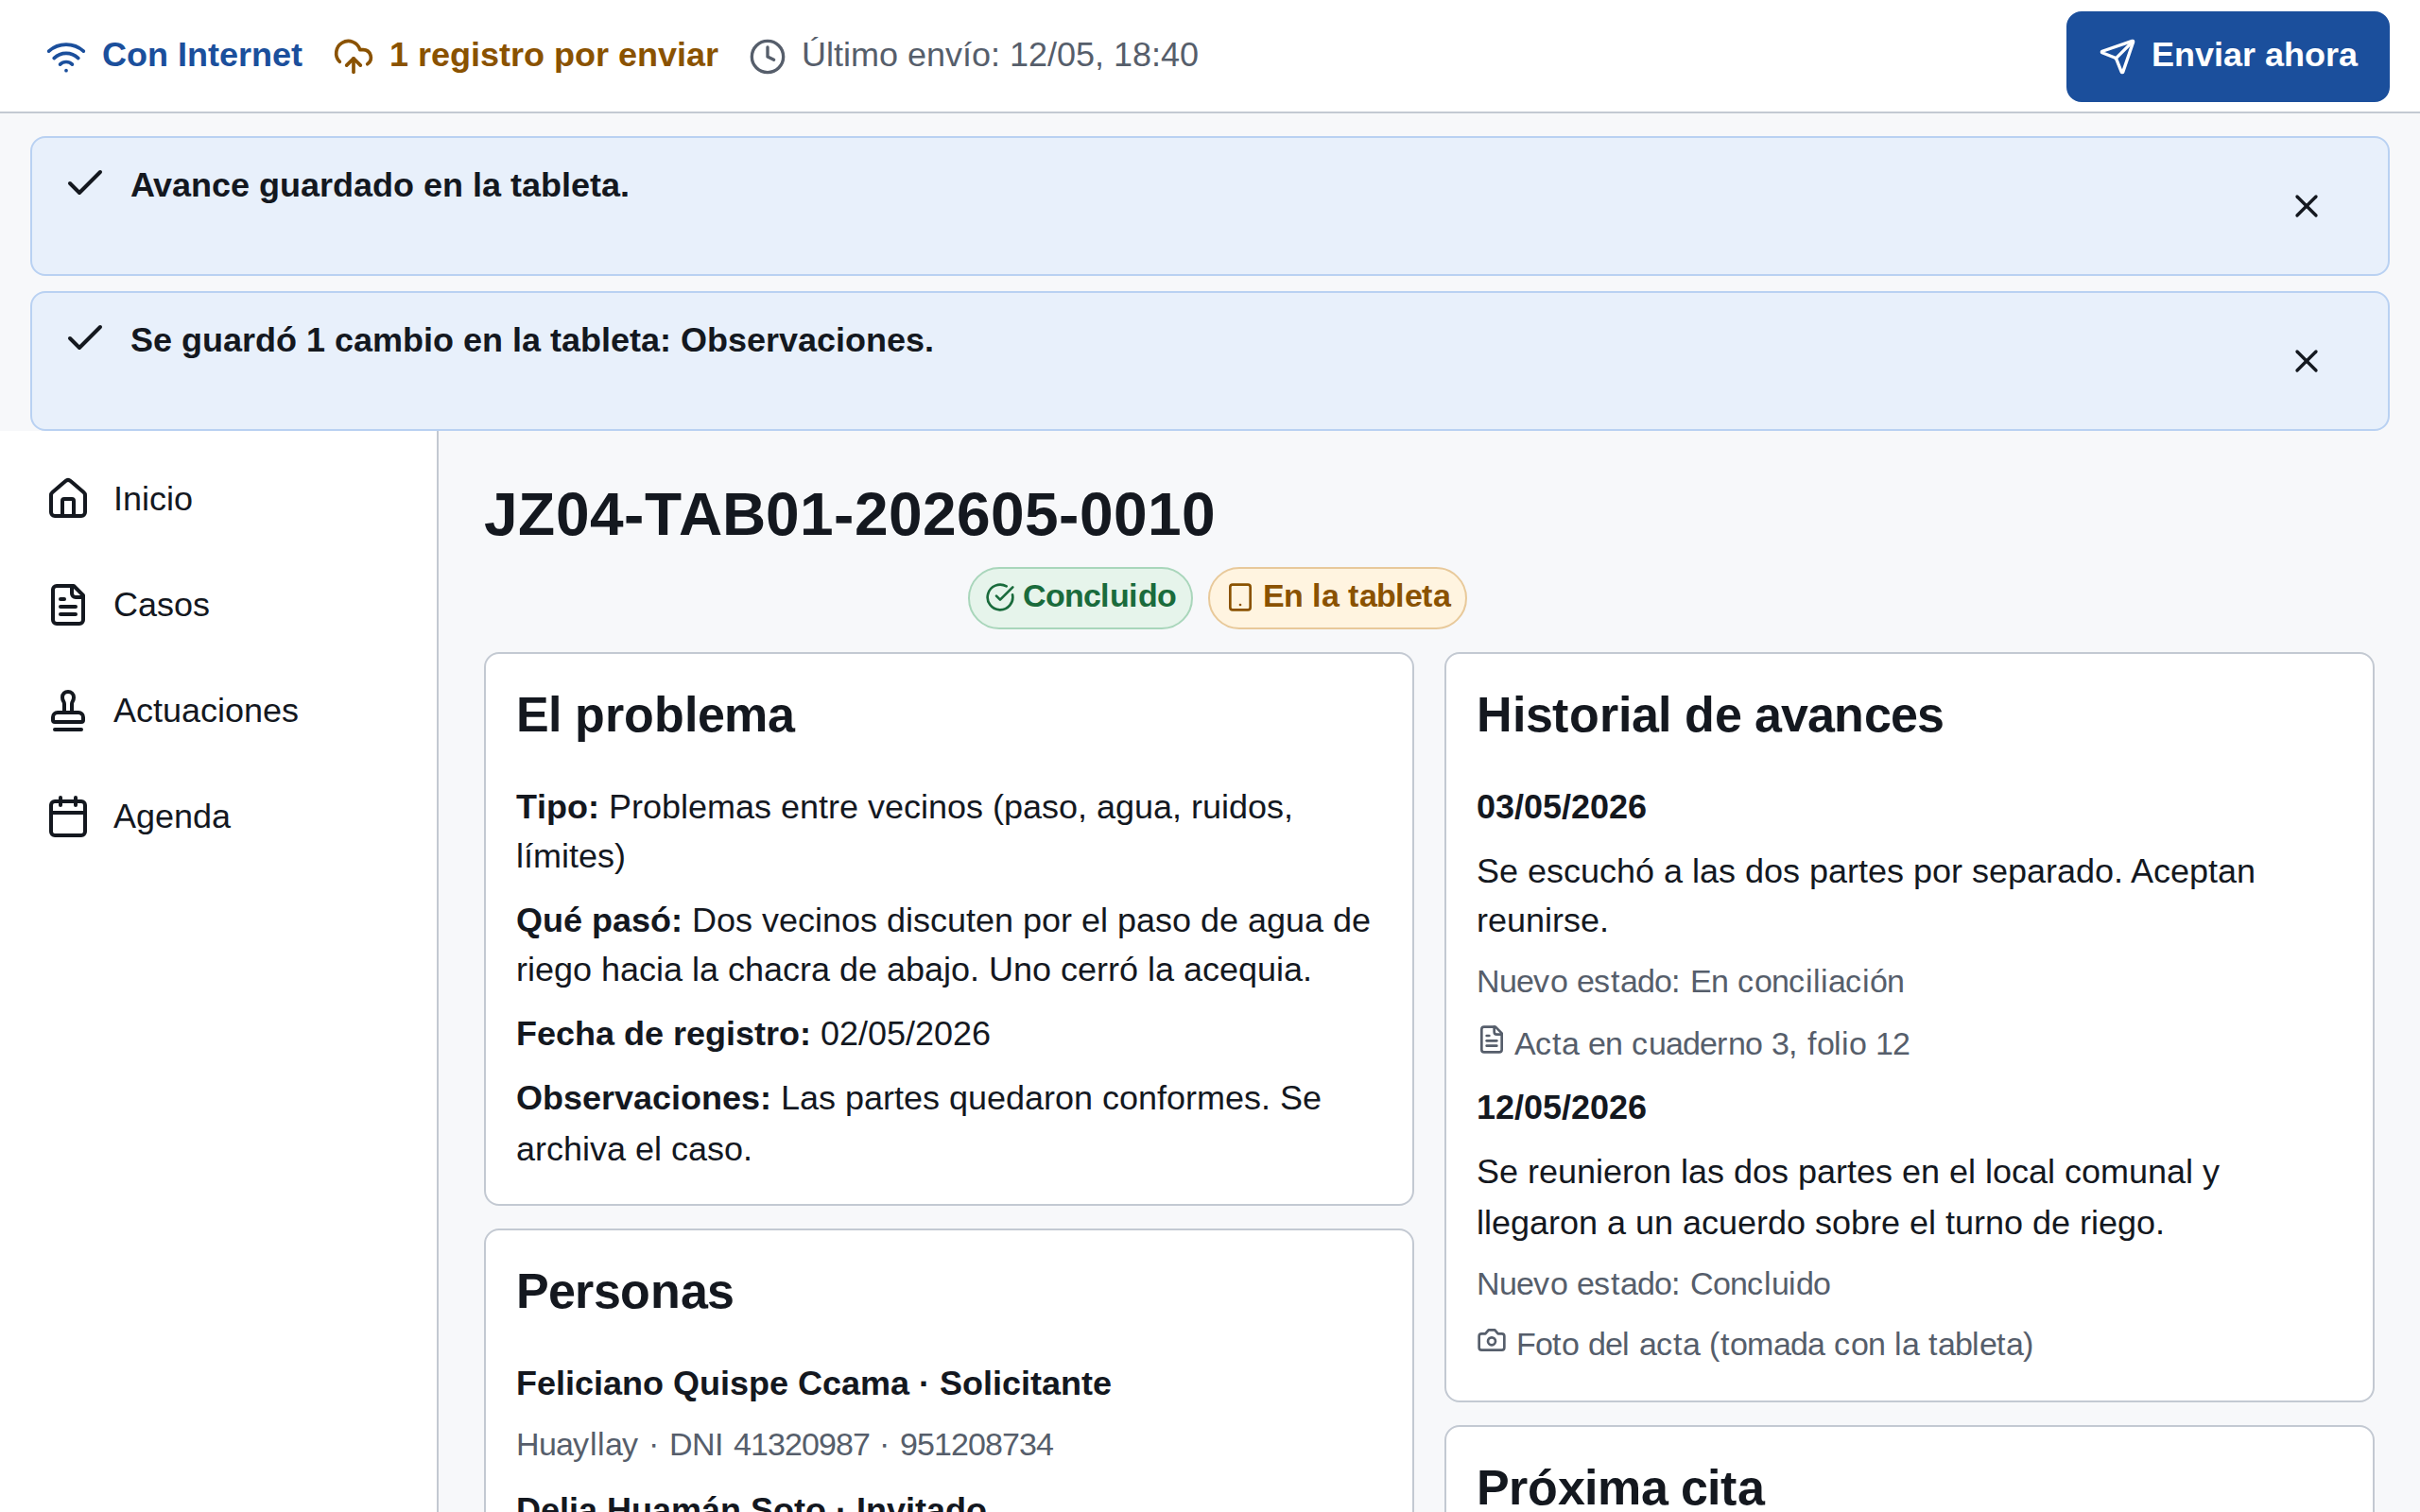
\includegraphics[width=0.82\linewidth]{capturas/FA-07_cambios-guardados.png}
\caption{P-04 · 4. Confirmación de cambios. La confirmación dice cuántos cambios se guardaron y en qué campos}
\end{figure}
\subsection{Flujo complementario B · Consultar y editar desde la computadora}
\begin{figure}[H]\centering
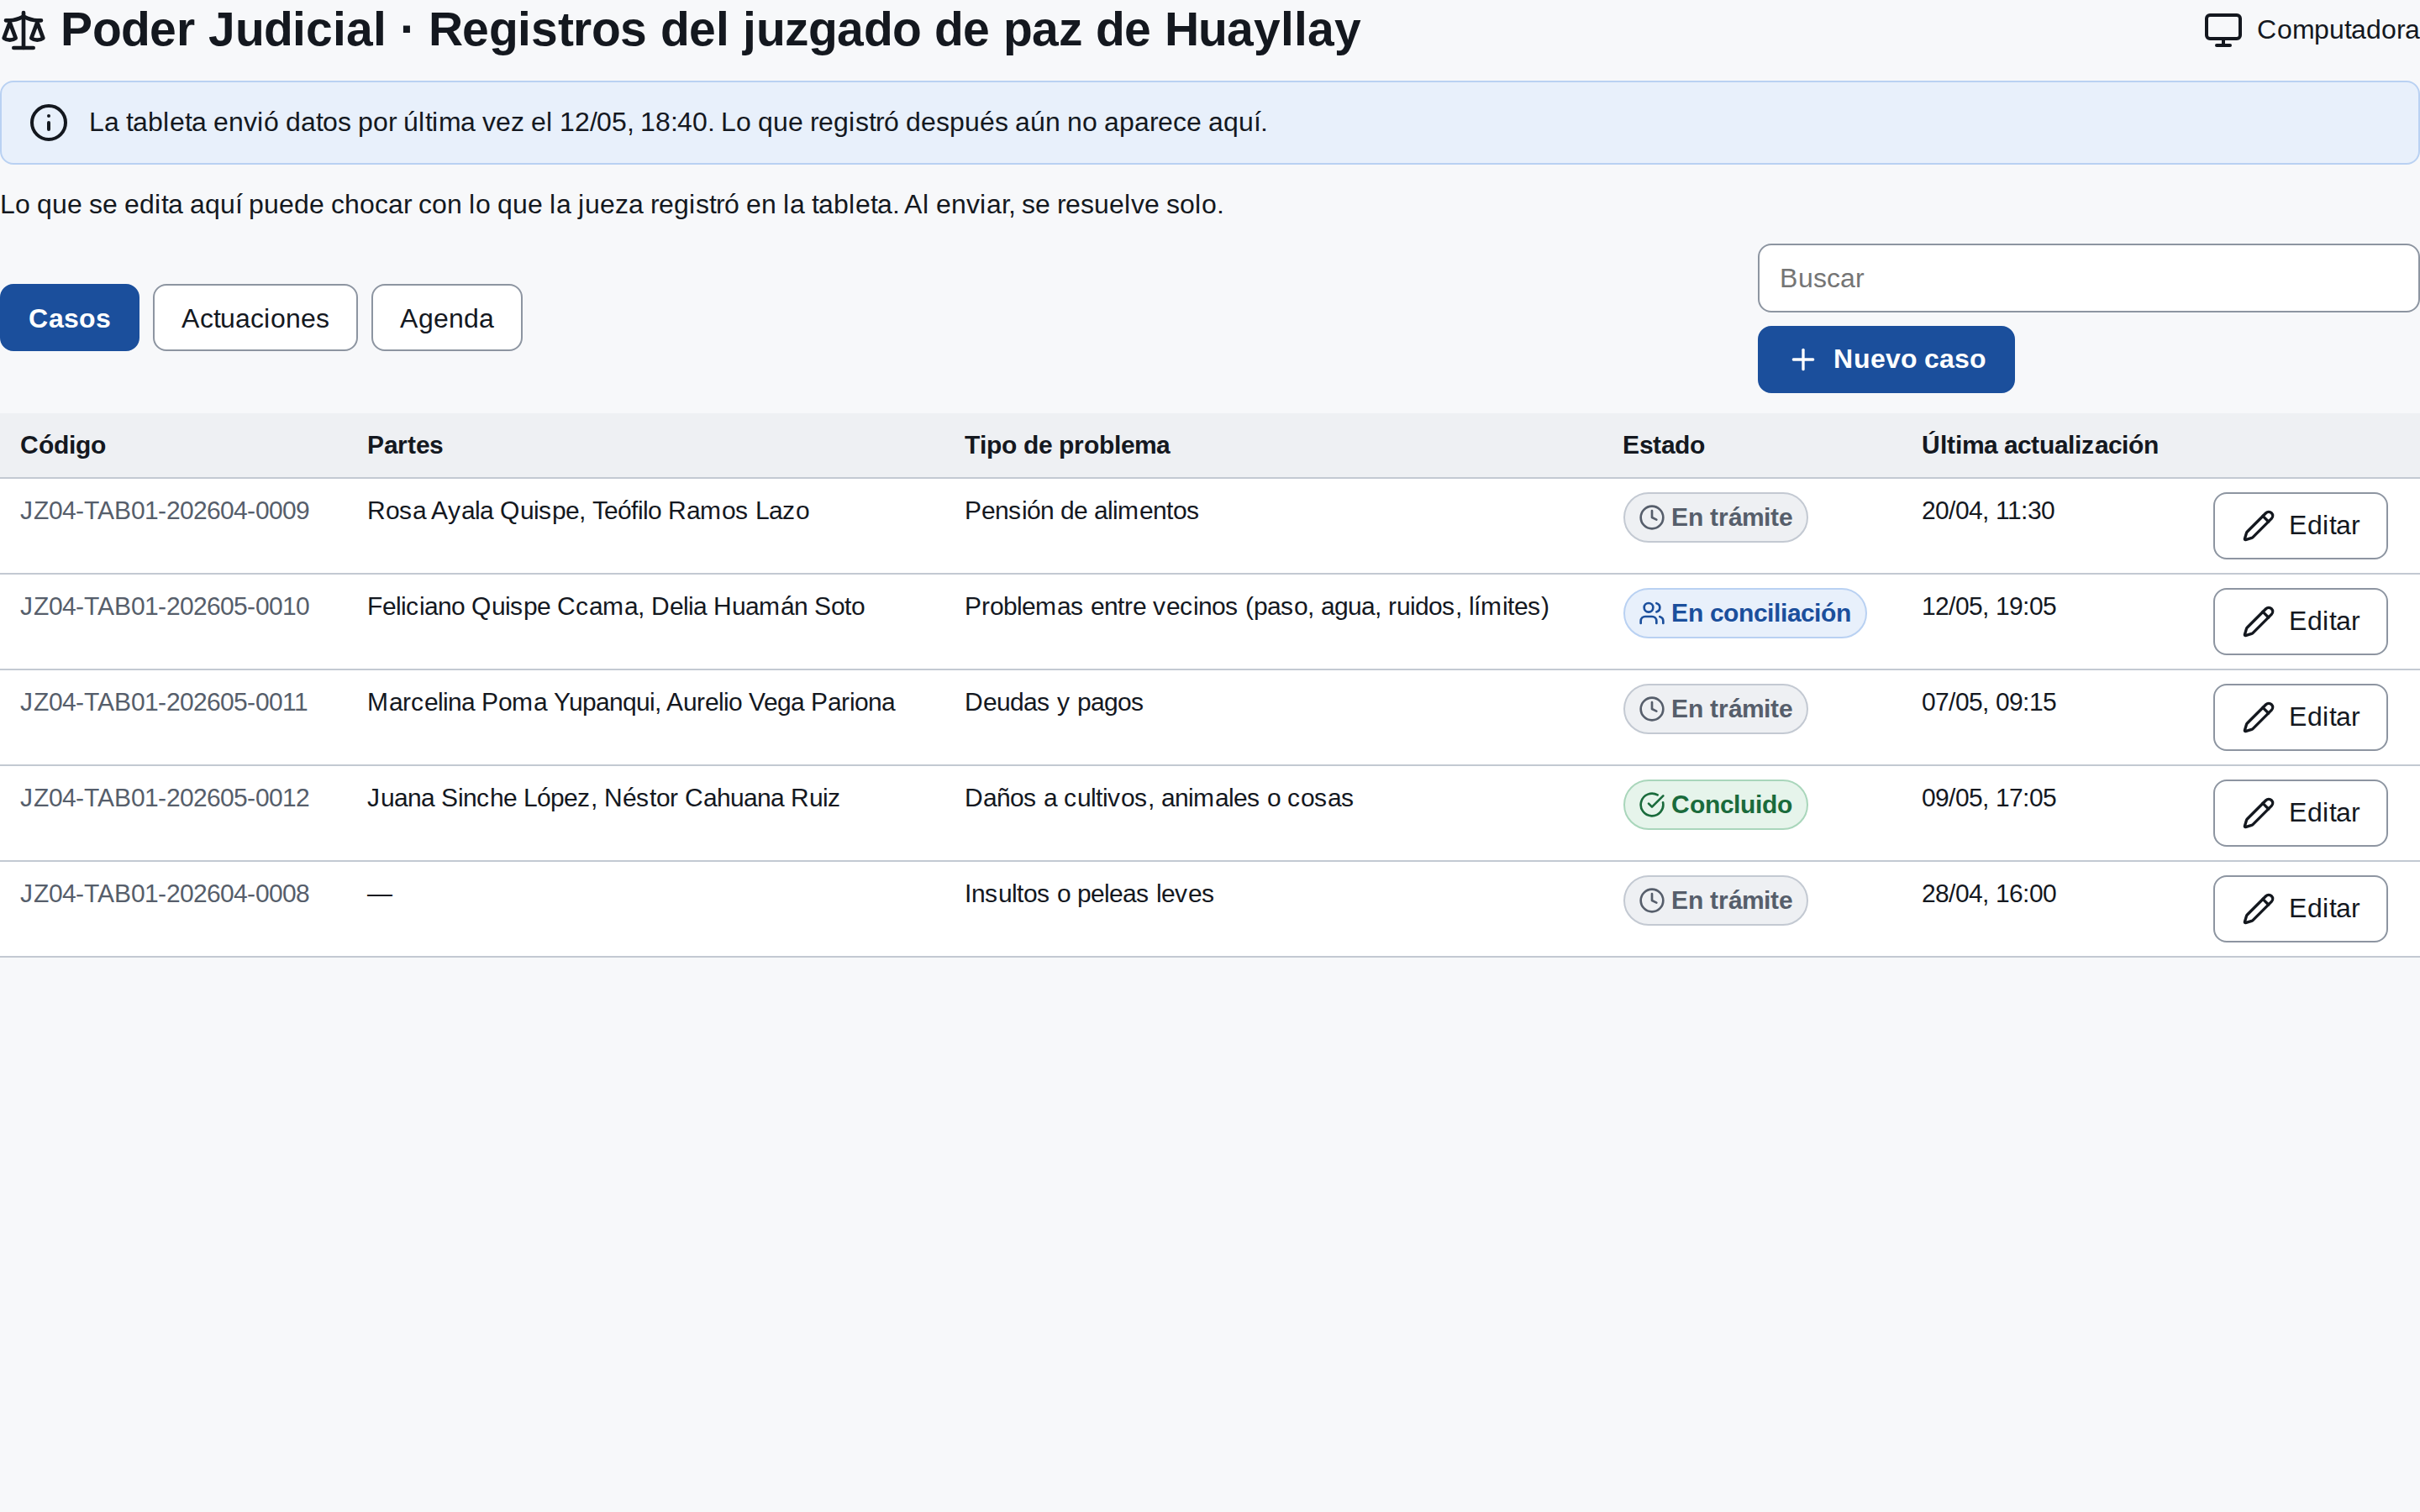
\includegraphics[width=0.82\linewidth]{capturas/FB-01_pc-casos.png}
\caption{P-10 · 1. Datos que ya llegaron. Aviso del último envío de la tableta, sin afirmar cuántos registros quedan pendientes}
\end{figure}
\begin{figure}[H]\centering
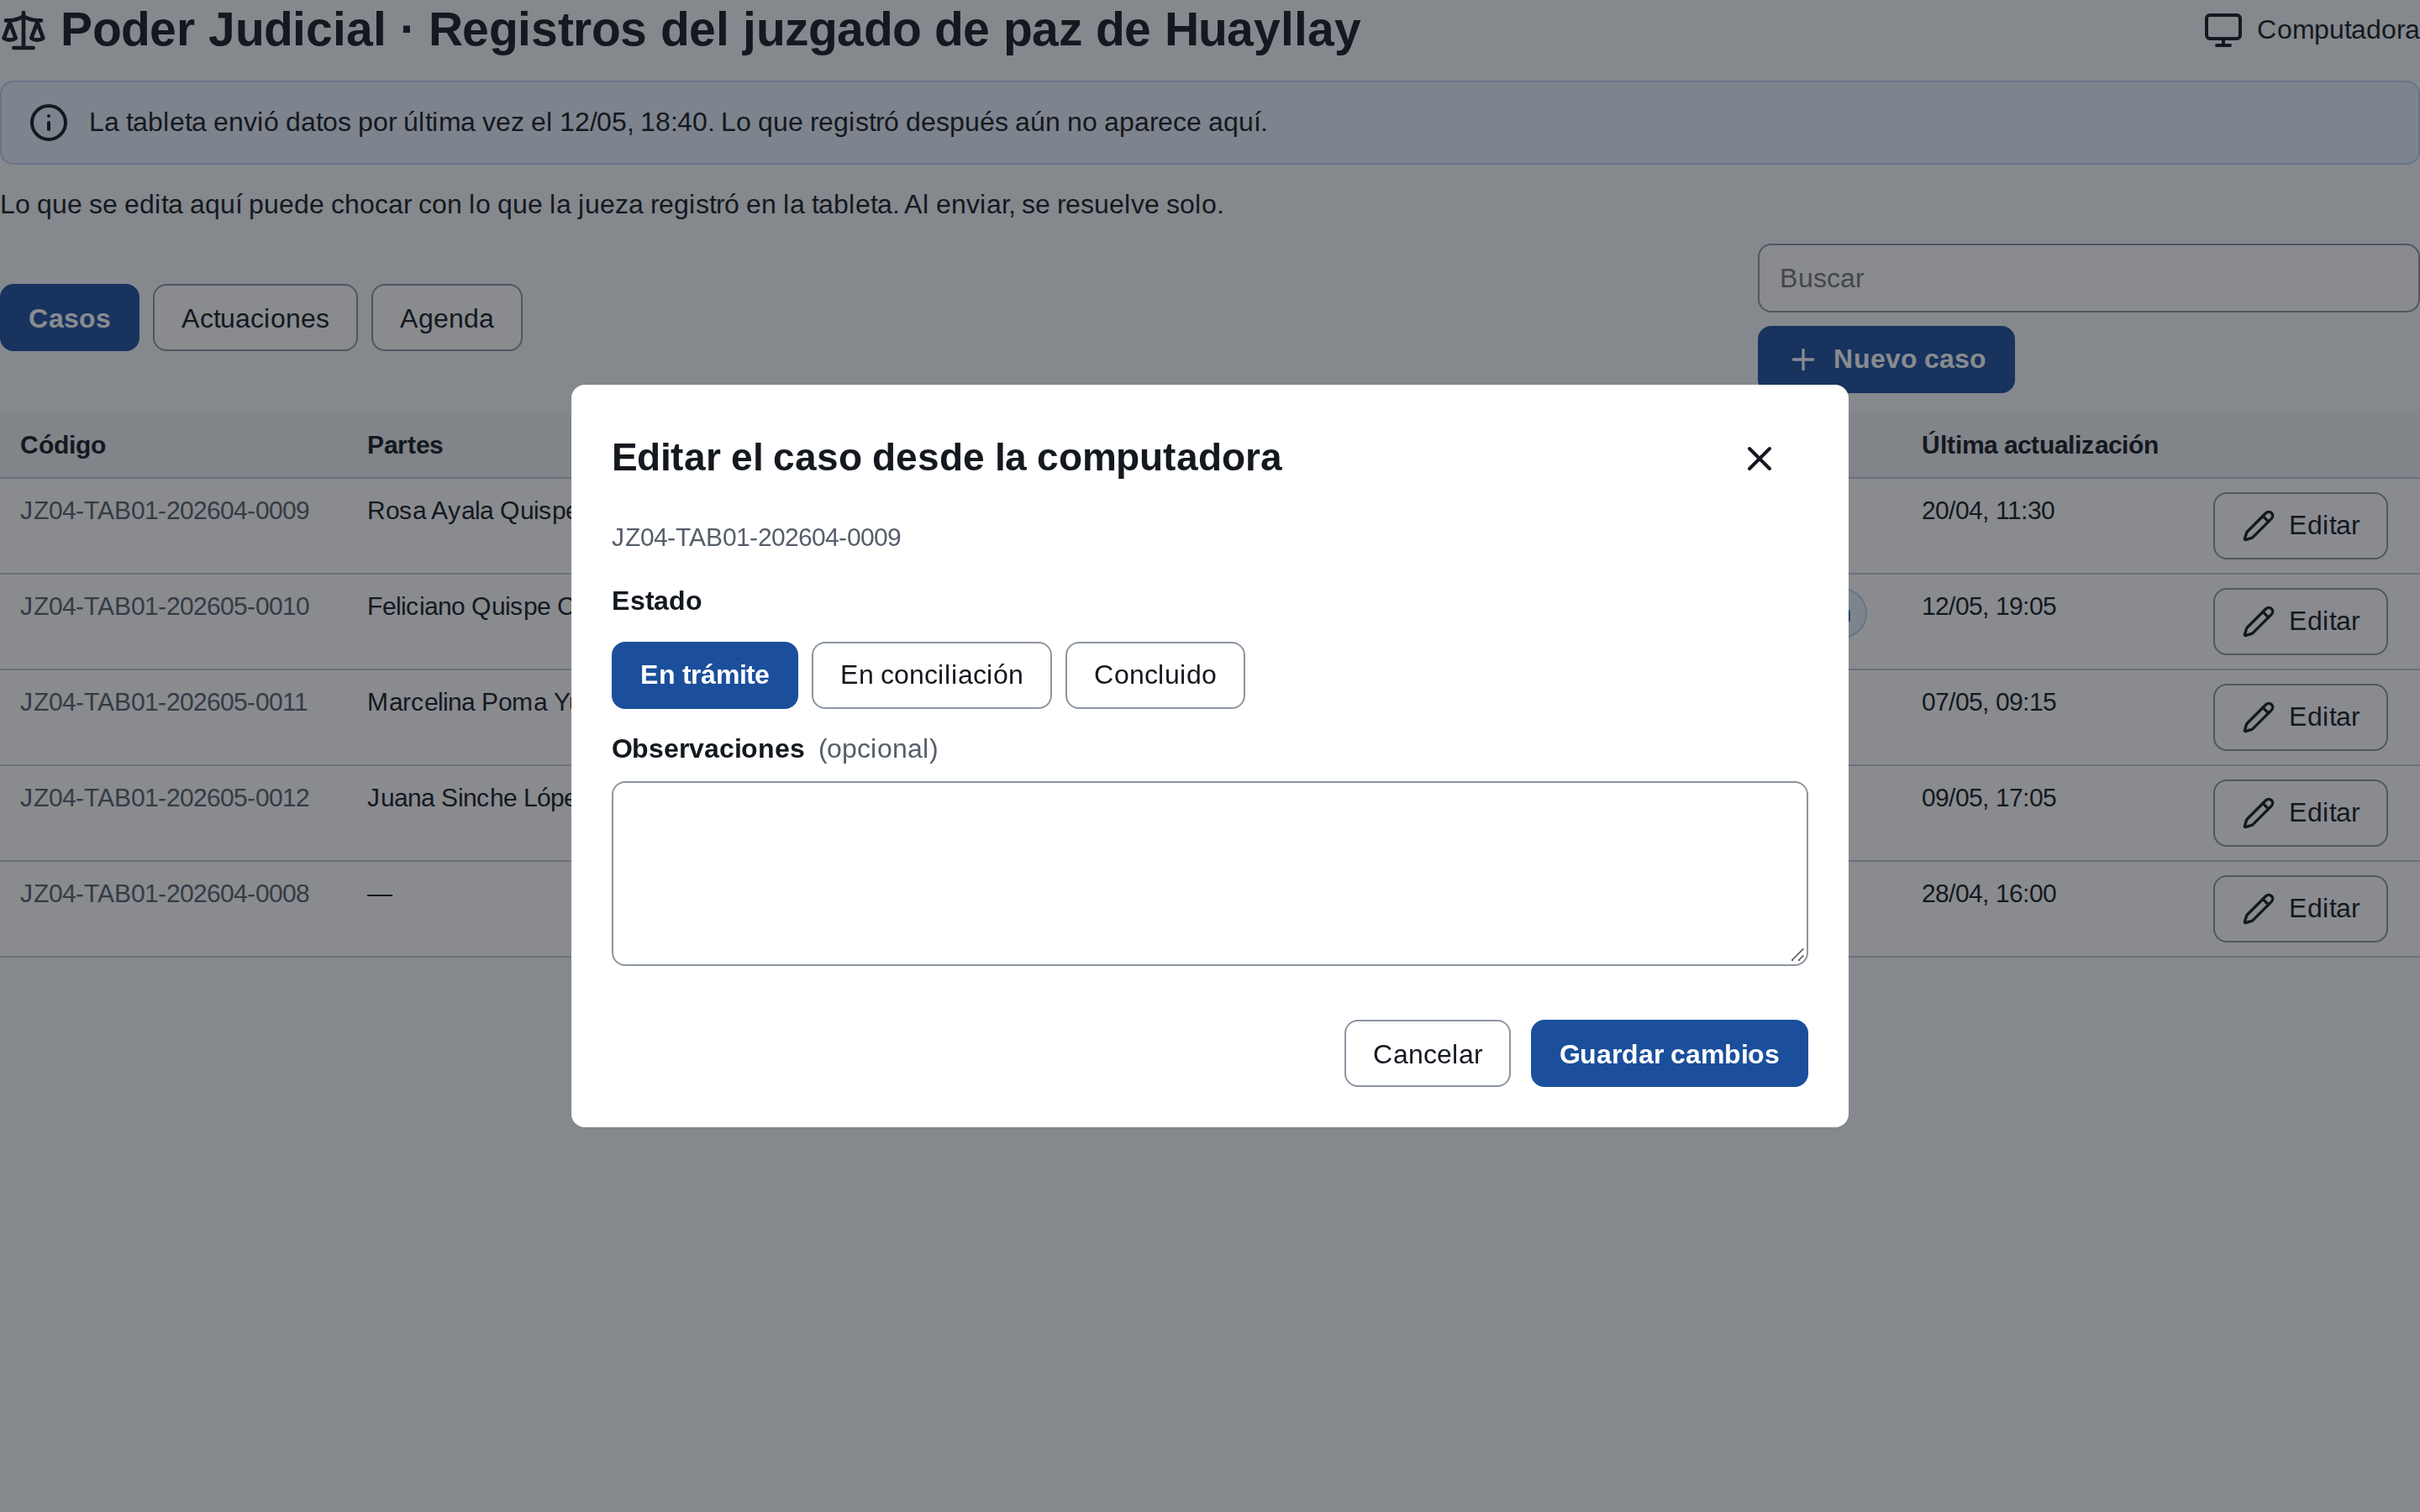
\includegraphics[width=0.82\linewidth]{capturas/FB-02_pc-editar.png}
\caption{P-10 · 2. Edición desde la computadora. Desde la computadora se puede editar, y de ahí nacen los conflictos de P-09}
\end{figure}
